\documentclass[11pt,a4paper]{article}
\usepackage[T1]{fontenc}
\usepackage[utf8]{inputenc}
\usepackage{lmodern,amsmath,amssymb,amsthm,mathtools,mathrsfs}
\usepackage[margin=27mm]{geometry}
\usepackage{microtype,booktabs,tabularx,array,enumitem,longtable}
\usepackage[dvipsnames]{xcolor}
\usepackage[colorlinks=true,linkcolor=MidnightBlue,citecolor=MidnightBlue,urlcolor=MidnightBlue]{hyperref}
\usepackage{bookmark}
\usepackage{tikz}
\usetikzlibrary{arrows.meta}
\newtheorem{theorem}{Theorem}[section]
\newtheorem{proposition}[theorem]{Proposition}
\newtheorem{lemma}[theorem]{Lemma}
\newtheorem{corollary}[theorem]{Corollary}
\theoremstyle{definition}
\newtheorem{definition}[theorem]{Definition}
\theoremstyle{remark}
\newtheorem{remark}[theorem]{Remark}
\numberwithin{equation}{section}
\newcommand{\R}{\mathbb R}
\newcommand{\dd}{\mathrm d}
\setlength{\emergencystretch}{2em}
\setlist{itemsep=3pt,topsep=5pt}
\allowdisplaybreaks[2]
\raggedbottom
\setcounter{tocdepth}{2}

\hypersetup{pdftitle={Cyclicity three for the quadratic hemicycle H14-3},pdfauthor={Haibo Lu}}
\title{Cyclicity three for the quadratic hemicycle $H_{14}^{3}$}
\author{Haibo Lu\\Shanghai Institute of Technology}
\date{Working manuscript, 19 October 2026}
\begin{document}
\maketitle
\begin{abstract}
We determine the cyclicity of the hemicycle $H_{14}^{3}$ bounding the
period annulus of the quadratic center $\dot x=-y$, $\dot y=x(1+y)$.
For all fields in a neighborhood of this center in the full
twelve-dimensional quadratic family, the isolated periodic orbits
contained in one fixed spherical neighborhood of the hemicycle have
total Poincar\'e multiplicity at most three. Arbitrarily small perturbations produce three
simple cycles, each converging to the entire hemicycle. The upper bound
compares two actual return paths in a common central-height coordinate.
Relative contraction estimates control their nonlinear terms while
retaining the divergent slow-passage actions. The signs at the entrances
then join the local critical-point bounds into a single count, including
simultaneous passage losses and unrestricted separation of two parameter
scales. A separate variation at a reversible center realizes the three
cycles in the original five-parameter subfamily. Together these arguments
give the sharp bound at this graphic with semi-hyperbolic and nilpotent
singularities at infinity.
\end{abstract}
\tableofcontents
\clearpage
\section{The hemicycle and the main result}\label{rw:main-results}

The quadratic field
\[
 \dot x=-y,\qquad \dot y=x(1+y)
\]
has a center whose period annulus fills the half-plane $y>-1$.
On the Poincar\'e sphere its outer boundary is a hemicycle: the
compactified line $y=-1$ joins two semi-hyperbolic points at infinity,
and the upper equatorial semicircle joins them through a nilpotent
point. We denote this graphic by $\Gamma=H_{14}^{3}$.
The question is how many isolated periodic orbits can appear near
this entire boundary under arbitrary quadratic perturbations.

The reduction of the quadratic finiteness problem to cyclicity
questions for a finite collection of graphics was developed by
Dumortier, Roussarie and Rousseau~\cite{DRR1994}.
For center graphics through a nilpotent point, Roussarie and Rousseau
\cite{RoussarieRousseau2015} prove finite cyclicity of the boundary
limit periodic sets for several neighboring configurations.
Their Theorem~1.1 explicitly leaves $H_{14}^{3}$ aside.
Their family $\dot x=-y+B_0x^2$, $\dot y=x+xy$ is treated for
$B_0>0$; the field above has $B_0=0$.
At the end of their introduction they identify the two
semi-hyperbolic equatorial points as the additional difficulty
in this hemicycle. A bound near a fixed positive $B_0$ does not
give a bound uniform as these points degenerate at $B_0=0$.
The hemicycles studied by Mar\'in and Villadelprat
\cite{MarinVilladelprat2025} have two hyperbolic saddles at infinity;
the semi-hyperbolic and nilpotent points here require additional
slow-passage estimates.

We use the ordinary Euclidean topology on the twelve coefficients
of a planar quadratic vector field. All neighborhoods of $\Gamma$
are taken on the closed northern hemisphere. A cycle is counted only
when its entire affine periodic orbit lies in that neighborhood.
Its multiplicity is the order of the isolated zero of a local
Poincar\'e displacement; a period annulus contributes no isolated
cycles.

\begin{theorem}[Cyclicity three]\label{rw:main:cyclicity}
Let $X_0=(-y,x(1+y))$ and let $\Gamma$ be its hemicycle described
above.
\begin{enumerate}[label=\textup{(\roman*)}]
\item There are an open neighborhood $\mathscr U$ of $\Gamma$ and
an open coefficient neighborhood $\mathscr V$ of $X_0$ such that
every quadratic field in $\mathscr V$ has total multiplicity at most
three among its isolated periodic orbits contained in $\mathscr U$.
\item For every open neighborhood $\mathscr U_1$ of $\Gamma$ and
every open coefficient neighborhood $\mathscr V_1$ of $X_0$, some
quadratic field in $\mathscr V_1$ has three distinct simple limit
cycles contained in $\mathscr U_1$.
These fields can be chosen in a sequence tending to $X_0$ such that
each of the three cycles converges to the entire $\Gamma$ in spherical
Hausdorff distance.
\end{enumerate}
Consequently the cyclicity of $H_{14}^{3}$ in the full quadratic
family is exactly three.
\end{theorem}

The upper bound controls all isolated cycles whose entire orbits lie
in the fixed neighborhood, with their full return multiplicities.
The lower bound also gives cyclicity three in the usual Hausdorff
sense of \cite[Definition~2.1]{RoussarieRousseau2015}. It is realized
in the five-parameter family
\[
 \dot x=-y+Bx^2+my^2+ax,\qquad
 \dot y=x(1+y)+cy+dy^2.
\]
Near-identity affine transformations and positive time changes make
this family a local slice for every quadratic perturbation. The two
parts of the theorem are proved independently in
Theorems~\ref{rw:upper-bound} and~\ref{rw:three-simple-cycles}.

\begin{figure}[htbp]
\centering
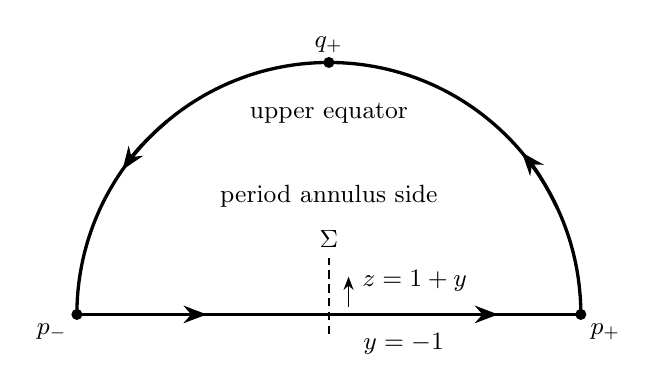
\begin{tikzpicture}[x=1cm,y=1cm,>=Stealth,font=\small]
 \draw[very thick] (-3.2,0)--(3.2,0);
 \draw[very thick] (3.2,0) arc[start angle=0,end angle=180,radius=3.2];
 \draw[->,very thick] (-2.15,0)--(-1.55,0);
 \draw[->,very thick] (1.55,0)--(2.15,0);
 \draw[->,very thick] (25:3.2) arc[start angle=25,end angle=40,radius=3.2];
 \draw[->,very thick] (130:3.2) arc[start angle=130,end angle=145,radius=3.2];
 \fill (-3.2,0) circle (2pt) node[below left] {$p_-$};
 \fill (3.2,0) circle (2pt) node[below right] {$p_+$};
 \fill (0,3.2) circle (2pt) node[above] {$q_+$};
 \node at (0,2.55) {upper equator};
 \node[below] at (0.95,-0.12) {$y=-1$};
 \draw[densely dashed,thick] (0,-0.25)--(0,0.72)
       node[above] {$\Sigma$};
 \draw[->,thin] (0.25,0.1)--(0.25,0.48);
 \node[right] at (0.3,0.42) {$z=1+y$};
 \node at (0,1.5) {period annulus side};
\end{tikzpicture}
\caption{The base hemicycle, as a topological schematic of the northern
compactification. Solid curves are the invariant finite line and the
upper equatorial arcs; arrows on these curves give the base field's
time direction. The thin arrow labels the central height, and the
dashed segment is the central transverse section. The vertices
$p_\pm$ are semi-hyperbolic and $q_+$ is nilpotent. Flattening the
compactified finite line to a diameter is schematic; distances and
curvature have no metric meaning.}
\label{rw:fig:hemicycle}
\end{figure}


\subsection{The mechanism of the proof}

Two difficulties intervene between local passage estimates and a sharp
bound. Several passages can lose their exit simultaneously, making
their linear contraction actions arbitrarily large. Near the nilpotent
end, a coefficient direction can also reveal a second scale with
unrestricted separation from the first. These phenomena require
estimates uniform in the complete passing domains. Even with such
estimates, adding the counts of neighboring charts would exceed three.
We instead compare the same two actual paths on one interval and
keep the direction in which their critical values cross zero.

The two paths start at the same outgoing point on $y=0$: one follows
the lower arc backward to the central section, and the other follows
the upper arc and the incoming lower arc forward. We compare their
outputs in the original central height $z=1+y$.
They have outputs $s_++U$ and $s_-+V$, where the reference
difference $s_--s_+$ depends on the field and is independent of the
section input. With $\epsilon>0$ the primary scale of
Definition~\ref{rw:normalization}, we study
\[
 F=U-V-(s_--s_+),\qquad
 K=\epsilon\log(V'/U').
\]
The derivatives $U',V'$ have the same nonzero sign, and
\[
 F'=U'(1-e^{K/\epsilon}).
\]
Hence $F'$ and $K$ have the same zero multiplicities. Once $K$ has
at most two zeros on that interval, Rolle's theorem gives at most
three closing zeros. If a sufficiently small cycle occurs before
the interval, it is unique and simple. It supplies a signed entrance
at which the bound for $K$ improves to one, leaving at most two
further closing zeros. Section~\ref{rw:counting} states the precise
thresholds and proves this counting implication.

Two additional facts make this implication applicable to the whole
hemicycle. The bounded-energy orbits and the large-energy orbits on
which the coefficients remain small are counted together by one
source return. Whenever one monotone comparison does not already
settle the outer cycles, an outer cycle supplies a coefficient
inequality and bounds three equilibrium-free returning strips.
Every intermediate input, including a nonclosing one, then
has both complete central outputs. This is the physical interval
proved in Proposition~\ref{rw:saturation}. The source bound is not
added to a count on this interval when it already includes those
source cycles.

Proposition~\ref{rw:ordered-cover} arranges the physical interval as
a regular prefix followed by at most one terminal union. The regular
crossings have one direction and supply the signs at its entrance.
The hardest endpoint charts initially allow four closing zeros.
Their derivative estimates alone therefore do not prove the theorem.
On a fixed coefficient fibre, Proposition~\ref{rw:coefficient-transport}
transports the outer-cycle inequality to each actual open overlap.
The three-saddle and weak-end arguments then use the already fixed
entrance to obtain a two-zero bound for $K$ on the whole union,
with a one-zero bound under the small-cycle entrance.
These are the exceptional steps in Propositions
\ref{rw:anchors:three-saddle} and \ref{rw:anchors:primary-weak};
Proposition~\ref{rw:anchored-unions} joins them to the other endpoints.

At secondary scale the entrance is carried through the
primary--wedge--secondary regular chain; the actual saddle ratio
and the increasing weak numerator give the terminal bounds in
Propositions~\ref{rw:secondary:saddle-anchor}
and~\ref{rw:secondary:weak-anchor}.

Sections~4--5 construct the original passages and their real center
comparison domains before coefficient division. Relative amplitudes
are estimated separately from possibly divergent contraction actions.
This distinction permits simultaneous small gaps, moving weak roots
and exact cancellation of common powers. Sections~7--10 then classify
the finite, infinite and secondary endpoints on their whole passing
domains. The long secondary passage retains its exact scale exponent
even when the product of the primary scale and the logarithm of the
secondary scale is unbounded.

The lower bound starts from the reversible face $B=0$, $m=\epsilon$.
Section~\ref{rw:lower:preview} describes its three-root variation after
the basic passages and real centers are available.
Section~\ref{rw:lower-bound-section} constructs the coefficient curve,
preserves all three real return paths for one field, and proves that
each resulting cycle approaches the entire hemicycle.

The appendices provide the independent Abelian-integral threshold,
the common-domain calculus, the endpoint algebra and uniform relative
estimates. The domains and derivative orders are stated with the
transitions and endpoint comparisons that use them.

\section{Geometry and the return problem}\label{rw:geometry}

We count cycles on one transverse section in a fixed neighborhood of
the hemicycle.  The geometric construction ensures that every counted
cycle crosses this section exactly once.  We then define the return
on the inputs whose finite return paths stay in the neighborhood;
the later changes of scale estimate this same return problem.

The base field is
\begin{equation}\label{rw:base-field}
 X_0:\qquad \dot x=-y,\qquad \dot y=x(1+y).
\end{equation}
Put $z=1+y$.  On $z>0$ it has the first integral
\begin{equation}\label{rw:geometry:energy}
 H_0(x,z)=\frac{x^2}{2}+z-1-\log z.
\end{equation}
Its Hessian is $\operatorname{diag}(1,z^{-2})$, its unique critical
point is $(0,1)$, and its sublevel sets are compact in $z>0$.
Consequently every positive level is a smooth strictly convex oval.
The field is nonzero on that oval and tangent to it, so the oval is a
periodic orbit.

We use the northern embedding
\[
 \iota(x,y)=\frac{(x,y,1)}{\sqrt{1+x^2+y^2}}.
\]
The boundary of this period annulus on the sphere is the Jordan curve
$\Gamma$ consisting of the closure of $y=-1$ and the upper equatorial
semicircle.  Indeed, at bounded $x$ the lower branch of a level tending
to infinity approaches $y=-1$.  Every unbounded sequence on these
ovals has $y>-1$ and hence can accumulate only on the upper semicircle;
intersections with each fixed ray $y=k|x|$, $k\ge0$, tend to infinity,
as does the upper turning point.  Write $p_-,p_+$ for the negative and
positive horizontal points at infinity, and $q_+$ for the positive
vertical point.  The direction on $y=-1$ is from $p_-$ to $p_+$.
In the chart $y=1/r$, $x=w/r$, multiplication by $r>0$ gives
\[
 r'=-rw(1+r),\qquad w'=-w^2-r(1+w^2).
\]
Thus the other half of $\Gamma$ runs from $p_+$ through $q_+$ to $p_-$.

\subsection{A coefficient family for all quadratic perturbations}

Consider the five-parameter family
\begin{equation}\label{rw:family}
 \begin{aligned}
 X_\alpha=(P_\alpha,Q_\alpha),\qquad
 P_\alpha&=-y+Bx^2+my^2+ax,\\
 Q_\alpha&=x(1+y)+cy+dy^2,
 \qquad \alpha=(B,m,a,c,d).
 \end{aligned}
\end{equation}
The coefficient which breaks the invariant line is
\begin{equation}\label{rw:geometry:line-breaking}
 \ell=d-c,\qquad \dot z\big|_{z=0}=\ell.
\end{equation}
The origin remains an equilibrium; its linearization has determinant
$1+ac>0$ near $\alpha=0$.

\begin{proposition}\label{rw:slice}
The family \eqref{rw:family}, near-identity affine coordinate changes,
and positive constant time changes form analytic local coordinates on
the twelve-dimensional space of real quadratic planar vector fields
near $X_0$.  A uniform bound for isolated cycles of \eqref{rw:family}
in a fixed spherical collar of $\Gamma$, counted with return-germ
multiplicity, therefore gives the same bound on a smaller fixed collar
for every quadratic field in an open coefficient neighborhood of $X_0$.
\end{proposition}

\begin{proof}
For $A$ near the identity matrix, $b\in\R^2$ near zero, and $r\in\R$
near zero, define
\[
 \mathcal S(A,b,r,\alpha)(v)
       =e^r A^{-1}X_\alpha(Av+b).
\]
There are four matrix entries, two translation parameters, one time
parameter, and five parameters in $\alpha$.
For an affine infinitesimal change $h$, its column in the differential
at the base point is $DX_0h-DhX_0$.  The changes
$(1,0),(0,1),(x,0),(y,0),(0,x),(0,y)$ give, respectively,
\[
 \begin{array}{lll}
 v_1=(0,1+y),&v_2=(-1,x),&v_3=(y,x+xy),\\
 v_4=(-x-xy,y+y^2),&v_5=(-x,x^2+y),&v_6=(-y,-x).
 \end{array}
\]
The time column is $v_7=(-y,x+xy)$.  The remaining columns, in the
parameter order of \eqref{rw:family}, are
\[
 (x^2,0),\quad(y^2,0),\quad(x,0),\quad(0,y),\quad(0,y^2).
\]
In a linear relation, the constant, first-component $xy$ and
second-component $x^2$ coefficients eliminate $v_1,v_2,v_4,v_5$.
The remaining coefficients $u,v,w$ of $v_3,v_6,v_7$ satisfy
\[
 \begin{pmatrix}1&-1&-1\\1&-1&1\\1&0&1\end{pmatrix}
 \begin{pmatrix}u\\v\\w\end{pmatrix}=0.
\]
Its determinant is $-2$, and the five family columns occupy distinct
monomials. Thus $D\mathcal S$ is invertible; the analytic inverse
function theorem proves the local-coordinate assertion.

If $Y=\mathcal S(A,b,r,\alpha)$ and $\Phi(v)=Av+b$, then
$D\Phi\,Y=e^r X_\alpha\circ\Phi$.  Thus $\Phi$ sends trajectories to
trajectories preserving time orientation.  On transverse sections it
conjugates the corresponding return germs.  If $\psi$ is the section
coordinate change and $P$ a return, then
\begin{equation}\label{rw:geometry:section-unit}
 \psi(P(u))-\psi(u)
 =(P(u)-u)\int_0^1\psi'\bigl(u+t(P(u)-u)\bigr)\,\dd t.
\end{equation}
At a fixed point the last factor is nonzero.  Isolation and the order
of the displacement zero are preserved.

In homogeneous coordinates the spherical extension of $\Phi$ is
\[
 \widehat\Phi(\xi_1,\xi_2,\xi_3)
 =\frac{(A(\xi_1,\xi_2)^{\mathsf T}+b\xi_3,\xi_3)}
 {\left\|(A(\xi_1,\xi_2)^{\mathsf T}+b\xi_3,\xi_3)\right\|}.
\]
Its homogeneous matrix is invertible, so it is a sphere
diffeomorphism preserving the closed northern hemisphere.  It converges
uniformly to the identity as $(A,b)$ tends to $(I,0)$.  Given a collar
$U_*$ for the normalized family, choose $U$ with
$\overline U\subset U_*$.  One sufficiently small affine neighborhood
then satisfies $\widehat\Phi(\overline U)\subset U_*$ for every such
$\Phi$.  Intersecting the corresponding product neighborhood with the
local-coordinate neighborhood of $\mathcal S$ gives an open
twelve-dimensional coefficient neighborhood.  Cycles in $U$ map
injectively to cycles in $U_*$ with their multiplicities unchanged.
\end{proof}

\subsection{A fixed collar and its transverse section}

The initial energy count uses the base-field Chebyshev estimate of
Proposition~\ref{rw:base-ect}.  Fix its threshold
$H_{\mathrm{ECT}}$ and choose the collar so that every point on its
positive lower section has energy above that threshold.

\begin{proposition}\label{rw:collar}
There are a closed spherical annulus $\mathcal A$ containing $\Gamma$
in its interior, a number $0<z_L<1/8$, and a coefficient neighborhood
$\mathcal V$ of zero with the following properties.  The annulus
excludes the origin and the negative vertical point at infinity, and
\begin{equation}\label{rw:geometry:section}
 h(z_L):=z_L-1-\log z_L>H_{\mathrm{ECT}}+2,
 \qquad \Sigma=\{x=0,\ |z|<z_L\}.
\end{equation}
Its lower part over $-1\le x\le1$ is the rectangle
$[-1,1]\times[-z_L,z_L]$ in $(x,z)$ coordinates.
Every affine periodic orbit contained in $U=\operatorname{int}\mathcal A$
is essential in $\mathcal A$ and crosses $\Sigma$ exactly once, with
$\dot x>0$.  Both $\mathcal A$ and $\mathcal V$ can be chosen invariant
under the spatial and coefficient reflections defined below.
\end{proposition}

\begin{proof}
We first choose three vertex boxes in which no periodic orbit can be
contained.  Throughout this construction let all five coefficient
moduli be at most $p_*=1/64$.
At a horizontal vertex put $x=\sigma/r$, $y=v/r$, where
$\sigma\in\{-1,1\}$, and multiply the field by $r>0$.  Its equations
are
\[
 \begin{aligned}
 r'&=-\sigma Br-\sigma mrv^2+\sigma r^2v-ar^2,\\
 v'&=\sigma r+\sigma(1-B)v+dv^2-\sigma mv^3
          +\sigma rv^2+(c-a)rv.
 \end{aligned}
\]
The divergence of this polynomial field is
\[
 \sigma(1-2B)+2dv-4\sigma mv^2+4\sigma rv+(c-3a)r.
\]
On the square $|r|,|v|\le1/8$ its difference from $\sigma$ is at
most $109/1024<1/8$.  If a periodic orbit were contained in its
northern part $r>0$, its Jordan disk would lie in the same square
and half-plane.  Green's theorem would give zero for the integral
of the divergence over that disk, contrary to its strict sign.

At the upper vertex use $y=1/r$, $x=w/r$.  The positively rescaled
field is $r'=-rF$, $w'=G$, where
\[
 \begin{aligned}
 F&=(1+r)w+d+rc,\\
 G&=m-dw+(B-1)w^2+r[-1+(a-c)w-w^2].
 \end{aligned}
\]
In $0<r<1/4$, $|w|<1/4$, an equilibrium lies on
\[
 w=w_s(r)=-\frac{d+rc}{1+r},\qquad
 |w_s|\le p_*,\quad |w_s'|\le2p_*.
\]
On this graph,
\[
 G_r\le-1+2p_*^2,\qquad |G_w|\le4p_*+2p_*^2,
\]
so
\[
 \frac{\dd}{\dd r}G(r,w_s(r))
 \le-1+10p_*^2+4p_*^3<-\frac12.
\]
There is at most one equilibrium in the box, and its determinant is
\[
 \det D(-rF,G)
 =r(1+r)\frac{\dd}{\dd r}G(r,w_s(r))<0.
\]
It is a saddle.  A periodic orbit contained in this rectangle would
enclose either no equilibrium or one saddle, whereas its index is one.
This excludes such an orbit.

Cut the regular parts of $\Gamma$ at finitely many points, with two
cuts inside each vertex box.  The remaining compact regular arcs have
flow-box neighborhoods.  A sufficiently thin bicollar can be divided
by radial crosscuts into strips, each contained in one of these flow
boxes or vertex boxes.  Make the crosscuts transverse at the chosen
regular points, with their positive normal pointing in the direction
of the base flow.  Include the lines $x=-1,0,1$ on the finite arc
and choose the stated rectangular part there.  Its width can be made
arbitrarily small; choose $z_L$ to satisfy
\eqref{rw:geometry:section}.  The other widths can then be decreased
so that the annulus excludes the two points specified in the statement.
The construction can be made symmetric under $x\mapsto-x$ by choosing
the two horizontal boxes and the regular crosscuts in reflected pairs.

On the central rectangle, $P_\alpha>3/4$ after shrinking the
coefficient neighborhood.  On every other crosscut the normal
component also has a positive minimum on its compact length.  The
finitely many strict inequalities persist on one common coefficient
neighborhood, which we intersect with its reflected image.

Any periodic orbit in $U$ must meet a crosscut.  Otherwise it is
contained in a single strip, where a flow-box coordinate or one of the
vertex arguments excludes it.  All crosscut intersections are transverse
and positive.  There are finitely many, since the orbit is compact and
a transverse intersection is isolated.  Each crosscut represents the
same relative homology class in the annulus, so its signed intersection
number with the orbit is the orbit's winding number.  A simple closed
curve in an annulus has winding number $0$ or $\pm1$; positivity
forces the value one.  Hence the orbit is essential and meets every
crosscut, in particular $\Sigma$, exactly once.
\end{proof}

\subsection{Actual returns and periodic points}

Only isolated affine periodic orbits whose northern images lie in $U$
are counted.  We first locate these orbits relative to the line $z=0$
and bound the line-breaking coefficient by their section height.  The
return domain will then be defined by the complete trajectory.

\begin{lemma}\label{rw:geometry:cycle-height}
Every periodic orbit contained in $U$ encloses the origin and lies in
$z>0$.  If $s$ is its intersection with $\Sigma$, then
\begin{equation}\label{rw:geometry:line-bound}
 0<s<z_L,\qquad |\ell|<3s.
\end{equation}
\end{lemma}

\begin{proof}
An essential curve in $\mathcal A$ separates its two complementary
components.  The origin is on the bounded side of $\Gamma$, while
the southern hemisphere is on the other side.  Thus the affine Jordan
disk of each such periodic orbit contains the origin.

For $\ell\ne0$, every intersection with $z=0$ has the same nonzero
normal velocity $\ell$.  A periodic scalar function cannot have only
crossings of one sign, so a periodic orbit cannot meet this line.
For $\ell=0$, invariance and uniqueness give the same exclusion.
Choose one of the regular equatorial crosscuts of the preceding
construction with its northern part in $y>0$.  Every counted orbit
meets it, and hence is on the side $z>0$ throughout.

Its lower segment is a graph over $[-1,1]$, since $P_\alpha>3/4$
on the central rectangle.  On that graph the exact equation is
\[
 z_x=\ell A(x,z)+b(x,z)z,
 \quad A=\frac{(1-z)^2}{D},\quad
 b=\frac{x+c(z-1)}{D},
\]
where
\[
 D=1-z+Bx^2+m(1-z)^2+ax.
\]
For $0\le z\le z_L<1/8$ and the coefficient bound used above,
$3/4<D<9/8$, $A>2/3$, and $|b|<3/2$.
If $\ell<0$, integrate from $0$ to $1$ and use $z(1)>0$ to obtain
\[
 s>|\ell|\int_0^1 A(t,z(t))
             e^{-\int_0^t b(u,z(u))\,\dd u}\,\dd t
 \ge\frac49(1-e^{-3/2})|\ell|>\frac{|\ell|}{3}.
\]
If $\ell>0$, variation of constants from $-1$ to $0$ gives the same
lower bound for $s$ after discarding its positive homogeneous term.
The case $\ell=0$ is immediate.
\end{proof}

Let $\Sigma_+=\{x=0,\ 0<z<z_L\}$, identified with $(0,z_L)$.
For a fixed $\alpha$, define $\mathcal D_\alpha$ to be the set of
$s\in\Sigma_+$ whose trajectory has a finite first positive-time
return to $\Sigma_+$, with the entire intervening path affine,
contained in $U$, and contained in $z>0$.  Write this return as
$\mathcal P_\alpha(s)$.

\begin{lemma}\label{rw:geometry:return-domains}
The domain $\mathcal D_\alpha$ is open.  The return is locally jointly
analytic in its input and coefficients and is a local increasing
diffeomorphism.  Its isolated fixed points correspond bijectively to
the cycles counted in $U$.
\end{lemma}

\begin{proof}
A finite return path is compact in the prescribed open region and
ends transversely. Analytic flow dependence and the implicit function
theorem preserve its return under small input and coefficient changes.
Compactness away from the endpoint flow boxes, and transversality
inside them, exclude an earlier intersection. This proves openness
and local joint analyticity.
The variational determinant formula for a transverse return gives
\[
 \mathcal P_\alpha'(s)=
 \frac{P_\alpha(0,s-1)}
      {P_\alpha(0,\mathcal P_\alpha(s)-1)}
 \exp\!\left(\int_0^{T(s)}\operatorname{div}X_\alpha
                          (\Phi_t^\alpha(0,s-1))\,\dd t\right)>0.
\]
Here $P_\alpha$ is the first component of the vector field in
\eqref{rw:family}.
Both normal velocities are positive.  Finally, a fixed point closes
the prescribed trajectory, and a counted cycle has exactly one section
intersection by Proposition~\ref{rw:collar} and belongs to this domain
by Lemma~\ref{rw:geometry:cycle-height}.
\end{proof}

\begin{definition}\label{rw:geometry:counting}
The Poincar\'e multiplicity of an isolated cycle is the order of the
zero of $\mathcal P_\alpha(s)-s$ at its section intersection.  A return germ
identically equal to the identity contributes no isolated cycle.
\end{definition}

This definition is independent of the analytic section coordinate by
\eqref{rw:geometry:section-unit}.  Multiplication of a displacement by
an analytic nonvanishing factor also preserves its zero orders.
Derivative zeros require a separate comparison, since differentiating
a unit multiple also differentiates the unit.  The domain
$\mathcal D_\alpha$ may be disconnected.  Thus a periodic orbit
supplies a local return, while a comparison with more distant section
points requires the intervening paths to be constructed.

\subsection{One direction for each fixed field}

The reflection used throughout the paper reverses time as well as space.
Let
\begin{equation}\label{rw:geometry:reflection}
 R(x,y)=(-x,y),\qquad
 \alpha^R=(B,m,-a,-c,-d).
\end{equation}
Direct substitution in \eqref{rw:family} gives
\begin{equation}\label{rw:geometry:flow-reflection}
 X_{\alpha^R}(R v)=-DR\,X_\alpha(v),\qquad
 \Phi_t^{\alpha^R}(Rv)=R\Phi_{-t}^{\alpha}(v).
\end{equation}
The collar and coefficient neighborhood are reflection invariant, and
$R$ fixes every point of $\Sigma_+$.  Thus it preserves cycles, their
central height, and isolation.

Let $s_*$ be a periodic point and restrict its original
forward return to an analytic increasing diffeomorphism
$P:I\to P(I)$ on a small positive section interval.  The reflected
forward return near that point is $Q=P^{-1}:P(I)\to I$, and
\begin{equation}\label{rw:geometry:inverse-germ}
 Q(s)-s=-\bigl(P(Q(s))-Q(s)\bigr).
\end{equation}
Since $Q'(s_*)>0$, composition with $Q$ preserves the order of the
displacement zero.  The multiplicity is therefore unchanged by
\eqref{rw:geometry:reflection}.  This is an identity of germs at a
periodic point.  The reflected positive return follows the original
trajectory in reverse time, so its domain is determined by that reverse
passage.

We may consequently reflect a fixed field with $\ell<0$ and carry out
its count with $\ell\ge0$.  All section labels and comparison paths
for that field are thereafter taken in this selected direction.
Numerical cutoffs used uniformly in the family are chosen once on a
reflection-invariant coefficient neighborhood, not chosen anew for
each field.  This sign-dependent choice is made only after the field
is fixed.  Coefficient differentiation and division across $\ell=0$
use the original analytic auxiliary maps on their stated common domains.

\subsection{Energy ranges and the primary normalization}

The lower section has the analytic coordinate
\[
 h=h(s)=s-1-\log s>H_{\mathrm{ECT}}+2,
 \qquad h'(s)=1-s^{-1}<0.
\]
For $0<\eta<1$ and a fixed $H_*>h(z_L)+1$, set
\[
 \mathscr M(h)=\max\{|B|h,|m|h,|a|\sqrt h,|c|\sqrt h\}.
\]
The three energy classes are
\begin{equation}\label{rw:geometry:energy-classes}
 \begin{array}{ll}
 h\le H_*,&\text{bounded energy},\\
 h>H_*,\quad\mathscr M(h)\le\eta,
       &\text{small coefficients at the energy scale},\\
 h>H_*,\quad\mathscr M(h)>\eta,
       &\text{parameter-dominant energy}.
 \end{array}
\end{equation}
The first two classes will be counted together.  Their thresholds are
fixed before the final coefficient shrink, and the bounded-energy
interval lies entirely above $H_{\mathrm{ECT}}$.
This classification applies to actual periodic
points and extends no return domain.

\begin{definition}\label{rw:normalization}
The primary scale and normalized coefficients, for $\rho>0$, are
\begin{equation}\label{rw:geometry:primary-scale}
 \begin{gathered}
 \rho=\max\{\sqrt{|B|},\sqrt{|m|},|a|,|c|\},
 \qquad\epsilon=\rho^2,\\
 (B,m,a,c)=(\rho^2\bar B,\rho^2\bar m,
                       \rho\bar a,\rho\bar c),\qquad
 \nu=\ell/\rho,\quad\bar d=d/\rho=\bar c+\nu.
 \end{gathered}
\end{equation}
Thus $\max(|\bar B|,|\bar m|,|\bar a|,|\bar c|)=1$.
The generators in original and primary coefficients are
\begin{equation}\label{rw:geometry:generators}
 \begin{gathered}
 \tau_0=a+c,\qquad\sigma_0=c(B+m),\\
 \tau_1=\bar a+\bar c=\tau_0/\rho,\qquad
 \sigma_1=\bar c(\bar B+\bar m)=\sigma_0/\rho^3.
 \end{gathered}
\end{equation}
\end{definition}

The normalized vector lies on the union of the signed faces of
$[-1,1]^4$.  Smooth parameter arguments are made in the indicated
local coefficient charts, not by differentiating the maximum across
its corners.  For $\rho>0$, the two products $\tau_0\sigma_0$ and
$\tau_1\sigma_1$ have the same sign, but
\begin{equation}\label{rw:geometry:generator-ratio}
 \frac{\tau_1}{\sigma_1}
       =\epsilon\frac{\tau_0}{\sigma_0}\qquad(\sigma_0\ne0).
\end{equation}
If $\rho=0$, then $B=m=a=c=0$, while $d=\ell$ may be nonzero.
All energies belong to the first two classes because $\mathscr M=0$.
No barred coefficients, $\nu$, or quotient by $\epsilon$ is used in
that case.

For later calculations we record the exact scaled equations.  With
$\xi=t/\rho$, $X=\rho x$, and $z=1+y$, the lower equations are
\begin{equation}\label{rw:geometry:lower-field}
 \begin{aligned}
 X_\xi&=\epsilon\{1-z+\bar B X^2+\bar aX
                              +\epsilon\bar m(1-z)^2\},\\
 z_\xi&=Xz+\epsilon\bar c\,z(z-1)+\rho\ell(1-z)^2.
 \end{aligned}
\end{equation}
With $X=\rho x$ and $Y=\rho^2y$, the same field and time give
\begin{equation}\label{rw:geometry:upper-field}
 \begin{aligned}
 X_\xi&=Y(\bar mY-1)+\epsilon(\bar B X^2+\bar aX),\\
 Y_\xi&=(Y+\epsilon)(X+\bar cY)+\nu Y^2.
 \end{aligned}
\end{equation}
These identities do not assume that $\nu$ is bounded.

\begin{lemma}\label{rw:geometry:flatness}
A parameter-dominant cycle has $\rho>0$ and satisfies
\[
 \rho\sqrt h>\eta,\qquad
 |\ell|<3e^{-\eta^2/\rho^2},\qquad
 \frac{|\ell|}{\rho^k}\le C_{k,\eta}
                  e^{-\eta^2/(2\rho^2)}\quad(k\ge0).
\]
\end{lemma}
\begin{proof}
If $\rho\sqrt h\le\eta$, the four terms in $\mathscr M(h)$ are
bounded by $\eta^2,\eta^2,\eta,\eta$, respectively, contradicting
the third class.  Since $0<s<1$, the exact identity
$s=e^{-h-1+s}$ gives $s<e^{-h}$.  Apply
\eqref{rw:geometry:line-bound} and retain half of the exponential to
absorb any fixed power of $\rho^{-1}$.
\end{proof}
The estimate uses the height of an actual cycle.  The ratio $\ell/s$
still has only the bound in \eqref{rw:geometry:line-bound}; derivatives
along parameter curves require the common-domain estimates below.

\begin{lemma}\label{rw:geometry:endpoints}
Every periodic orbit counted in $U$ meets $y=0$ exactly once on each
half-axis.  For $\rho>0$, write these intersections, in the selected
direction, as $(p/\rho,0)$ and $(-q/\rho,0)$ with $p,q>0$.
The upper connecting arc lies in $y>0$.  Nested cycles have increasing
$p$ and $q$ towards the outer cycle.  Reflection exchanges the labels:
$p_{\rm ref}=q_{\rm orig}$ and $q_{\rm ref}=p_{\rm orig}$.
\end{lemma}
\begin{proof}
By Lemma~\ref{rw:geometry:cycle-height}, the Jordan disk contains
the origin.  Each horizontal half-axis therefore meets its boundary.
On $y=0$, the normal velocity is $\dot y=x$, so all crossings of
the positive ray are upward and all crossings of the negative ray
are downward.  Their signed intersection number is the winding number
one; consequently each ray is crossed exactly once.  The arc between
the upward and downward crossings is in $y>0$.  Inclusion of the
Jordan disks orders their two ray intersections and proves the nesting
assertion.  Equation~\eqref{rw:geometry:flow-reflection} exchanges the
two crossings while reversing time, giving the last assertion.
\end{proof}

In particular a cutoff imposed on the reflected outgoing label is a
cutoff on the original incoming label, not on the original outgoing
label.  All later endpoint cutoffs refer to the direction already
selected for the fixed field.  Varying a section input always keeps
the original coefficient vector fixed; any induced changes of scaled
coordinates must be included in the chain rule.

\section{A conditional reduction to three closing zeros}
\label{rw:counting}

The sharp count uses one passing interval for the selected outer
cycles.  Four statements about a fixed field provide this interval
and its zero bounds: the initial energy classes have a joint count,
an outer cycle supplies the complete comparison paths, the logarithmic
derivative ratio has at most two zeros there, and a small cycle forces
a stronger entrance sign.  We prove the resulting count here.
Sections~6, 11 and 12 establish these hypotheses on the same interval.

\subsection{Multiplicity and the three counting levels}

On a regular section interval, all derivatives in this section are taken
with the original field fixed.  If $f$ is real analytic on a neighborhood
of an interval $J$, write $Z(f;J)$ for the sum of the orders of its isolated
zeros in $J$.  The identically zero function contributes no isolated zeros.  At an
included finite endpoint we count the full order of the analytic germ,
not a one-sided order.  For an open or unbounded interval a bound for $Z$
means the same bound for every finite selection of zeros with their full
multiplicities.  No regular extension at an excluded singular endpoint is
implicit in this convention.

\begin{lemma}[Rolle's inequalities with multiplicity]
\label{rw:counting:rolle}
For a real analytic function on a neighborhood of an interval $J$,
\begin{equation}\label{rw:counting:ordinary-rolle}
 Z(f;J)\le Z(f';J)+1
\end{equation}
whenever the right-hand side is finite.  Suppose in addition that $a$ is
the left endpoint of $J$, $f$ extends analytically across $a$, and
$f(a)f'(a)>0$.  On the part of $J$ to the right of $a$,
\begin{equation}\label{rw:counting:away-rolle}
 Z(f;J)\le Z(f';J).
\end{equation}
For a right entrance the corresponding condition is $f(a)f'(a)<0$.
Equivalently, in either case the derivative in the direction from the
entrance into the interval must have the same sign as $f(a)$.
\end{lemma}
\begin{proof}
For any finite selection of zeros, differentiation lowers each order
by one and Rolle gives an additional zero between consecutive zeros;
this proves \eqref{rw:counting:ordinary-rolle}. Under the left-entrance
condition, after changing signs, \(f(a),f'(a)>0\). Before the first
selected zero, the derivative must change from positive to negative,
supplying one additional derivative zero. This proves
\eqref{rw:counting:away-rolle}; reverse the coordinate at a right
entrance. Constant functions have no isolated zeros.
\end{proof}

Now assume $\rho>0$ and put $\epsilon=\rho^2$.  Let two comparison
paths be defined on one open passing interval $I$, with analytic central outputs
$s_++U(t)$ and $s_-+V(t)$.  The central coordinate is the original
height $z=1+y$.  The reference values $s_\pm$ are fixed while $t$ varies;
in the applications their difference is
\[
 s_--s_+=\rho\nu H=\ell H,\qquad H>0,
\]
where $H$ may depend on the field but not on the input.  Assume that
$U'$ and $V'$ are nonzero and have the same sign throughout $I$.
Define
\begin{equation}\label{rw:counting:levels}
 F=U-V-\rho\nu H,\qquad
 K=\epsilon\log\frac{V'}{U'},\qquad
 M=wK',\qquad w>0.
\end{equation}
The multiplier $w$ is real analytic and positive on $I$.
It may tend to zero or infinity at an excluded singular
endpoint.  Only the positivity of $V'/U'$ is needed to define $K$;
neither derivative is required to be positive individually.

\begin{lemma}[Closing differences and logarithmic ratios]
\label{rw:zero-calculus}
Under these hypotheses, on every interval $J\subset I$,
\begin{equation}\label{rw:counting:levels-count}
 \begin{split}
 Z(F';J)&=Z(K;J),\\
 Z(K';J)&=Z(M;J),\\
 Z(F;J)&\le 1+Z(K;J)\le 2+Z(M;J),
 \end{split}
\end{equation}
provided the indicated bounds are finite.  The statements include
multiplicities.  If an outward entrance for $K$ is available, the second
Rolle step improves to $Z(K;J)\le Z(M;J)$ on the interval beyond that
entrance.
\end{lemma}
\begin{proof}
The input-independent reference difference disappears upon
differentiation, giving the exact identity
\[
 F'=U'\bigl(1-e^{K/\epsilon}\bigr).
\]
The function $(1-e^{v/\epsilon})/v$ extends analytically and is
nonzero at $v=0$, with value $-1/\epsilon$.  Consequently $F'$ and
$K$ have precisely the same zero orders.  Multiplication by $w$ likewise
preserves the zero orders of $K'$.  Apply
Lemma~\ref{rw:counting:rolle} first to $F$, then to $K$.
If $K$ is constant, $F$ is constant or strictly monotone; this also
settles the constant cases.  The entrance improvement is
\eqref{rw:counting:away-rolle} applied to $K$.
\end{proof}

The passage from $M$ to closing zeros therefore uses two Rolle steps,
through $K$ and then $F$.  A signed entrance for $K$ improves the first
step; the step from $K$ to $F$ still costs one zero.  The functions
$U,V$ include every regular connection along their respective paths,
so those connections also enter the derivative ratio.

The following elementary observation will join local estimates without
adding their bounds.

\begin{lemma}[Joining crossings of one sign]
\label{rw:counting:merge}
Let $I_1,I_2$ be intervals with a nonempty open overlap, with the part
of $I_1$ outside the overlap to its left and the part of $I_2$ outside
the overlap to its right.  Let $g$ be $C^1$ on an open neighborhood of
their union.  Suppose that each interval contains at most one zero,
that every zero is simple, and that all zeros cross from the same sign
$s_0\in\{-1,1\}$ to $-s_0$ as the common coordinate increases.
Then their union contains at most one zero, with multiplicity.  The
same conclusion holds for a finite ordered chain of such intervals.
\end{lemma}
\begin{proof}
Two zeros would lie on opposite sides of the overlap, forcing signs
\(-s_0\) and \(s_0\), respectively, throughout that overlap. This
contradiction proves the assertion; induction gives the finite chain.
\end{proof}

The joining argument uses the sign of one function throughout an open
overlap of actual passing inputs.  Endpoint asymptotics will therefore
be used together with such an overlap.

\subsection{Changes of representation and reflection}

An analytic unit multiplying $F$ preserves its isolated zeros and their
orders.  It does not preserve derivative zeros: for a nonconstant
positive unit $a(t)$, $(aF)'=aF'+a'F$.  Thus a source closing function
and $F$ may count the same fixed points with the same multiplicities,
while their derivative zeros must be estimated in the chosen
representation.

A common change of input has a different effect.  If $t=\phi(v)$ is
an analytic local diffeomorphism, then
\begin{equation}\label{rw:counting:input-change}
 \epsilon\log
 \frac{(V\circ\phi)'(v)}{(U\circ\phi)'(v)}
 =K(\phi(v)).
\end{equation}
It preserves the zero orders of $K$ and, since
$(K\circ\phi)'=(K'\circ\phi)\phi'$, those of its derivative.
When $\phi'<0$, the entrance endpoint and the direction of departure
from it must both be reversed.  These identities retain the same
central output coordinate.  A nonlinear change $z\mapsto\psi(z)$ of
that output would multiply the derivative ratio by
$\psi'(s_-+V)/\psi'(s_++U)$, which is not generally one away from a
closing zero.

The reflection \eqref{rw:geometry:reflection} reverses time and fixes
the central height. It preserves $\rho,\epsilon$ and changes the signs
of $\ell,\tau_0,\sigma_0,\tau_1,\sigma_1$.

The transformation of $K$ follows from the actual comparison paths.
Write the upper transition as $q=\mathcal U(p)$, with
$\mathcal U'(p)>0$, and the two lower central outputs as $L_+(p)$
and $L_-(q)$.  On their common passing domain,
\[
 K(p)=\epsilon\log
 \frac{L_-'(\mathcal U(p))\mathcal U'(p)}{L_+'(p)}.
\]
Reflection exchanges the lower paths and replaces the upper transition
by its inverse.  Its outgoing coordinate is the original $q$, not the
original $p$.  The chain rule therefore gives
\begin{equation}\label{rw:counting:reflection}
 \begin{split}
 K_{\mathrm{ref}}(q)&=-K(p),\\
 K_{\mathrm{ref}}(q)\,\partial_qK_{\mathrm{ref}}(q)
 &=\frac{K(p)K'(p)}{\mathcal U'(p)},
 \qquad q=\mathcal U(p).
 \end{split}
\end{equation}
The second line preserves $KK'>0$ at corresponding entrances.
Since $\sigma_1$ changes sign, the condition
$\operatorname{sgn}K=-\operatorname{sgn}\sigma_1$ is preserved at
corresponding points, as is $\tau_1\sigma_1<0$.

The fixed-field direction, exchanged $p,q$ labels and coefficient
division follow the conventions of Section~\ref{rw:geometry};
\eqref{rw:geometry:inverse-germ} preserves the return multiplicity.

\subsection{The four hypotheses}

Fix the collar and the return convention of \ref{rw:collar}.  A counted
cycle means an isolated periodic orbit in that collar, with its
Poincar\'e multiplicity.  For $\rho>0$, label it by
$p=\rho x_{\mathrm{out}}$, where $(x_{\mathrm{out}},0)$ is its outgoing
intersection with the positive horizontal half-axis in the chosen
orientation.  Distinct nested cycles have distinct ordered labels.
The normalization and generator ratios are
\eqref{rw:geometry:generators}--\eqref{rw:geometry:generator-ratio},
with the zero-scale convention of Definition~\ref{rw:normalization}.

The initial block $\mathcal I_0$ combines the bounded-energy and
small-coefficient classes of \eqref{rw:geometry:energy-classes};
the remaining class is parameter-dominant. The source representative
$F_{\mathrm{src}}$ counts these two initial classes together, even
when it differs from \eqref{rw:counting:levels}.

Fix $p_\sharp$ with $0<p_\sharp\le\eta/8$.  The constants, collar,
and coefficient neighborhood in the following hypotheses are fixed
before a field and a finite selection of its cycles are chosen.  Three
distinct thresholds will be used: $p_\sharp$ for an outer witness,
$p_\sharp/8$ for the small-cycle trigger, and $p_\sharp/4$ for
uniqueness and the strengthened entrance.  The hypotheses concern
actual cycles and actual passing intervals.
Hypotheses (II)--(IV) concern $\rho>0$; the zero-scale case is included
in (I).

\begin{enumerate}
\item[\textup{(I)}] \emph{The initial count and the outer threshold.}
The total multiplicity in $\mathcal I_0$ is at most two.
Every parameter-dominant cycle has $p>\eta/8\ge p_\sharp$.
When $\rho=0$, all counted cycles belong to $\mathcal I_0$.

\item[\textup{(II)}] \emph{An outer witness and a common physical interval.}
In either alternative below, the closing zeros on a comparison interval
represent all selected cycles contained in it, with their full
Poincar\'e multiplicities.
Suppose a finite selection contains a cycle with $p\ge p_\sharp$,
and let $x$ be its first such member in increasing $p$.  One of the
following alternatives holds.  Either a single physical comparison interval
contains $x$ and every selected cycle at or beyond it, with $F'$ of
strict constant sign on that interval; or the original coefficients
satisfy
\begin{equation}\label{rw:counting:forcing}
 |\ell|\le
 \exp\!\left(-\frac{p_\sharp^2}{20\epsilon}\right)
 (|\tau_0|+|\sigma_0|).
\end{equation}
In the latter alternative, let $\gamma$ be any outermost member of a
finite selection with $p_\gamma\ge p_\sharp$.  For either
$p_0\in\{p_\sharp/8,p_\sharp/4\}$, the entire segment
\[
 J(p_0,\gamma)=[p_0,p_\gamma]
\]
is a physical passing interval for the two comparisons in
\eqref{rw:counting:levels}.  It includes every intermediate nonperiodic
comparison point and every selected cycle with label in this range,
including cycles in $\mathcal I_0$.  At the two endpoints the comparison
maps extend to open neighborhoods.

\item[\textup{(III)}] \emph{The logarithmic-ratio count and its signed entrance.}
Under \eqref{rw:counting:forcing}, on each segment supplied by (II),
\[
 Z(K;J(p_0,\gamma))\le2.
\]
If also $\tau_1\sigma_1<0$ and
$\operatorname{sgn}K(p_0)=-\operatorname{sgn}\sigma_1$, then
\[
 Z(K;J(p_0,\gamma))\le1.
\]
This strengthened conclusion is an assumption about the same physical
interval and the specified coefficient and entrance conditions.  It is
not deduced from a sign condition for $FF'$.

\item[\textup{(IV)}] \emph{The information supplied by a small cycle.}
Under \eqref{rw:counting:forcing}, at most one actual counted cycle has
$p<p_\sharp/4$, and any such cycle is simple.  If an actual cycle
has $p<p_\sharp/8$, the regular comparison is defined at
$p=p_\sharp/4$ and satisfies
\begin{equation}\label{rw:counting:small-entrance}
 \tau_1\sigma_1<0,\qquad
 0<-\frac{\tau_1}{\sigma_1}\le\frac{p_\sharp^2}{300},\qquad
 \operatorname{sgn}K(p_\sharp/4)=-\operatorname{sgn}\sigma_1
\end{equation}
Thus a segment supplied by (II) with entrance $p_\sharp/4$ has the
entrance required by the second clause of (III).
\end{enumerate}

Hypothesis (II) constructs the two paths at every intermediate input,
so (III) can bound one logarithmic ratio on the entire segment.  The
stronger bound in (III) will follow by joining the endpoint estimates
with the stated coefficient signs and entrance.  The entrance form of
Rolle's inequality then gives the required zero count.

\begin{proposition}[Conditional bound of three]
\label{rw:conditional-three}
Assume \textup{(I)--(IV)}.  Then every finite selection of counted cycles
of a fixed field has total Poincar\'e multiplicity at most three.
Consequently the complete set of isolated counted cycles satisfies the
same bound.  Moreover, if $\rho>0$, \eqref{rw:counting:forcing} holds, and there is
an actual cycle with $p<p_\sharp/8$, the total multiplicity of cycles
with $p\ge p_\sharp/8$ is at most two.
\end{proposition}
\begin{proof}
The case $\rho=0$ follows from (I). For $\rho>0$, take a finite
selection, retaining full multiplicities, and adjoin an actual outer
witness $p\ge p_\sharp$ and an actual small cycle $p<p_\sharp/8$
whenever such cycles exist but are absent from the selection. Bounds
for this enlarged selection imply bounds for the original one.

If no outer witness exists, (I) puts every selected cycle in
$\mathcal I_0$, giving the bound two. Otherwise let $x$ be the first
selected witness. The selected cycles preceding $x$ belong to
$\mathcal I_0$ and contribute at most two. In the monotone alternative
of (II), the remaining cycles contribute at most one simple zero,
giving the bound three.

In the other alternative, \eqref{rw:counting:forcing} holds.
Let $\gamma$ have the largest label in the enlarged selection; no
outermost cycle among all cycles of the field is required. If no
small cycle exists, all selected cycles lie in
$J=J(p_\sharp/8,\gamma)$. Hypotheses (II)--(III) and
Lemma~\ref{rw:zero-calculus} give
\[
 Z(F;J)\le1+Z(K;J)\le3.
\]
This already counts any cycles of $\mathcal I_0$ in the selection.
If a small cycle exists, (IV) makes it simple and unique below
$p_\sharp/4$. All remaining selected cycles lie in
$J=J(p_\sharp/4,\gamma)$, where
\eqref{rw:counting:small-entrance} supplies the strengthened clause
of (III). Hence
\[
 Z(F;J)\le1+Z(K;J)\le2.
\]
Restoring the small cycle gives three; the entrance improvement is
used only at the $K$ level.

For the additional assertion, adjoin an actual small cycle to any
finite selection above $p_\sharp/8$, and adjoin an outer witness if
one exists. The last case directly gives the bound two above the
threshold. Without an outer witness, (I) allows at most one additional
multiplicity; in the monotone case the small cycle uses one of the
two initial multiplicities, leaving at most one there and one in the
monotone remainder. This again gives two above the threshold.

The bounds for arbitrary finite selections bound the complete set
of isolated cycles. Equation~\eqref{rw:geometry:inverse-germ}
transfers them to the opposite orientation; identity returns contribute
no isolated cycles.
\end{proof}

Section~12 proves \textup{(III)} on the interval supplied by
Propositions~\ref{rw:ordered-cover} and~\ref{rw:coefficient-transport}.
The regular chain supplies the entrance signs.  The primary
three-saddle and weak ends use the fixed seam, while the secondary
ends carry the entrance through the wedge.  Each argument controls
the same $K$ on the whole union, which is what the count above requires.

\section{Uniform transitions from the original field}\label{rw:transitions}

When a slow root blocks passage between separated sections, the transit
time diverges and the normal output tends to zero.  To compare such passages uniformly, we
separate the exact scalar phase from the contracting normal motion and
estimate its relative amplitude before connecting to the original
central height.  The relative amplitude has bounded finite jets at a
lost exit, while the absolute output and its jets vanish.  These are
the estimates needed for center division and zero counting at the
simple, repeated and weak ends of the primary atlas.

Throughout this section $\mathbf b=(\bar B,\bar m,\bar a,\bar c,\nu)$
ranges in an ordinary bounded coefficient box, slightly larger than the
compact set being used. Coefficient variations are taken in this fixed
box, with its normalization held fixed. The scale $\epsilon>0$ is
independent on the auxiliary box.
The physical coefficients are recovered by Definition~\ref{rw:normalization}.
Put $E_\epsilon=\epsilon\partial_\epsilon$. For a section input $s$,
a bound of total order $N$ means a bound for
\[
 \partial_s^i\partial_{\mathbf b}^{\alpha}E_\epsilon^j,
 \qquad i+|\alpha|+j\le N.
\]
At a singular power endpoint, $s\partial_s$ replaces $\partial_s$
when explicitly stated; several inputs contribute the sum of their
orders. Graph construction uses ordinary scale derivatives on a signed
scale neighborhood, where they can remove an explicit $\epsilon$ factor.

Choose the finite derivative order first, including the orders spent
by factorization and coordinate changes on larger domains.  Then
choose the normal neighborhoods and scale cutoff.  With these choices
fixed, the constants are uniform in the transit time and minimum
positive slow gap.  Each physical passage follows an original-field
trajectory between the stated sections.

\begin{figure}[htbp]
\centering
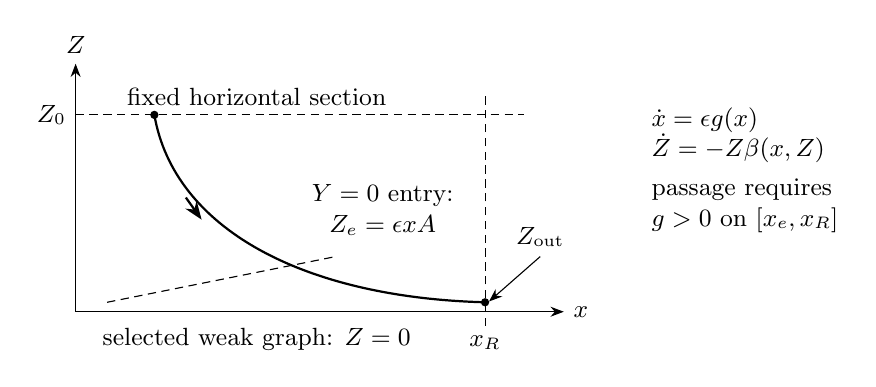
\begin{tikzpicture}[x=1cm,y=1cm,>=Stealth,font=\small]
 \draw[->] (0,0)--(6.2,0) node[right] {$x$};
 \draw[->] (0,0)--(0,3.15) node[above] {$Z$};
 \draw[densely dashed] (0,2.5)--(5.7,2.5);
 \node[above] at (2.3,2.5) {fixed horizontal section};
 \node[left] at (0,2.5) {$Z_0$};
 \draw[densely dashed] (0.4,0.12)--(3.3,0.7);
 \node[above,align=center] at (3.9,0.85)
       {$Y=0$ entry:\\$Z_e=\epsilon xA$};
 \draw[densely dashed] (5.2,-0.18)--(5.2,2.8);
 \node[below] at (5.2,-0.18) {$x_R$};
 \draw[thick] (1,2.5)..controls(1.25,1.05)and(2.9,0.18)..(5.2,0.12);
 \draw[->,thick] (1.4,1.45)--(1.6,1.17);
 \fill (1,2.5) circle(1.5pt);
 \fill (5.2,0.12) circle(1.5pt);
 \draw[->,thin] (5.9,0.7) node[above] {$Z_{\rm out}$} --(5.25,0.13);
 \node[below] at (2.3,-0.08) {selected weak graph: $Z=0$};
 \node[align=left] at (8.5,1.8)
       {$\dot x=\epsilon g(x)$\\$\dot Z=-Z\beta(x,Z)$\\[3pt]
        passage requires\\$g>0$ on $[x_e,x_R]$};
\end{tikzpicture}
\caption{Section conventions in the straightened lower phase chart
(schematic). The solid curve illustrates a forward normally contracting
passage on its positive slow component; dashed lines are transverse
sections, not invariant manifolds. A fixed horizontal entry and the
finite $Y=0$ entry have different normal sizes. Their labels are retained
in the estimates. The drawing assumes separated entry and exit; it does
not represent a passage through a scalar root or a collision of sections.}
\label{rw:fig:phase-sections}
\end{figure}

\subsection{An exact phase on the lower strip}

The lower strip contracts in the normal direction while its slow phase
moves at order $\epsilon$.  The horizontal coordinate of the
compactified chart also moves during fast contraction, so it cannot
serve as this phase.  We first project along the zero-scale fast
fibres, then correct the projection at positive scale to obtain an
exact scalar equation.  In the incoming chart put
\[
 T=(-X)^{-1},\qquad v=Y/(-X),\qquad w=v+\epsilon T=\epsilon zT,
 \qquad \frac{\dd\zeta}{\dd\xi}=-X>0.
\]
Direct substitution in the scaled original field gives
\begin{equation}\label{rw:transitions:compact-lower}
\begin{aligned}
 \dot T={}&\epsilon T[\bar B-\bar aT+(1+\epsilon\bar m)T^2]
       -(1+2\epsilon\bar m)T^2w+\bar mTw^2,\\
 \dot w={}&\epsilon^2\nu T^2+
 [-1+\epsilon\bar B+\epsilon(1+\epsilon\bar m)T^2
                  -\epsilon(\bar a+\bar c+2\nu)T]w\\
 &+[\bar c+\nu-(1+2\epsilon\bar m)T]w^2+\bar m w^3.
\end{aligned}
\end{equation}
Dots in this subsection denote $\zeta$-time. The outgoing chart is
obtained by reversing time and replacing
$(\bar a,\bar c,\nu)$ by $(-\bar a,-\bar c,-\nu)$.

Fix a small $R>0$ such that
$1\pm\bar aX+\bar BX^2>3/4$ for $0\le X\le2R$ throughout
the chosen bounded coefficient box, and put $T_R=1/R$.
All constructions below take place first on a slightly larger
$T$-interval than $[0,T_R]$.

\begin{proposition}[Lower phase]\label{rw:phase}
For each prescribed finite order $N$, there are a normal width and a
scale cutoff for which the following statements hold on common smaller
state and coefficient domains. There is an invariant graph
\begin{equation}\label{rw:transitions:weak-graph}
 w_g(T)=\epsilon^2\nu T^2H(T;\mathbf b,\epsilon),
 \qquad H(0;\mathbf b,\epsilon)=\frac1{1+\epsilon\bar B},
\end{equation}
and coordinates $(x,Z)$, with $Z=w-w_g(T)$ and $x=T$ on that graph,
in which the field is exactly
\begin{equation}\label{rw:transitions:lower-triangular}
 \dot x=\epsilon g_I(x),\qquad
 g_I(x)=xF_I(x),\qquad \dot Z=-Z\beta_I(x,Z).
\end{equation}
Their finite mixed derivatives, including the ordinary scale derivatives
used in their construction, are bounded. The normal rates satisfy
\[
 \beta_I>\beta_*,\qquad
 \beta_I+Z\partial_Z\beta_I>\beta_*,\qquad
 \beta_I(0,0)=1-\epsilon\bar B.
\]
Moreover,
\begin{equation}\label{rw:transitions:lower-factor}
\begin{aligned}
 F_I(x)={}&\bar B-\bar ax+(1+\epsilon\bar m)x^2
 -\epsilon\nu(1+2\epsilon\bar m)x^3H(x)
 +\epsilon^3\nu^2\bar m x^4H(x)^2,\\
 F_I(0)={}&\bar B,\qquad F_I'(0)=-\bar a.
\end{aligned}
\end{equation}
Thus $F_I''>1$ after the scale cutoff is reduced, and $F_I$ has a
positive margin near the fixed exit $x_R=T_R$.
In the derivative convention of this section,
$\beta_I(x,0)=1+O_{C^N}(\epsilon)$.
Ordinary differentiation with respect to $\epsilon$ may remove the
factor $\epsilon$ in this last estimate.
\end{proposition}

\begin{proof}
At $\epsilon=0$ the field is
\[
 \dot T=Tw(\bar m w-T),\qquad
 \dot w=w[-1+(\bar c+\nu-T)w+\bar m w^2].
\]
Choose the normal width small enough that the bracket in the second
equation is less than $-2\beta_*$, and that the variation of $T$ before
normal contraction is contained in the larger $T$-interval. Extend the
field smoothly outside this larger interval, preserving $T=0$, $w=0$
and this contraction. One can do this by bounded cutoffs in the
coefficient functions multiplying their displayed factors. The extension
is used only to define a complete auxiliary flow.

Define its fast projection by
\[
 \pi_0(T,w)=\lim_{t\to\infty}T(t).
\]
The decay $|w(t)|\le C|w|e^{-2\beta_*t}$ makes $\dot T$ integrable.
The variational system has a negative normal diagonal, an integrable
horizontal diagonal, and horizontal and coefficient couplings containing
$w(t)$. Variation of constants bounds horizontal variations and gives
normal decay. Higher normal forcings and derivatives of $\dot T$ retain
a normal state or lower normal variation; induction bounds them by
$C(1+t)^Me^{-\beta_*t}$, including frozen coefficient derivatives. Hence
\begin{equation}\label{rw:transitions:zero-phase}
 \pi_0(T,0)=T,\qquad \pi_0(0,w)=0,\qquad
 \pi_0-T=O\bigl(Tw(|T|+|w|)\bigr),\qquad
 \partial_T\pi_0>1/2.
\end{equation}
The order follows by integrating $Tw(\bar m w-T)$, whose factors the
flow preserves. A smaller normal width gives the derivative margin.

Use $\chi=\pi_0(T,w)$ as base coordinate. Its velocity vanishes
identically when $\epsilon=0$, and on $\chi=0$. Successive Hadamard
integration therefore writes it as $\epsilon\chi A$. Its time-one
state derivative in the base direction is $1+O(\epsilon)$, whereas
the normal multiplier is at most $e^{-\beta_*}+O(\epsilon)$.
The time-one graph transform is consequently a contraction on a small
set of graphs over the extended base. For its $k$th state derivative
the coefficient of the highest graph derivative is bounded by
\[
 e^{-\beta_*}(1+C|\epsilon|)^k+C|\epsilon|<1
\]
once $k$ is fixed and the scale cutoff is small enough. The lower
terms depend on lower graph derivatives. This proves convergence in
$C^k$ by induction, applied also to differences of consecutive iterates.

Ordinary $\epsilon$ differentiation introduces an $O(1)$ base
shear.  Order the induction first by total order, then by the number
of coefficient derivatives.  The highest unknown retains the same
contracting multiplier, and forcing of the same total order involves
fewer coefficient derivatives.  The scalar
variational equations give
\begin{equation}\label{rw:transitions:slow-variations}
 |D^\alpha\phi_t|\le C_\alpha(1+|t|)^{m_\alpha}
                       e^{C_\alpha|\epsilon||t|}.
\end{equation}
An ordinary scale derivative adds the time factor in the
variation-of-constants integral; iteration gives the displayed bound.
Normal contraction absorbs all finite polynomial factors. The graph
transform therefore converges with the prescribed mixed smoothness,
and uniqueness makes its graph invariant under the whole flow.

Return to the original $T$ parametrization. The graph is zero at
$\nu=0$ and at $\epsilon=0$. Its first ordinary $\epsilon$
derivative is also zero at $\epsilon=0$: differentiation of the
invariance equation has zero forcing there, because the independent
forcing in \eqref{rw:transitions:compact-lower} begins with
$\epsilon^2\nu T^2$. Finally its value and first $T$ derivative at
$T=0$ vanish. The point $(0,0)$ is invariant, and its weak and normal
linear eigendirections are distinct. These statements give the five
factors $\epsilon^2\nu T^2$ by finite-order Hadamard integration.
To retain order $N+2$ afterwards, construct the graph with at least
$N+7$ joint derivatives. Comparing the $T^2$ coefficient in its
invariance equation gives
\[
 2\epsilon\bar B\,w_{g,2}
   =\epsilon^2\nu+(-1+\epsilon\bar B)w_{g,2},
\]
which proves the exact value of $H(0)$.

Subtract the graph and reparametrize the base so that its coordinate
$x_0$ agrees with $T$ on the graph. In these coordinates
\[
 \dot x_0=\epsilon a(x_0)+\epsilon Z\Gamma(x_0,Z),
 \qquad \dot Z=-Z\widetilde\beta(x_0,Z).
\]
The factor $\epsilon$ survives because the zero-scale coordinate is
$\pi_0$; invariance of $T=0$ also makes $\Gamma(0,Z)=0$.
Let $\phi_t$ be the complete scalar flow of $\dot x_0=\epsilon a(x_0)$.
Set
\[
 x=\lim_{t\to\infty}\phi_{-t}(x_0(t)).
\]
Indeed,
\[
 \frac{\dd}{\dd t}\phi_{-t}(x_0(t))
   =\epsilon D\phi_{-t}(x_0(t))Z(t)\Gamma(x_0(t),Z(t)),
\]
and each selected derivative is bounded by
$C(1+t)^M e^{-(\beta_*-C_N|\epsilon|)t}$, by
\eqref{rw:transitions:slow-variations}. Reduce the scale cutoff so
that $C_N|\epsilon|<\beta_*/8$ for all the finitely many variational
products used below; the majorants are then integrable. The limit is a
coordinate with the prescribed finite smoothness, equals $x_0$ on
the graph, and differs from
$x_0$ by $\epsilon x_0ZO_{C^N}(1)$. The flow identity for the limit
gives $\dot x=\epsilon a(x)$ exactly. Restriction of the original
$T$ equation to the graph now yields
\eqref{rw:transitions:lower-factor}.

The normal linear eigenvalue at $T=w=0$ is exactly
$-1+\epsilon\bar B$. At zero scale its value along $w=0$ is $-1$.
Continuity, on the common compact domains and with the stated finite
jets, proves the normal estimates. Convexity follows from
\eqref{rw:transitions:lower-factor}. Finally $x_R=1/R$ and the
choice of $R$ give
$\bar B-\bar ax_R+x_R^2>3x_R^2/4$; reducing the scale cutoff
preserves a fixed positive margin there.
\end{proof}

\begin{lemma}[Sections and the actual exit]\label{rw:transitions:lower-sections}
On the fixed horizontal section $v=v_h>0$, with $v_h$ sufficiently
small, the phase input is
$t=x(T,v_h+\epsilon T)=T k(T)$, where $k>c>0$ and $t_T>c>0$.
The normal input has a positive lower bound. On the section $Y=0$
with $T$ in a fixed compact subset of $(0,T_R)$, it is instead
$w=\epsilon T$, the normal input is $\epsilon$ times a positive
bounded unit, and $x=T+O_{C^N}(\epsilon)$.

Restrict either entry to a fixed positive phase distance from $x_R$.
Its forward orbit reaches the fixed phase exit $x=x_R$ if and only if
\begin{equation}\label{rw:transitions:lower-passing}
g_I(s)>0\qquad(t\le s\le x_R).
\end{equation}
This criterion concerns the phase exit in the signed tube. Positivity
of the original central height is imposed separately after composition.
The entire transit remains in the chosen strip, and its duration
$T_f$ is at least $c/\epsilon$. Its selected finite time jets obey
\[
 |D^\alpha T_f|\le C\epsilon^{-M}(1+T_f)^M
                         e^{C_N\epsilon T_f}.
\]
\end{lemma}
\begin{proof}
Equation~\eqref{rw:transitions:zero-phase} and
$w_g=O(\epsilon^2T^2)$ give $Z>v_h/2$ on the horizontal entry and
positive-unit $Z/\epsilon$ on the finite entry. They also give the
phase margins, reversed in $q=1/T$ on fixed finite compact intervals.

The normal coordinate contracts, so it stays in the selected tube.
The scalar phase crosses exactly under \eqref{rw:transitions:lower-passing}:
an equilibrium blocks finite-time crossing, whereas positivity on the
closed interval gives a finite transit integral. The larger domain keeps
the original orbit in the unchanged field. Bounded $g_I$ and separated
sections give $T_f\ge c/\epsilon$. For the time jets apply the implicit
hitting calculation of Appendix~\ref{rw:app:relative-variations} to
$\phi_{T_f}(t)=x_R$, using \eqref{rw:transitions:slow-variations} and
the exit speed $\epsilon g_I(x_R)\ge c\epsilon$. Thus no minimum-gap
denominator is introduced.
\end{proof}

\subsection{Relative contraction and the original central height}

The exact phase reduces a passage to scalar transit and normal
contraction.  Its linear normal factor may have a divergent action,
so we first estimate the nonlinear amplitude relative to that factor.
These relative estimates remain uniform as the transit time diverges.
We then compute the rates for a moving entry and connect the output
to $X=0$, where the closing difference is measured.

\begin{proposition}[Relative normal contraction]\label{rw:relative-core}
Fix $N\ge1$ and a slightly larger state and coefficient domain on which
\begin{equation}\label{rw:relative:field}
 \dot w=q f(w;\mathbf b),\qquad
 \dot Z=-Z\beta(w,Z;\mathbf b),\qquad
 \beta,\ \beta+Z\beta_Z\ge b_*>0.
\end{equation}
Here $0<q\le1$, the coefficients and the field have bounded selected
jets through order $N+2$. The triangular field has a complete auxiliary
extension preserving these bounds and the normal margins.
The selected derivatives are ordinary normal-input, slow-entry and
coefficient derivatives and, when $q=\epsilon$, Euler scale derivatives.
Suppose that their scalar flow variations through the required order
are bounded by
\begin{equation}\label{rw:relative:slow-growth}
 C_N(1+t)^{M_N}e^{c_N\varpi t}.
\end{equation}
Choose the normal neighborhood and slow width so that
$c_N\varpi<b_*/8$, increasing $c_N$ first to cover all products of
variations through this order. At the fixed slow exit suppose that its
velocity has magnitude at least $cq$ and that its hitting time satisfies
\begin{equation}\label{rw:relative:time-jets}
 |D^\alpha T|\le C_Nq^{-M_N}(1+T)^{M_N}e^{c_N\varpi T},
 \qquad 1\le|\alpha|\le N+1.
\end{equation}
If $q$ tends to zero, also require $T\ge c/q$.

For every actual passing orbit and signed normal input $z$ in a fixed
small interval, its normal output is
\begin{equation}\label{rw:relative:output}
 G(z)=Lz e^{j(z)},\qquad
 L=\exp\left[-\int_0^T\beta(w(t),0;\mathbf b)\,\dd t\right]>0,
 \qquad j(0)=0.
\end{equation}
The selected jets of $j$ through order $N$ are bounded uniformly in
$T$ and the minimum positive slow gap. The jets of $L$ and $G$ have
absolute bounds $C_Ne^{-b_*T/4}$, after increasing $C_N$; this assertion
includes mixed normal-input derivatives of $G$. In particular, normal
input zero is included in the relative statement.

If $z_*(\mathbf b)$ has bounded selected jets and stays in the smaller
normal interval, then
\begin{equation}\label{rw:relative:difference}
 G(z_*+u)-G(z_*)=G'(z_*)u e^{r(u)},\qquad
 r(0)=0,\qquad \|r\|_{N}\le C_N,
\end{equation}
on a fixed smaller $u$ interval. At a slow-root loss of the exit,
with entry and exit sections remaining separated and $T\to\infty$,
define the relative
integral along the complete auxiliary flow up to infinite time and
extend $L$ and the absolute output by zero. These definitions give
extensions of class $C^N$ in the selected ordinary variables through
each such boundary, with the stated Euler bounds.
At $\epsilon=0$ this assertion uses the Euler scale class just specified,
not ordinary scale derivatives. They do not assign a physical passage
to a nonpassing parameter.
\end{proposition}

\begin{proof}
Write $g(w,Z)=Z\beta(w,Z)$. The normal equation and its first variation
give
\[
 |Z(t;z)|\le |z|e^{-b_*t},\qquad
 G_t'(z)=\exp\left[-\int_0^t g_Z(w(s),Z(s;z))\,\dd s\right]>0.
\]
Subtracting the invariant-graph rate leaves the nonlinear defect
\begin{equation}\label{rw:relative:integral}
 j(z)=-\int_0^T\mathcal I(t,z)\,\dd t,\qquad
 \mathcal I=\beta(w(t),Z(t;z))-\beta(w(t),0)
 =Z(t;z)\int_0^1\beta_Z(w(t),sZ(t;z))\,\dd s.
\end{equation}
The mixed normal induction in Appendix~\ref{rw:app:relative-variations} gives
\begin{equation}\label{rw:relative:majorant}
 |D^\alpha\mathcal I(t,z)|
 \le C_N(1+t)^{M_N}e^{-(b_*-c_N\varpi)t},\qquad |\alpha|\le N.
\end{equation}
Its endpoint calculation uses \eqref{rw:relative:time-jets} and, for
$q\to0$, $q^{-1}\le T/c$. It bounds the relative jets and proves the
absolute estimates for $G,L$ separately.

For the difference formula, use instead
\[
 \log\frac{G'(z)}{L}
 =-\int_0^T[g_Z(w(t),Z(t;z))-\beta(w(t),0)]\,\dd t.
\]
The same majorant makes
$G'(z_*+\theta u)/G'(z_*)$ a positive unit with bounded
selected jets. Integrate it for $0\le\theta\le1$ and take its logarithm
to obtain \eqref{rw:relative:difference}.

Persistence of a finite transverse exit forces $T\to\infty$ at the
specified separated-section slow-root boundary. The appendix proves the
relative extension by differentiated tails and the absolute zero extension.
Entry--exit collision, where $T\to0$, is excluded.
\end{proof}

For the lower phase, take $q=\epsilon$ and
$\varpi=O(\epsilon)$; separated sections give $T\ge c/\epsilon$.
For an upper angular passage, take $q=1$ and use a small angular
width to obtain normal domination.  In both cases the estimates allow
independently vanishing slow gaps.  The action $-\log L$ remains in
the linear factor, with no bound required for it or its gap derivatives.

\begin{corollary}[Continuity of the relative passage]
\label{rw:transitions:relative-continuity}
Consider a family satisfying Proposition~\ref{rw:relative-core}
with common domains, margins and finite-order bounds. Suppose its
auxiliary trajectories and reserved mixed jets converge on bounded
time intervals, and its exit times converge to the corresponding
finite exit or to infinity. Then the relative amplitude and the
logarithm of the normal derivative divided by its linear factor
converge in the selected finite norms, including at a lost exit.
No derivative of the divergent linear action is included.
\end{corollary}
\begin{proof}
Use \eqref{rw:relative:majorant} and the differentiated endpoint bound
\eqref{rw:app:endpoint-term}: pass to the limit on a fixed time interval,
then send its endpoint to infinity. At a finite exit, transversality
also gives convergence of the time jets.
\end{proof}

\begin{lemma}[A moving slow entry]\label{rw:transitions:moving-rate}
In Proposition~\ref{rw:relative-core}, fix a normal input $Z_0>0$ and
the exit $v_R$. Let the slow entry $v$ vary with
$f(s)>0$ on the whole interval $[v,v_R]$. With
$\beta_0(s)=\beta(s,0)$, the actual output is
\begin{equation}\label{rw:relative:moving-output}
 G(v)=Z_0\exp\left[-q^{-1}\int_v^{v_R}
                    \frac{\beta_0(s)}{f(s)}\,\dd s+j(v)\right].
\end{equation}
The relative function $j$ has the selected jets of the preceding
proposition, with $v$ counted as an ordinary input. Put
\begin{equation}\label{rw:relative:rates}
 N_0=\beta_0+qf j',\qquad
 A_0=N_0-qf'+qf\frac{N_0'}{N_0}.
\end{equation}
Where $N_0\ge n_*>0$,
\[
 \frac{G'}G=\frac{N_0}{qf},\qquad
 \frac{G''}{G'}=\frac{A_0}{qf}.
\]
For a regular change $v=v(t)$, $v'\ne0$, the latter formula becomes
\begin{equation}\label{rw:relative:curvature-rate}
 \frac{(G\circ v)''}{(G\circ v)'}
 =\frac{A_0v'+qf\,v''/v'}{qf}.
\end{equation}
Thus bounds through order $k$ for $A_0$ use $k+2$ entry derivatives
of $j$, and the numerator after a change of input uses $k+2$
derivatives of that change and a bound for $1/v'$.
\end{lemma}

\begin{proof}
Separate the linear rate in \eqref{rw:relative:integral} and logarithmically
differentiate; the chain rule gives \eqref{rw:relative:curvature-rate}.
The denominators $N_0,v'$ require the stated margins and derivative
orders. The transit integral uses $f>0$ along the whole path.
\end{proof}

\begin{lemma}[The fixed phase exit in original coordinates]
\label{rw:transitions:curved-exit}
Choose a fixed lower phase exit away from $T=0$. Use the compact lower
coordinates and their inverse from Proposition~\ref{rw:phase}. At this
exit write $Z=Z_{\rm out}$ and set $\eta=Z_{\rm out}/\epsilon$.
On a fixed sufficiently small signed $\eta$ interval, passage from this
curved exit to a fixed original section $|X|=R$ has bounded ordinary
$\eta$, coefficient and Euler scale jets of every prescribed finite
order, provided the phase construction retains these orders. After
orienting the normal coordinate positively, the deviation from the
same weak reference on $|X|=R$ is
\begin{equation}\label{rw:relative:curved-section}
 W=\eta u_c(\eta,\mathbf b,\epsilon),\qquad
 u_c\ge c_*>0,
\end{equation}
with bounded jets of $\log u_c$. The original horizontal displacement
at the curved exit is $O_{C^N}(\epsilon\eta)$.
\end{lemma}

\begin{proof}
At the fixed phase exit, inversion gives $T=T_b+ZO_{C^N}(1)$,
with $T_b>c>0$; hence $X=-1/T$ moves by $ZO_{C^N}(1)$.
The exact compact relation is $w=\epsilon zT$ and
$w=\epsilon^2\nu T^2H(T)+Z$. Hence
\[
 z=\epsilon\nu TH(T)+\frac{Z}{\epsilon T}.
\]
Subtract the same weak reference at the shifted $T$ and substitute
$Z=\epsilon\eta$ before differentiation. The deviation is $\eta/T$,
a positive bounded unit times $\eta$.

Put $|X|=R+\epsilon\xi$. Its graph equation has bounded finite jets
on a fixed $(\xi,\eta)$ box, since $R>0$ and the horizontal denominator
has a positive margin. The section moves by $\xi=O(\eta)$; finite
ODE dependence and the positive normal derivative give
\eqref{rw:relative:curved-section} and the inverse bounds.

For an actual lower slow passage, retain a fixed final piece with
time at least $c/\epsilon$. Proposition~\ref{rw:relative-core} then
implies that $Z_{\rm out}/\epsilon$ and all selected jets are
exponentially small. Thus the actual output lies in the signed box
used for this construction.
\end{proof}

\begin{proposition}[The Gaussian central connection]
\label{rw:transitions:central-core}
Fix $0<R_0<R_1$ and a compact coefficient box such that
\[
 F_+(X)=1+\bar aX+\bar BX^2\ge f_*>0
 \quad(0\le X\le R_1).
\]
Let $R\in[R_0,R_1]$ be fixed independently of the section input, with
bounded selected coefficient and Euler jets if it varies with parameters.
Continue the chosen weak reference from
$z_b(R)=\epsilon\nu h_b$, where $h_b$ has bounded selected jets.
For sufficiently small $\epsilon>0$ and $|\nu|$, this continuation
exists on $0\le X\le R$ and satisfies
\begin{equation}\label{rw:relative:reference-weight}
 |z_b(X)|\le\frac{C\epsilon|\nu|}{X+\sqrt\epsilon},\qquad
 |D^\alpha z_b(Ry)|\le
       \frac{C_N\epsilon}{Ry+\sqrt\epsilon},\quad |\alpha|\le N.
\end{equation}
Here $0\le y\le1$ is fixed when taking coefficient or Euler
derivatives. The factor $\nu$ remains whenever no $\nu$ derivative
is taken.

For signed input $z(R)=z_b(R)+W$ in a fixed small interval, its
central height is
\begin{equation}\label{rw:relative:central-output}
 z(0)=s_b+e^{-S_c/\epsilon}a_cW e^{j_c(W)},\qquad
 s_b=z_b(0),\qquad S_c=\int_0^R\frac{X}{F_+(X)}\,\dd X>0.
\end{equation}
The positive factors $a_c,a_c^{-1}$ and the selected jets of
$\log a_c,j_c$ through order $N$ are bounded, and $j_c(0)=0$.
Ordinary $W$ derivatives are included. Composing with
\eqref{rw:relative:curved-section} gives the same statement with
$W$ replaced by $\eta$ and with adjusted positive units.
All reference choices are independent of the moving section input.
\end{proposition}

\begin{proof}
The exact original graph equation is
\begin{equation}\label{rw:relative:core-field}
 \frac{\dd z}{\dd X}=\mathfrak f(X,z)
 =\frac{(X/\epsilon)z+\bar c z(z-1)+\nu(1-z)^2}{D(X,z)},
 \quad
 D=F_++\epsilon\bar m-(1+2\epsilon\bar m)z
                         +\epsilon\bar m z^2.
\end{equation}
Its denominator stays positive on a fixed small signed tube.
The weighted Gaussian kernel and Volterra estimates in
Appendix~\ref{rw:app:relative-core} give
\eqref{rw:relative:reference-weight}, including its selected mixed jets.

Put $v=z-z_b$. Exact Taylor division gives
\[
 v_X=a(X)v+B_c(X,v)v^2,\quad
 a(X)=\frac{X}{\epsilon F_+(X)}+a_r(X),\quad
 |a_r|\le C,\quad
 |\partial_v^jB_c|\le C_j(X/\epsilon+1).
\]
These bounds include selected coefficient and Euler jets because
\eqref{rw:relative:reference-weight} controls $(X/\epsilon)z_b$.
Set $E(X)=\exp[-\int_X^R a(s)\,\dd s]$ and solve directly for the
relative logarithm:
\begin{equation}\label{rw:relative:normalized-volterra}
 Q(X)=-W\int_X^R B_c(s,WE(s)e^{Q(s)})E(s)e^{Q(s)}\,\dd s.
\end{equation}
The weighted kernel bound \eqref{rw:app:normalized-kernel-bound} and
the differentiated contraction proof in Appendix~\ref{rw:app:relative-core}
give $\|Q\|_\infty\le C|W|$ and bounded selected jets on a fixed
small $W$ interval, including zero. Thus $v(X)=WE(X)e^{Q(X)}$.
Set
$a_c=\exp[-\int_0^R a_r]$ and $j_c(W)=Q(0,W)$.
This proves \eqref{rw:relative:central-output}, retaining the exponentially
small factor in $E$ throughout.
\end{proof}

The Gaussian layer is controlled by the weighted reference estimate;
ordinary high-order $X$ derivatives there may be unbounded.  All
derivatives of the finitely smooth phase and reference are taken on
their real parameter domains.  The signed construction supplies the
estimates and coefficient comparisons, and its physical restriction
consists of positive-height original trajectories with finite
transverse passages.
For the incoming core, apply the same construction after reflection
with $(\bar a,\bar c,\nu)$ replaced by
$(-\bar a,-\bar c,-\nu)$.

\subsection{Simple roots, quadratic passages and the cubic boundary}

The form of the lower transition depends on which root controls its
transit.  A separated simple root gives a power law, while a quadratic
minimum is described by its full transit integral.  At the horizontal
end a positive $\bar B$ gives an exact invariant-axis exponent; as
$\bar B=\bar a=0$ is approached, we retain the whole slow factor
$xF_I(x)$ to avoid division by the vanishing coefficients.  Each
representation ends at the fixed phase section of
Lemma~\ref{rw:transitions:lower-sections} and then uses the same
central connection.

\begin{proposition}[Lower preparations]\label{rw:lower-preparation}
Fix a finite derivative order and a compact set of the indicated data.
The following representations hold on common auxiliary domains and on
the actual passing portions specified below.

\begin{enumerate}[label=(\roman*),leftmargin=*]
\item Suppose the first positive root $q_0$ of
$1-\bar a q+\bar Bq^2$ is simple, with
$\Delta=-\partial_q(1-\bar a q+\bar Bq^2)|_{q=q_0}>0$.
Assume $q_0$ and $\Delta$ have positive upper and lower bounds.
There is an actual strong intersection $\widehat q=q_0+O(\epsilon)$
on $Y=0$ and a regular power coordinate
$t=\chi(\widehat q-q)$, where $\chi(0)=0$ and $\chi'>c>0$.
On its passing side $t>0$ the central output is
\begin{equation}\label{rw:transitions:finite-power}
 L_-(q)=s_-+D_-(t),\qquad
 D_-(t)=K_-t^{h_-/\epsilon}e^{j_-(t)},\qquad j_-(0)=0.
\end{equation}
Here $h_->c>0$, $h_-=q_0/\Delta+O(\epsilon)$, $K_->0$,
and $j_-$ has bounded ordinary input and mixed coefficient and
Euler-scale derivatives through the prescribed order.
On this compact simple-root block the derivatives of
$\epsilon\log K_-$ in the coefficients and Euler scale are bounded.
The reflected outgoing preparation has the same properties.

\item Near an interior double root of $F_I$, there are an increasing
regular coordinate $u$ and a positive bounded time change for which
the weak equation is
\begin{equation}\label{rw:transitions:lower-morse}
 u'=\epsilon(\mu+u^2).
\end{equation}
The complete interval to the selected right exit must satisfy
$\mu+s^2>0$. The normal equation retains a fixed contracting margin.
The relative amplitude and the absolute output have the finite-order
extensions of Proposition~\ref{rw:relative-core}, without any bound
on $\epsilon/\mu$.

\item On a compact block $\bar B\ge B_*>0$, the fixed horizontal
entry of Lemma~\ref{rw:transitions:lower-sections} has
\begin{equation}\label{rw:transitions:horizontal-power}
 D_-(t)=K_-t^{h_I/\epsilon}e^{P_-(t)/\epsilon},\qquad
 h_I=\frac{1-\epsilon\bar B}{\bar B},\qquad P_-(0)=0.
\end{equation}
The selected finite jets of $P_-$ are bounded, including at $t=0$.
Its domain is the positive component that connects to the fixed exit.
The reflected exponent is exactly the same at each positive scale.
All action accumulated after a fixed small horizontal section belongs
to $K_-$; its logarithm need not have bounded gap derivatives.

\item On a neighborhood of $\bar B=\bar a=0$, including both signs
of $\bar B$, write $g=g_I=xF_I(x)$. The horizontal deviation admits
\begin{equation}\label{rw:transitions:cubic-amplitude}
 D(x)=C\exp\left[-\frac1\epsilon
       \int_x^{x_R}\frac{\beta_I(s,0)}{g(s)}\,\dd s\right]
       e^{\widetilde j(x)},\qquad C>0,
\end{equation}
where the normal entry and central relative units are included in
$\widetilde j$. Its selected ordinary input and mixed jets are bounded
on the common auxiliary domain. On the actual passing component put
\begin{equation}\label{rw:transitions:cubic-rate}
 N_I=\beta_I(x,0)+\epsilon g\widetilde j',\qquad
 A_I=N_I-\epsilon g'+\epsilon g\frac{N_I'}{N_I}.
\end{equation}
Then
\[
 D'>0,\qquad \frac{D''}{D'}=\frac{A_I}{\epsilon g},\qquad
 A_I=1+O_{C^N}(\epsilon),\qquad A_I(0)=1-2\epsilon\bar B.
\]
The rate coefficients are defined and bounded across the auxiliary
nonpassing parameters; the quotient is used only where $g>0$.
\end{enumerate}
The reference value $s_-$ in these formulas is the central value of
the one fixed weak graph, independent of the input. The outgoing
reference is obtained by the fixed-field reflection convention.
No assertion about the number of closing zeros is part of this
proposition.
\end{proposition}

\begin{proof}
For a simple root, the first task is to locate the actual strong
separatrix and normalize its input.  In the phase coordinate the root
$r$ is close to $1/q_0$;
$g_I'(r)>c>0$. The strong fibre is $x=r$. On a fixed finite root
block use the original normal height coordinate
$U_0=Z/\epsilon=Tz-\epsilon\nu T^2H(T)$, which extends smoothly
through $\epsilon=0$ after substitution of $w=\epsilon Tz$.
The phase on these states satisfies $x=T+O_{C^N}(\epsilon)$.
Thus $x=r$ is a graph over $z$, with horizontal slope
$O(\epsilon)$, and intersects $z=1$ at $q=\widehat q$ with
$\widehat q=q_0+O(\epsilon)$. Its normal rate has a fixed nonzero
margin outside a smaller saddle box. It is the strong separatrix
throughout $0<z<1$ and is a barrier to the incoming passage.
The sign in \eqref{rw:transitions:lower-passing} selects
$q<\widehat q$.

Locally put $u=U_0$ and $v=x-r$. The invariant axes give
\[
 \dot u=-uA(u,v),\qquad \dot v=\epsilon vB(u,v),
 \qquad A,B>c>0.
\]
At the equilibrium their ratio is
$h=A(0,0)/B(0,0)=q_0/\Delta+O(\epsilon)$.
Let $H_o=A/B$. Normalize the axes by the regular changes
\begin{equation}\label{rw:transitions:axis-normalization}
 \frac{\dd\log U}{\dd\log u}=\frac{h}{H_o(u,0)},
 \qquad
 \frac{\dd\log V}{\dd\log v}=\frac{H_o(0,v)}h.
\end{equation}
The right sides equal one at zero. Subtracting one before integration
shows that $U/u$ and $V/v$ are positive regular units with bounded
jets and inverses. In the new coordinates the orbital coefficient is
$h^2H_o(u,v)/(H_o(u,0)H_o(0,v))$. It equals $h$ on both axes.
Two Hadamard divisions therefore give
\begin{equation}\label{rw:transitions:large-ratio-equation}
 \frac{\dd U}{\dd V}
 =-\frac h\epsilon\frac UV-\frac{U^2}\epsilon R(U,V).
\end{equation}
The finite jets of $R$ are bounded uniformly. To obtain final order
$N$, use the phase and axis constructions two orders higher for these
two divisions, and retain another two orders for the connections and
inverses. Together with Proposition~\ref{rw:phase}, a graph order
$N+11$ suffices for this argument. Only finitely many orders are used.

Fix small positive sections $U=U_*$ and $V=V_*$ and take
$0<t<t_0<V_*/2$. The reciprocal equation gives the exact passage
\begin{equation}\label{rw:transitions:reciprocal-lower}
 \mathscr D(t)=
 \frac{U_*(t/V_*)^{h/\epsilon}}
 {1+(U_*/\epsilon)t^{h/\epsilon}
       \int_t^{V_*}s^{-h/\epsilon}R(U(s),s)\,\dd s}.
\end{equation}
The integral retains the dependence of $R$ on the solution $U$.
Set $V=t e^{\epsilon\theta}$ and
$T_f=\epsilon^{-1}\log(V_*/t)$. The denominator is $1+U_*tI$, where
\[
 I=\int_0^{T_f}e^{-(h-\epsilon)\theta}
       R(U(\theta),t e^{\epsilon\theta})\,\dd\theta,
 \qquad U_\theta=-U[h+UVR(U,V)].
\]
Here $U$ contracts uniformly and the explicit scalar flow
$V=te^{\epsilon\theta}$ satisfies \eqref{rw:relative:slow-growth}
with $\varpi=O(\epsilon)$. The mixed normal induction of
Appendix~\ref{rw:app:relative-variations} bounds the differentiated
integrands, with their additional weight $e^{-(h-\epsilon)\theta}$, by
$C(1+\theta)^M e^{-(h_*-C_N\epsilon)\theta}$.
Extend $R$ boundedly beyond $V_*$ while retaining contraction.
The infinite integral has bounded ordinary and mixed jets. The finite
tail and its endpoint terms are bounded by finite sums
$C\epsilon^{-a}t^{-b}(1+|\log(t/V_*)|)^M(t/V_*)^{h/\epsilon-1}$.
Half the exponent absorbs the input powers and logarithms, and
$t/V_*<1/2$ absorbs the inverse scale powers. Thus the selected jets
extend at $t=0$. Reducing $t_0$ makes the denominator positive and
$j=-\log(1+U_*tI)$ has bounded jets with $j(0)=0$.

The transverse connection from $z=1$ to the local fast section has
bounded jets and inverse jets in the original finite-height coordinates;
composing its input with $V$ gives the regular deficit $t$.
The remaining leg stays away from the simple root and reaches the fixed
phase exit. Its input-independent linear contraction belongs to $K_-$;
its relative unit is controlled by Proposition~\ref{rw:relative-core}
and Lemma~\ref{rw:transitions:curved-exit}, followed by
Proposition~\ref{rw:transitions:central-core}. The large power absorbs
the finite ordinary derivative losses, so composition preserves the
relative jets. Absorb the unit's value at zero into $K_-$.
On this simple-root compact block the remaining linear action is an
integral over intervals whose slow denominators have positive margins.
It follows that $\epsilon\log K_-$ has bounded coefficient and
Euler-scale jets. This proves (i), including the fixed central reference.

For (ii), let $x_0$ be the minimum of $F_I$ near the double root.
It is interior and bounded away from zero. Write
\[
 F_I(x)=\mu+(x-x_0)^2a(x),\qquad
 a(x)=\int_0^1(1-s)F_I''(x_0+s(x-x_0))\,\dd s>c.
\]
The increasing Morse coordinate $u=(x-x_0)\sqrt{a(x)}$ is regular.
Its velocity is $\epsilon(\mu+u^2)$ times the bounded positive
unit $x\partial_xu$. Dividing time by this unit gives
\eqref{rw:transitions:lower-morse}. The normal contraction remains uniformly positive.
Apply Proposition~\ref{rw:relative-core} on the whole passing interval,
with the fixed exit margin. Crossing the minimum requires $\mu>0$;
for $\mu\le0$ a right-hand entry must exceed $\sqrt{-\mu}$.
The same fixed phase and central connections complete the passage.

For (iii), choose $x_h>0$ small enough that $F_I>c>0$ on
$[0,x_h]$ throughout the positive-$\bar B$ block. Since
$\beta_I(0,0)=1-\epsilon\bar B$ and $F_I(0)=\bar B$,
\begin{equation}\label{rw:transitions:horizontal-division}
 \frac{\beta_I(x,0)}{xF_I(x)}=\frac{h_I}{x}+q_0(x)
\end{equation}
with $q_0$ having bounded finite jets at zero; subtraction of the
constant value and one Hadamard division prove this statement.
The exact normal integral from the fixed horizontal entry is
\[
 Z_{\rm out}=Z_e(t)
 \exp\left[-\frac1\epsilon\int_t^{x_R}
       \frac{\beta_I(s,0)}{sF_I(s)}\,\dd s\right]e^{j(t)}.
\]
The factor $Z_e$ is bounded away from zero for this section.
Separate the integral at $x_h$ and use
\eqref{rw:transitions:horizontal-division}. After the central relative
unit is included, its input-dependent logarithm multiplied by
$\epsilon$ is
\[
 P_-(t)=\int_0^t q_0(s)\,\dd s
 +\epsilon\log\frac{Z_e(t)}{Z_e(0)}
 +\epsilon\bigl(\widetilde j(t)-\widetilde j(0)\bigr).
\]
All its required jets are bounded by the relative estimates, even
when a later slow exit is lost. For each passing parameter the
input-independent action on $[x_h,x_R]$ belongs to $K_-$.
A later loss of passage gives the absolute zero extension of
Proposition~\ref{rw:relative-core}; $\log K_-$ may still have
unbounded gap derivatives there.
Reflection fixes $\bar B$ and $\epsilon$, so $h_I$ agrees exactly
on the two sides. If a separately normalized power input is needed,
$t\exp(h_I^{-1}\int_0^t q_0)$ absorbs the pure weak-axis action;
it and its inverse have bounded jets. In a common actual input the
scaled remainder $P_-$ is the appropriate representation.

For (iv), retain the undistributed slow factor $g=xF_I$.
The exact linear normal integral and the relative amplitudes give
\eqref{rw:transitions:cubic-amplitude}; the fixed horizontal normal
input is a positive unit, so its logarithm can be included in
$\widetilde j$. Use \eqref{rw:relative:rates} with
$(q,f,j)=(\epsilon,g,\widetilde j)$ and
$N_I=1+O(\epsilon)>0$ to obtain the rate formula.
At zero, $g(0)=0$ and $g'(0)=\bar B$; hence
$N_I(0)=1-\epsilon\bar B$ and
$A_I(0)=1-2\epsilon\bar B$ exactly. The finite jets of the
relative amplitude and of $g,\beta_I$ give those of $N_I,A_I$.
To retain a rate coefficient through order $N$, retain the primitive
through order $N+2$ before differentiating.  The construction remains
regular when $\bar B$, $\bar a$ or a slow gap vanishes, since these
factors have not been divided out.  The values and logarithmic
derivatives of $D$ are used on the passing component
\eqref{rw:transitions:lower-passing}; its relative coefficients and
absolute zero extension are defined on the larger auxiliary domain.
\end{proof}

\begin{remark}[The choice of section matters]
The exponent in \eqref{rw:transitions:horizontal-power} belongs to a
fixed positive horizontal fast section. The finite section $Y=0$ has
normal input $\epsilon$ times a unit on finite $T$-intervals; at
$T=0$ it has an additional vanishing $T$ factor. Thus extending that
section to the horizontal boundary does not preserve the displayed
power without accounting for its input factor. Likewise an arbitrary
regular substitution $t\mapsto tk(t)$ contributes
$(h/\epsilon)\log k(t)$ to an unscaled power logarithm.
The normalized input of (i) absorbs this action; the common-input
formula (iii) records it in $P/\epsilon$.
\end{remark}

\subsection{A finite upper saddle near ratio one}\label{rw:upper-resonance}

We first treat the finite hyperbolic saddle, then the repeated and weak
ends at infinity.  Near ratio one, expanding a power in the ratio
would lose uniformity when its logarithmic input is large.  Instead
we keep the exact compensator.  The original field is affine at zero
scale, so its nonlinear orbital remainder has a factor $\epsilon$,
which persists in the compensator and curvature estimates.  Fix a compact
interval $0<m_*\le\bar m\le m^*$, bounded remaining coefficients and a
small neighborhood on which its eigenvalue ratio satisfies
$|r-1|\le1/64$. The ratio used below is the actual ratio of the original
field. Dividing \eqref{rw:geometry:upper-field} by $Y+\epsilon>0$ gives
\begin{equation}\label{rw:upper:divided-field}
 \dot X=\frac{Y(\bar mY-1)+\epsilon(\bar BX^2+\bar aX)}{Y+\epsilon},
 \qquad
 \dot Y=X+\bar cY+\frac{\nu Y^2}{Y+\epsilon}.
\end{equation}
At $\epsilon=0$ this is an affine field. Its saddle is
$(-\bar d/\bar m,1/\bar m)$, where $\bar d=\bar c+\nu$, and its two
eigenvalues have opposite signs separated from zero. The implicit
function theorem gives the perturbed saddle and its eigendirections on
a common analytic coefficient neighborhood. Write its eigenvalues as
$\lambda_u>0>\lambda_s$ and set $r=-\lambda_s/\lambda_u$.

To bound the analytic jets near this finite saddle, choose a complex
neighborhood whose real part lies in $Y>Y_s/2>0$.  On a sufficiently
small such neighborhood, $Y+\epsilon$ stays away from zero.  In linear
eigenvector coordinates the stable and unstable graph equations have
coefficient denominators $n\lambda_u-\lambda_s$ and
$\lambda_u-n\lambda_s$, respectively. Their absolute values are at
least $c(n+1)$ for $n\ge1$ on a smaller complex coefficient disk.
The nonlinear part of \eqref{rw:upper:divided-field} is $\epsilon$
times an analytic function. On a sufficiently small state disk the
coefficient recursion is therefore a contraction in the norm
$\sum|a_n|\delta^n$; the factor $(n+1)^{-1}$ absorbs the derivative
index in the graph equation. This constructs both axes on one disk,
with their nonlinear parts divisible by $\epsilon$. Cauchy estimates
on smaller disks give any prescribed finite state and coefficient jets,
including Euler scale jets of the quotient by $\epsilon$.

Straighten these axes, orient their coordinates $U,V$ positively in the
quadrant of the local returning arc, and write the orbital equation as
$V_U=-(V/U)H(U,V)$, with $H(0,0)=r>0$. Separate positive changes on the
two axes, obtained by integrating
$d\log\widetilde U/d\log U=H(U,0)/r$ and
$d\log\widetilde V/d\log V=r/H(0,V)$, make the orbital coefficient
constant on each axis. Its difference from $r$ is then divisible by
$UV$. Dropping the tildes gives
\begin{equation}\label{rw:upper:axis-equation}
 \frac{dV}{dU}=-r\frac VU-V^2R(U,V),\qquad R=\epsilon\widetilde R,
\end{equation}
where $\widetilde R$ has common analytic bounds.  The local maps below
follow this positive quadrant.  To obtain the complete upper path,
they will be composed with its two regular connecting arcs.

The coordinates can be chosen to preserve the reversible component
$\bar a=\bar c=\nu=0$ exactly. Indeed, with $Y_s=1/\bar m$, put
\begin{gather*}
 W(Y)=\left(\frac{Y+\epsilon}{Y_s+\epsilon}\right)^{-2\epsilon\bar B},
 \qquad
 I(Y)=\int_{Y_s}^Y\frac{2s(\bar ms-1)}{s+\epsilon}W(s)\,ds.
\end{gather*}
Direct differentiation gives the first integral $WX^2-I$.
Writing $I=(Y-Y_s)^2J$ yields
$J(Y_s)=\bar m/(1+\epsilon\bar m)>0$. Thus
$\eta=(Y-Y_s)\sqrt{J/\bar m}$,
$\zeta=\sqrt{W/\bar m}X$ and
$U=-(\eta+\zeta)/2$, $V=-(\eta-\zeta)/2$ transform that integral to
$-4\bar mUV$. Extend these analytic coordinates to the coefficient
neighborhood before straightening the perturbed axes. The subsequent
axis changes are the identity on this component; there $r=1$ and
$R=0$ exactly.  This local first integral supplies the normalization
on the reversible component.

\begin{proposition}[The uniform resonant passage]\label{rw:upper:prepared-map}
After choosing common small local sections and positive coordinates on
them, the passage from $(t,1)$ to $(1,v)$ has the form
\begin{equation}\label{rw:upper:comp-map}
 v=t^r e^{w(t)},\qquad
 w=-\sigma t\omega(t;r-1)+R_w(t),\qquad
 \omega(t;\kappa)=\int_0^{\log(1/t)}e^{-\kappa s}\,ds.
\end{equation}
For each prescribed finite integer $N$, the neighborhoods can be chosen
so that, with $D=t\partial_t$,
\begin{equation}\label{rw:upper:remainder}
 |D^i\partial_{\mathbf b}^{\alpha}E_\epsilon^jR_w|
 \le C_N\epsilon t^{7/4},\qquad i+|\alpha|+j\le N,
 \qquad 0<t<e^{-6}.
\end{equation}
Ratio derivatives may also be included, counting towards the same total
order. The coefficients satisfy $\sigma=O(\epsilon)$ in these norms.
In particular $N=6$ supplies four input Euler derivatives and two
coefficient derivatives of $R_w$. The estimate places no bound on
$|(r-1)\log t|$.
\end{proposition}

\begin{proof}
First remove the nonconstant restrictions of $R$ to its axes without
dividing by $r-1$. Put $s_0=R(0,0)$ and, writing
$R(U,0)=s_0+\sum_{n\ge1}R_{n0}U^n$, set
\[
 f(U)=-\sum_{n\ge1}\frac{R_{n0}U^{n+1}}{n+1-r},\qquad
 V_1=\frac V{1+f(U)V}.
\]
A direct differentiation gives
\[
 R_1(U,V_1)=R\left(U,\frac{V_1}{1-f(U)V_1}\right)
                  +f'(U)-rf(U)/U,
 \qquad R_1(U,0)=s_0.
\]
Next set $U_1=U/(1+g(V_1)U)$, where $g(0)=g'(0)=0$ solves
\[
 g'(V)-\frac{g(V)}{rV}=\frac{R_1(0,V)-s_0}{r^2}.
\]
The new axis restriction is
$R_2(0,V)=R_1(0,V)-r^2g'(V)+rg(V)/V=s_0$.
Since $g=O(V^2)$, the previously normalized axis is unchanged.
The denominators of the two series are $n+1-r$ and $n+1-1/r$,
$n\ge1$. On $|r-1|\le1/64$ they have a fixed positive margin and
grow linearly with $n$. The changes and their inverses therefore have
uniform analytic bounds on smaller disks, and $f,g$ retain their factor
$\epsilon$. Exact division of $R_2-s_0$ by $U_1V_1$, followed by one
common positive rescaling of both sections, gives
\begin{equation}\label{rw:upper:resonant-orbit}
 V_U=-rV/U-\sigma V^2-UV^3\mathcal R(U,V),\qquad
 |\sigma|+\|\mathcal R\|\le C\epsilon.
\end{equation}
The bound includes whatever finite jets are reserved before this
construction. The two shears are also the identity on the reversible
component considered above.

The reciprocal equation before the shears has the exact integral
representation
\[
 V(U)=\frac{(t/U)^r}{1+t^r\int_t^U s^{-r}R(s,V(s))\,ds}.
\]
It proves positivity and existence on the full rectangle for small
$\epsilon$. In \eqref{rw:upper:resonant-orbit} put
$U=te^\theta$, $V=e^{-r\theta}\zeta$, and
$L=\log(1/t)$. Then, exactly,
\begin{equation}\label{rw:upper:zeta}
 \zeta_\theta=-\sigma te^{-(r-1)\theta}\zeta^2
 -t^2e^{-2(r-1)\theta}\zeta^3
        \mathcal R(te^\theta,e^{-r\theta}\zeta),\qquad \zeta(0)=1.
\end{equation}
With $\delta=1/64$ the two kernel integrals are bounded respectively by
$t^{1-\delta}L$ and $t^{2-2\delta}L$. A bootstrap on the integral
equation gives $1/2<\zeta<2$ and
$\zeta-1=O(\epsilon t^{1-\delta}(1+L))$ on $[0,L]$.
Integrating its logarithmic derivative now yields
\begin{align*}
 R_w={}&-\sigma t\int_0^L e^{-(r-1)\theta}(\zeta-1)\,d\theta\\
 &-t^2\int_0^L e^{-2(r-1)\theta}\zeta^2
                  \mathcal R(te^\theta,e^{-r\theta}\zeta)\,d\theta.
\end{align*}
Consequently $|R_w|\le C\epsilon t^{2-2\delta}(1+L)^2$.

Differentiate \eqref{rw:upper:zeta} at fixed $\theta$. Ratio derivatives
add polynomial factors in $\theta$; input Euler derivatives preserve
$te^\theta$. The highest variation has the same small-$L^1$ linear
kernel, so induction bounds it by the displayed powers of $t$ times a
fixed power of $1+L$. Endpoint rows use $DL=-1$ and retain those powers.
In the first integral for $R_w$, all variations of $\zeta-1$ retain
their first-order smallness. Therefore
\[
 |D^i\partial_{\mathbf b}^{\alpha}E_\epsilon^jR_w|
 \le C_N\epsilon t^{2-2/64}(1+L)^{M_N}.
\]
The strict exponent margin $2-2/64-7/4=7/32$ absorbs every such fixed
logarithmic power and proves \eqref{rw:upper:remainder}. Ordinary
$\epsilon$ derivatives can differentiate away the front factor
$\epsilon$ and are not covered by that displayed conclusion.
\end{proof}

The curvature formula follows from the exact identity
\[
 E:=t\frac{v''}{v'}-(r-1)=Dw+\frac{D^2w}{r+Dw}.
\]
Inserting \eqref{rw:upper:comp-map} gives
\begin{equation}\label{rw:upper:curvature}
 E=-\sigma Q+R_E,\qquad
 Q=2rt\omega(t;r-1)-(2+1/r)t,\qquad Q''=-2r^2t^{r-2}.
\end{equation}
Here $|D^i\partial_{\mathbf b}^{\alpha}E_\epsilon^jR_E|
\le C\epsilon t^{7/4}$ for $i+|\alpha|+j\le N-2$ if $N$ orders were
retained in \eqref{rw:upper:remainder}. Indeed the error in replacing
$(r+Dw)^{-1}$ by $1/r$ is a product of two first corrections, bounded
by the same $t^{2-2/64}(1+L)^M$ estimate. Thus a curvature use requiring
four Euler and two coefficient derivatives reserves $N=8$, whereas
four Euler and two coefficient derivatives of $w$ itself require
$N=6$. Since $\omega\ge\int_0^6e^{-s/64}\,ds>5$ and
$Q'=2r^2\omega-2r-2-1/r$, both $Q$ and $Q'$ are positive on
$0<t<e^{-6}$ for the stated ratio interval.  Both estimates retain
$t^{r-1}$ exactly and therefore remain valid when
$|(r-1)\log t|$ is large.

The finite connecting arcs contribute a separate regular factor. On a
small low-height segment where $|X|\ge c>0$, the denominator of
$dX/dY$ obtained from \eqref{rw:upper:divided-field} is bounded below
in modulus by $c(Y+\epsilon)$. The numerator and all its fixed $X$
and coefficient derivatives are $O(Y+\epsilon)$; Euler scale
differentiation preserves this property. The equation in $Y$ and its
finite variational equations consequently have bounded coefficients.
Comparing it with its zero-scale equation leaves only the integrable
layer carrier $\epsilon/(Y+\epsilon)$, whose integral is
$\epsilon\log(1+\delta/\epsilon)$. Beyond this segment the vector
field is regular on a compact arc. These arguments give the required
finite section and coefficient jets, with zero-scale error
$O(\epsilon(1+|\log\epsilon|)+|\nu|)$ when the comparison also sets
$\nu=0$.  The scale derivatives in this estimate are Euler
derivatives; ordinary $\epsilon$ derivatives of the error may be
unbounded.

\subsection{Repeated and weak upper passages}\label{rw:upper-degenerate-preparation}

As an upper root becomes repeated or weak, the preceding hyperbolic
preparation ceases to be uniform.  We instead use a small angular
width to make the slow variational growth weaker than the normal
contraction.  In projective coordinates
$R=1/Y$, $\varphi=X/Y$, put $b=1-\epsilon\bar B$ and
$\bar d=\bar c+\nu$. A positive projective time change gives the exact
field
\begin{equation}\label{rw:upper:projective}
\begin{split}
 R'&=-R(\varphi+\bar d)-\epsilon R^2(\varphi+\bar c),\\
 \varphi'&=\bar m-b\varphi^2-\bar d\varphi
       +R[-1+\epsilon\varphi(\bar a-\bar c-\varphi)].
\end{split}
\end{equation}
We describe separately the quadratic angular minimum and the weak
radial factor. In both constructions all finite derivative orders are
fixed before shrinking the strip.

\paragraph{The quadratic angular factor.}
Fix a limiting repeated field $\bar c=2a_*>0$,
$\bar m=-a_*^2$, $\epsilon=\nu=0$, with bounded $\bar B,\bar a$.
The symbol $a_*$ here is a positive constant, unrelated to $\bar a$.
On $R=0$ set
\[
 v_0=-\varphi-\frac{\bar d}{2b},\qquad
 \mu_U=-\frac{\bar d^2+4b\bar m}{4b^2},\qquad
 \Xi=\frac{\bar d(1-2\epsilon\bar B)}{2b}.
\]
Dividing the vector field by the positive factor $b$ makes its angular
restriction exactly $v_0'=\mu_U+v_0^2$, and its normal rate is
$(\Xi-v_0)/b$. Near the chosen field $\Xi/b$ has a fixed positive
margin. The line $R=0$ is exactly invariant.

Choose an angular outer width $\varpi>0$. Extend $v_0^2$ outside
$|v_0|<\varpi$ to a smooth bounded function with first derivative
$O(\varpi)$, and extend the normal coefficients preserving positive
margins for $\beta$ and $\beta+R\beta_R$. The extension is made on a
larger real rectangle than the one used for the original passage.
Since its scalar derivative is $O(\varpi)$, the flow induction
\eqref{rw:transitions:slow-variations}, now with $q=1$, gives
$C(1+t)^Me^{C_N\varpi|t|}$ through order $N+2$, also for the inverse
flow and parameter derivatives of $\mu_U$. Reserve all products of
these and the exit-time jets in $C_N$, then choose
$C_N\varpi<\beta_*/16$, followed by radial width and coefficient
neighborhood. The angular equation has no small factor $\epsilon$.

Let $\phi_t$ denote the complete scalar flow on $R=0$ and let
$(v_0(t),R(t))$ be a trajectory of the complete auxiliary field. The
phase integral
\[
 v=\lim_{t\longrightarrow\infty}\phi_{-t}(v_0(t))
\]
exists by the inverse-flow construction of Proposition~\ref{rw:phase}:
the forcing $RO(1)$ gives the majorant
$C(1+t)^Me^{-(\beta_*-C_N\varpi)t}$. The limit equals $v_0$ on the
axis and obeys its scalar flow identity; hence $v=v_0+RO_{C^N}(1)$
is a coordinate. Reusing $R$ for a positive normal coordinate, the original
field, on the smaller rectangle, is exactly
\begin{equation}\label{rw:upper:repeated-normal}
 v'=\mu_U+v^2,
 \qquad R'=-R\beta_U(v,R),\qquad
 \beta_U(v,0)=\frac{\Xi-v}{b},\qquad
 \beta_U,\ \beta_U+R\beta_{U,R}>\beta_*>0.
\end{equation}
Shrinking the radial rectangle retains the normal margins. Together
with the angular variation bound and the fixed transverse exit below,
these estimates give the hypotheses of
Proposition~\ref{rw:relative-core} with $q=1$. The small angular width
provides the required domination in this upper passage.

For a fixed small radial input $R_0>0$ and a fixed positive angular
exit $v_R<\varpi/2$, restrict $|\mu_U|<v_R^2/2$. The exit speed
is then at least $v_R^2/2$. The actual outgoing normal value is
\begin{equation}\label{rw:upper:repeated-output}
 G(v)=R_0\exp\left[-\int_v^{v_R}
       \frac{\beta_U(s,0)}{\mu_U+s^2}\,ds\right]e^{j_U(v)}.
\end{equation}
Its relative amplitude $j_U$ has the finite mixed bounds of
Proposition~\ref{rw:relative-core} and
Lemma~\ref{rw:transitions:moving-rate}, on the stated auxiliary
domain. The physical domain is the whole-path condition
\begin{equation}\label{rw:upper:quadratic-passing}
 \mu_U+s^2>0\quad(v\le s\le v_R),
 \quad\text{equivalently}\quad
 \mu_U>0\ \text{or}\
 [\mu_U\le0\ \text{and}\ v>\sqrt{-\mu_U}],
 \qquad v<v_R.
\end{equation}
A scalar root cannot be crossed in finite time.  The exact phase
coordinate carries this obstruction to every stable fibre of the
original field.  A fixed passage from
$-v_R$ to $v_R$ therefore requires $\mu_U>0$.  The full-interval
condition is needed even when the slow factor is positive at both
endpoints.

To apply this preparation to the upper comparison, we next locate the
entry reached from the finite section, on both sides of its limiting
threshold.  At the limiting repeated field the affine upper
system in \eqref{rw:upper:divided-field} has the exact coordinates
\[
 V=Y+a_*^{-2},\qquad Z=X+a_*Y-a_*^{-1},\qquad r_0=Z/V,
\]
which satisfy $V'=a_*V+Z$, $Z'=a_*Z$, and $r_0'=-r_0^2$.
For an orbit starting at $(p,0)$, put $P=1/a_*$ and $Z_0=p-P$.
At a fixed large $V=V_e$ reached at time $T$,
\[
 V_e=e^{a_*T}(a_*^{-2}+Z_0T),\qquad
 \frac{\partial r_{0,e}}{\partial p}
 =\frac{e^{a_*T}}{V_e}
    \frac{p}{a_*Z_0T+Z_0+a_*^{-1}}>0.
\]
In particular the derivative at $p=P$ is $a_*^2$.
Choose $v=-r_0$ and normal coordinate $1/V$ at this limiting field.
Then \eqref{rw:upper:repeated-normal} is exact with
$\beta_U=a_*-v$. Choose the auxiliary extension in these exact
limiting coordinates, and extend this choice smoothly in the parameters;
thus $j_U=0$ there. On each fixed compact finite entry
interval about $P$ on which the connecting orbit reaches this section
transversally, persistence and the low-layer estimate above give
$v_e'(p)<-c<0$ and bounded finite section and coefficient jets.
The limiting entry is zero at $P$ and negative for $p>P$; such negative
entries are retained and pass precisely when
\eqref{rw:upper:quadratic-passing} permits them. By the limiting
normalization and continuity, $j_U$ tends to zero in the reserved norms
as the coefficients tend to this limiting field.

\paragraph{The weak radial factor.}
Fix $\bar c_0>0$, $\bar m=0$, and $\epsilon=\nu=0$.
On a sufficiently small coefficient neighborhood define the actual
quantities
\begin{equation}\label{rw:upper:weak-parameters}
\begin{split}
 \Delta&=\sqrt{\bar d^2+4b\bar m},\qquad
 \varphi_s=\frac{-\bar d-\Delta}{2b},\\
 \gamma&=\varphi_s+\bar d
 =-\frac{2(\bar m+\epsilon\bar B\bar d^2)}
              {\bar d(1-2\epsilon\bar B)+\Delta}.
\end{split}
\end{equation}
The denominator is positive and bounded away from zero. In particular
the finite-scale weak face is
$\bar m+\epsilon\bar B\bar d^2=0$; replacing it by $\bar m=0$
would move the radial root. Reverse the projective time in
\eqref{rw:upper:projective} and put $y=\varphi-\varphi_s$.
The exact system is
\begin{equation}\label{rw:upper:weak-original}
\begin{split}
 \dot R&=R(\gamma+y)+\epsilon R^2(\varphi_s+y+\bar c),\\
 \dot y&=-\Delta y+by^2
 +R\{1-\epsilon(\varphi_s+y)(\bar a-\bar c-\varphi_s-y)\}.
\end{split}
\end{equation}
Its normal eigenvalue has a fixed negative margin and its slow
radial derivative is small when $|\gamma|$, the radial width and the
normal width are small.

We construct the weak graph with the prescribed finite smoothness on
a common real domain. Extend \eqref{rw:upper:weak-original} smoothly
outside a slightly larger rectangle, preserving $R=0$, normal
contraction and the small radial derivative. The time-one graph
transform has base variation at most $e^{C\varpi}$ and normal
variation at most $e^{-\Delta_*/2}$ after reducing the rectangle.
Choose its width so that
$e^{-\Delta_*/2}e^{(N+2)C\varpi}<1$ and the bound
$C_N\varpi<\beta_*/16$ holds for all the finite products reserved
above.
The mixed graph-transform induction of Proposition~\ref{rw:phase}, with
this contracting highest-jet multiplier, constructs $y=h(R)$,
$h(0)=0$, with the reserved mixed bounds on the common auxiliary domain.

The linear graph equation gives
\[
 h'(0)=\alpha=
 \frac{1-\epsilon\varphi_s(\bar a-\bar c-\varphi_s)}{\Delta+\gamma}.
\]
The reduced equation is $\dot R=RG(R)$, where
\begin{equation}\label{rw:upper:weak-G}
 G(R)=\gamma+h(R)+\epsilon R(\varphi_s+h(R)+\bar c),\qquad
 G'(0)=\alpha+\epsilon(\varphi_s+\bar c)\longrightarrow1/\bar c_0>0.
\end{equation}
The same inverse-flow phase integral just used for the repeated strip,
now relative to this reduced equation, gives a coordinate
$\widetilde R$ constant on its strong fibres and equal to $R$ on the
weak graph. Its normal forcing is divisible by $R$, since $R=0$ is
invariant in \eqref{rw:upper:weak-original}. Thus
$\widetilde R=R$ times a positive unit on the smaller rectangle.
In particular physical $R>0$ corresponds exactly to
$\widetilde R>0$. The mixed convergence follows from the normal
margin and the chosen small slow width, as above.

Define
\[
 u=G(\widetilde R)-\gamma=\widetilde R\widetilde G(\widetilde R),
 \qquad \widetilde G(R)=\int_0^1G'(sR)\,ds>c>0.
\]
The positive time factor $G'/\widetilde G$ has bounded finite jets and
is equal to one at $R=0$. Dividing the vector field by this factor,
and straightening the weak graph, gives exactly
\begin{equation}\label{rw:upper:weak-normal}
 \dot u=u(\gamma+u),\qquad \dot Z=-Z\beta(u,Z),\qquad
 \beta(0,0)=\Delta,\qquad
 \beta,\ \beta+Z\beta_Z>\beta_*>0.
\end{equation}
Only one derivative of $G$ was spent here; it was reserved before the
graph construction.  The change is regular across $\gamma=0$.
Its slow derivative $\gamma+2u$ is $O(\varpi)$ on the extended small
strip, while its normal rate has the stated positive margin. All
hypotheses of Proposition~\ref{rw:relative-core} are therefore again
verified for $q=1$.

Fix a positive weak exit $u_R$ and count inputs below
$u_0<u_R/2$, taking $|\gamma|<u_R/2$. The actual passage domain is
\begin{equation}\label{rw:upper:weak-passing}
 \max(0,-\gamma)<u<u_0.
\end{equation}
This is precisely positivity of $u(\gamma+u)$ on the entire path to
$u_R$. At $\gamma<0$ its positive root $-\gamma$ blocks every entry
on its left. The phase projection and normal contraction give the
same obstruction for the original two-dimensional field.

The finite outgoing normal value, followed by its regular connector
to $Y=0$, is the inverse upper map. Choose its positive displacement
$t$ from the weak intersection $\hat p$ so that $p=\hat p-t(u)$.
The limiting weak graph is $X+\bar c_0Y=1/\bar c_0$; hence
$\hat p\to1/\bar c_0$, and its finite continuation is transverse.
The low-layer equation above bounds all the required section and
coefficient jets of this continuation. With $f=u(\gamma+u)$, the
relative normal formula and this connector give
\begin{equation}\label{rw:upper:weak-rate}
 t,t'>0,\qquad
 \frac{t'}t=\frac{N_U}{f},\qquad
 \frac{t''}{t'}=\frac{A_U}{f},\qquad
 N_U=\beta(u,0)+f\widetilde j'(u),\qquad
 A_U=N_U-f'+f\frac{N_U'}{N_U}.
\end{equation}
Here $\widetilde j$ includes the logarithm of the positive regular
connector unit and has the finite bounds from
Lemma~\ref{rw:transitions:moving-rate}. Since $f$ and $f'$ are
uniformly small, $N_U,A_U>c>0$ on a sufficiently small input and
coefficient neighborhood. The absolute output and all its selected
finite derivatives tend to zero uniformly as these neighborhoods
shrink: the travel time diverges, and normal decay dominates the
finite slow variational growth.

\paragraph{Moving inputs and lost exits.}
The phase maps were constructed on larger domains.  Their bounded
mixed jets therefore also control their restrictions to moving
transverse sections by composition.  For a full
repeated strip,
$T=\int_{-v_R}^{v_R}(\mu_U+s^2)^{-1}\,ds$ and
$|\partial_{\mu_U}^jT|\le C_j(1+T)^{2j+1}$.
For moving entries and the weak factor, apply the fixed-exit calculation
of Appendix~\ref{rw:app:relative-variations} with $q=1$, the stated
positive exit speeds and slow exponent $C_N\varpi$. This verifies
Proposition~\ref{rw:relative-core}; its extensions and
Corollary~\ref{rw:transitions:relative-continuity} apply in the reserved
mixed orders. The physical domains
remain \eqref{rw:upper:quadratic-passing} and
\eqref{rw:upper:weak-passing}, with the stated regular connections.

\subsection{Derivative comparison at a weak passage}

The weak inverse map has a uniformly flat output, but its logarithmic
rates divide by the vanishing scalar speed.  Multiplying the derivative
comparison by that speed gives a regular numerator.  The positive
weight below also retains the estimate when the incoming lower
factor approaches a root.

\begin{lemma}[Weighted weak rates]\label{rw:weak:rate-calculus}
On one passing interval let $f=u(\gamma+u)>0$, $t\in C^3$, $t,t'>0$, and
\[
 \frac{t'}t=\frac Nf,\qquad
 \frac{t''}{t'}=\frac{A_U}f.
\]
Let $J(u),O(t)\in C^3$ be central maps with same-sign nonzero
derivatives after composition, and let $h\in C^1$, $h(u)>0$. Set
\[
 K=\epsilon\log\frac{J'}{(O\circ t)'},\qquad
 h\epsilon\frac{J''}{J'}=\frac A u+\epsilon R,
 \qquad E=hN\left(\epsilon\frac{O''}{O'}\right)\circ t.
\]
Then the exact numerator is
\begin{equation}\label{rw:weak:weighted-numerator}
 M=hfK'=A(\gamma+u)+\epsilon fR-tE-\epsilon hA_U.
\end{equation}
Suppose $A\ge a_*>0$ and $A,R,E,hA_U$ have common bounded
ordinary $C^1$ norms. For sufficiently small
$|\gamma|+u+\epsilon+\|t\|_{C^1}$, depending only on these bounds,
$M'>a_*/2$. Hence $K'$ has at most one zero, which is simple, and
$K$ has at most two zeros counted with their orders. Every such zero
has order at most two. A regular $C^3$ input change preserves these
orders in the original analytic comparison. There is no lower bound
on $h$ at an excluded endpoint.
\end{lemma}
\begin{proof}
The chain rule gives
$\epsilon(O\circ t)''/(O\circ t)'=
 (\epsilon O''/O')t'+\epsilon t''/t'$.
Substituting the stated rates proves
\eqref{rw:weak:weighted-numerator}. Its derivative is
\[
 M'=A+(\gamma+u)A'+\epsilon(fR)'-(tE)'
                                      -\epsilon(hA_U)'.
\]
The last four terms are uniformly small under the stated bounds.
Since $hf>0$, a zero of $K'$ is simple, and a zero of $K$ at that
point has $K''=M'/(hf)\ne0$. All other zeros of $K$ are simple.
Rolle's theorem, counting a double zero once also in $K'$, gives
the asserted bounds for every finite selection. A regular $C^3$
change of input preserves the first nonzero derivative and hence
these original analytic zero orders.
\end{proof}

\subsection{Exact common powers and the joint derivative budget}

The finite and radial preparations label the same outgoing orbits in
different ways: by $p$ on $Y=0$ and by the horizontal phase.  We
identify these labels through a regular connector before applying an
upper slow passage.  This gives a common input for the two reflected
lower powers.  Their exact exponents agree for the same field, so
their singular power factors cancel in the logarithmic derivative
ratio.

\begin{lemma}[A common actual input]\label{rw:transitions:common-input}
Fix a compact coefficient box and a fixed annulus
$s_1\le\sigma\le2s_1$, where $\sigma=1/p$ and $p$ labels the
outgoing intersection with $Y=0$. Suppose this annulus and a slightly
larger one lie in the common low-layer connector to the selected
horizontal section, before every upper slow block under consideration.
Let $t$ be the reflected lower phase on that horizontal section.
For each fixed finite order $N$,
\[
 t=t_\epsilon(\sigma),\qquad
 \|t_\epsilon-\sigma\|_{C^N_{\sigma,\mathbf b},E_\epsilon}
 \le C_N\epsilon(1+|\log\epsilon|)^{M_N}=o(1).
\]
There is consequently a common coordinate on these outgoing orbits
which agrees with $t$ near the radial end and with $1/p$ on the
finite side. On the overlap its selected jets and inverse jets are
bounded and its derivative is positive. The choice is uniform in
subsequent slow gaps, provided the stated connector remains in the
fixed common domain.
\end{lemma}
\begin{proof}
Use the reflected version of the lower phase and reverse its time.
On $Y=0$ its phase is $\sigma+O_{C^N}(\epsilon)$ and its normal
input is $Z_e=\epsilon A$, where $A$ is a positive bounded unit on
this fixed annulus. Its backward normal velocity is $Z\beta_I$.
Follow it to the fixed positive horizontal section, retaining the
slightly larger annulus. In the normal logarithm
$r=\log(Z/Z_e)$, the phase equation is
\[
 \frac{\dd x}{\dd r}
   =-\frac{\epsilon g_I(x)}{\beta_I(x,Z_e e^r)}.
\]
The terminal value of $r$ is $\log(1/\epsilon)+O(1)$, since the
horizontal section has a positive normal height. Its transversality
has a fixed margin. Throughout this connector $Z_e e^r$ stays in
the fixed normal tube. The phase moves by
$O(\epsilon(1+|\log\epsilon|))$, so the larger annulus indeed
contains it when the scale is small.

For the mixed rows, the highest phase variation has coefficient
$O(\epsilon)$ and its forcing is $\epsilon$ times bounded lower
variations. The selected derivatives of $\log Z_e$ are bounded and
$Z_e e^r$ stays in the tube. The scalar variational induction and
Gronwall on this $O(1+|\log\epsilon|)$ interval therefore give the
claimed $C_N\epsilon(1+|\log\epsilon|)^{M_N}$ bound. The fixed
terminal transversality controls its endpoint rows; no slow denominator
is inverted.

On the fixed overlap choose a smooth cutoff $\chi$, equal to one
at its radial side and zero at its finite side, and use
\[
 \sigma+\chi(\sigma)(t_\epsilon(\sigma)-\sigma).
\]
Its derivative is $1+o(1)$, and finite-order inverse differentiation
gives the inverse bounds. Continue it by $t$ toward the radial end
and by $\sigma$ toward the finite side. These are coordinates on
the same actual outgoing orbits, obtained entirely within the regular
connector. Subsequent coefficient paths and passing conditions are
chosen inside these common charts.
\end{proof}

We now check the exponent equality needed for this cancellation.
In the horizontal chart used above, the weak and normal
rates at its origin are $\epsilon\bar B$ and $-(1-\epsilon\bar B)$.
Reflection fixes both $\epsilon$ and $\bar B$. Thus, on a compact set
$\bar B\ge B_*>0$, the two horizontal passages have the same exact
exponent
\begin{equation}\label{rw:transitions:equal-exponents}
 \mu=\frac{1-\epsilon\bar B}{\epsilon\bar B},\qquad
 h=\epsilon\mu=\frac{1-\epsilon\bar B}{\bar B}>h_*>0.
\end{equation}
The weak boundary $\bar B=0$ is treated by the unnormalized slow
factor of Proposition~\ref{rw:lower-preparation}.

\begin{lemma}[Cancellation before differentiation]\label{rw:joint-jet-budget}
Let $D_\pm(s)=K_\pm s^{h/\epsilon}e^{P_\pm(s)/\epsilon}$,
$K_\pm>0$, on $s>0$, with the same $h$ in both maps. Let
$f(s)=s k(s)$, $k>0$, and suppose the following three factors have
positive lower bounds:
\[
 1+\frac{s k'}k,\qquad h+sP_+'(s),\qquad
 h+f(s)P_-'(f(s)).
\]
Assume bounded total order $N+1$ for $k,P_\pm$ and order $N$ for
$h,1/k$, on a common input and coefficient neighborhood. Then
\begin{equation}\label{rw:transitions:common-power}
\begin{aligned}
 \epsilon\log\frac{(D_-\circ f)'(s)}{D_+'(s)}
 ={}&C(\mathbf b,\epsilon)+h\log k(s)
       +P_-(f(s))-P_+(s)\\
 &+\epsilon\log\left(1+\frac{s k'(s)}{k(s)}\right)
  +\epsilon\log\frac{h+f(s)P_-'(f(s))}{h+sP_+'(s)},\\
 C(\mathbf b,\epsilon)={}&\epsilon\log(K_-/K_+).
\end{aligned}
\end{equation}
After subtracting $C$, the right side has bounded total order $N$.
No boundedness assertion for $C$ follows from this cancellation.
\end{lemma}
\begin{proof}
Differentiate both amplitudes before cancelling factors. The power part
of the ratio is
\[
 (f/s)^{h/\epsilon-1}f'
       =k^{h/\epsilon}\left(1+\frac{s k'}k\right).
\]
The remaining factors are $h+fP_-'(f)$ and $h+sP_+'(s)$; logarithms
give the identity. Their positive margins bound the reciprocals and
logarithms. Each differentiated primitive costs one order, so the
total-order chain rule gives the stated budget, including coefficient
dependence of $f$ and Euler scale derivatives.
\end{proof}

The identity makes the derivative requirement explicit.  Primitive
total order five leaves total order four for the nonconstant
$R=K-K(0)$.  For $H=\partial_sR$, the orders $s^3\mathbf b^0$ and
$s^2\mathbf b^1$ give two input derivatives and coefficient Lipschitz
control of its first derivative. A Hadamard column additionally uses
$s^3\mathbf b^1$ and $s^2\mathbf b^2$, still total order four.
To use that column, one must also establish its center identity and
the common domain along the whole coefficient segment; these are
proved separately.

For example $k=\alpha e^\psi$, with an input-independent $\alpha>0$
that may be small, gives
\[
 h\log k=h\log\alpha+h\psi,\qquad
 1+s k'/k=1+s\psi'.
\]
Group $h\log\alpha$ with $C$; the remaining compositions use
bounded jets of $f,\psi$.  Derivatives of the coefficient-only
constant require separate action bounds.  Exact exponent equality is
essential: an error $\delta\mu$ leaves the unbounded term
$\epsilon\delta\mu\log f(s)$ at $s=0$.

The constructions must therefore reserve the derivative orders before
their domains are reduced.  The following allocation records the
orders used later.
\begin{center}\small
\begin{tabularx}{\linewidth}{@{}lXX@{}}
\toprule
Use & Primitive order and operations & Result used later\\
\midrule
Three lower connections & total order at least ten, including
six input, two coefficient and two Euler orders & bounded relative
units and their compositions on the stated common domains\\
Separated joint columns & total order five; one derivative in
\eqref{rw:transitions:common-power} & total order four for the
nonconstant comparison, including $s^3\mathbf b^1$ and $s^2\mathbf b^2$\\
Contact comparison & total order eight if three input and three
coefficient derivatives of its numerator are retained & at most two
orders spent on logarithmic rates and connection curvature\\
Weak or cubic rate & total order eight; two rate derivatives and
one later Hadamard division & three input and two coefficient orders
of the divided numerator, once that division is justified\\
Upper saddle & primitive total order six for the relative logarithm;
total order eight for its curvature & four Euler and two coefficient
orders of the respective object; curvature consumes two extra Euler
orders\\
\bottomrule
\end{tabularx}
\end{center}
The exact long-scale maps and their ordinary terminal-height derivatives
are constructed separately.


\section{Centers, common domains and division}\label{rw:centers}

A center identity can be used for coefficient division only when its
return maps are defined on the input interval being compared. We first
establish the real period domains of the two center branches, then use
actual gaps and splittings to construct comparison centers valid on a
whole input interval. Integral division expresses closing differences
in the center-breaking coefficients while preserving the absolute
contraction estimates. At the intersection of the branches, the divisor
includes their product generator.

\subsection{The two center branches and their real period domains}

The center identities used below are identities of actual return maps
on specified real domains. In original coefficients the two branches
are
\[
 \mathcal C_r=\{a=c=d=0\},\qquad
 \mathcal C_c=\{m=-B,\ a=-c,\ d=c\}.
\]
For $\rho>0$ these become, respectively,
\[
 (\bar a,\bar c,\nu)=(0,0,0),\qquad
 (\bar m,\bar a,\nu)=(-\bar B,-\bar c,0).
\]
Their union is exactly the algebraic set
$\nu=\tau_1=\sigma_1=0$, because
$\tau_1=\bar a+\bar c$ and
$\sigma_1=\bar c(\bar B+\bar m)$.
We construct their real period domains by explicit first integrals with
compact level sets, fixing $\epsilon>0$ throughout this subsection.
These domains supply the actual center returns used in division.
The transition estimates of Section~\ref{rw:transitions} supply the
uniform finite jets as a gap or the scale vanishes.

\begin{proposition}[Real separated center]\label{rw:real-centers}
On $\mathcal C_c$, assume
\[
 b=1-\epsilon\bar B>0,\qquad a_0=1-\epsilon\bar c^2>0.
\]
Let $I_C$ be the component containing zero of
$\{\chi:A_C(\chi)>0\}$, where
\begin{equation}\label{rw:centers:separated-polynomial}
 A_C(\chi)=a_0+\bar c(1-2\epsilon\bar B)\chi
                       +b\bar B\chi^2,
\end{equation}
and let
\[
 J_C=\begin{cases}
 (-\epsilon,\infty),&\bar B\ge0,\\
 (-\epsilon,-1/\bar B),&\bar B<0.
 \end{cases}
\]
The change of state coordinates
\begin{equation}\label{rw:centers:separated-coordinate}
 \chi=-\frac{X+\bar cY}{1+\bar BY},\qquad
 X=-\bar cY-\chi(1+\bar BY)
\end{equation}
is a diffeomorphism on $1+\bar BY>0$. The inverse image
$\Omega_C$ of $I_C\times J_C$ is filled by the origin and periodic
ovals of the original field. More precisely,
\begin{equation}\label{rw:centers:separated-energy}
 \mathcal E_C(\chi,Y)
 =\int_0^\chi\frac{s}{A_C(s)}\,\dd s
   +\int_0^Y\frac{y}{(y+\epsilon)(1+\bar By)}\,\dd y
\end{equation}
is a real analytic first integral on this domain. It has one critical
point, a nondegenerate minimum at the origin, and compact sublevel
sets. Every level $\mathcal E_C=h>0$ is one smooth connected oval,
and the vector field is nonzero on it.
The construction includes $\bar B=0$ and both signs of the
quadratic discriminant. On the positive axis $Y=0$, membership in
this domain is precisely $-p\in I_C$.
\end{proposition}

\begin{proof}
The original scaled equations on this branch are exactly
\[
 X_\xi=-Y(1+\bar BY)+\epsilon(\bar BX^2-\bar cX),
 \qquad Y_\xi=(Y+\epsilon)(X+\bar cY).
\]
The change \eqref{rw:centers:separated-coordinate} is regular since
$1+\bar BY>0$; its $X$ derivative is
$-(1+\bar BY)^{-1}\ne0$. Differentiating its quotient and substituting
$X=-\bar cY-\chi(1+\bar BY)$ gives, without a time change,
\begin{equation}\label{rw:centers:separated-field}
 \chi_\xi=Y A_C(\chi),\qquad
 Y_\xi=-(Y+\epsilon)(1+\bar BY)\chi.
\end{equation}
The derivatives of the two potentials in
\eqref{rw:centers:separated-energy} are
$\chi/A_C(\chi)$ and $Y/((Y+\epsilon)(1+\bar BY))$.
Their Lie derivatives along \eqref{rw:centers:separated-field}
are $\chi Y$ and $-\chi Y$. Thus the first integral is exact.

Each potential decreases strictly towards zero from its left endpoint
and increases strictly from zero towards its right endpoint; its
minimum is zero. We verify divergence at all endpoints.
For the $Y$ potential the lower endpoint is $-\epsilon$ and
$1+\bar BY\to b>0$. Its derivative is asymptotic to
$-\epsilon/[b(Y+\epsilon)]$, so the potential tends to infinity.
If $\bar B<0$, the upper endpoint $-1/\bar B>0$ is a simple zero
of the other denominator factor and gives logarithmic divergence.
If $\bar B>0$, the potential at infinity is
$\bar B^{-1}\log Y+O(1)$; if $\bar B=0$, it is
$Y-\epsilon\log((Y+\epsilon)/\epsilon)$ and again diverges.

A finite endpoint of $I_C$ is a simple or double zero of $A_C$
and is not zero, because $A_C(0)=a_0>0$.
On the selected side its integrand has the sign of that endpoint
and absolute size bounded below by a positive constant times the
inverse distance to it. Integration from zero, in the appropriate
direction, therefore tends to positive infinity. At an infinite
endpoint with $\bar B>0$, the integrand is
$1/(b\bar B\chi)+O(\chi^{-2})$, giving logarithmic divergence.
With $\bar B=0$ and $\bar c\ne0$, its infinite-end asymptotic is
$1/\bar c$, giving linear growth of the potential in the outward
direction. With $\bar B=\bar c=0$ the potential is $\chi^2/2$.
Finally, if $\bar B<0$, the concave quadratic $A_C$ has two finite
roots of opposite signs, already covered above. These cases exhaust
the endpoints. Since both potentials are nonnegative and diverge at
their endpoints, every sublevel is compact in $I_C\times J_C$.

The only critical point is $(\chi,Y)=(0,0)$. In $(X,Y)$ its Hessian
is
\begin{equation}\label{rw:centers:separated-hessian}
 D^2\mathcal E_C(0,0)=\frac1{1-\epsilon\bar c^2}
       \begin{pmatrix}1&\bar c\\\bar c&1/\epsilon\end{pmatrix}>0.
\end{equation}
Write the potentials as $U(\chi),V(Y)$. For $h>0$, the two roots
$\chi_-<0<\chi_+$ of $U=h$ bound two graphs
$V(Y)=h-U(\chi)$, one on either side of $Y=0$.
They join at $(\chi_\pm,0)$ with nonzero gradient, forming one
smooth embedded oval. The field has its only equilibrium at the
origin, so its nonzero tangent field on each compact oval has a
finite positive period. At $Y=0$, $\chi=-X=-p$, giving the axis criterion.
\end{proof}

\begin{proposition}[The reversible well]\label{rw:centers:reversible}
On $\mathcal C_r$, assume $1+\epsilon\bar m>0$ and
$|\epsilon\bar B|<1/4$. Put $\theta=\epsilon\bar B$,
$Z=Y+\epsilon>0$ and
\begin{equation}\label{rw:centers:reversible-energy}
 \mathcal E_r(X,Y)=X^2 Z^{-2\theta}+V_r(Y),\qquad
 V_r(Y)=2\int_0^Y u(1-\bar m u)(u+\epsilon)^{-1-2\theta}\,\dd u.
\end{equation}
Let $Y_s=1/\bar m$ if $\bar m>0$, and $Y_s=\infty$ otherwise.
On $J_r=(-\epsilon,Y_s)$ define
\[
 h_- =\lim_{Y\downarrow-\epsilon}V_r(Y),\qquad
 h_+ =\lim_{Y\uparrow Y_s}V_r(Y),\qquad h_* =\min(h_-,h_+).
\]
Both limits are positive or infinite. The set
$\{Y\in J_r,\ 0<\mathcal E_r<h_*\}$ is a period annulus:
every level in this range is one compact periodic oval. If
$\bar B\ge0$ and $\bar m\le0$, then $h_*=\infty$ and this
annulus fills the half-plane $Y> -\epsilon$, apart from its center.
If $\bar B=0$ and $\bar m>0$, its upper boundary is the
homoclinic loop through $(0,1/\bar m)$.
\end{proposition}

\begin{proof}
Here the field is
$X_\xi=Y(\bar mY-1)+\theta X^2$,
$Y_\xi=(Y+\epsilon)X$.
Differentiating $X^2Z^{-2\theta}$ cancels its cubic terms and gives
$2X Y(\bar mY-1)Z^{-2\theta}$; the derivative of $V_r$
is its negative. This proves the first integral.
On $J_r$ the factor $1-\bar mY$ is positive. Thus $V_r$ decreases
strictly from its left endpoint to its minimum zero at $Y=0$ and
increases strictly thereafter. Its second derivative at zero is
$2\epsilon^{-1-2\theta}>0$.
At the lower boundary its derivative has a negative nonzero multiple
of $(Y+\epsilon)^{-1-2\theta}$ as its leading term. Hence
$h_- =\infty$ when $\theta\ge0$; when $\theta<0$ the finite
limit is positive. If $\bar m>0$, $h_+$ is finite and positive.
If $\bar m\le0$, the restriction $|\theta|<1/4$ makes the
positive-end integral divergent, both for the linear and quadratic
numerator.

For $0<h<h_*$, the regular coordinate $u=XZ^{-\theta}$ changes
the energy into $u^2+V_r(Y)$. Its level is one smooth compact oval,
by the same two-graph construction as above. The field vanishes only
at the origin in $J_r$, so the oval is periodic. The restriction
$h<h_*$ retains compactness when $\bar B<0$ or $\bar m>0$.

When $\bar B=0$ and $\bar m>0$, $h_- =\infty$ and the upper
critical point of $V_r$ at $Y_s$ is a nondegenerate maximum.
The energy $h_+=V_r(Y_s)$ has a negative turning point and two
arcs meeting at the saddle $(0,Y_s)$. The field has no other zero
on those arcs. They form the bounding homoclinic loop of the central
well. For $\bar B\ge0$, $\bar m\le0$, both limiting energies
are infinite, proving the full half-plane assertion.
\end{proof}

\subsection{The three-saddle triangle and the signed weak boundary}

The separated integral covers either sign of $\bar B$. We now extract
two boundary descriptions needed later: exact upper power coordinates
on the three-saddle triangle, and a common finite strong and upper weak
intersection through $\bar B=0$.

\begin{lemma}[The triangle and its upper saddle]\label{rw:centers:triangle}
On $\mathcal C_c$ write $\bar B=-\beta<0$,
$\bar m=\beta$, $\bar c=-\bar a$, and assume
$1-\epsilon\bar a^2>0$. Set
\[
 b=1+\epsilon\beta,\qquad
 \Delta=\sqrt{\bar a^2+4\beta b},\qquad
 k_\pm=\frac{\bar a\pm\Delta}{2b},
 \qquad
 p_+=\frac{\bar a-k_-}{\beta},\quad
 p_- =\frac{k_+-\bar a}{\beta}.
\]
Then $p_\pm>0$ and the period domain $\Omega_C$ is the triangle
\begin{equation}\label{rw:centers:triangle-domain}
 \mathcal T=\{L_0=Y+\epsilon>0,\quad
 L_+=p_+-X+k_-Y>0,\quad
 L_-=p_-+X-k_+Y>0\}.
\end{equation}
Its vertices are
$((\bar a\pm\Delta)/(2\beta),-\epsilon)$ and
$(\bar a/\beta,1/\beta)$.
The positive function
\begin{equation}\label{rw:centers:triangle-integral}
 \mathcal H=L_0L_+^{\lambda_+}L_-^{\lambda_-},\qquad
 \lambda_\pm=\frac{\Delta\pm\bar a(1+2\epsilon\beta)}
                         {2\epsilon\beta\Delta}
\end{equation}
is a first integral on $\mathcal T$.
Near the upper vertex the analytic coordinates
\[
 U=L_+L_0^{\epsilon\beta},\qquad
 V=L_-L_0^{\epsilon\beta}
\]
have a regular inverse and give the exact orbital equation
\begin{equation}\label{rw:centers:triangle-power}
 \frac{\dd V}{\dd U}=-r\frac VU,
 \qquad r=\frac{\lambda_+}{\lambda_-}=\frac{p_+}{p_-}>0.
\end{equation}
On compact $\beta$ intervals bounded away from zero, these local
coordinate changes have bounded finite jets for small scales and
bounded $\bar a$.
\end{lemma}

\begin{proof}
The identity
\[
 \Delta^2-\bar a^2(1+2\epsilon\beta)^2
       =4\beta b(1-\epsilon\bar a^2)>0
\]
proves positivity of $p_\pm$ and $\lambda_\pm$.
The lines in \eqref{rw:centers:triangle-domain} meet at the stated
vertices. In the separated coordinate the roots of $A_C$ are
$-p_+$ and $p_-$; its leading coefficient is negative.
For $Y<1/\beta$, the inequalities
$-p_+<\chi<p_-$ translate exactly into $L_+>0,L_->0$.
Thus the triangle agrees with $\Omega_C$.

Direct differentiation of its three affine factors gives their
cofactors
\[
 X-\bar aY,\qquad
 -\epsilon\beta X-bk_-Y,\qquad
 -\epsilon\beta X-bk_+Y.
\]
The identities
$\lambda_++\lambda_-=1/(\epsilon\beta)$ and
$\lambda_+k_-+\lambda_-k_+=-\bar a/b$
make their weighted sum zero. This proves the first integral.
Its logarithm is strictly concave and tends to negative infinity
at the boundary. At the origin
\[
 \frac{\lambda_+}{p_+}=\frac{\lambda_-}{p_-}
                  =\frac{b}{\epsilon\Delta},
\]
so both components of its gradient vanish. The energy
$-\log(\mathcal H/\mathcal H(0,0))$ is consequently proper and
strictly convex on the triangle. Its positive levels give the same
periodic ovals described by Proposition~\ref{rw:real-centers}.

At the upper vertex $L_0=\epsilon+1/\beta>0$ and the two other
factors have independent gradients. Multiplication by the positive
analytic unit $L_0^{\epsilon\beta}$ preserves their invertible
Jacobian. Since $\epsilon\beta(\lambda_++\lambda_-)=1$,
\[
 \mathcal H=U^{\lambda_+}V^{\lambda_-}.
\]
Differentiation along the nonzero saddle orbit gives
\eqref{rw:centers:triangle-power}. The ratio equals $p_+/p_-$ by
the preceding gradient identity. Near this finite positive-height
vertex, $L_0$ is bounded away from zero on each stated compact block;
all finite derivatives of the units and their inverses are bounded.
\end{proof}

\begin{lemma}[A common real weak boundary]\label{rw:centers:weak-boundary}
Fix $\bar c>c_*>0$ in a compact interval and let $\bar B$ vary
in a neighborhood of zero on $\mathcal C_c$. For sufficiently
small $\epsilon>0$ define
\begin{equation}\label{rw:centers:weak-intersection}
 \Delta_b=\sqrt{\bar c^2-4b\bar B},\qquad
 k_s=\frac{-\bar c-\Delta_b}{2b},\qquad
 \widehat p_C=\frac{2(1-\epsilon\bar c^2)}
                 {\bar c(1-2\epsilon\bar B)+\Delta_b}.
\end{equation}
These are regular through $\bar B=0$ and
$\bar B\widehat p_C=\bar c+k_s$.
The invariant line
$L=\widehat p_C-X+k_sY=0$ is the boundary of $\Omega_C$
met by its positive finite axis inputs. Thus inputs
$p=\widehat p_C-t$, $0<t\ll1$, belong to the period domain.
In the reversed upper chart $R=1/Y$, $y=X/Y-k_s$, the same line
is $y=\widehat p_CR$, and its restricted equation is
\begin{equation}\label{rw:centers:weak-restricted}
 \dot R=\widehat p_CR(R+\bar B)(1+\epsilon R),\qquad
 \gamma_C=\bar B\widehat p_C.
\end{equation}
In particular $\partial_{\bar B}\gamma_C>c_1>0$ on a common
smaller block. The finite strong and upper weak intersections on
this center are the same actual point $p=\widehat p_C$.
\end{lemma}

\begin{proof}
The discriminant of $A_C$ is
$\bar c^2-4b\bar B$. Rationalizing its root nearest zero on the
negative side gives $-\widehat p_C$. The displayed denominator
has a fixed positive margin. Substitution in
$bk_s^2+\bar c k_s+\bar B=0$ proves
$\bar B\widehat p_C=\bar c+k_s$, including its continuous
value at $\bar B=0$. The equation $\chi=-\widehat p_C$
from \eqref{rw:centers:separated-coordinate} is precisely $L=0$.
Its cofactor is $\epsilon\bar BX-bk_sY$, so the line is
invariant under the original field.

The first positive zero on $Y=-\epsilon$ of the horizontal field
is
\[
 p_\epsilon=\frac{2b}{\bar c+\Delta_b}.
\]
The identity $p_\epsilon-\epsilon\bar c=b\widehat p_C$
shows that this zero lies on $L=0$. Its branch up to $Y=0$
is the same finite strong boundary just identified by the scalar
center domain. In the reversed upper chart substitute
$y=\widehat p_CR$ in the exact projective field and use
$\bar c+k_s=\bar B\widehat p_C$. This gives
\eqref{rw:centers:weak-restricted} on the actual weak face. At $\bar B=0$,
\[
 \partial_{\bar B}\gamma_C=\widehat p_C
                =\frac{1-\epsilon\bar c^2}{\bar c}>0.
\]
Continuity on the compact block proves the uniform positive margin.
The actual invariant line can be preserved in any auxiliary extension
used to construct its weak graph, so the two constructions retain this
same intersection.
\end{proof}

For any oval in either of the stated domains, the two paths from its
axis intersections meet at the same original central height
$z=1+Y/\epsilon>0$. Their complete central maps therefore agree
on every common section interval parametrizing these ovals.
This identity holds throughout each stated real period domain. The
constructions below provide the signed extensions and coefficient
segments needed for division. The triangle gives an exact local saddle
power, while the reversible well retains its own period annulus; the
separated domain remains the one used across signed $\bar B$ faces.

\subsection{The three-cycle variation}
\label{rw:lower:preview}

The reversible center also gives a direct route to the lower bound.
Keep the original coefficients $B=0$, $m=\epsilon>0$ and start at
$a=c=d=0$. Its bounded period annulus has the upper saddle and the
regular lower paths prepared in Section~\ref{rw:transitions}.
Use the actual upper ratio $r=1+\kappa$ as a coefficient coordinate.
Section~\ref{rw:lower-bound-section} constructs a single coefficient
curve
\[
 (\bar a,\kappa,\nu)
       =(h_\epsilon\vartheta,\vartheta,\beta_\epsilon\vartheta),
 \qquad h_\epsilon\longrightarrow\tfrac32,
\]
with exponentially small $\beta_\epsilon$ and positive
$\delta_\epsilon,S_\epsilon$. The ratio variation produces the
logarithmic term in the closing difference, and the line-breaking
coefficient fixes its constant term. For the actual central-height
closing function the resulting profile is
\[
 \lim_{\epsilon\downarrow0}\lim_{\vartheta\downarrow0}
 \frac{F(\delta_\epsilon x;\vartheta)}{\vartheta S_\epsilon}
 =P(x):=\frac{x^2}{2}-x\log x-x-\frac1{20},
\]
with $C^1$ convergence on compact subintervals of $(0,10]$.
The function $P$ has signs $-,+,-,+$ at $10^{-3},10^{-1},1,10$;
its derivative $x-\log x-2$ has exactly two simple zeros.
It therefore has three simple positive roots.

For each fixed sufficiently small $\epsilon$, one sufficiently small
positive $\vartheta$ preserves all three roots on three disjoint
compact bands of real center ovals. These are three cycles of the
same original field. Proposition~\ref{rw:lower-variation} proves
the first-variation profile; Theorem~\ref{rw:three-simple-cycles}
proves the fixed-scale perturbation limit, simultaneous persistence,
positive complete returns and convergence of each cycle to the entire
graphic.
The forward return also determines their alternating stability in
Corollary~\ref{rw:lower:stability}. This construction uses the
reversible center and its prepared paths independently of the upper
count.

\subsection{Coordinates defined by the actual passages}
\label{rw:coordinates}

Coefficient paths must control both the slow factors and their moving
entries on the original sections. We define the gaps and splittings
from the actual weak graphs and strong fibres, then obtain common
inverse boxes at fixed normalization. To retain order $N$ through the
minimum, Morse coordinate and time unit, reserve $N+4$ reduced-phase
orders before choosing the larger domains. Connections to $Y=0$ use
Euler scale derivatives.

We use the following elementary uniform inverse construction repeatedly.
\begin{lemma}[Common inverse boxes]\label{rw:coordinates:inverse-box}
Let $F_\epsilon$ be a family of coefficient maps on a fixed real
neighborhood, with bounded derivatives through a prescribed order,
uniformly for sufficiently small $\epsilon\ge0$, and suppose
$F_\epsilon\to F_0$ in the coefficient $C^1$ norm. Suppose its Jacobian
at a base point and $\epsilon=0$ is invertible. After reducing the
neighborhood, there are nested fixed product boxes $Q\Subset Q^+$ in
the new coordinates on which all $F_\epsilon$ have single-valued
inverses with bounded finite jets. Any additional passive coefficients
can be included in these boxes. The assertion remains valid with Euler
scale jets when that is the regularity of $F_\epsilon$.
\end{lemma}
\begin{proof}
Write $A=DF_0$ at the base point. On a small convex source ball arrange
$\|A^{-1}(DF_\epsilon-A)\|<1/2$, uniformly in the passive parameters
and scale. The equation $F_\epsilon(x)=y$ is then the contraction
\[
 x=x_*+A^{-1}\{y-F_\epsilon(x_*)
              -[F_\epsilon(x)-F_\epsilon(x_*)-A(x-x_*)]\}.
\]
Choose a common target ball whose contractions stay in the source
ball, and nested product boxes $Q,Q^+$ inside it. The inverse
Jacobian is bounded by $2\|A^{-1}\|$; differentiating
$F_\epsilon\circ F_\epsilon^{-1}=\mathrm{id}$ gives all higher
jets inductively, including passive and Euler derivatives.
\end{proof}

\begin{proposition}[Actual gap and splitting coordinates]
\label{rw:center-coordinates}
On the joint repeated and weak blocks specified below, the actual
passages admit the following coefficient coordinates on common nested
boxes, with uniformly bounded selected finite inverse jets:
\[
 (\bar B,\delta,\tau,\zeta,\nu),\qquad
 (\bar B,\bar c,d_s,\varsigma,\nu),
\]
respectively. The joint gaps are exactly $\delta-\zeta$ and
$\delta+\zeta$; their center axis is $\tau=\zeta=\nu=0$.
The weak splitting is $d_s=P_L-\widehat p$, and its center axis is
$d_s=\varsigma=\nu=0$. The joint entries can be calibrated on the
original finite section so that both equal $\Xi-\bar Bp$ on the
center and have bounded coefficient Lipschitz constants. On the weak
block the regular horizontal input $\chi(u)$ has bounded coefficient
jets, while the exact moving eigenvalue $\gamma$ and the composed
horizontal factor $F_I(\chi(u))$ have the positive center $\bar B$
derivatives stated below. All these constructions precede
comparison of coefficient paths or zeros of a displacement.
\end{proposition}
\begin{proof}
\leavevmode\par\smallskip\noindent\textit{The joint repeated block.}
Fix $g_*>0$ and the limiting coefficients
\[
 \bar B=g_*^2,\qquad \bar m=-g_*^2,\qquad
 \bar a=-2g_*,\qquad \bar c=2g_*,\qquad \nu=\epsilon=0.
\]
Write $b=1-\epsilon\bar B$ and keep $\bar B$ and $b$ bounded away
from zero. The upper gap is the exact quantity already prepared in
\eqref{rw:upper:repeated-normal}:
\begin{equation}\label{rw:coordinates:upper-gap}
 \mu_U=-\frac{(\bar c+\nu)^2+4b\bar m}{4b^2}.
\end{equation}
For the lower passage we select the phase within the freedom of the
construction in Proposition~\ref{rw:phase}. The following calibration
both specifies its gap and identifies the center input.

On the second center $\bar a=-\bar c$, $\bar m=-\bar B$, $\nu=0$,
define
\begin{equation}\label{rw:coordinates:center-quotient}
 \Xi=\frac{\bar c(1-2\epsilon\bar B)}{2b},\qquad
 \delta_c=\frac{4\bar Bb-\bar c^2}{4b^2},\qquad
 V=\frac{\Xi/\bar B-X-\bar cY/(2b)}{Y+1/\bar B}.
\end{equation}
Its denominator has a positive margin on each strip under
consideration. In the notation of the real center construction,
$V=\bar B\chi+\Xi$; alternatively direct differentiation in
\eqref{rw:geometry:upper-field} gives
\begin{equation}\label{rw:coordinates:center-scalar}
 V_\xi=bY(V^2+\delta_c),\qquad
 V(X,-\epsilon)=\frac{\bar c/2-\bar BX}{b},\qquad
 V(p,0)=\Xi-\bar Bp.
\end{equation}
These identities hold for positive, zero and negative $\delta_c$.

In the lower strip choose a fixed $0<z_h<1$ and reverse time.
Division by the positive factor $b(1-z)$ gives
$\dot V=\epsilon(V^2+\delta_c)$ on the center.
The normal coordinate $z$ contracts there: its linear rate on $z=0$
is $(X-\epsilon\bar c)/b$, with a positive margin near
$X=1/g_*$. In a smaller strip both this rate and the derivative
of $z$ times its rate remain positive. Extend the equations first
in these center coordinates, retaining the exact scalar equation and
normal contraction, and retaining $z=0$ invariance whenever $\nu=0$;
extend only the off-center defect by cutoffs.
This is an admissible choice in the graph and phase construction of
Section~\ref{rw:transitions}. It keeps the exact quotient on the
center and preserves the factor $\epsilon$ in the slow equation.
The latter also follows directly: $V_X=O(1)$, $V_z=O(\epsilon)$,
while the original $X$ velocity contains $\epsilon$.

The resulting actual lower weak equation is
$\dot w=\epsilon f_L^0(w;\mathbf b,\epsilon)$, with uniformly
bounded finite jets and $(f_L^0)_{ww}>1$. Its minimum $w_0$ is
therefore a finite-smooth coefficient function. Set
\begin{equation}\label{rw:coordinates:lower-gap}
 \mu_L=f_L^0(w_0),\qquad
 u=(w-w_0)\left[\int_0^1(1-s)
    (f_L^0)_{ww}(w_0+s(w-w_0))\,ds\right]^{1/2}.
\end{equation}
This is an increasing state coordinate, and $f_L^0=\mu_L+u^2$.
Dividing by its positive derivative gives exactly
$\dot u=\epsilon(\mu_L+u^2)$ while preserving the normal margin.
On the center, $w=V$, $w_0=0$ and $u=V$.

The normalization in \eqref{rw:coordinates:lower-gap} is fixed by the
preceding time and phase choice. To calculate it, take $\nu=0$.
The original line $z=0$ is invariant, and on it
$w=(\bar c/2-\bar BX)/b$. Restriction of the reversed field divided
by $b(1-z)$ gives, with $\tau=\bar a+\bar c$,
\begin{equation}\label{rw:coordinates:lower-exact}
 f_L^0(w)=w^2-\frac{\tau}{b}w
  +\frac{\bar B(1+\epsilon\bar m)+\bar a\bar c/2+\bar c^2/4}{b^2},
 \qquad
 \mu_L=\frac{\bar B(1+\epsilon\bar m)-\bar a^2/4}{b^2}.
\end{equation}
Thus $\mu_L$ is the finite-$X$ minimum multiplied by the positive
unit $\bar B/b^2$; the compact horizontal factor $F_I$ has a
different normalization. For $\nu\ne0$,
\eqref{rw:coordinates:lower-gap} continues to use the actual weak
graph and the chosen phase.

Set
\begin{equation}\label{rw:coordinates:joint}
 \delta=\frac{\mu_U+\mu_L}{2},\qquad
 \zeta=\frac{\mu_U-\mu_L}{2},\qquad
 \tau=\bar a+\bar c,\qquad \varsigma=\bar B+\bar m.
\end{equation}
At $\nu=0$ the exact identity
\begin{equation}\label{rw:coordinates:zeta-identity}
 \zeta=-\frac{\bar c\tau}{4b^2}
          +\frac{\tau^2}{8b^2}-\frac{\varsigma}{2b^2}
\end{equation}
follows by subtraction of the two gaps. At $\tau=\varsigma=0$,
\begin{equation}\label{rw:coordinates:joint-jacobian}
 \det\frac{\partial(\delta,\tau,\zeta)}
                 {\partial(\bar c,\tau,\varsigma)}
       =\frac{\bar c}{4b^4}>c_*>0.
\end{equation}
For example, on this axis $\delta_{\bar c}=-\bar c/(2b^2)$ and
$\zeta_{\varsigma}=-1/(2b^2)$, while
$\zeta_{\bar c}=0$, which proves the determinant. Continuity of the
actual phase and minimum derivatives retains a uniform nonzero margin
for both signs of small $\nu$ and small positive scale.

Consequently $(\bar B,\delta,\tau,\zeta,\nu)$ are coefficient
coordinates on common boxes as in
Lemma~\ref{rw:coordinates:inverse-box}. On these boxes
\begin{equation}\label{rw:coordinates:joint-center-axis}
 \tau=\zeta=\nu=0
 \quad\Longleftrightarrow\quad
 \bar a=-\bar c,\quad\bar m=-\bar B,\quad\nu=0.
\end{equation}
Indeed \eqref{rw:coordinates:zeta-identity} first gives
$\varsigma=0$ when $\tau=\zeta=\nu=0$; the converse follows from
the gap formulas. The center with prescribed $(\bar B,\delta)$ has
\begin{equation}\label{rw:coordinates:center-c}
 \bar c_c=2\sqrt{\bar Bb-b^2\delta}>0.
\end{equation}
All these inverse jets have uniform finite bounds on the larger box.
The two factors are exactly $u^2+\delta-\zeta$ and
$v^2+\delta+\zeta$. Thus fixed full passages across both minima
pass exactly when $\delta>|\zeta|$; moving entries use the whole-path tests
of Section~\ref{rw:transitions}.

\par\smallskip\noindent\textit{Entries on one initial section.}
The common boxes must also control the entry functions. At a finite
joint contact fix $p$ in a small interval about $P=1/g_*$ on $Y=0$.
Continue the outgoing lower branch backwards to $z=z_h$ and the upper
branch forwards to a fixed positive radial section. Both segments are
chosen before their slow passages. On the lower segment use $z$ as
the independent variable; $X$ has a positive margin and $z\ge z_h$,
so its equation and its finite parameter variations have bounded
coefficients. The upper segment first uses the low-height estimate
following \eqref{rw:upper:curvature}, then a compact regular arc.
Even at the repeated limiting input $p=P$ it reaches the fixed radial
section in finite affine time. The entry maps and their transverse
inverses have bounded ordinary $p$, coefficient and Euler scale jets
on a slightly larger common domain.

Choose the upper auxiliary phase to preserve
\eqref{rw:coordinates:center-quotient} on the center as well.
This agrees with its boundary coordinate at $R=0$ and with its exact
gap \eqref{rw:coordinates:upper-gap}. On the center the positive
upper time factor is $bY$, and the lower reversed time factor is
$b(1-z)$. Record their accumulated scalar times on the initial
segments, denoted $T_U$ and $T_L$. These have bounded selected jets:
the upper time integral has integrand $bY/(Y+\epsilon)$ times a
bounded regular factor, and the lower one is taken on a fixed
$z$-interval. The upper original transit time may contain
$|\log\epsilon|$, but this scalar time does not.

Let $u_e,v_e$ be the prepared entries at the fixed fast sections.
Apply the inverse scalar flows for these bounded recorded times to
define entries $e_L,e_U$ on the original initial section. Off the
center use the same smooth time integrals and the same complete scalar
extensions. Finite-time scalar flow and its inverse have bounded jets
on the larger box. Their roots and their through components are
invariant, so this change of entry does not alter the whole-path
passing tests in a smaller contact neighborhood. On the center, the
exact flow identities in \eqref{rw:coordinates:center-scalar} give
\begin{equation}\label{rw:coordinates:calibrated-entry}
 e_L(p)=e_U(p)=U_c(p):=\Xi-\bar Bp.
\end{equation}
The bounded regular segments therefore calibrate the entries before
the weak Dulac passage.

With $\mathbf q=(\bar B,\delta,\tau,\zeta,\nu)$ in the common
larger box, the chain rule and the inverse bounds just proved give,
for some fixed $L$,
\begin{equation}\label{rw:coordinates:entry-lipschitz}
 |e_i(p;\mathbf q_1)-e_i(p;\mathbf q_2)|
       \le L|\mathbf q_1-\mathbf q_2|,\qquad i=L,U.
\end{equation}
The bound also holds for each lower-order selected input jet when
one more coefficient derivative is reserved. Since
$\partial_pU_c=-\bar B$, both entry derivatives have a fixed
negative margin after reducing the transverse parameter box.
For $A=|\tau|+|\zeta|+|\nu|$, comparison at fixed
$(\bar B,\delta)$ yields
\begin{equation}\label{rw:coordinates:entry-center-error}
 |e_i(p;\mathbf q)-U_c(p;\bar B,\delta)|\le CA.
\end{equation}
The same construction on a separated finite-entry patch uses fixed
slow sections. At its radial end the common actual input of
Lemma~\ref{rw:transitions:common-input} supplies the transition jets.
The comparison paths below use these patchwise coordinate and entry
bounds to preserve an entire passing interval.

\par\smallskip\noindent\textit{The weak boundary with either sign of $\bar B$.}
Fix $\bar c_0>0$ and the limiting coefficients
$\bar B=\bar m=0$, $\bar a=-\bar c=-\bar c_0$.
Keep the exact $\gamma$ of \eqref{rw:upper:weak-parameters}; it is a
finite-smooth function on an ordinary coefficient neighborhood open in
both $\bar B$ and $\bar m$. Let $P_L$ be the actual outgoing lower
strong intersection with $Y=0$, and let $\widehat p$ be the actual
upper weak intersection used in \eqref{rw:upper:weak-rate}. Define
\begin{equation}\label{rw:coordinates:weak}
 d_s=P_L-\widehat p,\qquad \varsigma=\bar B+\bar m,
 \qquad\mathbf q_w=(\bar B,\bar c,d_s,\varsigma,\nu).
\end{equation}
These are actual section positions, before either one is changed to a
normalized power coordinate.

Choose the upper auxiliary graph to preserve the affine branch of
Lemma~\ref{rw:centers:weak-boundary}. In the present notation put
\begin{equation}\label{rw:coordinates:weak-center-branch}
 \Delta_b=\sqrt{\bar c^2-4b\bar B},\quad
 k_s=\frac{-\bar c-\Delta_b}{2b},\quad
 p_c=\frac{2(1-\epsilon\bar c^2)}
              {\bar c(1-2\epsilon\bar B)+\Delta_b}.
\end{equation}
Thus $p_c=\widehat p_C$ from
Lemma~\ref{rw:centers:weak-boundary}; its denominator has a positive
margin through $\bar B=0$. That lemma identifies the invariant line
$X=p_c+k_sY$ and both of its actual intersections with $Y=0$.
Subtract this known graph before making the auxiliary extension and
extend only its off-center defect. The graph transform then retains
this exact branch on the center for either sign of $\bar B$.

The lower simple-root preparation and the upper weak graph with its
finite connector supply the coefficient jets. At the zero-scale limiting
point the lower root solves $1+\bar aP_L+\bar BP_L^2=0$, while
the affine upper weak line has intersection $\widehat p=1/\bar c$
independent of $\bar a$. Implicit differentiation therefore gives
\begin{equation}\label{rw:coordinates:weak-jacobian}
 \partial_{\bar a}d_s\longrightarrow1/\bar c_0^2>0.
\end{equation}
The zero-scale limit holds in the coefficient jets on a fixed small
block: the only nonregular connector correction is the integrable
low-layer carrier $\epsilon/(Y+\epsilon)$. Hence this derivative
retains a fixed positive margin. Together with
$\partial_{\bar m}\varsigma=1$ and $\partial_{\bar a}\varsigma=0$,
this verifies the hypotheses of
Lemma~\ref{rw:coordinates:inverse-box} for the weak coefficient map.

The second center is exactly
\begin{equation}\label{rw:coordinates:weak-center-axis}
 d_s=\varsigma=\nu=0.
\end{equation}
One direction follows from the invariant branch. Conversely at
$\varsigma=\nu=0$ the actual center $\bar a=-\bar c$ gives
$d_s=0$; the nonzero splitting derivative and uniqueness in the
common inverse box show it is the only such $\bar a$.
On this center, direct substitution into the actual weak eigenvalue
in \eqref{rw:upper:weak-parameters} gives
\begin{equation}\label{rw:coordinates:gamma-center}
 \gamma_c=\bar Bp_c,\qquad
 \left.\partial_{\bar B}\gamma_c\right|_{\bar B=0}
   =\frac{1-\epsilon\bar c^2}{\bar c}>c_*>0.
\end{equation}
This is also the eigenvalue of the restricted equation
\eqref{rw:centers:weak-restricted}. Continuity retains its positive
derivative margin on a smaller common center block.

Finally we specify the regular connection used together with the
weak inverse map. Select the outgoing fast section of the reversed
weak block on the side $\varphi<\varphi_s$, a fixed small distance
from the weak point. Following the original forward field from this
section to the incoming horizontal section $\varphi=-1/v_h$ gives
a compact angular connection; choose $v_h$ small enough. At the
limiting field its angular velocity is
$-\varphi(\varphi+\bar c_0)<0$ on this closed arc, with a fixed
margin, and it retains that margin nearby. Both sections are
transverse. The radial equation is divisible by $R$, so its transfer
is $R$ times a positive unit with bounded jets and positive derivative
at zero. The weak input $u$ is likewise $R$ times a positive unit on
the first section. At the horizontal end $T=R/(-\varphi)$ and the
lower phase is a positive regular function of $T$. Their composition
therefore gives
\begin{equation}\label{rw:coordinates:weak-connector}
 x=\chi(u;\mathbf q_w,\epsilon),\qquad
 \chi(0)=0,\quad \chi_u>c_*>0,
\end{equation}
with bounded finite jets and inverse jets on a common signed
auxiliary input interval. It gives the horizontal entry before the
slow passage, so its regular inverse remains bounded even when
$t(u)$ is exponentially small.

Let $H(\mathbf q_w,u)=F_I(\chi(u;\mathbf q_w))$.
It and $\gamma(\mathbf q_w)$ have bounded coefficient derivatives
on the whole larger box. On the center, $\nu=0$ and
\eqref{rw:transitions:lower-factor} gives exactly
\[
 F_{I,c}(x)=\bar B+\bar cx+(1-\epsilon\bar B)x^2.
\]
Because $\chi_c(0)=0$ for all passive parameters, Hadamard integration
gives $\partial_{\bar B}\chi_c(u)=O(u)$, with the required input
jets. Consequently
\begin{equation}\label{rw:coordinates:horizontal-B-margin}
 \partial_{\bar B}H_c
 =1+\bar c\partial_{\bar B}\chi_c-\epsilon\chi_c^2
       +2b\chi_c\partial_{\bar B}\chi_c
 =1+O(u+\epsilon)>1/2.
\end{equation}
Equations \eqref{rw:coordinates:gamma-center} and
\eqref{rw:coordinates:horizontal-B-margin}, together with the common
inverse box and coefficient Lipschitz bounds, will select one weak
comparison center for the whole input interval, independently of
closing zeros.
\end{proof}

\subsection{Finite saddle splittings and the two center axes}

The two lower contacts at a finite upper saddle require independent
splitting coordinates, including near the intersection of the two
center families. Fix $\bar B=-\beta$ with
$0<\beta_*\le\beta\le\beta^*$, and work near
$\bar m=\beta$, $\bar c=-\bar a$, $\nu=0$.
The lower roots are simple on this compact block. Let
$\widehat p_+$ and $-\widehat p_-$ be their strong intersections with
$Y=0$, and let $P_s$ and $-Q_s$ be the intersections of the upper
saddle's two separatrices with that same section. Set
\[
 \delta_+=\widehat p_+-P_s,\qquad
 \delta_-=\widehat p_--Q_s.
\]
Each intersection is defined by a single transverse connecting arc.
We can therefore define both splittings before forming the complete
upper passage; the following Jacobian calculation makes them
coefficient coordinates.

\begin{lemma}[Finite splitting coordinates]
\label{rw:coordinates:finite-splittings}
The variables $(\delta_+,\delta_-,r,\nu)$, with $\beta$ fixed,
are coefficient coordinates on a common neighborhood of each compact
part of the three-saddle center, where $r$ is the actual upper
eigenvalue ratio. Near the reversible intersection, choose reflected
lower power inputs and put
\begin{equation}\label{rw:coordinates:finite-axes}
 u_0=\chi_+(\delta_+),\quad z_0=\chi_-(\delta_-),\qquad
 \xi_1=(u_0+z_0)/2,\quad \xi_2=(u_0-z_0)/2,\quad \kappa=r-1.
\end{equation}
Then $(\xi_1,\xi_2,\kappa,\nu)$ are coordinates with bounded
finite inverse jets on a common product box. The two center components
in this box are exactly
\begin{equation}\label{rw:coordinates:finite-center-axes}
 \xi_1=\xi_2=\nu=0,
 \qquad\text{and}\qquad \xi_2=\kappa=\nu=0.
\end{equation}
At fixed $\kappa$ near their intersection,
$\partial_{\bar a}\xi_2>c>0$ after the other independent coefficients
are held fixed. These statements use ordinary coefficient and Euler
scale derivatives of any finite order reserved in the preparations.
\end{lemma}

\begin{proof}
The lower strong intersections and positive maps $\chi_\pm$ are
supplied by Proposition~\ref{rw:lower-preparation}. The upper axes
and their outer connections are supplied by
Section~\ref{rw:upper-resonance}. For the present coordinate assertion
only its invariant-axis construction is needed: the denominators
$n\lambda_u-\lambda_s$ and $\lambda_u-n\lambda_s$ have the same
positive linear margins on every fixed compact set of positive saddle
ratios. Thus the axes and regular legs apply on the stated compact
center block without the later resonant shears. The compensator
estimates remain restricted to the neighborhood of ratio one.
Continuation to $Y=0$ uses the low-layer carrier estimate, which gives
convergence of the coefficient jets as $\epsilon\to0$. Since $|X|$
has a positive lower bound on the final low layer, the connection
remains uniformly transverse. We compute the coordinate Jacobian at
zero scale and preserve its margin by one common reduction of the
scale and coefficient domains.

Write $\Delta=\sqrt{\bar a^2+4\beta}$. The zero-scale lower
roots and upper thresholds are
\begin{equation}\label{rw:coordinates:finite-limit}
\begin{aligned}
 p_l&=\frac{\bar a+\Delta}{2\beta},&
 q_l&=\frac{-\bar a+\Delta}{2\beta},\\
 P_s&=\frac2{\bar c+\sqrt{\bar c^2+4\bar m}},&
 Q_s&=\frac2{-\bar c+\sqrt{\bar c^2+4\bar m}}.
\end{aligned}
\end{equation}
The upper formulas follow by intersecting the affine saddle's two
eigenlines with $Y=0$. On the center put $p=p_l=P_s$, $q=q_l=Q_s$.
Implicit differentiation of
$\bar mP_s^2+\bar cP_s=1$ and
$\bar mQ_s^2-\bar cQ_s=1$ gives
\[
 \frac{\partial(\delta_+,\delta_-)}{\partial(\bar m,\bar c)}
 =\frac1\Delta
   \begin{pmatrix}p^2&p\\q^2&-q\end{pmatrix},\qquad
 \det=-\frac1{\beta^2\Delta}.
\]
On the zero-splitting axis, $\bar m=\beta$, $\bar c=-\bar a$,
the ratio is $r=(\Delta+\bar a)/(\Delta-\bar a)$, with
$\dd r/\dd\bar a=2r/\Delta>0$. The two splitting directions
and this remaining tangent direction therefore give an invertible
three-variable map. The exact triangle identity of
Lemma~\ref{rw:centers:triangle} supplies the positive-scale
zero-splitting axis.

At $\bar a=\bar c=0$, choose the two reflected power inputs to
have the same positive linear coefficient $k_l(\beta)$ at zero.
The Jacobian in $(\bar m,\bar a,\bar c)$ is then
\begin{equation}\label{rw:coordinates:finite-jacobian}
 \frac{\partial(\xi_1,\xi_2,\kappa)}
      {\partial(\bar m,\bar a,\bar c)}
 =\begin{pmatrix}
 k_l/(2\beta^{3/2})&0&0\\
 0&k_l/(2\beta)&k_l/(2\beta)\\
 0&0&-1/\sqrt\beta
 \end{pmatrix},\qquad
 \det=-\frac{k_l^2}{4\beta^3}.
\end{equation}
Coefficient-jet convergence preserves these margins, so
Lemma~\ref{rw:coordinates:inverse-box}, with $\beta$ and scale
passive, supplies the common inverse boxes and jets.
The positive $\bar a$ derivative at fixed $\kappa$ follows from
the middle diagonal entry and continuity.

On the second center both separatrices are the triangle sides, so
$u_0=z_0=0$. Conversely the inverse coordinates and the nonzero tangent
ratio derivative identify this entire nearby axis with that component.
On the reversible component, reflection gives $u_0=z_0$ and $r=1$.
Along it $\partial_{\bar m}\xi_1$ has the positive limit in
\eqref{rw:coordinates:finite-jacobian}; it parametrizes the whole
second axis in \eqref{rw:coordinates:finite-center-axes} on a smaller
box. Thus the two center components fill precisely the two axes in
\eqref{rw:coordinates:finite-center-axes}.
\end{proof}

Division of the upper orbital remainder requires one coordinate choice
whose remainder vanishes on both center components. We now construct
that choice together with its regular outer legs.

\begin{lemma}[One upper coordinate choice on both centers]
\label{rw:coordinates:two-center-upper}
Near the intersection above, the analytic upper coordinates can be
chosen so that their orbital equation is
\[
 \frac{\dd V}{\dd U}=-r\frac VU-V^2R(U,V),\qquad
 R=\epsilon\widetilde R,
\]
and $R=0$ identically on each of the two center components. Their
finite jets and inverse jets have the same uniformity as the finite
saddle preparation. The two regular outer legs, expressed in the lower
power inputs, have the form
\[
 G_+(t)=u_0+tA_0(t),\qquad
 G_-(v)=z_0+vB_0(v),\qquad G_+',G_-'>c>0,
\]
on fixed signed connection intervals and on the common coefficient box.
\end{lemma}

\begin{proof}
On the triangle use the coordinates from
Lemma~\ref{rw:centers:triangle}; its first integral is
$U^{\lambda_+}V^{\lambda_-}$, so its orbital equation is exactly
$V_U=-rV/U$. On the reversible component the product coordinates
constructed in Section~\ref{rw:upper-resonance} give $V_U=-V/U$.
At their intersection $r=1$. The transition between these two analytic
coordinates preserves the foliation $UV=\text{constant}$. To see the
regularity at the axes, express either analytic first integral in the
other product coordinates. Invariance under
$U\partial_U-V\partial_V$ makes its power series a function of
$UV$ alone. Its derivative in $UV$ is nonzero, by the saddle Hessian.
Its analytic one-variable inverse shows that the transition and its
inverse preserve the product foliation on a whole saddle box,
including the axes.

Apply this intersection transition, with its passive $\beta,\epsilon$
dependence, to the entire reversible family. Its orbital equation stays
exactly linear and its coordinates now agree with the triangle choice
at the intersection. In coefficient variables
$\tau=\bar a+\bar c$, $\eta=\bar m-\beta$, extend the two
coordinate maps by taking their sum minus their common restriction:
the triangle prescription is evaluated at $\eta=\tau=\nu=0$,
the reversible prescription at $\bar a=\bar c=\nu=0$, and the
subtracted intersection prescription at all four zero values.
Use $\bar a$ as the remaining coordinate on the triangle and $\eta$
on the reversible family, then extend independently in $\tau,\nu$.
The maps agree on the intersection and retain an invertible state
Jacobian on a smaller common neighborhood. Subtract the image of the
actual saddle to center it; this subtraction vanishes on both prescribed
families.

Straighten the neighboring invariant axes and normalize the orbital
coefficient on them, choosing every change to be the identity when the
axes and coefficient are already normalized. The two center equations
are preserved. At zero scale both prescriptions and the field are
affine-linear, so the normalized remainder vanishes there; division
by $\epsilon$ gives its bounded analytic quotient. The shear
preparation and reciprocal estimates of
Proposition~\ref{rw:upper:prepared-map} apply with the same finite
ratio restriction, now preserving both centers.

Each outer leg to $Y=0$ lies in a compact regular strip except for
its final low layer, whose uniform jets were proved in Section~4.
Compose it with the regular connection into the lower power input.
The orientation is inward from the corresponding strong barrier, so
the resulting derivatives $G_+',G_-'$ are positive with fixed margins.
Reflect the sections and coordinate prescriptions together to obtain
the two legs. The signed intervals extend these individual regular
connections; the upper passage retains its original saddle quadrant.
Choose $|u_0|,|z_0|$ smaller than a fixed fraction of the signed
connection-image radius. The common inverse-box argument then gives
the inverse jets on a smaller image.
\end{proof}

\subsection{Strong fibres and positive root factors}

Adjacent phase preparations must give the same passing condition on
their overlap. We identify their strongly contracting root fibres on
one original transverse section, then divide along the common root
surface. The resulting positive unit and its inverse have bounded
jets because the section coordinates are regular.

\begin{proposition}[Compatibility of prepared slow factors]
\label{rw:phase-compatibility}
Consider two of the finite-order phase preparations on a common smaller
original tube and a common initial section. Assume their input derivatives
have nonzero margins, with compatible orientations, and their positive
time changes have bounded ratios and inverses. Use the normal domination
chosen in Section~\ref{rw:transitions} for the prescribed finite order.
Then the root fibres of the two preparations agree. Near a double root,
their pulled-back quadratic slow factors differ by a positive unit with
bounded finite jets and inverse jets. The same conclusion holds after
removing the common invariant-axis factor at a weak or horizontal cubic
boundary. The unit estimates use one additional derivative for each
division performed.
\end{proposition}

\begin{proof}
We first identify the root fibre at a positive scale. If $x=r$ is an
equilibrium of the scalar phase equation, its normal fibre consists of
orbits approaching that equilibrium at the normal contraction rate.
Conversely, for an orbit with $x\ne r$, uniqueness for the scalar
equation and its Lipschitz bound give
\[
 |x(t)-r|\ge |x(0)-r|e^{-C\varpi t}.
\]
Here $\varpi=\epsilon$ for the lower phase and is the selected small
angular width for the upper preparation. A regular phase projection is
Lipschitz in the original state. Such an orbit cannot approach the
equilibrium at the faster normal rate. Thus the strongly contracting
orbit set is exactly the root fibre of either preparation. Bounded
positive time changes preserve the strict separation after the widths
are chosen to include their bounds. This proves equality of the two
root fibres in the original tube, within the unextended field. The
finite-smooth parameter limit gives their identity at zero scale.

Choose the first Morse input $s$ and its gap $\mu$ so that its factor
is $s^2+\mu$. Pull the second preparation back to that same section:
\[
 F_2(s,\mu,\mathbf c)=h(s,\mu,\mathbf c)^2+\eta_2(\mu,\mathbf c).
\]
Here $\mathbf c$ denotes the passive coefficients and $\eta_2$ is
the second slow gap, independent of $s$ and distinct from $\nu$.
At the common double root $h=\eta_2=0$ and $|h_s|>c>0$.
Equality of root fibres gives the exact identity
\begin{equation}\label{rw:centers:root-identity}
 F_2(s,-s^2,\mathbf c)=0.
\end{equation}
Its second derivative at the double root is
\[
 (F_2)_{ss}-2(F_2)_\mu=0,\qquad
 (F_2)_{ss}=2h_s^2.
\]
Consequently $(F_2)_\mu=h_s^2>0$ there, with a uniform positive
margin on a smaller coefficient block. Choose a product box
$|s|<r$, $|\mu|<2r^2$ inside that block. The segment between
$-s^2$ and $\mu$ stays in the larger box, and
\begin{equation}\label{rw:centers:root-division}
 F_2=(s^2+\mu)U,\qquad
 U=\int_0^1(F_2)_\mu
       (s,-s^2+\theta(\mu+s^2),\mathbf c)\,\dd\theta>u_*>0.
\end{equation}
Differentiation of this integral gives the finite jets of $U$;
the positive margin gives those of $U^{-1}$. This also proves the
comparison on the positive-gap side, where neither factor has a root.

For a weak factor $u(\gamma+u)$, the common invariant axis and the
regular orientation give a second input $v=u h(u,\gamma,\mathbf c)$,
where $h>h_*>0$. Its full pulled-back factor is
$u h(\gamma_2+u h)$, up to a positive time unit. Remove the factor
$u$ first. The other root gives
$\gamma_2(-u,\mathbf c)+u h(u,-u,\mathbf c)=0$.
At $u=\gamma=0$, differentiation shows
$\partial_\gamma\gamma_2=h(0,0,\mathbf c)$; hence the derivative
in $\gamma$ of the divided factor is $h(0,0,\mathbf c)^2>0$.
Integration from $\gamma=-u$ now gives a positive unit times
$\gamma+u$, as in \eqref{rw:centers:root-division}. A bounded positive
time unit preserves its sign and finite jets.

At the horizontal cubic boundary, first remove the invariant factor
$x$. The first remaining factor is the exact $F_I$ of
\eqref{rw:transitions:lower-factor}, with
$\partial_{\bar B}F_I=1+O(\epsilon)>1/2$ near the origin.
It has a unique root surface
$\bar B=\mathcal B(x,\bar a,\mathbf c,\epsilon)$.
At the cubic point the two divided factors have positive quadratic
coefficients, since the state and time orientations are positive.
At zero scale and $\bar a=0$, the first surface is $\bar B=-x^2$.
Twice differentiating the second divided factor on this surface gives
its positive transverse $\bar B$ derivative, exactly as above.
Continuity preserves that margin for small scale and coefficients.
Divide each factor in $\bar B$ from the same surface $\mathcal B$;
the ratio of their two positive integral units proves the assertion.
All these segments are chosen in one larger coefficient box before
restricting to actual passing points. A simple root uses the same
one-variable division in its nondegenerate splitting coordinate.
\end{proof}

Use the finite-root comparison where the time-change ratio is bounded;
use the horizontal weak/cubic coordinates when a root escapes to
infinity. These comparisons identify the slow passing conditions and
their regular factors. To form a logarithmic derivative ratio, both
paths must also end in the same original central-height coordinate.

\subsection{One comparison center on the original input interval}
\label{rw:comparison-domains}

We seek a coefficient path ending at one real center valid for every
input of the original passing interval. On separated strips the mean
gap can stay fixed. At a contact we increase it so that the root retreats
faster than the entry moves; at a weak boundary we increase $\bar B$.
The inverse boxes of Proposition~\ref{rw:center-coordinates} bound
the corresponding variations of the original coefficients.

Fix the normalization, inverse charts, phases and regular connections
on larger domains $\mathcal B^+$, including the signed central and
relative and absolute extensions of Section~\ref{rw:transitions}.
Take $\mathcal B\Subset\mathcal B^+$ so that all the coefficient
paths below stay there for every original input. Physical passages
also impose the scalar whole-path tests, regular arc conditions and
positive original central heights. We verify that each center endpoint
lies in the real period domain of Proposition~\ref{rw:real-centers}.

\begin{proposition}[Fixed mean gap on the separated side]
\label{rw:domains:separated}
Use the joint coordinates
$\mathbf b=(\bar B,\delta,\tau,\zeta,\nu)$ from
Proposition~\ref{rw:center-coordinates}, with exact normalized gaps
\[
 \mu_L=\delta-\zeta,\qquad \mu_U=\delta+\zeta.
\]
Choose both slow blocks between fixed sections on opposite sides of
their respective minima. Let the section inputs range in a smaller
prepared separated patch whose regular connections reach these
sections. This includes finite entries separated from the joint
threshold and the fixed horizontal section used at the infinite end.
If $\delta>|\zeta|$, the single coefficient path
\begin{equation}\label{rw:domains:separated-path}
 \mathbf b_\alpha=
 (\bar B,\delta,(1-\alpha)\tau,(1-\alpha)\zeta,
                      (1-\alpha)\nu),\qquad0\le\alpha\le1,
\end{equation}
preserves both slow passages for every original input. It stays in
the common construction domain. Its endpoint
$\mathbf b_c=(\bar B,\delta,0,0,0)$ is one center, independent of
the input, and its two complete central deviations agree on the
whole represented input interval.
\end{proposition}

\begin{proof}
Choose fixed sections on both sides of each minimum, with the outer
sections between the threshold and the compact separated entry patch.
The limiting regular arcs reach them transversally in finite time.
The lower-layer and upper low-height estimates of Section
\ref{rw:transitions} preserve these margins on larger domains, before
the slow gaps vanish. At infinity use the fixed horizontal crosscut
of Lemma~\ref{rw:transitions:lower-sections} and its regular positive
overlap. A smaller input patch gives the required product domains.

At every point of \eqref{rw:domains:separated-path},
\[
 \mu_L(\alpha),\mu_U(\alpha)
 \ge\delta-(1-\alpha)|\zeta|
 \ge\delta-|\zeta|>0.
\]
Both full scalar blocks pass for arbitrary transit times and ratios
of the two positive gaps. The regular connections stay in their fixed
larger domains. Thus every point of the coefficient path retains the
original prepared input interval.

The common gaps and sections give the same center on overlapping
finite and horizontal patches. Hold the chosen common input fixed
along each coefficient path; its original section point is recovered
by the bounded regular inverse. Identities at the radial endpoint
refer to continuous extensions; positive inputs represent finite orbits.

At the endpoint $\tau=\zeta=\nu=0$ the coefficient inverse gives
$\bar a=-\bar c$, $\bar m=-\bar B$, and
$4\bar B(1-\epsilon\bar B)-\bar c^2=4(1-\epsilon\bar B)^2\delta>0$.
The real center polynomial of Proposition~\ref{rw:real-centers} is
then positive on the full real axis. Every finite section input
represented above belongs to its period annulus. Its lower arcs meet
at the same positive original central height. The fixed references
are zero at $\nu=0$, so the complete central deviations agree.
Continuity gives the same identity at an auxiliary infinite input.
\end{proof}

The endpoint analysis will join these separated patches through their
common input coordinates. Near a contact, however, a gap may be
nonpositive, so we must also control the motion of its root.

\begin{proposition}[A lifted contact path]
\label{rw:domains:contact}
Near the joint threshold, use the same coefficient coordinates and the
center-calibrated entry functions $e_L(p;\mathbf b)$ and
$e_U(p;\mathbf b)$ from Proposition~\ref{rw:center-coordinates}.
Their scalar equations have factors $s^2+\mu_i$, $i=L,U$,
and fixed positive exits, while their entries lie in a small
neighborhood of zero. Let $\mathcal I(\mathbf b)$ be their common
original passing interval in the unchanged finite section coordinate
$p$. Set
\[
 A=|\tau|+|\zeta|+|\nu|.
\]
After fixed restrictions of the coefficient and entry neighborhoods,
the single straight path
\begin{equation}\label{rw:domains:contact-path}
 \mathbf b_\alpha=(\bar B,\delta+3\alpha A,
 (1-\alpha)\tau,(1-\alpha)\zeta,(1-\alpha)\nu),
 \qquad0\le\alpha\le1,
\end{equation}
stays in the larger construction domain and preserves both whole-path
passing conditions at every $p\in\mathcal I(\mathbf b)$.
The endpoint $\mathbf b_c=(\bar B,\delta+3A,0,0,0)$ is a center
whose actual period annulus contains every one of these section
inputs. The complete central deviations agree there, for either sign
or zero value of $\delta+3A$.
\end{proposition}

\begin{proof}
The entry derivatives $\partial_p e_L,\partial_p e_U$ have the
same negative sign and a nonzero margin on the common finite section
neighborhood. For a nonpositive gap each passing set is therefore
the interval $e_i(p)>\sqrt{-\mu_i}$; for a positive gap it is the
whole entry neighborhood. Their intersection is the interval
$\mathcal I(\mathbf b)$ used in the statement.

Fix the gap-independent entry Lipschitz constant $L$ on the larger
inverse box, including the path-length factor, and choose $r$ with
\[
 Lr<\tfrac12,
\]
and less than half either positive exit. Reduce the original domains
so that $|e_i|<r$, the paths and entries stay in their larger domains,
and the gap magnitudes are less than a quarter of the squared exits.
This fixes the exit margins before selecting a fibre.

Along its path $A$ is a fixed number. The two gaps satisfy
\begin{equation}\label{rw:domains:gap-increase}
 \mu_i(\alpha)-\mu_i(0)\ge2\alpha A,\qquad
 |e_i(p;\mathbf b_\alpha)-e_i(p;\mathbf b)|\le L\alpha A.
\end{equation}
If $\mu_i(\alpha)>0$, its entire scalar path passes. Otherwise
$\mu_i(0)\le\mu_i(\alpha)\le0$. The original strict passing
condition is
$e_i(p;\mathbf b)>\sqrt{-\mu_i(0)}$. Both nonnegative roots
are smaller than $r$, and therefore
\begin{align*}
 \sqrt{-\mu_i(0)}-\sqrt{-\mu_i(\alpha)}
 &=\frac{\mu_i(\alpha)-\mu_i(0)}
         {\sqrt{-\mu_i(0)}+\sqrt{-\mu_i(\alpha)}}
 \ge\frac{\alpha A}{r}.
\end{align*}
For $\alpha A>0$, combining this with
\eqref{rw:domains:gap-increase} gives
\[
 e_i(p;\mathbf b_\alpha)>
 \sqrt{-\mu_i(\alpha)}+\alpha A(1/r-L)
 >\sqrt{-\mu_i(\alpha)}.
\]
The case $\alpha=0$ is the original strict passage; if $A=0$, the
fibre already is the required center. This proves the assertion for
both slow blocks, for every $\alpha$ and for all original inputs
with the same constants. The regular connecting pieces stay in their
preselected larger domains, and the central connections use their
fixed signed references.

To identify the center endpoint with an actual period annulus, put
$b=1-\epsilon\bar B$ and
$\Xi=\bar c(1-2\epsilon\bar B)/(2b)$ there. The calibrated
entry of either block on that center is
\[
 U_c(p)=\Xi-\bar Bp.
\]
If $\delta_c:=\delta+3A>0$, its center polynomial is everywhere
positive. If $\delta_c\le0$, the just proved passing condition
gives $U_c(p)>\sqrt{-\delta_c}$. More explicitly, write
$\chi_C=-p$ for the value of the real center coordinate of
Proposition~\ref{rw:real-centers} on this section. Its polynomial
factors as
\[
 A_C(\chi_C)=\frac b{\bar B}
              \bigl[(\Xi+\bar B\chi_C)^2+\delta_c\bigr].
\]
Since $\Xi>\sqrt{-\delta_c}$ at $\chi_C=0$, the condition places
$\chi_C=-p$ in its positive component containing zero. Proposition
\ref{rw:real-centers} therefore supplies one actual periodic oval
through each of these inputs and its positive central height.
Its two central deviations agree, since both references vanish on
this center. The same reasoning includes $\delta_c=0$ at every
strictly passing input; no limiting orbit on the root is added.
\end{proof}

The contact lift works because the root retreat $\alpha A/r$ exceeds
the entry motion $L\alpha A$. At the weak boundary, positive
$\bar B$ derivatives of the two slow factors will play the same role.

\begin{proposition}[One center across the weak boundary]
\label{rw:domains:weak}
Use the weak coefficient coordinates
\[
 \mathbf b=(\bar B,\bar c,d_s,\varsigma,\nu),\qquad
 d_s=P_L-\widehat p,\qquad\varsigma=\bar B+\bar m,
\]
from Proposition~\ref{rw:center-coordinates}, in a neighborhood of
$\bar B=\bar m=0$, $\bar c=c_0>0$, $\bar a=-c_0$.
Let $u$ be the positive weak input, $t(u)>0$ the upper displacement
on its passing side and $\chi(u)$ the incoming horizontal phase.
In this neighborhood the original prepared passing interval is
\begin{equation}\label{rw:domains:weak-conditions}
 \mathcal I(\mathbf b)=\{0<u<u_0:
 \gamma(\mathbf b)+u>0,\quad
 F_I(\chi(u;\mathbf b);\mathbf b)>0,\quad
 d_s+t(u;\mathbf b)>0\}.
\end{equation}
There is a constant $K>0$, fixed before the original fibre, such
that, with $A=|d_s|+|\varsigma|+|\nu|$, the single center
\begin{equation}\label{rw:domains:weak-center}
 \mathbf b_c=(\bar B+KA,\bar c,0,0,0)
\end{equation}
belongs to the larger coefficient domain and satisfies all conditions
in \eqref{rw:domains:weak-conditions} for every original passing
$u$. Its complete central deviations agree on that whole interval.
The straight coefficient segment from $\mathbf b$ to $\mathbf b_c$
lies in the common auxiliary domain used for finite-order division.
No assertion that all its intermediate points are physical returns
is required.
\end{proposition}

\begin{proof}
The upper factor is $u(\gamma+u)$ with fixed positive exit. Since
$\bar a<0$, $F_I'>c$ on the retained horizontal interval, so its
entry positivity is the whole-path test. The simple lower deficit is
$d_s+t(u)=P_L-p$. Increasing $t,\chi,F_I\circ\chi$ makes the
intersection in \eqref{rw:domains:weak-conditions} one interval.

Set $H(\mathbf b,u)=F_I(\chi(u;\mathbf b);\mathbf b)$ and write
the subscript $c$ for restriction to $d_s=\varsigma=\nu=0$.
The coefficient and inverse-chart estimates preceding this subsection
give constants $L_\gamma,L_H$ on the larger domain such that
\[
 |\gamma(\mathbf b)-\gamma_c(\bar B,\bar c)|\le L_\gamma A,
 \qquad
 |H(\mathbf b,u)-H_c(\bar B,\bar c,u)|\le L_H A.
\]
The regular horizontal entry $\chi$ makes these constants uniform
down to $u=0$, including where $t$ is flat.
The margins \eqref{rw:coordinates:gamma-center} and
\eqref{rw:coordinates:horizontal-B-margin} give on a common smaller box
\begin{equation}\label{rw:domains:weak-margins}
 \partial_{\bar B}\gamma_c\ge g_*>0,\qquad
 \partial_{\bar B}H_c\ge h_*>0.
\end{equation}

Choose $K$ so that $Kg_*>L_\gamma$ and $Kh_*>L_H$.
If $A>0$, integration of \eqref{rw:domains:weak-margins} gives
\[
 \gamma(\mathbf b_c)+u>\gamma(\mathbf b)+u>0,
 \qquad H(\mathbf b_c,u)>H(\mathbf b,u)>0
\]
at every original passing input. If $A=0$, these inequalities are
the original strict ones. The upper center passage therefore exists
and has $t_c(u)>0$. Its lower deficit is $0+t_c(u)$, which verifies
the last condition as well. The original $u>0$ is unchanged.

Choose the original box so that the displacement $KA$ and transverse
contraction stay in $\mathcal B^+$. Convexity keeps the segment
there. The absolute zero and relative extensions of Section
\ref{rw:transitions}, with fixed signed central references, give its
common Taylor domain even at nonpassing intermediate coefficients.

It remains to check that the comparison center represents the desired
real center component. Its invariant affine branch has intersection
$\widehat p_c=P_{L,c}>0$ with $Y=0$, and the point used above is
$p=\widehat p_c-t_c(u)$. The input radius ensures $p>0$.
The center polynomial $A_C$ has its adjacent negative root
at $\chi_C=-\widehat p_c$, with a nonzero derivative, for either sign
of small $\bar B$. Thus $-p\in(-\widehat p_c,0)$ is in the
positive component containing zero. Proposition~\ref{rw:real-centers}
gives the real periodic oval through this point. Its central height
is positive and the two complete central deviations agree.
\end{proof}

At each strictly passing center input, passage persists under small
passive center variations. A vanishing comparison expression therefore
has zero passive $\delta$ or $\bar B$ derivative there. Together
with the larger-domain jet bounds, this local identity controls Taylor
remainders even when the gaps have no uniform positive lower bound
on the interval.

\subsection{Division on the common domains}

Vanishing on both center components gives a representation in the
generators $\bar a+\bar c$, $\nu$ and $\bar c(\bar B+\bar m)$.
We prove a finite-order integral form of this statement, compare these
generators with the passage coordinates, and apply it to transitions
on the common input domains.

\begin{proposition}[The center ideal and its local coordinates]
\label{rw:generator-division}
Put $\tau=\bar a+\bar c$, $\varsigma=\bar B+\bar m$ and
$\sigma=\bar c\varsigma$. Let $f$ be $C^{N+2}$ on a common
product coefficient box, with any section variables and $\bar B$
treated as passive variables. Suppose
\[
 f(0,0,\varsigma,0)=0,\qquad
 f(0,\bar c,0,0)=0,
\]
where the four arguments are $(\tau,\bar c,\varsigma,\nu)$.
Then
\begin{equation}\label{rw:centers:double-division}
 f=\tau A+\sigma B+\nu C,
\end{equation}
where the coefficients have bounded total order $N$ on a smaller
common box. Their bounds follow from the indicated derivatives of
$f$ on the larger box. A common bound for those derivatives by a
weight depending only on passive variables gives the same weight for
the divided coefficients.

For the finite three-saddle coordinates of
Lemma~\ref{rw:coordinates:finite-splittings}, there are constants
$0<c<C$ on a common smaller box such that
\begin{equation}\label{rw:centers:ideal-comparison}
 c\bigl(|\tau_1|+|\sigma_1|+|\nu|\bigr)
 \le |\xi_2|+|\kappa\xi_1|+|\nu|
 \le C\bigl(|\tau_1|+|\sigma_1|+|\nu|\bigr).
\end{equation}
Near a single component, the joint and weak coordinate blocks instead
give, respectively,
\begin{equation}\label{rw:centers:single-ideal-comparison}
\begin{aligned}
 |\tau_1|+|\sigma_1|+|\nu|
   &\asymp |\tau|+|\zeta|+|\nu|,\\
 |\tau_1|+|\sigma_1|+|\nu|
   &\asymp |d_s|+|\varsigma|+|\nu|.
\end{aligned}
\end{equation}
These comparisons concern coefficient functions on their inverse
boxes. Dividing transition expressions additionally uses the common
input domains constructed above.
\end{proposition}

\begin{proof}
First subtract $f(0,\bar c,\varsigma,0)$ by integrating in
$(\tau,\nu)$ along its straight segment:
\[
 f-f(0,\bar c,\varsigma,0)
 =\tau\int_0^1f_\tau(s\tau,\bar c,\varsigma,s\nu)\,\dd s
  +\nu\int_0^1f_\nu(s\tau,\bar c,\varsigma,s\nu)\,\dd s.
\]
The remaining function vanishes on both axes of its
$(\bar c,\varsigma)$ plane. Two applications of the fundamental
theorem give
\[
 f(0,\bar c,\varsigma,0)
 =\bar c\varsigma\int_0^1\!\int_0^1
   f_{\bar c\varsigma}(0,s\bar c,t\varsigma,0)\,\dd s\,\dd t.
\]
The segments lie in the prescribed box. Total-order differentiation
spends at most two coefficient derivatives and commutes with Euler
scale differentiation, proving the formula and its weighted version.

By \eqref{rw:coordinates:finite-center-axes}, apply this formula to
$\xi_2$ and $\kappa\xi_1$ in the original coefficient box for the
upper bound in \eqref{rw:centers:ideal-comparison}. Conversely the
same formula in the inverse product box
$(\xi_1,\xi_2,\kappa,\nu)$ gives, for $f=\tau_1,\sigma_1$,
\[
 f=\xi_2 A_f+\kappa\xi_1 B_f+\nu C_f,
\]
with bounded coefficients, proving the reverse bound.

In the joint block $\bar c$ has a positive lower bound, so
$|\sigma_1|\asymp|\varsigma|$. The exact inverse coordinate
map of Proposition~\ref{rw:center-coordinates} sends
$\tau=\zeta=\nu=0$ to
$\tau_1=\varsigma=\nu=0$. Integrating in these independent
transverse variables in each direction gives the first comparison
in \eqref{rw:centers:single-ideal-comparison}. In the weak block
the same argument uses $(d_s,\varsigma,\nu)$ and its inverse;
$\bar c$ again is a positive unit. These are single-component
divisions, each spending only one derivative.
\end{proof}

For transition division, retain larger signed intervals for the regular
outer legs and lower power inputs. Reduce the coefficient box so all
$G_\pm$ images stay there. Proposition~\ref{rw:lower-preparation}
gives the absolute zero extension at nonpositive deficits; extend the
relative coefficients by the same finite linear rule on both reflected
sides. Lower-deficit jets are ordinary. After singular $t^r$ composition,
the upper-input jets are Euler jets $t\partial_t$.

The following extension preserves the mixed total order.
Fix distinct positive numbers $a_0,\ldots,a_N$ and solve the
Vandermonde system
$\sum_{j=0}^N c_j(-a_j)^k=1$ for $0\le k\le N$.
For $x<0$ near zero set
\[
 (\mathcal Ef)(x;\mathbf b)=
       \sum_{j=0}^N c_j f(-a_jx;\mathbf b).
\]
Choose the negative interval so all $-a_jx$ lie in the positive
interval, with a cutoff farther from zero. The moments match input
jets through order $N$; the formula commutes with coefficient and
Euler derivatives and bounds mixed total order $N$ by that same
order. Constants depend only on the fixed order and interval.

The triangle identity holds on $u_0=z_0=\nu=0$, where every small
positive upper input has positive lower deficits. Reflection and the
common extension preserve the reversible identity at signed deficits.
Lemma~\ref{rw:coordinates:two-center-upper} preserves both in its
orbital remainder. Hence the integral paths
\[
 (s\xi_1,0,t\kappa,0),\qquad 0\le s,t\le1,
\]
and those removing $\xi_2,\nu$ lie in the auxiliary domains,
with no restriction to the physical max-norm face.

For the contact or weak comparison center, if
$[\mathbf b_c,\mathbf b]$ lies in the larger construction domain
and $f(p;\mathbf b_c)=0$ for every original input, then
\begin{equation}\label{rw:centers:one-center-taylor}
 f(p;\mathbf b)=
 \int_0^1D_{\mathbf b}f
       (p;\mathbf b_c+s(\mathbf b-\mathbf b_c))
       (\mathbf b-\mathbf b_c)\,\dd s.
\end{equation}
Propositions~\ref{rw:domains:contact} and \ref{rw:domains:weak}
bound the path length by the transverse size on the whole original
interval. Second-order remainders use second derivatives on these
same segments. The center choice is held fixed for the fibre.

\begin{lemma}[Relative forcing from a closing zero]
\label{rw:centers:relative-forcing}
On one fixed coefficient fibre let the central closing function be
\[
 F=Z-\rho\nu H,\qquad \rho=\sqrt\epsilon,
 \qquad H\ge h_*>0,
\]
where the reference gap $H$ is independent of the section input.
Suppose division on one of the common domains above gives
\begin{equation}\label{rw:centers:absolute-forcing-input}
 |Z|\le C(I+|\nu|)\epsilon^{-M}e^{-S_*/\epsilon},
 \qquad S_*>0,
\end{equation}
with a uniform positive action lower bound and an input-independent
nonnegative size $I$ of the relevant center generators. At any closing
zero one has
\begin{equation}\label{rw:centers:relative-forcing-output}
 |\nu|\le C' I\epsilon^{-M-1/2}e^{-S_*/\epsilon}.
\end{equation}
This is a constraint on the coefficients and hence holds on the whole
input fibre. If $I=0$, it forces $\nu=0$; where the maps have the
center identity there is no isolated closing zero.
\end{lemma}

\begin{proof}
At a zero of $F$, the left side of
\eqref{rw:centers:absolute-forcing-input} is
$\rho|\nu|H\ge\sqrt\epsilon h_*|\nu|$. Divide by this lower
factor. Since $S_*>0$ is fixed, the coefficient of $|\nu|$ on the
right tends uniformly to zero. For a small enough common scale it
is less than $1/2$ and can be absorbed. This proves
\eqref{rw:centers:relative-forcing-output}, including $I=0$.
\end{proof}

In particular, the two-center division preserves an absolute weight
$C\epsilon^{-M}e^{-S_*/\epsilon}$ with
$I=|\tau_1|+|\sigma_1|$. Section~4 supplies it when the retained
lower segment has a uniform positive action margin; that margin is
checked in each application.

The ideal comparisons transfer forcing to local generators:
$|\nu|\le\eta(I_{\rm global}+|\nu|)$ and
$I_{\rm global}\le C(I_{\rm local}+|\nu|)$ imply
$|\nu|\le2C\eta I_{\rm local}$ for small $\eta$.
The relation requires a closing zero.

On a block where $|\bar B+\bar m|$ has a positive lower bound,
$\bar c=\sigma_1/(\bar B+\bar m)$ and
$\bar a=\tau_1-\bar c$ also give a bounded comparison with
$(\bar a,\bar c)$. Near a finite upper saddle with regular lower
legs, $\bar a$ and $\kappa$ may replace these variables because
$\partial_{\bar c}\kappa=-1/\sqrt{\bar m}+O(\epsilon)$ there.
At a weak or a second-scale boundary the relevant generator retains
its small scale as a weight. We specify those weighted coordinates
when constructing the corresponding passages.


\section{One return on the two initial energy regions}
\label{rw:source}

The first two energy classes must be counted on one return interval.
We construct the large-energy return from independent core, tail and
upper maps, using the direction $\ell\ge0$ for each fixed field.
Its exact logarithmic forcing gives a strict curvature sign. On a
fixed finite-energy overlap, its closing function is a positive
multiple of the compact displacement; matching their divided
coefficients then gives one count for both classes.

\subsection{Independent core, tail and upper maps}
\label{rw:source:construction}

For each fixed field choose the reflection convention of
\eqref{rw:geometry:reflection} so that $\ell\ge0$, and retain this
direction throughout the count. The analytic constructions use signed
independent forcing parameters before this fixed-field restriction.
For a central height $s$ put
\begin{equation}\label{rw:source:scales}
 h=s-1-\log s,\quad L=-\log s,\quad
 \vartheta=h^{-1/2},\quad\widehat\ell=\ell/s,\qquad
 \beta=(Bh,mh,a\sqrt h,c\sqrt h).
\end{equation}
For the construction and coefficient division, first regard
$\vartheta,s,\beta,\widehat\ell$ as independent, with
\begin{equation}\label{rw:source:independent-box}
 0<\vartheta<\vartheta_0,\qquad
 0<s\le e^{-1/\vartheta^2},\qquad
 |\widehat\ell|\le3,\qquad |\beta_i|\le b_0.
\end{equation}
Here $b_0>0$ is fixed sufficiently small and $\vartheta_0>0$
is fixed afterwards. A selected jet is a word in
$E_\vartheta=\vartheta\partial_\vartheta$, $E_s=s\partial_s$,
$\partial_{\beta_i}$, $\partial_{\widehat\ell}$, and ordinary independent
section derivatives. Every estimate refers to a prescribed finite
number of such derivatives. The physical relations in
\eqref{rw:source:scales} are imposed after
these independent estimates. Since $\widehat\ell=\ell/s$, their
weighted forcing jets give no bound for unweighted $\partial_\ell$.

On the outgoing core use $X=\vartheta x$, $0\le X\le1$, and set
\begin{equation}\label{rw:source:core-data}
\begin{split}
 F(X)&=1+\beta_BX^2+\beta_aX+\vartheta^2\beta_m,\\
 D(X,z)&=F(X)-(1+2\vartheta^2\beta_m)z+\vartheta^2\beta_mz^2,\\
 J(X)&=\exp\int_0^X\frac{t/\vartheta^2-\beta_c}{F(t)}\,dt,
 \qquad I(X)=\int_0^X\frac{dt}{\vartheta F(t)J(t)}.
\end{split}
\end{equation}
The exact original graph equation is
\begin{equation}\label{rw:source:core-equation}
 z_X=\frac{s\widehat\ell+(X/\vartheta-\vartheta\beta_c-2s\widehat\ell)z
                      +(\vartheta\beta_c+s\widehat\ell)z^2}
                 {\vartheta D(X,z)},\qquad z(0)=s.
\end{equation}
The incoming core is the same construction after replacing
$(\beta_a,\beta_c,\widehat\ell)$ by $(-\beta_a,-\beta_c,-\widehat\ell)$.
Denote their endpoint quantities by subscripts $+$ and $-$.

\begin{proposition}[Source transition maps]\label{rw:source-maps}
After the preceding fixed choices the following statements hold on
common neighborhoods of their real domains.
\begin{enumerate}[label=(\roman*),leftmargin=*]
\item The signed normalized solution $U=z/(sJ)$ extends through
$z=0$ and satisfies
\begin{equation}\label{rw:source:core-expansion}
 \begin{gathered}
 U(X)=1+\widehat\ell I(X)+R(X),\qquad
 |R|_N\le C_N e^{-1/(3\vartheta^2)},\\
 |U|<10,
 \quad |z|<1/8,\quad D>27/32.
 \end{gathered}
\end{equation}
The selected jets of $I$ are bounded, $4/9<I(1)<2$, and
$U_{\widehat\ell}(1)>1/4$. There is a unique simple threshold
$\widehat\ell_c\in(-3,0)$; the outgoing core stays positive through
$X=1$ exactly when $\widehat\ell>\widehat\ell_c$. At equality its first zero
is at $X=1$.
\item For an independent entry $v\in[7/16,9/16]$, the substitution
$z=\exp[-(1-r)v/\vartheta^2]$ gives the tail equation
\begin{equation}\label{rw:source:tail-equation}
 X_r=v\frac{1-z+\beta_BX^2+\beta_aX+
                    \vartheta^2\beta_m(1-z)^2}
 {X+\vartheta^2\beta_c(z-1)+\vartheta s\widehat\ell(1-z)^2/z},
 \qquad X(0)=1.
\end{equation}
It reaches $r=1$, hence $z=1$, in finite positive original time,
with $3/4<X<2$ and denominator $>3/4$.
Its action map $T(v)=X(1)^2/2$ has bounded selected jets,
$63/64<T_v<65/64$, and is uniformly close to $1/2+v$.
Its image contains the fixed interval $[31/32,33/32]$.
The inverse on that interval has the same jet bounds. Moreover
\begin{equation}\label{rw:source:tail-forcing}
 T_{\widehat\ell}-T_0=\widehat\ell H_T,\qquad
 |H_T|_N\le C_Ne^{-1/(3\vartheta^2)},
\end{equation}
and the corresponding inverse difference has the same divided bound.
\item With $Y=\vartheta^2y$, $\lambda=\vartheta^2$ and
$\alpha=s\widehat\ell/\vartheta$, the upper field is
\begin{equation}\label{rw:source:upper-field}
 X_\xi=Y(\beta_mY-1)+\lambda(\beta_BX^2+\beta_aX),\qquad
 Y_\xi=(Y+\lambda)(X+\beta_cY)+\alpha Y^2.
\end{equation}
For sufficiently small $|\alpha|+\sum|\beta_i|$, each action
$e=X^2/2\in[3/4,5/4]$ at $Y=0$, $X>0$, has a first upper
passage to $Y=0$, $X<0$. It remains in $|X|<2$, $0\le Y<3/2$.
Its action map $\mathcal U_\alpha(e)$ satisfies
$|\mathcal U_\alpha(e)-e|<1/128$, with bounded finite jets in
$e,\alpha,\beta,E_\lambda$.
\end{enumerate}
\end{proposition}
\begin{proof}
Appendix~\ref{rw:app:source-estimates} proves the independent-entry
jets and real passage conditions using the reciprocal Gaussian
$J^{-1}$ in the core, the exponentially small tail forcing $s/z$,
and the integrable upper carrier $\lambda/(Y+\lambda)$.
All three estimates precede substitution of logarithmic core values
into the tail entries.
\end{proof}

Now impose the physical relation \eqref{rw:source:scales}. Fix
$\delta_0=1/8192$ and retain the positive-core set
\begin{equation}\label{rw:source:positive-core}
 U_+\ge s^{2\delta_0},\qquad U_-\ge s^{2\delta_0}.
\end{equation}
The actual tail entries are
\[
 v_\pm=-h^{-1}\log(sJ_\pm(1)U_\pm).
\]
Since $h^{-1}\log J_\pm(1)=1/2+O(b_0)$,
$L/h=1+O(1/h)$, and $|U_\pm|<10$, they lie in a fixed small
neighborhood of $1/2$, strictly inside $[7/16,9/16]$.
Choose the coefficient box smaller once more and then $h$ large so
that their actions $e_\pm=T_{\pm,\widehat\ell}(v_\pm)$ satisfy
$|e_\pm-1|<1/1024$. Both $e_-$ and
$\mathcal U_\alpha(e_+)$ then belong to the common tail-inverse
interval. On this domain the exact shooting function is
\begin{equation}\label{rw:source:shooting}
 F_{\widehat\ell}=\mathcal U_\alpha(e_+)-e_-.
\end{equation}
Its zero joins the two independent lower arcs by the actual upper arc.
Action is injective on the negative $Y=0$ section, so this is exactly
the closing condition for these five pieces. Near a closing orbit the
backward incoming section map is an analytic diffeomorphism; its
nonzero derivative shows that \eqref{rw:source:shooting} has the
same zero multiplicity as the Poincare displacement. This argument
also applies at retained finite endpoints of
\eqref{rw:source:positive-core}, because all tube inequalities there
are strict. Existence of a positive forward central return throughout
this set is proved below in the fixed direction $\ell\ge0$.

\subsection{Center division and the physical derivative}

At $\widehat\ell=0$ write $L_\pm=T_{\pm,0}$,
$v_{\pm,0}=v_\pm|_{\widehat\ell=0}$, and define, on a fixed entry
interval about $1/2$,
\begin{equation}\label{rw:source:unforced-map}
 \mathcal M=L_-^{-1}\circ\mathcal U_0\circ L_+,
 \qquad G_0=\mathcal M(v_{+,0})-v_{-,0}.
\end{equation}
The common tail-inverse domain makes this composition well defined.
We now divide $G_0$ by the two center generators. The divided
coefficients will give a positive amplitude and an increasing energy
coordinate for the forced closing equation.

\begin{lemma}[Divided unforced source function]
\label{rw:source:center-division}
On a fixed smaller coefficient box,
\begin{equation}\label{rw:source:unforced-division}
 G_0=\tau_0\sqrt h\,A+\sigma_0h^{3/2}C,
 \qquad \tau_0=a+c,\quad\sigma_0=c(B+m).
\end{equation}
After $s=s(\vartheta)$ is imposed, $A,C$ have bounded selected
Euler and scaled-coefficient jets of every prescribed finite order.
Their limiting functions as $\vartheta\to0$ are analytic in $\beta$,
and their errors in these jets are
$O(r_s)$, where $r_s=\vartheta^2(1+|\log\vartheta|)$.
At $\beta=0$ their limits are
\begin{equation}\label{rw:source:moments}
 A_*={4\sqrt2}/{3},\qquad C_*={8\sqrt2}/{15},\qquad
 \mathcal M_{\rm pr}(v,0)=v.
\end{equation}
\end{lemma}
\begin{proof}
Use the scaled coefficient coordinates
$T=\beta_a+\beta_c$, $u=\beta_a$, $t=\beta_B+\beta_m$ and
$\beta_B$. The cube
$(T,u,t)\mapsto(q_1T,q_2u,q_3t)$, $0\le q_i\le1$, remains
inside the larger independent coefficient box after a fixed initial
shrinking. Indeed
$\beta_m'=q_3\beta_m-(1-q_3)\beta_B$ and
$\beta_c'=q_1\beta_c+(q_1-q_2)\beta_a$.
At $\widehat\ell=0$ both normalized cores are $1+R>1/2$, so the entire
cube has all the strict real passage margins.

The unforced shooting function vanishes on $T=u=0$ by reversibility:
reflection interchanges the lower arcs and the two halves of the
upper arc. It also vanishes on $T=t=0$. This is the second real
center of Proposition~\ref{rw:real-centers}, applied to the scaled
coefficients $(\beta_B,\beta_m,\beta_a,\beta_c)$ and scale
$\lambda=\vartheta^2$. Its polynomial $A_C$ is positive on
$[-2,2]$ in the small source box; hence the actual outgoing $Y=0$
point lies in its period annulus. Uniqueness identifies its periodic
arc with the constructed passages. Thus both center identities hold
on the whole contraction cube used for division.

If $\Psi(T,u,t,\beta_B)=F_0$, successive fundamental-theorem
integrals give
\begin{equation}\label{rw:source:Hadamard-rule}
\begin{gathered}
 \Psi=TM+utN,\quad
 M=\int_0^1\Psi_T(qT,u,t,\beta_B)\,dq,\\
 N=\int_0^1\!\int_0^1\Psi_{ut}(0,qu,rt,\beta_B)\,dq\,dr.
\end{gathered}
\end{equation}
Since $ut=Tt-\beta_ct$, the coefficients of
$T$ and $\beta_ct$ are $A_0=M+tN$ and $C_0=-N$.
The mean-value formula for $L_-^{-1}$ gives
$G_0=R_0F_0$, with
\[
 R_0=\int_0^1(L_-^{-1})'(e_{-,0}+qF_0)\,dq>0.
\]
Thus $A=R_0A_0$ and $C=R_0C_0$ give
\eqref{rw:source:unforced-division}. These specified integrals also
fix the divided coefficients on a compact overlap used later.

To justify physical substitution, note that
$E_\vartheta s=2hs/(1-s)$. Each fixed number of derivatives adds
only polynomial factors of $h$ to an exponentially small core term.
The exact unforced entries are
\[
 v_{\pm,0}=1+\vartheta^2(1-s)
 -\int_0^1\frac{t}{F_\pm(t)}\,dt
 +\vartheta^2\beta_{c,\pm}\int_0^1\frac{dt}{F_\pm(t)}
 -\vartheta^2\log(1+R_\pm).
\]
They consequently have the stated bounded jets. Two extra coefficient
orders before the Hadamard integrations supply any desired final order.

The limiting lower endpoints $\xi_+>0$, $\xi_-<0$ solve
\[
 S_\beta(\xi_\pm)=1,\qquad
 S_\beta(X)=\int_0^X\frac{t}{1+\beta_at+\beta_Bt^2}\,dt.
\]
The limiting upper system is $X'=-1+\beta_mY$,
$Y'=X+\beta_cY$. Appendix~\ref{rw:app:source-principal}
compares the exact and limiting integral equations in the reserved
jets, giving error $O(r_s)$ on the whole coefficient cube. The same
Hadamard formulas and common tail inverse give that error for $A,C$.

For the constants take $\beta_c=0$, when the upper first integral is
$X^2/2+Y-\beta_mY^2/2$. At input action $e$, put
$q_e=e-X^2/2$ and $a_e=\sqrt{2e}$. Along this arc
$Y=q_e+\tfrac12\beta_mq_e^2+O(\beta_m^2)$, and variation in
$\beta_c$ gives $\partial_{\beta_c}\mathcal U_{\rm pr}
=\int_{-a_e}^{a_e}Y\,dX$. Hence
\[
 \int_{-a_e}^{a_e}q_e\,dX=\frac{4\sqrt2}{3}e^{3/2},\qquad
 \frac12\int_{-a_e}^{a_e}q_e^2\,dX
                         =\frac{8\sqrt2}{15}e^{5/2}.
\]
The lower endpoints are independent of $\beta_m,\beta_c$ in this
limit. The same Hadamard rule, in particular $C_0=-N$, gives the
positive constants in \eqref{rw:source:moments}. At $\beta=0$ the
tail map is $v\mapsto1/2+v$ and $R_0=1$ in the limit.
\end{proof}

On the unforced coefficients, after physical substitution, define
\begin{equation}\label{rw:source:physical-E}
 \mathfrak E=E_\vartheta-2\beta_B\partial_{\beta_B}
 -2\beta_m\partial_{\beta_m}-\beta_a\partial_{\beta_a}
 -\beta_c\partial_{\beta_c}.
\end{equation}
Holding the original field fixed gives $d/dh=-\mathfrak E/(2h)$.
Analyticity of the principal coefficients and their jet comparison
imply $C/A=2/5+O(|\beta|+r_s)$, with its first two
$\mathfrak E$ derivatives $O(|\beta|+r_s)$. Thus, after fixed
restrictions,
\begin{equation}\label{rw:source:q-rates}
 A>A_*/2,\quad C>C_*/2,\qquad
 q=hC/A,\qquad q_h>1/5,\qquad
 q_{hh}=O((|\beta|+r_s)/h).
\end{equation}
For instance, if $R=C/A$ then
$q_h=R-\mathfrak ER/2$ and
$q_{hh}=(\mathfrak E^2R-2\mathfrak ER)/(4h)$.

\subsection{The exact logarithmic forcing}

Let $U_{\pm,0}=U_\pm|_{\widehat\ell=0}$. Hadamard division of the
signed core equations gives the exact secants
\begin{equation}\label{rw:source:secants}
 \frac{U_+}{U_{+,0}}=1+\widehat\ell\widetilde I_+,
 \qquad
 \frac{U_-}{U_{-,0}}=1-\widehat\ell\widetilde I_-,
 \qquad 1/3<\widetilde I_\pm<3.
\end{equation}
Here $\widetilde I_\pm=I_\pm/U_{\pm,0}
+O(e^{-h/3})$ in the selected independent jets. The actual
fixed-field derivative, before suppressing any independent variable,
is
\begin{equation}\label{rw:source:physical-D}
 D_L:=\frac d{dL}
 =\widehat\ell\partial_{\widehat\ell}-E_s
   -\frac{1-s}{2h}\left(E_\vartheta
       -2\beta_B\partial_{\beta_B}-2\beta_m\partial_{\beta_m}
       -\beta_a\partial_{\beta_a}-\beta_c\partial_{\beta_c}\right).
\end{equation}
In particular $D_L\widehat\ell=\widehat\ell$, $D_Lh=1-s$, $D_L^2h=s$,
and
$D_L\widetilde I_\pm=O(h^{-1})$,
$D_L^2\widetilde I_\pm=O(h^{-2})$. Derivatives of
$U_{\pm,0}-1$ remain exponentially small.

The normalized cores can approach zero, so the tail entries require
the full logarithms
\[
 \zeta_+=\log(1+\widehat\ell\widetilde I_+),\qquad
 \zeta_-=-\log(1-\widehat\ell\widetilde I_-).
\]
They are defined on \eqref{rw:source:positive-core}; for $h$ large,
$|\zeta_\pm|/h<1/1024$. Write
$a_\pm=\widehat\ell\widetilde I_\pm$,
$u_\pm=D_L\widetilde I_\pm/\widetilde I_\pm$ and
$w_\pm=D_L^2\widetilde I_\pm/\widetilde I_\pm$.
Exact differentiation gives
\begin{equation}\label{rw:source:log-jets}
\begin{aligned}
 D_L\zeta_+&=\frac{a_+(1+u_+)}{1+a_+},
 &D_L^2\zeta_+&=
 \frac{a_+[1+2u_++w_++a_+(w_+-u_+^2)]}{(1+a_+)^2},\\
 D_L\zeta_-&=\frac{a_-(1+u_-)}{1-a_-},
 &D_L^2\zeta_-&=
 \frac{a_-[1+2u_-+w_-+a_-(u_-^2-w_-)]}{(1-a_-)^2}.
\end{aligned}
\end{equation}
For $0<\widehat\ell\le3$, their values and first two derivatives are
positive. The smallness of $u_\pm,w_\pm$, $|a_\pm|\le9$ and
elementary logarithm inequalities give fixed constants such that
\begin{equation}\label{rw:source:log-comparison}
 |\zeta_\pm|\le C|D_L\zeta_\pm|\le C^2|D_L^2\zeta_\pm|,
 \quad |D_L\zeta_\pm|^2\le C|D_L^2\zeta_\pm|,
 \quad D_L^j\zeta_\pm\ge c\widehat\ell\quad(j=0,1,2).
\end{equation}
The denominators in \eqref{rw:source:log-jets} are retained in
these comparisons, even if a core value is small.

Apply the unforced incoming tail inverse to the two actions in
\eqref{rw:source:shooting}, keeping its two entries independent.
The divided tail estimate and the bounded $\alpha$ derivative of the
upper map yield an exact identity
\begin{equation}\label{rw:source:independent-forcing}
\begin{split}
 &L_-^{-1}\mathcal U_\alpha T_{+,\widehat\ell}(v_+)
                   -L_-^{-1}T_{-,\widehat\ell}(v_-)\\
 &\hspace{12mm}=\mathcal M(v_+)-v_-
       +\widehat\ell\mathcal E(v_+,v_-,\vartheta,s,\beta,\widehat\ell),
 \qquad |\mathcal E|_N\le C_Ne^{-1/(3\vartheta^2)}.
\end{split}
\end{equation}
The quotient is removable at $\widehat\ell=0$ by analytic dependence.
The actual entries satisfy
$v_+=v_{+,0}-\zeta_+/h$ and
$v_-=v_{-,0}+\zeta_-/h$. After their substitution,
\begin{equation}\label{rw:source:forced-error}
 |D_L^j(h\widehat\ell\mathcal E)|\le C\widehat\ell e^{-h/4},
 \qquad j=0,1,2.
\end{equation}
At most two inverse core factors occur: their cost is bounded by
$s^{-4\delta_0}$, and $1/3-4\delta_0>1/4$ absorbs them and all
fixed polynomial factors of $h$.

Multiply the left side of \eqref{rw:source:independent-forcing}
by $h$ and call the resulting exact function $\mathcal D$. Then
\begin{equation}\label{rw:source:matched}
\begin{split}
 \mathcal D&=\tau_0 f+\sigma_0qf-\Phi,\qquad
 f=h^{3/2}A>0,\quad q=hC/A,\\
 \Phi&=\zeta_+S+\zeta_--h\widehat\ell\mathcal E,\qquad
 S=\int_0^1\mathcal M_v(v_{+,0}-t\zeta_+/h)\,dt.
\end{split}
\end{equation}
This exact section comparison retains the full dependence on
$\widehat\ell$. Its zeros and their multiplicities agree with those
of \eqref{rw:source:shooting}.
On every fixed compact energy interval in its domain, $\Phi/\ell$
has a removable analytic extension at $\ell=0$ with its ordinary
energy derivatives: first divide the independent maps by $\widehat\ell$,
then use $\widehat\ell=\ell/s$ and the positive lower bound of $s$ on
that fixed interval. The same statement holds for any selected
coefficient derivatives after reserving their orders.

\begin{proposition}[Source curvature on one interval]
\label{rw:source:curvature}
There are fixed $\eta>0$ and $H_*<\infty$ such that for every
fixed field in the selected direction $\ell\ge0$, the set
\[
 \mathcal I_s=\{h\ge H_*: |\beta_i|\le\eta,
                  \ 0\le\widehat\ell\le3,
                  \ U_\pm\ge s^{2\delta_0}\}
\]
is an interval, possibly empty. On it $q_h>1/5$.
If $\ell>0$, the function $g=\Phi/f$ satisfies
$g_{qq}>0$. If $\ell=0$, then $\Phi=0$ identically and the
closing equation divided by $f$ is $\tau_0+\sigma_0q=0$.
All statements extend across retained finite endpoints as germs of
analytic section maps.
\end{proposition}
\begin{proof}
At a fixed independent entry, the limiting-map comparison gives
\[
 |\mathcal M_v-1|+|\mathcal M_{vv}|+|\mathcal M_{vvv}|
 +h|D_{L,\mathrm{ind}}\mathcal M_v|
 +h|D_{L,\mathrm{ind}}\mathcal M_{vv}|
 +h^2|D_{L,\mathrm{ind}}^2\mathcal M_v|
 \le C(|\beta|+r_s).
\]
The first two physical derivatives of $v_{+,0}$ have the
corresponding $h^{-1}$ and $h^{-2}$ bounds.
Appendix~\ref{rw:app:source-moving-entry} differentiates the integral
for $S$, keeping also its $\mathcal M_{vvv}(D_Lv)^2$ term.
Using \eqref{rw:source:log-comparison} gives
\[
 |D_L^j\{\zeta_+(S-1)\}|\le C\varepsilon_1
                         |D_L^j\zeta_+|,\qquad j=0,1,2,
\]
where $\varepsilon_1$ is made arbitrarily small by first shrinking
$\eta$ and then increasing $H_*$. Combining this with
\eqref{rw:source:forced-error} proves
\begin{equation}\label{rw:source:Phi-rates}
 \Phi,D_L\Phi,D_L^2\Phi>0,\qquad
 \Phi\le C D_L\Phi\le C^2D_L^2\Phi,
 \qquad D_L\Phi\ge c\widehat\ell.
\end{equation}
In addition \eqref{rw:source:q-rates} gives
$D_Lq\ge c_q>0$, $D_L^2q=O(h^{-1})$,
$D_Lf/f=O(h^{-1})$ and $D_L^2f/f=O(h^{-2})$.
In the exact quotient
\[
 g_{qq}=
 \frac{(D_L^2g)(D_Lq)-(D_Lg)(D_L^2q)}{(D_Lq)^3},
\]
the principal numerator is $(D_Lq)D_L^2\Phi/f>0$.
Every other term is bounded by
$C(|D_L\Phi|/h+|\Phi|/h^2)/f$, less than half of that principal
term when $H_*$ is large. This proves strict curvature.

Before the core restrictions, $h,|\beta_i|,\widehat\ell=\ell e^L$
are nondecreasing functions of $L$, so the permitted energies form
an interval. For $\widehat\ell\ge0$ the outgoing core inequality is
automatic. At any zero of $U_--s^{2\delta_0}$, the secant identity
gives exactly
\[
 D_L(U_--s^{2\delta_0})
 =-U_{-,0}(1+u_-)
 +s^{2\delta_0}\left(1+u_-+2\delta_0
                          +D_LU_{-,0}/U_{-,0}\right)<-1/2.
\]
Thus that boundary can only be crossed downwards, and its retained
side is one interval. At $\ell=0$ both restrictions are automatic.
The strict tube margins prove the endpoint assertion.
\end{proof}

\subsection{Positive return and localization in the chosen direction}

To use the curvature bound for counted cycles, we need a return on
the full interval and a core margin for every such cycle. We first
complete the forward stable core, then use the closing condition to
place each cycle inside the retained positive-core domain.

\begin{proposition}[The actual source return]
\label{rw:source:localization}
Choose the fixed constants and coefficient neighborhood smaller if
necessary. In the direction $\ell\ge0$, the shooting construction
has a positive central first return throughout $\mathcal I_s$, before
its closing equation is imposed. Every counted cycle with
$h\ge H_*$ and $\mathscr M(h)\le\eta$ satisfies the stronger bounds
\begin{equation}\label{rw:source:localization-margin}
 U_+,U_-\ge e^{-\delta_0h}>s^{2\delta_0},
\end{equation}
and is one of its shooting zeros. The positive-return assertion is
for this chosen direction; for an originally negative $\ell$ it
represents the reflected forward, hence original backward, return.
\end{proposition}
\begin{proof}
For $0\le\widehat\ell\le3$, $U_+\ge U_{+,0}>1/2$. The outgoing
entry differs from its unforced value by
$-h^{-1}\log(1+\widehat\ell\widetilde I_+)$, of size at most
$3\widehat\ell/h$. Therefore its positive core, tail and upper arc exist
without any incoming-core assumption. Their negative-axis action is
within $9/1024$ of one. The actual incoming tail inverse, whose domain
was constructed with independent input, gives a unique
$v_{\mathrm{out}}\in[7/16,9/16]$ and a forward endpoint
$x=-\vartheta^{-1}$, $z=e^{-hv_{\mathrm{out}}}>0$.

On the remaining stable core, $-\vartheta^{-1}\le x\le0$,
$0\le z\le1/8$, the original graph denominator exceeds $27/32$.
The field itself gives
\[
 z_x\le2s\widehat\ell+2\vartheta b_0z.
\]
At $z=0$ the normal forcing is nonnegative. For $\ell>0$ its sign
prevents a positive trajectory from crossing downwards; for $\ell=0$
uniqueness preserves positivity. Gronwall on this $x$-interval
gives
\[
 0<z(x)\le C e^{-7h/16}+C\sqrt h\,e^{-h}<1/8.
\]
There is no exit through its upper boundary; the positive horizontal
velocity carries the graph to $x=0$ in finite time. Its height is
below the fixed central-section cutoff after increasing $H_*$.
This is the first return: both lower cores have increasing $x$, the
tails keep their respective signs of $x$, and the upper intersection
with $x=0$ has $y>0$. The core heights tend uniformly to zero,
the tails have $|x|\ge3/(4\vartheta)$ and $-1<y\le0$, and the
upper action has a positive lower bound. Their compactifications
therefore lie in the prescribed collar for sufficiently small scale.

Now consider a counted cycle. Lemma~\ref{rw:geometry:cycle-height}
gives $|\ell|<3s$, so all its independent source parameters belong
to the boxes above. The outgoing construction follows its actual
orbit by uniqueness. At a cycle the returned central height is $s$;
backward uniqueness on the incoming core first proves $U_->0$,
without a quantitative core margin. It also gives
\[
 v_{\mathrm{out}}-v_{-,0}
                  =-h^{-1}\log(U_-/U_{-,0}).
\]
Center division, the bounded upper and tail derivatives, and the
divided forcing estimates imply
\[
 |v_{\mathrm{out}}-v_{-,0}|
 \le C\bigl(|\beta_a+\beta_c|
          +|\beta_c(\beta_B+\beta_m)|+\widehat\ell/h\bigr).
\]
The independently constructed tail inverse makes this estimate
available before a quantitative incoming-core margin. Consequently
\[
 -h^{-1}\log U_-\le C/h+C(2\eta+2\eta^2+3/h).
\]
Choose $\eta$ first to make its contribution less than
$\delta_0/4$, and then $H_*$ large enough for the remaining terms.
The resulting bound is strictly smaller than $\delta_0$.
The outgoing bound follows from $U_+\ge U_{+,0}>1/2$.
This proves \eqref{rw:source:localization-margin} and the claimed
identification with shooting zeros. All constants were selected in
reflection-symmetric boxes; reflection exchanges the two independent
cores and preserves this localization for the original negative sign.
Only the local inverse-return identity near a periodic orbit is needed
later to transfer its multiplicity.
\end{proof}

\subsection{One count for the two initial energy classes}

The compact and source functions describe the same return on their
overlap. We identify their positive multiplier and show that their
divided coefficient triples have the same limit there. This permits
us to join the coefficients while preserving the Wronskian signs and
count the two energy classes together.

\begin{proposition}[The initial joint bound]
\label{rw:initial-joint-bound}
Keep the collar and the base threshold of Section~\ref{rw:geometry}.
There are constants $\eta>0$ and $H_*>h(z_L)+1$, followed by a
reflection-invariant original coefficient neighborhood, such that the
two initial classes in \eqref{rw:geometry:energy-classes} together
contain at most two isolated counted cycles, including multiplicity,
for each fixed field. If $\ell=0$, their joint bound is one, and
that cycle is simple. If also $\tau_0=\sigma_0=0$, the corresponding
return is the identity and contributes no isolated cycle.
\end{proposition}

We use the same lower-section energy as in Appendix
\ref{rw:appendix-base-ect}:
\[
 h(s)=s-1-\log s,\qquad
 \Delta(h,\alpha)=h(P(h,\alpha))-h.
\]
Here $P$ is the actual positive central return, analytic on the compact
energy tube used in \eqref{rw:ect-coefficients}. The source construction
uses the fixed-field direction $\ell\ge0$; reflection transfers the
count at periodic points afterwards.

\begin{lemma}[Compact coefficient division]
\label{rw:source:compact-division}
Fix $[h_1,h_2]\Subset(H_{\rm ECT},\infty)$ and a slightly larger
compact interval in that tail. On a sufficiently small coefficient
neighborhood the analytic positive return on this larger interval has
the exact representation
\begin{equation}\label{rw:source:compact-columns}
 \Delta=\tau_0\mathcal A+\sigma_0\mathcal C+\ell\mathcal B.
\end{equation}
The coefficient triple $(\mathcal A,\mathcal C,\mathcal B)$
converges in $C^2([h_1,h_2])$ as the coefficients tend to zero to
$(\mathfrak a,\mathfrak c,\mathfrak b)$ from Appendix
\ref{rw:appendix-base-ect}. Consequently its three ordered Wronskians
have signs $+,+,-$ on this fixed interval.
\end{lemma}

\begin{proof}
Use independent coefficient coordinates
$(\tau_0,\ell,a,t,B)$, where $t=B+m$ and $c=\tau_0-a$.
First divide in the line-breaking coefficient:
\[
 \Delta=\Delta_0+\ell\mathcal B,\qquad
 \Delta_0=\Delta|_{\ell=0},\qquad
 \mathcal B=\int_0^1\partial_\ell\Delta
                 (h,\tau_0,v\ell,a,t,B)\,\dd v.
\]
All coefficient segments stay in the common analytic return tube.
On $\tau_0=a=\ell=0$ the field is reversible; on
$\tau_0=t=\ell=0$ it is on the second center component.
After a coefficient shrink, the real period domains of
Section~\ref{rw:centers} contain the fixed compact family of base
section points on both faces. The positive local return fixes these
periodic inputs, since an increasing interval map has no nontrivial
finite periodic orbit.

Apply the same specified integral rule
\eqref{rw:source:Hadamard-rule}, now to
$\Psi(T,u,t,B)=\Delta_0(h,T,u,t,B)$ with $h$ passive.
It gives $\Delta_0=\tau_0M+atN$. Since
$at=\tau_0t-\sigma_0$, take
$\mathcal A=M+tN$ and $\mathcal C=-N$.
At zero parameter these are respectively
$\partial_{\tau_0}\Delta$, $-\partial_a\partial_t\Delta$
and $\partial_\ell\Delta$, with precisely the normalization
in \eqref{rw:ect-coefficients}. Analyticity on a neighborhood of the
fixed compact product gives their $C^2$ convergence.
Corollary~\ref{rw:base-ect-compact} preserves the strict Wronskian
signs after a further coefficient shrink.
\end{proof}

\begin{lemma}[Identification with the source displacement]
\label{rw:source:common-displacement}
On the positive-core source interval in the direction $\ell\ge0$,
let $\mathcal D$ be the exact source function in
\eqref{rw:source:matched}; thus
\begin{equation}\label{rw:source:D-columns}
 \mathcal D=\tau_0 f+\sigma_0 qf-\Phi,
 \qquad f=h^{3/2}A>0,\quad q=hC/A.
\end{equation}
Then
\begin{equation}\label{rw:source:positive-unit}
 \mathcal D=W(h,\alpha)\Delta(h,\alpha),\qquad W>0.
\end{equation}
The factor is locally analytic on the actual positive-return domain.
On each fixed compact overlap with the analytic return tube, the
source coefficient triple
\[
 (f,qf,-\Phi/\ell)
\]
has a removable third member at $\ell=0$ and converges in $C^2$ to
\begin{equation}\label{rw:source:common-base-triple}
 W(h,0)(\mathfrak a,\mathfrak c,\mathfrak b).
\end{equation}
The comparison is made after dividing that member by $\ell$.
\end{lemma}

\begin{proof}
Fix the source label $h$ and its actual field. Regard the core section
$|x|=\sqrt h$ as fixed while changing a central comparison height.
Let $E_h(u)$ be the incoming action at $y=0$ obtained by following
the incoming comparison path backwards from central height $u$.
The outgoing core, tail and upper arc give an action $E_{\mathrm{out}}$.
For the actual positive return $P$,
\[
 E_{\mathrm{out}}=E_h(P),\qquad E_{\mathrm{in}}=E_h(s).
\]
Scalar order keeps the core solutions, tail inputs and actions between
their positive endpoint paths in the common inverse intervals of
Proposition~\ref{rw:source-maps}. The divided differences below
therefore use actual paths.
Scalar variation gives $z_-'(u)>0$ for the incoming core endpoint.
Its logarithmic entry $-h^{-1}\log z_-(u)$ decreases, and the tail
action increases with that entry, so $E_h'(u)<0$.
Also $h'(u)<0$ on this positive central interval.

Let $L_-$ be the unforced incoming tail action map used to form the
inverse-tail source difference. It is increasing on its common
action-input interval. The source construction gives exactly
\[
 \mathcal D=h\{L_-^{-1}(E_h(P))-L_-^{-1}(E_h(s))\}.
\]
Put $d=P-s$ and $e=E_h(P)-E_h(s)$. The integral mean-value formula
now gives \eqref{rw:source:positive-unit} with
\begin{equation}\label{rw:source:unit-formula}
 W=h\left[\int_0^1(L_-^{-1})'(E_h(s)+ve)\,\dd v\right]
 \frac{\displaystyle\int_0^1E_h'(s+vd)\,\dd v}
      {\displaystyle\int_0^1h'(s+vd)\,\dd v}>0.
\end{equation}
The nonzero denominators and finite-time analytic transitions give a
positive analytic unit, including $P=s$, on the actual overlap.

At zero parameter, $E_h(u)=h(u)/h$ and the unforced tail is exactly
\[
 T_0(v)=\frac12+v+\frac{e^{-hv}-1}{h},\qquad
 T_0'(v)=1-e^{-hv}>0.
\]
Writing $z_*(h)$ for the base height at $x=\sqrt h$, we obtain
\begin{equation}\label{rw:source:base-unit}
 W(h,0)=\frac1{1-z_*(h)}>0,
 \qquad z_*(h)=s(h/2).
\end{equation}
On a fixed overlap, shrink the original coefficient neighborhood
so that all signed line-breaking segments through zero lie inside
the analytic compact return tube and the independent source domains.
Hadamard division in $\ell$ then defines $\Phi/\ell$ with its
two required energy derivatives. The unforced source uses the same
$(\tau_0,a,t,B)$ division as the preceding lemma. Its first and mixed
columns at zero are therefore the corresponding first and mixed
derivatives of $W\Delta$. The only possible additional mixed terms
are derivatives of $W$ times $\Delta$, $\partial_a\Delta$ or
$\partial_t\Delta$ at zero, all of which vanish by the center
identities and Appendix~\ref{rw:appendix-base-ect}. Thus the mixed
column is $W(h,0)\mathfrak c$; the other two columns are
$W(h,0)\mathfrak a$ and $W(h,0)\mathfrak b$.
Analytic division gives the stated $C^2$ convergence.
\end{proof}

\begin{proof}[Proof of Proposition~\ref{rw:initial-joint-bound}]
The constants are chosen in a fixed order. Appendix
\ref{rw:appendix-base-ect} first fixes $H_{\rm ECT}$, and the
collar gives $h_L:=h(z_L)>H_{\rm ECT}+2$. Choose the small source
coefficient box and then increase its threshold to a fixed
$H_*>h_L+1$, retaining a little more source range to the left of
$H_*$. The compact interval $[h_L,H_*+1]$ and a fixed enlargement
are now fixed. Only then shrink the original coefficient neighborhood.
Make this shrink reflection invariant and small enough that the fixed
overlap $[H_*,H_*+1]$ belongs to all the retained domains: its scaled
coefficients and $|\ell|/s(h)$ are uniformly small, and both core
values are close to one there.

Fix a field and first use the direction $\ell\ge0$.
The source curvature and localization results give one positive-core
source interval $J_s$ starting at $H_*$ and containing that overlap.
Its upper endpoint is determined by the scaled-coefficient and core
conditions, not by any closing zero. It may be infinite. The compact
return on $[h_L,H_*+1]$ and the source return agree on their overlap,
so together they give one actual positive return on the interval
\[
 J=[h_L,H_*]\cup J_s.
\]
Every counted cycle of the first two classes is represented on $J$.
For the source class, Lemma~\ref{rw:geometry:cycle-height} gives
$|\widehat\ell|<3$, and Proposition~\ref{rw:source:localization}
puts it strictly inside the required core inequalities. Hence no
counted zero of those classes is discarded by forming $J$.

Extend $W$ from the source part to a positive smooth function
$\widetilde W$ on $J$, agreeing with $W$ for $h\ge H_*$.
For example, use its already retained slightly larger source overlap,
multiply $\log W$ by a fixed cutoff which vanishes to the left of
that overlap and is one by $H_*$, and exponentiate. Define one
function
\[
 F=\widetilde W\Delta.
\]
Choose a fixed smooth cutoff $\chi_0(h)$ equal to one for
$h\le H_*$ and zero for $h\ge H_*+1$. On the fixed overlap both
coefficient representations are defined. Extend their cutoff products
by their respective formulas outside it, and put
\begin{equation}\label{rw:source:glued-columns}
\begin{aligned}
 f_1&=\chi_0\widetilde W\mathcal A+(1-\chi_0)f,\\
 f_2&=\chi_0\widetilde W\mathcal C+(1-\chi_0)qf,\\
 f_3&=\chi_0\ell\widetilde W\mathcal B-(1-\chi_0)\Phi.
\end{aligned}
\end{equation}
The exact identities \eqref{rw:source:compact-columns} and
\eqref{rw:source:positive-unit} give, throughout $J$,
\begin{equation}\label{rw:source:single-F}
 F=\tau_0 f_1+\sigma_0 f_2+f_3.
\end{equation}
Thus the cutoff has changed a representation of the same function.

We next verify, on the whole interval,
\begin{equation}\label{rw:source:joined-wronskians}
 f_1>0,\qquad W[f_1,f_2]>0,\qquad
 \operatorname{sign}W[f_1,f_2,f_3]=-\operatorname{sign}\ell
 \quad(\ell\ne0).
\end{equation}
On the compact left portion this follows from
Lemma~\ref{rw:source:compact-division} and the identities
$W[wa,wc]=w^2W[a,c]$ and
$W[wa,wc,wb]=w^3W[a,c,b]$ for a common positive multiplier.
On the source right portion, Proposition~\ref{rw:source:curvature}
gives $q_h>0$ and, with $g=\Phi/f$, strict positive $g_{qq}$
when $\ell>0$. Direct differentiation gives
\[
 W[f,qf]=f^2q_h>0,\qquad
 W[f,qf,-\Phi]=-f^3q_h^3g_{qq}<0.
\]
These derivatives are taken at fixed original coefficients, as in
the physical derivative specified in the source construction.

On $[H_*,H_*+1]$, divide the third column in
\eqref{rw:source:glued-columns} by $\ell$ before taking a limit.
By Lemma~\ref{rw:source:common-displacement}, the two triples being
combined have the identical $C^2$ limit
\eqref{rw:source:common-base-triple}. Since the cutoff is fixed,
their combination has that limit as well. Its ordered Wronskians
have strict margins on this fixed compact interval, by
\eqref{rw:ect-wronskian-signs} and $W(h,0)>0$.
One common coefficient shrink therefore proves
\eqref{rw:source:joined-wronskians} also on the overlap. The same
argument for the first two columns applies at $\ell=0$.

Finally, set $r=f_2/f_1$. For $\ell>0$, equation
\eqref{rw:source:single-F} and the Wronskian identities imply
\[
 r'>0,\qquad
 \left(\frac{(F/f_1)'}{r'}\right)'
 =\frac{W[f_1,f_2,f_3]}{f_1^3(r')^2}<0.
\]
The quotient and Rolle argument used in
Proposition~\ref{rw:base-ect} now gives at most two zeros of $F$,
including finite endpoints. Although the cutoff multiplier is only
smooth, it is positive: zero orders up to two agree with those of
$\Delta$, and an order at least three would contradict the strict
displayed derivative. On an unbounded $J$ use each finite selection
of zeros, as in Lemma~\ref{rw:counting:rolle}.

When $\ell=0$, $f_3=0$ and
$F/f_1=\tau_0+\sigma_0r$. If $\sigma_0\ne0$, its one possible
zero is simple; if $\sigma_0=0\ne\tau_0$, it has no zero.
When both vanish, the exact center identities give $F=0$ and no
isolated return. Positive multiplication and the analytic energy
coordinate preserve the Poincar\'e multiplicities.

For an original field with $\ell<0$, apply the proved statement to
its single reflected field. Reflection fixes the central height $s$,
the energy $h$ and the sizes of the four scaled coefficients, so it
preserves the two initial classes. Near each periodic point its
forward return is the inverse of the original forward return, as in
\eqref{rw:geometry:inverse-germ}; that identity preserves the order
of every isolated displacement zero. These local inverse germs
transfer the joint bound to the original field, while the interval
of positive returns remains in the selected reflected direction.
\end{proof}


\section{Finite endpoint configurations}
\label{rw:finite-local}

A finite endpoint can arise when a lower scalar factor loses positivity,
when the upper arc approaches a saddle, or when these events occur
together. We first determine which combinations can be limits of actual
cycles. The exact affine upper return then gives two action columns on
the regular interval; the remaining configurations require comparisons
in the moving lower deficits and the actual upper saddle ratio.

All comparisons retain the original central height. We fix the sections
and coefficient boxes before the scale cutoff. An actual return must
traverse each whole slow path and regular connection and have positive
complete central outputs. The larger signed domains are used for
coefficient division. The local counts proved here are inputs to the
interval argument in Section~12: the three-saddle chart initially allows
four closing zeros, and its derivative estimate must be combined with
an entrance sign to obtain the sharp bound.

Table~\ref{rw:atlas:reading-map} gives the inputs and passing conditions
for the endpoint comparisons in Sections~7--10. In each row $K$
compares derivatives of the original central height. The scalar tests
hold along the whole entry--exit path; regular connections and positive
complete central outputs are also required.

\begin{center}\small
\setlength{\tabcolsep}{4pt}
\begin{longtable}{@{}p{.17\linewidth}p{.20\linewidth}p{.28\linewidth}p{.27\linewidth}@{}}
\caption{Inputs and passing tests for the endpoint comparisons.}
\label{rw:atlas:reading-map}\\
\toprule Configuration & Input outward & Passing test & Role in the final count\\\midrule
\endfirsthead
\toprule Configuration & Input outward & Passing test & Role in the final count (continued)\\\midrule
\endhead
\bottomrule\endfoot
Finite regular & Actual outgoing label $p\uparrow$ & Both lower scalar
factors positive; compact regular upper arc & At most one simple crossing of
$K$; its departure sign enters the terminal piece.\\\addlinespace
Two lower roots & Strong deficit $t\downarrow$ & Both lower deficits
positive & At most one zero of the cleared derivative; ordinary or outward
Rolle in Section~12.\\\addlinespace
Finite upper saddle & Saddle deficit $t\downarrow$ & Regular lower legs,
or each retained lower-loss passage & Actual ratio $r$; a regular-lower
entrance uses Proposition~\ref{rw:anchors:regular-saddle}.\\\addlinespace
Three finite saddles & $t\downarrow$, with the two transported lower
deficits & All three passages positive & The preliminary four-cycle
bound is sharpened by the seam signs and endpoint parity in
Proposition~\ref{rw:anchors:three-saddle}.\\\addlinespace
One or two infinite ends & Finite deficit, weak $u\downarrow$, or a
reciprocal input, as specified in Section~8 & Strict, repeated or weak
upper test and the inherited lower tests, including cubic horizontal
factors & A strict
derivative, a constant-sign connection, or the weak entrance of
Proposition~\ref{rw:anchors:primary-weak}.\\\addlinespace
Joint repeated center & Contact $p\uparrow$; separated $s\downarrow$
with $s\to1/p$ & Contact signed-gap passages; both gaps positive on the
separated part & One critical-point estimate on the contact--separated
union in Proposition~\ref{rw:joint:one-critical}.\\\addlinespace
Secondary end & Actual tag $P\uparrow$; saddle $t\downarrow$ or weak
$u\downarrow$ & Actual upper first return and inherited lower passage
on the normalized $(C,M)$ face & The regular chain feeds the saddle or
weak entrances in Section~\ref{rw:anchors:secondary}.\\
\end{longtable}
\end{center}

The regular finite generators are $(\tau_1,\sigma_1)$, whereas a
regular-lower saddle uses $(\bar a,r-1)$. The three-saddle center
near ratio one uses $(\xi_2,(r-1)\xi_1)$; away from one it uses
$(u_0,z_0)$. The joint block uses $(\tau,\zeta)$;
the secondary regular comparison uses $(\bar a,C)$ with
$C=\bar d/\lambda$. Each pair belongs to its own coefficient chart.
The local critical numerator $M$ is a positive multiple of an input
derivative of $K$.
The secondary coefficient $M$ in the normalized face $(C,M)$ has a
different meaning.

\subsection{The upper return and the necessary lower geometry}
\label{rw:finite:geometry}

The first task is to locate the possible endpoints of returning cycle
data. The zero-scale upper return determines the regular input range.
Whole-path positivity of the two lower factors and an action inequality
then exclude some combinations of losses. Use the fixed-field direction
$\ell\ge0$ chosen in Section~\ref{rw:geometry}, and put
\[
 F_\pm(X)=1\pm\bar aX+\bar BX^2,\qquad
 A_\pm(P)=\int_0^P\frac{X}{F_\pm(X)}\,\dd X
\]
on intervals where the denominator is positive throughout. Approaching
a root is allowed only from this passing side; the action is never
continued through it.

At $\epsilon=\nu=0$ the upper field, divided by its positive factor
$Y$, is
\begin{equation}\label{rw:finite:principal-upper}
 X'=\bar mY-1,\qquad Y'=X+\bar cY.
\end{equation}
Let $S''-\bar cS'-\bar mS=0$, $S(0)=0$, $S'(0)=1$, and
$I(T)=\int_0^T S(t)\,\dd t$. An arc beginning at $(p,0)$ has
$Y(t)=pS(t)-I(t)$ and $X=Y'-\bar cY$.
For $\mathcal D=\bar c^2+4\bar m\ge0$ write
$\gamma_\pm=(\bar c\pm\sqrt{\mathcal D})/2$, and define
\[
 p_c=\begin{cases}1/\gamma_+,&\mathcal D\ge0,\ \gamma_+>0,\\
 \infty,&\text{otherwise},\end{cases}
 \qquad q_c=p_c(\bar m,-\bar c).
\]

\begin{lemma}[The regular upper arc]\label{rw:finite:upper-return}
The first return of \eqref{rw:finite:principal-upper} through $Y>0$
exists exactly for $0<p<p_c$. Its exit $(-q,0)$ defines an increasing
analytic bijection $q=\mathcal U_0(p)$ from $(0,p_c)$ onto $(0,q_c)$.
If $T$ is the flight time, then
\begin{equation}\label{rw:finite:upper-derivative}
 \mathcal U_0'(p)=\frac pq e^{\bar cT},\qquad
 \mathcal U_0^{-1}(q;\bar m,\bar c)
       =\mathcal U_0(q;\bar m,-\bar c).
\end{equation}
On every compact regular coefficient and input set the positive-scale
return exists on a larger common tube and satisfies
\begin{equation}\label{rw:finite:regular-upper-error}
 \mathcal U_{\epsilon,\nu}(p)
 =\mathcal U_0(p)+O_N(\epsilon(1+|\log\epsilon|))+\nu O_N(1).
\end{equation}
Here and below $O_N$ includes selected finite ordinary input and
coefficient derivatives and Euler scale derivatives, with a finite
total order chosen before the domains. Common smaller image intervals
have bounded inverse jets in the same class.
\end{lemma}
\begin{proof}
On the first positive interval of $S$ put $W=S^2-IS'$.
Since $W'=\bar cW+S$,
\[
 W=e^{\bar cT}\int_0^T e^{-\bar ct}S(t)\,\dd t>0,
 \qquad (I/S)'=W/S^2>0.
\]
Thus the flight-time equation $p=I(T)/S(T)$ has at most one
solution. At that solution $Y'(T)=-W/S<0$, so the exit is
$(-q,0)$ with $q=W/S>0$.
For $\mathcal D<0$, $S=e^{\bar cT/2}\sin(\sqrt{-\mathcal D}T/2)
/(\sqrt{-\mathcal D}/2)$; the quotient $I/S$ tends to infinity
at the first zero of $S$. For $\mathcal D>0$ use
$S=(e^{\gamma_+T}-e^{\gamma_-T})/(\gamma_+-\gamma_-)$.
Its quotient tends to $1/\gamma_+$ if $\gamma_+>0$ and to infinity
otherwise. At $\mathcal D=0$, $S=Te^{\bar cT/2}$ gives the same
rule, including $\bar c=0$. These are exactly the stated ranges.
The determinant formula for transverse sections has normal factors
$p,q$ and divergence $\bar c$, proving the derivative identity.
Reflection gives its inverse and the range of $q$.

To estimate the positive-scale return on a common tube, split each
compact reference arc into two layers $0\le Y\le d_0$ and a middle
arc with $Y\ge d_0$.
On a layer $G=X+\bar cY$ has a fixed nonzero margin. Set
$g=\bar mY-1$, $F=\bar BX^2+\bar aX$,
$Q=\epsilon/(Y+\epsilon)$ and $r_0=Y^2/(Y+\epsilon)$.
The exact equation there is
\[
 X_Y=\frac{(1-Q)g+QF}{G+\nu r_0}.
\]
The perturbation at $\nu=0$ is $Q(F-g)/G$, whose integral is
$O(\epsilon\log(1+d_0/\epsilon))$. In the middle, use the
positive time change by $Y+\epsilon$; its field is
$(g+Q(F-g),G+\nu r_0)$. Ordinary flow dependence and the transverse
exit equation give the value estimate on larger compact tubes.
For the selected jets use the bounded-layer variation argument
\eqref{rw:app:bounded-variation}, with $E_\epsilon=\epsilon\partial_\epsilon$
and the integrable carriers $E_\epsilon Q=Q(1-Q)$,
$E_\epsilon r_0=-Qr_0$; further Euler
rows retain these carriers times bounded polynomials in $Q$.
Ordinary $\nu$ integration gives the last term of
\eqref{rw:finite:regular-upper-error}. The positive compact margin
in \eqref{rw:finite:upper-derivative} then gives the inverse jets on
fixed smaller common images.
\end{proof}

The lower maps must be expressed in the original central height to
compare the two complete paths. Their absolute size is exponentially
small, so we estimate a logarithmic amplitude after removing the action.
The common parameter domains below also contain the center contractions
of Section~5.

\begin{lemma}[Regular lower amplitudes]\label{rw:finite:regular-lower}
Fix a compact set of positive finite inputs with $F_+>0$ on $[0,p]$.
For $p$ bounded away from zero, the signed outgoing backward map
from $(p,1)$ to $X=0$ is
\begin{equation}\label{rw:finite:lower-height}
 L_+(p)=Z_+(p)-\ell H_+(p,\ell),\qquad
 Z_+(p)=a_+(p)e^{-A_+(p)/\epsilon},
\end{equation}
on a common enlarged input and coefficient domain. The logarithm of
$a_+>0$ has bounded selected jets, while
$H_+=\sqrt{\pi/2}+O_N(\sqrt\epsilon+|\ell|)$ and its required
ordinary $\ell$ derivatives are bounded. Reflection gives
$L_-(q)=Z_-(q)+\ell H_-(q,\ell)$ with the same properties.
Positive endpoints of either signed map imply a passage with $z>0$.

With the fixed weak references of Section~4 one can instead write
\begin{equation}\label{rw:finite:relative-lower}
 L_+(p)=s_++U(p),\quad L_-(q)=s_-+V_0(q),\qquad
 U=\alpha_Ue^{-A_+(p)/\epsilon},\quad
 V_0=\alpha_Ve^{-A_-(q)/\epsilon}.
\end{equation}
The positive amplitudes have bounded logarithmic jets on a small
ordinary $\nu$ box, and $s_--s_+=\rho\nu H$, $H>h_*>0$,
is independent of input. In particular $U',V_0'<0$ and their
logarithmic derivative rates have the usual action limits on every
smaller compact regular input interval.
\end{lemma}
\begin{proof}
Choose a small fixed $d_0>0$. On the regular layer $d_0\le z\le1$,
use $z$ as independent variable. Its denominator has a nonzero margin,
so $P=p+\epsilon R$ has bounded selected jets.
On the core use \eqref{rw:relative:core-field}, with
$\nu=\ell/\rho$ and $F_\epsilon=F_++\epsilon\bar m$.
Its linear part is
$(X/(\epsilon F_\epsilon)-\bar c/F_\epsilon)z
 +\ell/(\rho F_\epsilon)$.
The backward kernel $K(X,u)$ on $0\le X\le u\le P$ satisfies
\[
 |K(X,u)|\le Ce^{-c(u^2-X^2)/\epsilon},\quad
 \int_X^P|K|\frac u\epsilon\,\dd u\le C,
 \quad \int_X^P|K|\frac{\dd u}{\rho}\le C.
\]
The remainder has size
$C((X/\epsilon+1)z^2+|\ell z|/\rho)$.
Choose $d_0$ and then a fixed ordinary $\ell$ disk so that the
backward integral is a contraction. This constructs the signed map
as well. On $z=0$ the graph derivative has the sign of $\ell$, so
a trajectory with positive endpoints cannot leave and reenter $z>0$.
At $\ell=0$ the line itself is invariant.

At zero forcing,
$z(X)\le Cd_0e^{-c(P^2-X^2)/\epsilon}$, so
$\int_0^P(X/\epsilon+1)z(X)\,\dd X\le Cd_0$.
Removing the action leaves a bounded logarithm: the endpoint shift
$(A_+(P)-A_+(p))/\epsilon$ is bounded since $P-p=\epsilon R$,
the linear correction uses $F_\epsilon-F_+=O(\epsilon)$, and the
nonlinear correction is the preceding integral.
The normalized Volterra argument of
Proposition~\ref{rw:transitions:central-core} supplies its selected
jets after $X=Py$: $P$ stays in a compact positive interval, its
regular endpoint jets are bounded, and the kernel satisfies the same
weighted bound \eqref{rw:app:normalized-kernel-bound}.

Differentiate the core integral with respect to $\ell$ at zero
forcing. Up to an exponentially small layer endpoint term, its
negative outgoing value is
\[
 \int_0^P
 \exp\left[-\int_0^X \mathfrak f_z(u,z_0(u))\,\dd u\right]
 \frac{(1-z_0(X))^2}{\rho D(X,z_0(X))}\,\dd X.
\]
Near zero put $X=\rho v$. The integrand tends to $e^{-v^2/2}$;
its error is $O(\rho)$ times a fixed polynomial and a Gaussian.
Away from a fixed small central interval the positive linear rate
makes the error exponentially small. The same kernels bound higher
ordinary $\ell$ variations. Hadamard integration therefore proves
the formula for $H_+$ and its jets. Reflection proves the incoming
formula.

For \eqref{rw:finite:relative-lower}, restrict the one chosen weak
reference $z_b$ at the variable endpoint $P$. Its continuation to
$X=0$ is the same reference for all inputs. On the weighted Gaussian
core of Proposition~\ref{rw:transitions:central-core}, the difference
$w=z-z_b$ satisfies $w_X=a(X)w+b(X,w)w^2$ with
\[
 a-X/(\epsilon F_+)=O(1),\quad
 \partial_\nu a=O(1),\quad |b|\le C(X/\epsilon+1).
\]
The weighted reference estimate gives
$(X/\epsilon)|\partial_\nu z_b|=O(1)$, controlling the potentially
large coefficient term. It is this weighted bound that is needed here,
rather than bounds on the unweighted high $X$ derivatives.
The positive bounded endpoint deviation and the same normalized
Volterra estimate give $\alpha_U$; reflection gives $\alpha_V$.
The Gaussian variation above, now with $\ell=\rho\nu$, gives
opposite reference signs and gap
$\sqrt\epsilon\,\nu(\sqrt{2\pi}+O(\sqrt\epsilon))$.
Finally $-\epsilon U'/U=A_+'-\epsilon(\log\alpha_U)'$ and its
reflected identity give the positive derivative margins and logarithmic
rates, using relative rather than absolute errors.
\end{proof}

\begin{lemma}[Entry bounds and action ordering]
\label{rw:finite:action-order}
There is a fixed $\chi>0$ such that every parameter-dominant cycle
in the chosen direction has $p>\chi/2$ and $q>\chi$ at small scale.
If its incoming data stay in a compact set where $F_->0$ on $[0,q]$,
then its outgoing data stay in a compact regular lower set and
\begin{equation}\label{rw:finite:action-inequality}
 A_+(p)\le A_-(q)+C\epsilon.
\end{equation}
Consequently outgoing loss with a regular incoming lower limit is
impossible.
\end{lemma}
\begin{proof}
Take $\chi=\eta/4$, with the fixed energy threshold of Section~2,
and decrease $\eta\le1/16$ if necessary. The crossing argument in
that section gives one intersection with each half of $y=0$.
For $0\le X\le\chi$, $0\le z\le1/8$, the lower denominator
is greater than $3/4$. The cycle has $0\le\ell<3s$ and
$s<e^{-\eta^2/\epsilon}$, so variation of constants gives
\[
 z_X\le(4X/(3\epsilon)+4/3)z+4s/\rho,
 \qquad z(X)\le6s e^{2X^2/(3\epsilon)+4X/3}
                  <e^{-\eta^2/(2\epsilon)}.
\]
Thus the orbit reaches $X=\chi$. A later decrease to $\chi/2$
cannot occur while $z\le1/2$, where its horizontal velocity is
positive. In $1/2<z<1$, $z_\xi\ge\chi z/4$ as long as
$X\ge\chi/2$, and the possible decrease in $X$ is at most
$4\epsilon\log2/\chi<\chi/2$. Hence $p>\chi/2$.
For the incoming side, the reference arc with $q=\chi$ has
$F_->3/4$ and $A_-(\chi)\le\eta^2/24$. Lemma~\ref{rw:finite:regular-lower}
gives $s_{\rm ref}\ge c e^{-\eta^2/(24\epsilon)}>s$.
This arc, the intervening central segment and the segment on $z=1$
bound a flow region: the top is an entry, the central edge an exit,
and uniqueness prevents crossing the reference arc. Every $q\le\chi$
would consequently give height at least $s_{\rm ref}$, a contradiction.

Now fix incoming compact regular data, so
$s\ge ce^{-A_{\max}/\epsilon}$ for a fixed $A_{\max}$.
On a fixed outgoing strip $0<X\le R$, a turn $D=0$ is a strict
maximum of $X$. Indeed, with $u=1-z$ its equation gives
$u(1+\epsilon\bar m u)=-X(\bar a+\bar BX)$ and
$u\le2(1+R)X$. Thus $z_\xi>0$ and $D_\xi=D_z z_\xi<0$
at the turn, for small scale. Before a first rightward crossing of
$X=R$ one has $D>0$. Also $F_\epsilon-D>0$, and the forcing
term is nonnegative. On $[0,\chi]$ use
$z_X/z\ge X/(\epsilon F_\epsilon)-4/3$, and beyond $\chi$ use
$z_X/z\ge(1-\epsilon/\chi)X/(\epsilon F_\epsilon)$.
Since $z(R)\le1$, integration gives
\begin{equation}\label{rw:finite:action-budget}
 (1-\epsilon/\chi)\int_0^R\frac{X}{F_\epsilon(X)}\,\dd X
       \le-\epsilon\log s+4\chi\epsilon/3.
\end{equation}
The incoming regular arc bounds the right side by $A_{\max}+o(1)$.
Since $F_\epsilon(X)\le2+X+X^2$, the integral on the left is at
least $\frac12\log(R/2)$ for $R\ge2$. A fixed sufficiently large $R$
therefore bounds $p$.
If $F_+$ then approached zero at or before a limiting endpoint,
apply the same inequality for every $R$ before its first zero and
let $R$ approach that zero. The integral diverges for both simple
and double zeros, contradicting the bound. This argument also
excludes nearby positive polynomials with minima tending to zero.
Thus both lower data sets are compact and regular. At a closing zero,
$L_+(p)=L_-(q)$ and $\ell\ge0$ give $Z_+(p)\ge Z_-(q)$.
Taking logarithms with their bounded amplitudes proves
\eqref{rw:finite:action-inequality}.
\end{proof}

\begin{lemma}[Lower cones and simultaneous finite loss]
\label{rw:finite:lower-cones}
At a limit $(\mathbf b_*,p_*,q_*)$ of cycle data, $F_+$ and $F_-$
are nonnegative up to their respective endpoints. In particular
\[
 p_* =\infty\Longrightarrow\bar B\ge0,\ \bar a\ge-2\sqrt{\bar B},
 \qquad
 q_* =\infty\Longrightarrow\bar B\ge0,\ \bar a\le2\sqrt{\bar B}.
\]
If both finite lower limits lose positivity, then $\bar B=-\beta<0$
and their endpoints are the simple roots
\[
 p_*=(\bar a+\Delta)/(2\beta),\qquad
 q_*=(-\bar a+\Delta)/(2\beta),\qquad
 \Delta=\sqrt{\bar a^2+4\beta},\qquad p_*q_*=1/\beta.
\]
If the upper limit is regular, these roots satisfy
$\mathcal U_0(p_*)=q_*$.
\end{lemma}
\begin{proof}
At an outgoing line $X=R>0$, if $F_+(R)+\epsilon\bar m\le0$,
the horizontal velocity is negative for $0<z<1$. It prevents the
first rightward crossing needed to reach $p>R$. Reflection gives
the corresponding incoming obstruction. Passing to the limit proves
nonnegativity and the two quadratic cone conditions.
For $\bar B\ge0$, a positive root of $F_+$ requires $\bar a<0$,
whereas one of $F_-$ requires $\bar a>0$. Hence both losses force
$\bar B<0$ and the displayed roots are unique and simple. The
same barrier for the nearby exact quadratic roots prevents a cycle
endpoint from lying beyond either root. Since each limiting root
was assumed at or before its endpoint, they coincide. The upper
identity follows from the regular return convergence.
\end{proof}

A strict real upper threshold also excludes returns beyond it,
uniformly for unbounded inputs. We will use this fact at infinity.
If $\mathcal D>0$, $\gamma_+>0$ on a compact coefficient block, then for every fixed $\zeta>0$ no input
$p\ge p_c+\zeta$ returns, at a sufficiently small common scale.
To prove this without bounding $p$, choose $r>0$ between the two
eigenvalues and close to $\gamma_+$, and choose $b_0>1/r$ with
$b_0<p_c+2\zeta/3$. Then
$A=\bar m+r\bar c-r^2>0$ and $rb_0-1>0$ have fixed margins.
The limiting reference arc from $p_c+\zeta$ reaches a small
$Y=d_0$ in $X+rY-b_0>0$. On the sloping boundary of the unbounded
region $Y\ge d_0$, $X+rY-b_0\ge0$, its exact outward derivative
in the time divided by $Y+\epsilon$ is
\[
 AY+rb_0-1+Q\{F(b_0-rY)-g(Y)\}
                         +r\nu Y^2/(Y+\epsilon)>0.
\]
The error is bounded by $C_{d_0}\epsilon(1+Y)+C|\nu|Y$;
the bottom boundary points inward as well. This is a forward
invariant region. Larger inputs either reach it, by uniqueness of
the layer graphs, or escape affinely; neither returns. Reflection
gives the exit exclusion. This proof requires a strict discriminant:
it gives no exclusion at a repeated root.
\label{rw:finite:strict-barrier}

Thus two infinite endpoints require $\bar c^2+4\bar m\le0$,
because otherwise at least one reflected threshold is finite.
The remaining upper limits have $\bar m<0$, or
$\bar c=\bar m=0$. In the latter case the lower cones and primary
normalization imply $\bar B>0$. If only $p_*$ is infinite and
$q_*$ finite, the incoming lower polynomial must lose positivity,
by Lemma~\ref{rw:finite:action-order}. These restrictions classify
limits of actual cycle data. The passage constructions still use
adjacent signed coefficient domains for their common comparisons.

\subsection{Two columns on the regular interval}

On a compact regular interval, the two center generators give two
positive action columns with a strictly monotone quotient. This controls
both the number of critical zeros and their crossing direction. We first
state the elementary perturbation argument used to pass from the action
to the actual return.

\begin{lemma}[Two columns and their crossing direction]
\label{rw:atlas:two-columns}
On one interval let $A,B$ have uniformly bounded $C^1$ norms, with
$|B|>b_*>0$ and $(A/B)'$ of constant sign and magnitude greater
than $r_*>0$. Put $Q=aA+bB+e$, where $a,b$ are constant,
$I=|a|+|b|>0$ and $\|e\|_{C^1}\le\eta I$.
For a sufficiently small common $\eta$, every zero is simple,
$|a|\ge cI$ there, and its derivative has sign
$aB(A/B)'$. Thus $Q$ has at most one zero, including multiplicity.
If moreover $A,B,A',B'$ and $(A/B)'$ have positive margins, then
$Q'$ has sign $a$ wherever $Q=0$ or $Q$ has sign $a$.
When $a=0$, both $Q$ and $Q'$ have sign $b$.
\end{lemma}
\begin{proof}
At a zero, $a(A/B)+b=-e/B$, so the bounded ratio and nonvanishing
$B$ give $|a|\ge cI$. Differentiating at that zero gives
\[
 Q'=aB(A/B)'+e'-B'e/B.
\]
The last two terms are $O(\eta I)$, proving the strict direction.
Two crossings with this same direction are impossible.
For the additional assertion, if $a,b$ have the same sign, use the
positive column derivatives. If their signs are opposite, at a point
where $Q=0$ or $Q$ has sign $a$,
$\operatorname{sign}(a)[a(A/B)+b]\ge-|e|/B$, again forcing
$|a|\ge cI$. In
$Q'=B'[a(A/B)+b]+aB(A/B)'+e'$ the second term has sign $a$ and dominates the possible
$O(\eta I)$ contribution of the opposite sign. The case $a=0$ follows from
the margins of $B,B'$.
\end{proof}

We keep the original central height as output. Write
\[
 \tau=\bar a+\bar c,\qquad
 \varsigma=\bar B+\bar m,\qquad \sigma=\bar c\varsigma.
\]
Intersect the upper return range $0<p<p_c$ with $F_+>0$ on
$[0,p]$ and $F_->0$ on $[0,\mathcal U_0(p)]$. Since
$\mathcal U_0$ increases, this regular limiting domain is one interval
with left endpoint zero. On it set
$\mathcal A=A_-(\mathcal U_0(p))-A_+(p)$.
A polynomial quasi-invariant of the affine upper field expresses
$\mathcal A$ in the two center generators. Its columns are positive
integrals, and two weighted-average arguments prove that their quotient
increases. The same calculation will determine the direction in which
the actual critical function crosses zero.

\begin{lemma}[The regular action columns]\label{rw:regular-columns}
For the upper orbit of flight time $T$ in
Lemma~\ref{rw:finite:upper-return}, define
\[
 J_1(T)=\int_0^T e^{-\bar ct}(1-\bar mY(t))\,\dd t,
 \qquad J_2(T)=\int_0^T e^{-\bar ct}Y(t)\,\dd t.
\]
Then $J_1=p+e^{-\bar cT}q>0$, $J_2>0$, and
\begin{equation}\label{rw:finite:quasi-invariant}
 F_-(q)-e^{\bar cT}F_+(p)
       =-e^{\bar cT}(\tau J_1+\sigma J_2).
\end{equation}
On the regular interval,
\begin{equation}\label{rw:finite:action-columns}
 \mathcal A=\tau A+\sigma C,\qquad
 A=\int_0^T\omega J_1\,\dd t,
 \quad C=\int_0^T\omega J_2\,\dd t,
 \quad \omega=\frac{p p_Te^{\bar cT}}{F_+(p)F_-(q)}>0.
\end{equation}
Both columns and their $p$ derivatives are positive, and
$(C/A)'>0$. Every nonzero constant combination of $A,C$ has at
most one zero, which is simple. At the small endpoint, uniformly
on bounded normalized coefficient sets,
\begin{equation}\label{rw:finite:small-columns}
 A=\tfrac23p^3(1+O(p)),\qquad
 C=\tfrac2{15}p^5(1+O(p)),\qquad C/A=\tfrac15p^2(1+O(p)).
\end{equation}
\end{lemma}
\begin{proof}
Introduce the polynomial
\[
 V=1+\bar aX+\bar BX^2+(2\bar B+\bar c\bar a)Y
                  +\bar c\bar BXY-\bar B\bar mY^2.
\]
Substitution of \eqref{rw:finite:principal-upper}, grouping its
constant and $Y$ terms, gives
$V'-\bar cV=-\tau(1-\bar mY)-\sigma Y$.
Its endpoint values are $F_+(p)$ and $F_-(q)$, so integration
proves \eqref{rw:finite:quasi-invariant}.
The upper arc has $Y>0$ in its interior, giving $J_2>0$.
Using $1-\bar mY=-X'$ and
$e^{-\bar ct}X=(e^{-\bar ct}Y)'$, integration by parts gives
$J_1=p+e^{-\bar cT}q$.

For monotonicity, put $u_1(T)=\int_0^T e^{-\bar ct}\,\dd t$.
Then $J_1=u_1-\bar mJ_2$.
From $Y=p(T)S-I$ and the formulas for $W,p_T,q$ above,
\[
 J_2'=p_T\int_0^T e^{-\bar ct}S(t)\,\dd t
       =e^{-\bar cT}W^2/S^2=e^{-\bar cT}q^2.
\]
Thus $J_2'/u_1'=q^2$ is strictly increasing. Since both integrals
vanish at zero, $J_2/u_1$ is its weighted average and is strictly
smaller than its terminal value. Hence
\[
 (J_2/u_1)'=\frac{u_1'}{u_1}(q^2-J_2/u_1)>0,
 \qquad
 (J_2/J_1)'=
 \frac{(J_2/u_1)'}{(1-\bar mJ_2/u_1)^2}>0.
\]
Here $1-\bar mJ_2/u_1=J_1/u_1>0$.

Differentiate $A_-(q)-A_+(p)$ and use
$q_T=(p/q)e^{\bar cT}p_T$. The result is
\[
 \mathcal A_T=
 \frac{p p_T}{F_+(p)}
       \left(\frac{e^{\bar cT}F_+(p)}{F_-(q)}-1\right)
             =\omega(\tau J_1+\sigma J_2).
\]
Both actions vanish at zero, so this proves
\eqref{rw:finite:action-columns}. The ratio $C/A$ is the weighted
average of the strictly increasing $J_2/J_1$ with positive weight
$\omega J_1$. The same averaging argument gives $(C/A)_T>0$,
hence also $(C/A)_p>0$. It proves the zero assertion directly;
positivity of the derivatives follows from the positive integrands.
Finally scale $X=p\xi$, $Y=p^2\eta$, $t=p\theta$ in the
affine field. It tends uniformly to
$\xi'=-1$, $\eta'=\xi$, whose arc is
$\eta=(1-\xi^2)/2$. Thus
$T=2p(1+O(p))$, $J_1=2p(1+O(p))$,
$J_2=\frac23p^3(1+O(p))$ and $\omega=p/2(1+O(p))$.
Integration with $\dd T=2(1+O(p))\dd p$ gives
\eqref{rw:finite:small-columns}.
\end{proof}

\begin{proposition}[The regular critical function]
\label{rw:finite:regular-count}
Fix compact regular upper and lower data, with the input bounded
away from zero. On common slightly larger tubes the closing function
is exactly
\[
 F(p)=U(p)-V(p)-\rho\nu H,
 \qquad V=V_0\circ\mathcal U_{\epsilon,\nu},
 \qquad K=\epsilon\log(V'/U').
\]
Here $U',V'<0$, and $H>h_*>0$ is input independent.
There are uniform choices of tubes, $\theta_0>0$ and a scale cutoff
such that, on any one interval contained in the tubes, if
\begin{equation}\label{rw:finite:regular-forcing}
 |\nu|\le\theta_0(|\tau|+|\sigma|),
\end{equation}
then either the field is a center or $K$ has at most one zero,
which is simple. Consequently $F$ has at most two isolated zeros,
counting multiplicity, on the positive central passing interval.
The coefficient condition holds with a factor tending to zero in
place of $\theta_0$ whenever the fibre contains a closing zero
in one of these compact regular tubes.
\end{proposition}
\begin{proof}
Use the references of Lemma~\ref{rw:finite:regular-lower}, fixed
before the input is varied. Put $q=\mathcal U_{\epsilon,\nu}(p)$
and
\[
 r_U=A_+'-\epsilon(\log\alpha_U)',\qquad
 r_V=A_-'-\epsilon(\log\alpha_V)'.
\]
They have positive margins. Direct differentiation gives the exact
identity
\begin{equation}\label{rw:finite:regular-logarithm}
 -K=A_-(q)-A_+(p)
       +\epsilon\log\frac{\alpha_U(p)r_U(p)}
        {\alpha_V(q)r_V(q)\mathcal U_{\epsilon,\nu}'(p)}.
\end{equation}
The argument of the logarithm is positive and its logarithm has
bounded selected finite jets. Thus the right side converges, with
those jets, to $\mathcal A$ at $\nu=0$, with error
$O(\epsilon(1+|\log\epsilon|))$; changing $\nu$ adds $O(\nu)$.

The real period domains of Section~5 contain each compact regular
center tube under consideration. On the second component, the
separated coordinate at $Y=0$ is $\chi=-p$ and
$A_C(-p)=F_+(p)+O(\epsilon)$ throughout the bounded interval.
Its positive margin places the entire arc in the actual center
domain. On the reversible component the compact upper arc lies
strictly inside the central potential well. Hence in either case
the complete central maps agree. Since the reference values vanish
at $\nu=0$, $K=0$ there. The zero-scale action has the same two
identities by \eqref{rw:finite:action-columns}.

Choose a common larger regular coefficient domain near each
center tube and apply Proposition~\ref{rw:generator-division} to
the difference between \eqref{rw:finite:regular-logarithm} and
$\mathcal A$. Two additional coefficient derivatives suffice.
Away from the center set the generator norm has a positive margin,
so the error can instead be divided by that norm. On the resulting
compact cover we have
\begin{equation}\label{rw:finite:perturbed-columns}
 -K=\tau A_\epsilon+\sigma C_\epsilon+\nu E_\epsilon,
 \qquad (A_\epsilon,C_\epsilon)\longrightarrow(A,C)
                  \quad\hbox{in }C^2_p,
 \quad \|E_\epsilon\|_{C^2_p}\le C.
\end{equation}
The common center domain is essential here: it allows division of
the relative logarithmic error by the exact generators, with the
stated input-derivative bounds.

On the larger tubes both actions have a common lower bound $S_*>0$.
The amplitude and upper-map estimates bound the required absolute
coefficient derivatives by $C\epsilon^{-M}e^{-S_*/\epsilon}$,
also on the small $\nu$ box after reducing $S_*$. The same center
division preserves this weight. Lemma~\ref{rw:centers:relative-forcing},
with $I=|\tau|+|\sigma|$, therefore gives
$|\nu|=o(1)I$ at a closing zero; for $I=0$ it gives the center
identity and no isolated zero.

Choose $\theta_0$ and then the scale so that
\eqref{rw:finite:perturbed-columns} satisfies
Lemma~\ref{rw:atlas:two-columns}, with columns $(C,A)$ and
coefficients $(\sigma,\tau)$. The strict quotient margin of
Lemma~\ref{rw:regular-columns} gives at most one simple zero of $K$.
Lemma~\ref{rw:zero-calculus} gives the stated count for $F$.
Since $L_+(p)$ and $L_-(q(p))$ decrease, their positive sets are
initial subintervals. Intersecting them with the regular tube gives
one positive-central passing interval, to which the count applies.
\end{proof}

\begin{lemma}[Direction on the regular part]
\label{rw:finite:regular-direction}
Under the preceding choices, if $\sigma\ne0$, then at every point
where $K=0$ or $K$ has sign $-\sigma$, its derivative in increasing
$p$ has sign $-\sigma$. After its possible zero it therefore keeps
this sign and increases in absolute value on the rest of the regular
passing interval. If $\sigma=0$, $\tau\ne0$, both $K$ and $K'$
have sign $-\tau$.
\end{lemma}
\begin{proof}
The positive margins of $A,A',C,C'$ and $(C/A)'$ on each compact
regular tube allow the last clause of Lemma~\ref{rw:atlas:two-columns}
to be applied to $-K$ in \eqref{rw:finite:perturbed-columns}.
At a zero, $-K$ crosses into the side of sign $\sigma$, and its
derivative keeps that sign there. Thus it stays on that side. A regular
input change preserves this direction for the same original-central
function $K$.
\end{proof}

\subsection{An incoming loss and two matched lower roots}

An incoming lower loss can have unbounded transit time. To compare
its central derivative with that of a regular outgoing arc, we use
negative divergence on the outer arc and contraction through a fixed
Gaussian core. This argument also allows an incoming endpoint at
infinity. When both lower roots are lost, neither derivative provides
a regular reference; we instead compare their logarithmic rates in
the two moving deficits.

\begin{lemma}[Incoming contraction]\label{rw:finite:incoming-contraction}
Suppose the outgoing lower data are compact and regular, with
$A_+(p)\le A_{\rm out}$. Choose a fixed incoming crosscut $R>0$
with $F_->f_*>0$ on $[0,R]$ and entries $q>R+2\zeta$, where
$\zeta>0$ is fixed. On the actual common positive-central passing
set, for either sign of $\ell$, the incoming map $\mathcal I(q)$
satisfies
\begin{equation}\label{rw:finite:incoming-bound}
 0<-\mathcal I'(q)\le\frac C\epsilon e^{-A_-(R)/\epsilon}
        \left(\frac{1+R^2}{1+q^2}\right)^{1/(24\epsilon)}.
\end{equation}
If $A_-(R)>A_{\rm out}+3$ and the upper derivative is bounded,
then $K<0$ on that set. The closing function is strictly monotone
on each of its intervals. Every closing zero there is simple and
has return multiplier less than one.
\end{lemma}
\begin{proof}
In the incoming coordinates $W=-X$, the forward divergence on
$W\ge R$, $0<z<1$ is
\[
 -(1+2\epsilon\bar B)W
 +\epsilon\{\bar a+\bar c(2z-1)\}
                      -2\rho\ell(1-z)\le-W/2.
\]
The normal component satisfies
$z'\le-(R/2)z+\rho\max(\ell,0)$.
On the fixed strip $R\le W\le R+\zeta$ the horizontal speed
has magnitude at most $M\epsilon$. Any passing arc therefore
reaches $W=R$ with
\begin{equation}\label{rw:finite:height-at-crosscut}
 z_R\le e^{-R\zeta/(2M\epsilon)}
                          +2\rho\max(\ell,0)/R.
\end{equation}
An arc that has already reached $z=0$ is outside the stated domain.

The fixed core from this crosscut to the center has denominator
\[
 D_-=F_-+\epsilon\bar m-(1+2\epsilon\bar m)z
                                      +\epsilon\bar m z^2>f_*/2
\]
on a small height strip, and its graph equation is
\[
 z_W=\frac{Wz+\epsilon\bar c z(1-z)-\rho\ell(1-z)^2}
                  {\epsilon D_-}=:f(W,z,\ell).
\]
Let its signed output be $\mathcal C_R(z_R,\ell)$.
The Gaussian estimate gives
\[
 0\le\mathcal C_R(z_R,0)\le Cz_Re^{-A_-(R)/\epsilon}.
\]
For this bound, integrate
$\partial_W\log z=W/(\epsilon F_-)+O(1+(W/\epsilon+1)z)$;
the nonlinear integral is bounded by $Cz_R$.
For $\ell<0$ with positive central output, the solutions for
$\theta\ell$, $0\le\theta\le1$, lie between this positive
solution and the unforced one by scalar comparison. At fixed $z_R$,
variation of constants gives
\[
 \partial_\ell\mathcal C_R(z_R,\theta\ell)
 =\int_0^R e^{-\int_0^u f_z(v,z(v),\theta\ell)\,\dd v}
       \frac{(1-z(u))^2}{\rho D_-(u,z(u))}\,\dd u\ge c>0.
\]
To obtain the positive lower bound, restrict the integral to
$0\le u\le\rho$. Its prefactor is at least $c/\rho$, and
$|f_z|\le C(W/\epsilon+1+|\ell|/\rho)$ bounds the exponent
there. Positivity of the final output consequently implies
$|\ell|\le Cz_Re^{-A_-(R)/\epsilon}$.
For $\ell\ge0$, positivity of the outgoing regular map instead
gives $\ell\le CZ_+(p)$. Thus $\ell$ is exponentially small
on either part of the common passing set. Equation
\eqref{rw:finite:height-at-crosscut} now makes $z_R$ exponentially
small as well.

Set $\Phi(W)=\log(1+W^2)/(12\epsilon)$.
Since $W'=-\epsilon D_-$ and
$D_-\le2+W+W^2\le3(1+W^2)$, its time derivative is at least
$-W/2$, hence at least the divergence. The determinant formula
from $(q,1)$ to $W=R$ therefore bounds the transverse derivative
by
\[
 \frac{Cq}{\epsilon}
      \left(\frac{1+R^2}{1+q^2}\right)^{1/(12\epsilon)}.
\]
Half this power absorbs $q$ uniformly even for unbounded entries.
On the core, its normal variational exponent is
$A_-(R)/\epsilon+O(1)$, because
\[
 f_z=\frac{W}{\epsilon(F_-+\epsilon\bar m)}
       +\frac{\bar c}{F_-+\epsilon\bar m}
       +O((W/\epsilon+1)|z|+|\ell|/\rho),
\]
and the last two quantities have the bounds just proved.
Composition gives \eqref{rw:finite:incoming-bound}.
The outgoing relative amplitude has
$-L_+'(p)\ge(c/\epsilon)e^{-A_{\rm out}/\epsilon}$ on the
same compact regular tube, including the small forcing just bounded.
Thus the ratio of incoming and outgoing central derivatives is
less than $1/2$ when $A_-(R)>A_{\rm out}+3$ and the upper
derivative is bounded. This proves $K<0$ and the remaining claims.
The estimate uses divergence integrated along the actual passing arc
and remains valid for arbitrarily long residence near the incoming root.
\end{proof}

At a first finite simple or double incoming root, $A_-(R)\to\infty$
as $R$ approaches the root from below. If the outgoing arc and upper
return remain regular, choose $R$ so that the preceding lemma applies.
The resulting terminal part is monotone even though its incoming
transit time diverges.

For simultaneous finite lower losses,
Lemma~\ref{rw:finite:lower-cones} gives $\bar B=-\beta<0$ and
simple roots $p_l,q_l$ with $p_lq_l=1/\beta$. The next lemma
determines when a regular upper return joins these roots and supplies
the transverse parameter needed to measure their splitting.

\begin{lemma}[The regular two-root match]
\label{rw:finite:two-root-geometry}
For fixed $\beta>0$, $\bar a$ and $\bar m$, the equation
$\mathcal U_0(p_l;\bar m,\bar c)=q_l$ has a unique regular
solution in $\bar c$ exactly when $\bar m<\beta$.
At that solution the derivative with respect to $\bar c$ is
strictly positive. If $\bar a\ne0$, then
\begin{equation}\label{rw:finite:two-root-signs}
 \bar a\bar c<0,\qquad
 \operatorname{sign}(\bar a+\bar c)=\operatorname{sign}\bar c,
 \qquad |\bar c|>|\bar a|.
\end{equation}
For $\bar a=0$ the solution is $\bar c=0$.
\end{lemma}
\begin{proof}
On a returning upper arc $\bar mY-1<0$. Indeed the first
maximum of $Y$ must have $Y''=\bar mY-1<0$; the region below
that nullcline contains the complete arc. Its graph equation is
$Y_X=(X+\bar cY)/(\bar mY-1)$. Differentiation in $\bar c$,
with integration from $X=p_l$ in the decreasing direction, has
positive forcing after reversing the integration direction, because
$Y>0$ and $\bar mY-1<0$. It gives $Y_{\bar c}>0$ at the
exit and hence $\partial_{\bar c}\mathcal U_0>0$.
For $\bar m>0$, the formulas for $S,I$ show that the range at
fixed $p_l$ is $(0,1/(\bar mp_l))$: as the input approaches its
saddle threshold, the exit approaches the reflected threshold and
their product is $1/\bar m$. For $\bar m\le0$ that range is
$(0,\infty)$, by the same exponential, repeated and trigonometric
formulas, or their limits as $\bar c$ varies. Thus $q_l=1/(\beta p_l)$
belongs to the range exactly when $\bar m<\beta$.

To determine the coefficient signs at the match, put
$M=\beta-\bar m>0$ and $\tau=\bar a+\bar c$.
The endpoint identities from the solution $pS-I$ give
\[
 p_l+q_l=S(T)p_l(Mp_l-\tau)
       =e^{-\bar cT}S(T)q_l(Mq_l+\tau),
\]
and hence
\begin{equation}\label{rw:finite:matching-tau}
 \tau=M\frac{e^{\bar cT}p_l^2-q_l^2}
                      {e^{\bar cT}p_l+q_l}.
\end{equation}
The mechanical equation $Y''-\bar cY'-\bar mY=-1$ has energy
$\frac12(Y')^2+Y-\frac12\bar mY^2$ with derivative
$\bar c(Y')^2$. Thus $q_l-p_l$ has the sign of $\bar c$.
For the sign of \eqref{rw:finite:matching-tau}, write
$S(t)=e^{\bar ct/2}S_0(t)$. The positive fundamental solution
$S_0$ is hyperbolic, linear or trigonometric. For $T/2<u<T$
one has $S_0(u)>S_0(T-u)$: in the trigonometric case use
$T<\pi/\sqrt{-\bar m-\bar c^2/4}$ and the sine difference
formula. Pairing $u$ and $T-u$ then shows that
\[
 \int_0^T e^{\bar cu/2}S_0(u)\,\dd u
       -e^{\bar cT/2}\int_0^T e^{-\bar cu/2}S_0(u)\,\dd u
\]
has sign $\bar c$.
Since $q_l/p_l=e^{\bar cT}I_{-\bar c}(T)/I_{\bar c}(T)$,
this is precisely the sign of $e^{\bar cT}p_l^2-q_l^2$.
It proves the sign of $\tau$. Finally $p_l-q_l=\bar a/\beta$
gives \eqref{rw:finite:two-root-signs} and its zero case.
\end{proof}

Use the actual strong intersections of the two lower roots, their
positive regular power inputs, and the regular upper map. Common
finite-jet convergence preserves the preceding transverse derivative,
so their splitting is a coefficient coordinate $\delta$. The connector
then has the form $g(t)=(t-\delta)k(t)$, with $k,g'>c>0$ and
bounded selected jets on larger signed intervals. The deficit comparison
interval is $t>0$, $g(t)>0$; an actual return also requires positive
complete central outputs. As in Section~5, extend each absolute map by
zero on its own nonpassing side.

\begin{proposition}[Two-root local count]
\label{rw:finite:two-root-count}
Near every regular two-root match there are common coefficient
and section neighborhoods and a scale cutoff such that the closing
function has at most three isolated zeros, including multiplicity,
on its positive central passing interval. The corresponding
logarithmic ratio has at most two zeros and its derivative at most
one. These assertions include either sign of splitting and the
reversible match.
\end{proposition}
\begin{proof}
The exact function is
\[
 F=D_+(t)-D_-(g(t))-\rho\nu H,\qquad
 D_\pm(x)=K_\pm x^{h_\pm/\epsilon}e^{j_\pm(x)},
\]
where $h_+=p_l/\Delta+O(\epsilon)$,
$h_-=q_l/\Delta+O(\epsilon)$ and $\Delta=\sqrt{\bar a^2+4\beta}$.
All reference terms are input independent. Put
\[
 R_\pm=j_\pm'+\epsilon
       \frac{j_\pm'+xj_\pm''}{h_\pm+\epsilon xj_\pm'}.
\]
The denominator has a positive margin. Thus
$D_\pm''/D_\pm'=(h_\pm/\epsilon-1)/x+R_\pm$
and the exact cleared numerator is
\begin{equation}\label{rw:finite:two-root-numerator}
 M=tgK'=(h_--\epsilon)tg'-(h_+-\epsilon)g
        +\epsilon tg\{g'R_-(g)-R_+(t)+g''/g'\}.
\end{equation}
The multiplier $tg$ is positive on the whole passing interval.
Away from $\bar a=0$,
$h_--h_+=-\bar a/(\beta\Delta)+O(\epsilon)$ has a nonzero
margin. Differentiating \eqref{rw:finite:two-root-numerator} gives
\[
 M'=(h_--h_+)g'+(h_--\epsilon)tg''+O(\epsilon(t+g)).
\]
First choosing the section radius small, then the coefficient
neighborhood and scale small, makes $M'$ have a fixed nonzero
sign. Thus $M$ has at most one simple zero there.

Near the reversible match use the independent transverse variables
$(\bar a,\delta,\nu)$. The inverse coefficient chart follows
from the strict splitting derivative just proved; its finite jets
are bounded on common boxes. At their zero, the reflected power
coordinates may be chosen equal, giving $D_+=D_-$ and $g=t$.
The relative coefficients extend by the common linear rule of
Section~5, so the required coefficient segments are legitimate.
At zero scale the columns of the numerator are
\[
 M_{\bar a}=-\frac{t}{2\beta^{3/2}}+O(t^2),\qquad
 M_\delta=\frac1{2\beta}+O(t^2).
\]
Indeed $p_l=q_l=1/\sqrt\beta$, $\Delta=2\sqrt\beta$ and
$(h_--h_+)_{\bar a}=-1/(2\beta^{3/2})$; differentiating
$g=(t-\delta)k$ with the common reflected unit $k(0)=1$
gives the constant column. The same formulas hold after a common
positive normalization if a different reflected unit was used.
Consequently the second column has a positive margin and the
derivative of their quotient is strictly negative on a short
interval including zero. One coefficient Hadamard integral now
gives
\[
 M=\bar a A_\epsilon+\delta B_\epsilon+\nu C_\epsilon,
 \qquad B_\epsilon>c,\quad (A_\epsilon/B_\epsilon)'<-c.
\]
The finite-order preparations reserve two ordinary input derivatives
for each logarithmic rate and one coefficient derivative for this
division, which gives the displayed derivative bounds.

On the common small lower input intervals, the two large powers
and their required absolute coefficient derivatives are bounded
by $C\epsilon^{-N}e^{-b/\epsilon}$ with a fixed $b>0$.
Their exact reversible equality and the signed extensions give,
at any closing zero, $|\nu|=o(1)(|\bar a|+|\delta|)$ by
Lemma~\ref{rw:centers:relative-forcing}. If the latter two
parameters vanish, the fibre is a center and has no isolated zero.
Otherwise the strict quotient margin and relative $C^1$ forcing bound
give at most one simple zero of $M$ by
Lemma~\ref{rw:atlas:two-columns}.
Two Rolle steps give the claimed bounds for $K$ and $F$.
Both full central outputs increase with $t$, so their positivity
truncates the deficit interval to one interval. Excluded endpoints
contribute no formal closing zero.
\end{proof}

With a finite transverse upper limit, the lower possibilities are now
exhausted: both arcs are regular, the incoming arc alone loses
positivity, or both arcs lose positivity.
Lemma~\ref{rw:finite:action-order} excludes an outgoing loss alone.
The remaining finite upper limit is a saddle and is treated next.

\subsection{A finite upper saddle above regular lower arcs}
\label{rw:finite:upper-saddle-section}

Suppose $\bar m>0$ and put
\[
 p_c=\frac2{\bar c+\sqrt{\bar c^2+4\bar m}},\qquad
 q_c=\frac2{-\bar c+\sqrt{\bar c^2+4\bar m}}.
\]
We first assume $F_+>0$ on $[0,p_c]$ and $F_->0$ on
$[0,q_c]$. The perturbed separatrices meet $Y=0$ at
$P_s,Q_s$, and the returning quadrant of Section~\ref{rw:upper-resonance}
has regular outer coordinates
\[
 p=P_s-\psi_+(t),\qquad q=Q_s-\psi_-(v),
 \qquad \psi_\pm(0)=0,\quad\psi_\pm'>c>0.
\]
Retain the actual exponent $r$ of the saddle passage $v=v(t)$.
With weak references fixed independently of input,
Lemma~\ref{rw:finite:regular-lower} gives complete central maps
$s_++U(t)$, $s_-+V(v)$ and closing function
\begin{equation}\label{rw:finite:saddle-closing}
 F(t)=U(t)-V(v(t))-\rho\nu H,\qquad H>h_*>0,
 \qquad U',V'>0.
\end{equation}
The gap $H$ is independent of $t$. On a larger common domain the
regular rates
\[
 \mathsf A_+(t)=\epsilon U''/U',\qquad \mathsf A_-(v)=\epsilon V''/V'
\]
have positive margins and the finite mixed jets used below.
A physical input must traverse the chosen quadrant and both regular
outer legs, and both central outputs must be positive. These conditions
restrict a single interval; positivity of each central output is a
one-sided restriction because both maps are increasing.

The same scalar comparison will be used at secondary scale.

\begin{lemma}[Saddle logarithms and their zero count]
\label{rw:finite:saddle-counting}
Let $\epsilon,r>0$, $D=t\partial_t$, $\kappa=r-1$, and let $K$
be real analytic on $0<t<t_0$. Fix positive constants $c,C,c_1$.
$K_c,R_*,T,W$ are independent of $t$. With common bounds and
implied constants, each preparation gives, for sufficiently small
$\epsilon$, uniform section cutoffs and the stated bound with multiplicity.
\begin{enumerate}[label=\textup{(\roman*)}]
\item Suppose
\[
\begin{gathered}
 K=K_c+\epsilon\kappa\log t+\mathcal E(t),\qquad
 |K_c|\ge cR_*,\\
 |\mathcal E|+|D\mathcal E|\le CR_*\sqrt t,
 \quad R_*\ge c_1|\kappa|,\quad R_*>0.
\end{gathered}
\]
Then $Z(K)\le1$. If $\kappa=0$ there is no zero; otherwise
every zero is simple and $K'$ has sign $\kappa$ there.
\item Suppose $\kappa\ne0$ and, with the compensator of
\eqref{rw:upper:comp-map},
\[
\begin{gathered}
 DK=\epsilon\kappa+Tt-Wt\omega(t;\kappa)+R(t),\\
 W/\kappa\ge c,\quad |T|\le C|\kappa|,\quad
 |R'|\le C|\kappa|\sqrt t .
\end{gathered}
\]
First choosing $t_0$ small and then $|\kappa|$ small gives
$(DK)'/\kappa<0$, hence $Z(K)\le2$.
\item Suppose $r$ belongs to a compact positive interval with
$|r-1|\ge\delta>0$, $A,B,k_0$ have common positive upper and
lower bounds, and
\[
 (DK)'=r^2k_0At^{r-1}-B
       +O(t+t^{r-1}(t+t^r))+O(\epsilon[1+t^{r-1}]).
\]
Then $(DK)'$ is positive for $r<1$ and negative for $r>1$,
and $Z(K)\le2$.
\end{enumerate}
The bounds persist on subintervals, without using a value at $t=0$.
\end{lemma}
\begin{proof}
In \textup{(i)}, choose $t_0$ so $C\sqrt{t_0}<c/2$.
For $\kappa=0$ the constant fixes the sign. Otherwise, a zero requires
\[
 t\le e^{-cR_*/(2\epsilon|\kappa|)},\qquad
 \frac{|D\mathcal E|}{\epsilon|\kappa|}
 \le\frac{CR_*}{\epsilon|\kappa|}
          e^{-cR_*/(4\epsilon|\kappa|)}<1/2 .
\]
The last inequality is uniform since
$R_*/(\epsilon|\kappa|)\ge c_1/\epsilon$. Thus every zero is simple
and crosses with sign $\kappa$, giving at most one.

For \textup{(ii)}, put $\phi=(t\omega)'$. Then
$\phi'=-rt^{\kappa-1}<0$ and
$\phi(t_0,\kappa)\to-\log t_0-1$ as $\kappa\to0$.
Choose $t_0$ so the latter exceeds $4C/c+1$, and then choose
the ratio neighborhood so this margin persists. Throughout the interval,
\[
 (DK)'/\kappa=T/\kappa-(W/\kappa)\phi+R'/\kappa<0 .
\]
Thus $DK$ has at most one zero. In \textup{(iii)}, $t^{r-1}$
dominates for $r<1$ and tends uniformly to zero for $r>1$;
choose the section and then the scale to absorb the errors.
Rolle's inequality and $Z(K')=Z(DK)$ give both two-zero bounds.
\end{proof}

\begin{proposition}[The regular-lower upper-saddle chart]
\label{rw:finite:regular-saddle}
On common coefficient and section neighborhoods of these data, for all
sufficiently small positive scales, the actual closing function has at
most three isolated zeros, including multiplicity. This bound is uniform
through the actual ratio $r=1$. Its critical function
\begin{equation}\label{rw:finite:saddle-critical}
 K=\epsilon\log\frac{V'(v)v'}{U'}
\end{equation}
has at most two zeros on any nonidentity fibre containing a closing
zero. More generally the critical-function bound holds whenever
\eqref{rw:finite:saddle-relative-forcing} is supplied on the fixed
fibre. It holds on the whole common comparison interval $0<t<t_0$,
including inputs where a complete central output is nonpositive;
central positivity only restricts this interval when actual returns
are counted. The reversible identity fibre contributes no isolated zero.
\end{proposition}
\begin{proof}
By \ref{rw:zero-calculus} it suffices to bound $Z(K)$ by two.
Put $D=t\partial_t$ and
$E=t v''/v'-(r-1)$. The exact differentiated critical function is
\begin{equation}\label{rw:finite:saddle-M}
 M=DK=\epsilon(r-1)+\mathsf A_-(v)tv'-t\mathsf A_+(t)+\epsilon E.
\end{equation}
The outer coefficients have bounded jets through $t=v=0$.

First keep $r$ a fixed distance from one. Axis normalization as in
\eqref{rw:upper:axis-equation}, without its subsequent resonant
shears, gives $v=k_0t^r e^w$ with a bounded positive unit $k_0$.
The reciprocal integral there implies
$|D^jw|\le C\epsilon(t+t^r)$ for the finitely many input orders
needed here. Indeed
$t^r\int_t^1s^{-r}\,ds=(t-t^r)/(r-1)$; the same estimate for
its Euler derivatives follows from the integral equation and bounded
state derivatives on the rectangle. The ratio separation bounds the
denominator. Thus Lemma~\ref{rw:finite:saddle-counting}\textup{(iii)}
applies with $A=\mathsf A_-(0)$ and
$B=\mathsf A_+(0)$, proving the count on this ratio range.

Near ratio one, use the compensator preparation
\eqref{rw:upper:comp-map}, with $\kappa=r-1$ and $|\kappa|\le1/64$.
Reserve eight total orders there, so the curvature formula retains
four Euler and two coefficient orders. The actual ratio is a legal
coefficient coordinate: at the reversible face
$\partial_{\bar c}\kappa=-1/\sqrt{\bar m}+O(\epsilon)$.
Integrating the regular rates gives the exact identity
\begin{equation}\label{rw:finite:saddle-log}
\begin{aligned}
 K&=K_c+\epsilon\kappa\log t+\mathcal E(t),\qquad
 K_c=\epsilon\log\frac{rV'(0)}{U'(0)},\\
 \mathcal E(t)&=\int_0^{v(t)}\mathsf A_-(z)\,dz-\int_0^t\mathsf A_+(z)\,dz
       +\epsilon\left[w+\log\frac{r+Dw}{r}\right].
\end{aligned}
\end{equation}
The passage estimates imply
$|\mathcal E|+|D\mathcal E|\le Ct^{1/2}$.
No restriction is placed on $|\kappa\log t|$.

To compare the constant with the logarithmic term, write
$U=\alpha_U(p)e^{-A_+(p)/\epsilon}$ and
$V=\alpha_V(q)e^{-A_-(q)/\epsilon}$ here with the action notation
of Section~\ref{rw:finite:geometry}, and put
$r_U=A_+'-\epsilon(\log\alpha_U)'$, and similarly $r_V$.
These factors are positive. At the separatrix inputs one obtains
\begin{equation}\label{rw:finite:saddle-constant}
 K_c=A_+(P_s)-A_-(Q_s)
  +\epsilon\log\frac{r\alpha_V(Q_s)r_V(Q_s)\psi_-'(0)}
                          {\alpha_U(P_s)r_U(P_s)\psi_+'(0)}.
\end{equation}
The logarithmic factors have positive margins and bounded required jets.
On $\nu=0$ the regular connections give
$K_c=A_+(p_c)-A_-(q_c)+O_N(\epsilon(1+|\log\epsilon|))$.
At a limiting ratio-one point with $\bar a\ne0$ this limit is
\[
 -2\bar a\int_0^{1/\sqrt{\bar m}}
                       \frac{X^2}{F_+(X)F_-(X)}\,dX\ne0.
\]
It stays bounded away from zero in a smaller neighborhood.

The coordinates of Section~\ref{rw:upper-resonance} satisfy
$v=t$ and $U=V$ on $\bar a=\kappa=\nu=0$. Choose the coefficient
contractions within the same quadrant and enlarged regular lower
tubes, so these exact identities can be used for division. With
$n=|\bar a|+|\kappa|+|\nu|$, division along these contractions gives
\begin{equation}\label{rw:finite:saddle-center-estimates}
 |\mathcal E|+|D\mathcal E|\le Cnt^{1/2},\qquad
 K_c=\bar a A_c+\kappa B_c+\nu C_c,
 \quad A_c<-c,\quad |B_c|+|C_c|\le C.
\end{equation}
To see the strict sign, differentiate \eqref{rw:finite:saddle-constant}
at fixed actual $\kappa$; there
$\partial_{\bar a}\bar c=O(\epsilon)$ and
\[
 A_c\longrightarrow-2\int_0^{1/\sqrt{\bar m}}
                         \frac{X^2}{(1+\bar BX^2)^2}\,dX<0.
\]
Coefficient derivatives of $t^r$ only add fixed powers of $|\log t|$,
absorbed by the gap between $t^{1-1/64}$ and $t^{1/2}$.

On these regular lower tubes the actions have a common positive
lower bound $S_*>0$. The absolute quantities $U,V$ and their
finite coefficient derivatives are bounded by
$C\epsilon^{-M}e^{-S_*/\epsilon}$; composition with
$t^r$ and its coefficient derivatives preserves this bound uniformly
on the section. The center identity and coefficient division therefore
give the hypothesis of Lemma~\ref{rw:centers:relative-forcing} with
$I=|\bar a|+|\kappa|$. Every fibre containing a closing zero satisfies
\begin{equation}\label{rw:finite:saddle-relative-forcing}
 |\nu|\le\eta(\epsilon)(|\bar a|+|\kappa|),
 \qquad\eta(\epsilon)\longrightarrow0.
\end{equation}
If both generators vanish, this forces the exact identity fibre.

For a nonzero limiting $\bar a$, the constant and remainder estimates
satisfy Lemma~\ref{rw:finite:saddle-counting}\textup{(i)} with $R_*=1$.
Near the reversible face fix a large $K_0$. In the cone
$|\bar a|>K_0|\kappa|$, the divided constant and relative forcing
give the same hypotheses with $R_*=|\bar a|$.

In the remaining cone $|\bar a|\le K_0|\kappa|$, the compensator
controls the derivative. A nonidentity fibre has $\kappa\ne0$ and
$n\le C_{K_0}|\kappa|$.
Set $A=\mathsf A_-(0)$ and $B_0=\mathsf A_+(0)$. Using
$t^r=t-\kappa t\omega(t;\kappa)$ in
\eqref{rw:finite:saddle-M} and the curvature formula gives
\begin{equation}\label{rw:finite:saddle-compensator}
\begin{aligned}
 M&=\epsilon\kappa+Tt-Wt\omega+R,\\
 T&=rA-B_0+\epsilon\sigma(2+1/r),\qquad
 W=r(A\kappa+2\epsilon\sigma).
\end{aligned}
\end{equation}
The prepared coefficients vanish at zero scale and on the reversible
face, so $|\sigma|\le C\epsilon n$.
All remaining terms vanish on that face as well. The reserved mixed
jets of the passage and the regular rates, followed by one coefficient
division, give $|D^jR|\le Cnt^{3/2}$, $j\le2$.
Explicitly, the undivided products have powers at least
$t^{2-2/64}$ times fixed logarithmic powers; their coefficient
variations retain a power strictly larger than $3/2$.
Also $|T|\le Cn$, and the positive margin of $A$ gives
$W/\kappa\ge c>0$ for small scale. Hence
$|R'|\le C_{K_0}|\kappa|\sqrt t$.
Lemma~\ref{rw:finite:saddle-counting}\textup{(ii)} now gives
$Z(K)\le2$ in the remaining cone. Together with the separated-ratio
case this proves the critical-function bound; \ref{rw:zero-calculus}
gives $Z(F)\le3$ on the physical subinterval.
\end{proof}

\begin{lemma}[Coefficient and endpoint signs]
\label{rw:finite:saddle-entry-signs}
On a regular-lower saddle fibre with
\eqref{rw:finite:saddle-relative-forcing}, suppose an incoming regular
overlap supplies
\[
 \tau\sigma_1<0,\quad |\tau|\le C|\sigma_1|,
 \qquad\operatorname{sign}K=-\operatorname{sign}\sigma_1,
 \qquad \tau=\bar a+\bar c,\quad
 \sigma_1=\bar c(\bar B+\bar m).
\]
Then $\bar a\bar c<0$, $|\bar a|\le C_1|\bar c|$,
$\operatorname{sign}\kappa=-\operatorname{sign}\bar c$, and
$K(0+)$ has sign $\bar c$, opposite to the supplied overlap sign.
The approach toward this saddle is increasing $p$, hence decreasing
$t$. The endpoint limit refers to the same relative critical function
on its common extension $0<t<t_0$; if a central-output condition cuts
off that interval, it does not assert a positive central return at
the excluded endpoint. These are entrance data for the interval
argument of Section~12.
\end{lemma}
\begin{proof}
Regular lower positivity gives the identity and inequality
\[
 0< F_+(p_c)/p_c+F_-(q_c)/q_c
                  =(\bar B+\bar m)(p_c+q_c).
\]
Thus $\sigma_1$ has the sign of $\bar c$. The asserted coefficient
cone follows from the two hypotheses on $\tau$.
For the actual saddle, $\kappa=-\operatorname{tr}/\lambda_u$.
The zero-scale divided field has trace $\bar c+\nu$, so near the
reversible face the expansion is
\[
 \kappa=-\bar c/\sqrt{\bar m}
 +O(\bar c^2+\epsilon|\bar c|+\epsilon|\bar a|+|\nu|).
\]
The coefficient cone and the relative forcing absorb the error,
first giving $|\kappa|\le C|\bar c|$ and then its opposite sign.
Away from $\bar c=0$ the limiting formula
$\kappa_0=-2\bar c/(\sqrt{\bar c^2+4\bar m}+\bar c)$
has a fixed nonzero margin, preserved at small scale and forcing.
Finally \eqref{rw:finite:saddle-log} has bounded remainder and
$\epsilon\kappa\log t$ has sign $-\kappa$ as $t\downarrow0$.
The coefficient cone and the supplied overlap sign therefore give
the required endpoint sign on the comparison continuation.
\end{proof}

\subsection{An upper saddle with one incoming lower loss}
\label{rw:finite:upper-loss-section}

Keep the outgoing lower arc regular and let the incoming arc lose
positivity. A simple first incoming root must coincide with $q_c$;
a double root can also occur before it. In both cases use the
whole-interval nonnegativity required by
Section~\ref{rw:finite:geometry}, rather than only the value at $q_c$.

\begin{proposition}[The incoming-loss upper-saddle chart]
\label{rw:finite:upper-loss}
On common neighborhoods of either such configuration, the actual
closing function has at most three isolated zeros, with multiplicity.
For the actual ratio $r\ge1$, its critical function is strictly
negative and the closing function is strictly increasing, so its bound
is one. For $r<1$ the multiplied critical numerator below is strictly
increasing, giving at most two critical zeros and three closing zeros.
These assertions hold on the entire actual passing interval, even
when its boundary moves away from the upper separatrix input.
\end{proposition}
\begin{proof}
For a simple incoming root, Proposition~\ref{rw:lower-preparation} gives
$V(v)=D_-(g(v))$, where $g'>c>0$ and passage requires $g(v)>0$.
Write $\lambda=h_-/\epsilon$, $L=\epsilon\lambda$ and
\[
 \frac{D_-''(g)}{D_-'(g)}=\frac{\lambda-1}{g}+R_-(g),
 \qquad C(v)=R_-(g(v))g'(v)+g''(v)/g'(v).
\]
The remainder and its needed ordinary jets are bounded, by the
power preparation and the positive large-exponent factor in $D_-'$.
The critical function remains
$K=\epsilon\log(V'(v)v'/U')$. Its exact numerator, multiplied
by the positive factor $tg$, is
\begin{equation}\label{rw:finite:upper-simple-numerator}
 M_s=(L-\epsilon)tg'v'+\epsilon g(\kappa+E)
                 +\epsilon tgv'C-\mathsf A_+(t)tg.
\end{equation}

For a double root, use the increasing Morse slow entry $g(v)$,
$g'>c>0$, and write $f(v)=\mu+g(v)^2$. If the root precedes
$q_c$, choose one phase interval containing both the minimum and
the compact upper-entry range. The bound $F_I\!{}^{\prime\prime}>1$
and the positive finite horizontal coordinate
give one increasing Morse coordinate and one bounded positive time
unit on that entire interval. Fixed regular pieces may be included
in the connections. The moving-entry relative formula,
including any regular normal input as part of its relative amplitude,
gives
\[
 \frac{V''(v)}{V'(v)}
 =\frac{\mathsf A_-(g(v))g'(v)}{\epsilon f(v)}+\frac{g''(v)}{g'(v)}.
\]
Here $\mathsf A_-$ has a positive margin and bounded jets by
Lemma~\ref{rw:transitions:moving-rate}. Put
$J=\mathsf A_-(g)g'$ and $C=g''/g'$. The exact numerator, now with
positive factor $tf$, is
\begin{equation}\label{rw:finite:upper-double-numerator}
 M_d=Jtv'+\epsilon f(\kappa+E)+\epsilon ftv'C-\mathsf A_+(t)tf.
\end{equation}
Passage requires $\mu+s^2>0$ at every point between $g(v)$ and
the fixed exit. Since $g$ and $v$ increase, the permitted inputs form
an interval. The physical interval is its intersection with the upper
quadrant, regular connection domains and positive central-output
conditions. An excluded $t=0$ supplies no physical endpoint value.

For $r\ge1$ choose a fixed incoming section $R$ before its limiting
first root such that $A_-(R)>A_{\rm out}+3$. The incoming action
diverges at either a simple or double root, whereas the outgoing
action stays bounded. Choose a positive section gap and shrink the
neighborhood so that every incoming endpoint lies beyond $R$ by
that gap. The upper derivative
$v'=t^{r-1}e^w(r+Dw)$ is uniformly bounded for $r\ge1$, including
$r=1$; the regular outer derivatives are bounded too.
Lemma~\ref{rw:finite:incoming-contraction} therefore gives
$V'(v)v'<U'(t)$ on the whole passing interval, hence $K<0$.
It applies to the actual incoming arc and its reference difference;
no derivative estimate on its long transit time is required.

For $r<1$ separated from one, the first term in the derivative of
either numerator is at least $ct^{r-1}$. The other terms are
$O(1)+o(t^{r-1})+O(\epsilon t^{r-1})$ by the reciprocal upper
estimate used above. Choosing section and then scale proves $M'>0$.
As $r\uparrow1$, this argument needs the sign of the resonant
curvature term. We compute that sign in the original field.
At a limiting ratio-one configuration, $\bar c=0$ and $p_c=q_c$.
Incoming loss with outgoing positivity implies $\bar a>0$.
For a simple loss this follows from
$F_+(p_c)-F_-(p_c)=2\bar ap_c>0$; for a double loss its positive
root has $\bar a=2\sqrt{\bar B}>0$.
Appendix~\ref{rw:app:upper-resonant-sign} derives from the original
field and its exact zero-trace equation
\[
 \sigma|_{\kappa=\nu=0}
  =-\chi_{\rm loc}^2\epsilon\bar a
                       [\bar m^{5/2}+O(\epsilon)].
\]
Consequently $\sigma<-c\epsilon$ on fixed smaller ratio and
coefficient neighborhoods of this loss configuration.
The actual curvature formula is therefore
$E=-\sigma Q+R_E$, where $Q,Q'>0$ and
$|D^jR_E|\le C\epsilon t^{7/4}$ for the orders used here.

For the simple numerator, group its differentiated terms as
\[
 M_s'=(rL-\epsilon)g'v'-\mathsf A_+(0)g(0)
       +Lg'v'E+\epsilon gE'+\mathcal R_s,
\]
where
$|\mathcal R_s|\le Ct^{r-1}(v+t+\epsilon)$ on the smaller
near-resonant section. This bound follows directly by differentiating
\eqref{rw:finite:upper-simple-numerator}: the additional quadratic
velocity terms contain $tv'=O(v)$, and $g(v)-g(0)=O(v)$.
Terms with $C$ carry $\epsilon$; terms with its extra factor $E$
use $|E|\le C\epsilon t^{1-1/64}(1+|\log t|)$.
The first term is at least $ct^{r-1}$, whereas $g(0)$ tends to zero
at the limiting simple loss. The principal parts of the two displayed
curvature terms are nonnegative because $g>0$ on passage. Their
remainders are bounded by $C\epsilon t^{3/4}(1+v')$ and are
absorbed by the positive margin. Thus $M_s'>0$.

For the double numerator the same differentiation gives
\[
 M_d'=r^2J(0)t^{r-1}-\mathsf A_+(0)f(0)
 +(J+\epsilon f_v)Ev'+\epsilon fE'+\mathcal R_d,
 \qquad |\mathcal R_d|\le Ct^{r-1}(v+t+\epsilon).
\]
Here $f(0)$ need not tend to zero when the double root precedes the
upper endpoint, so compare the two constant terms together.
At zero scale and ratio one the incoming phase is
$g=1/q-\bar a/2$, $\mu=\bar B-\bar a^2/4$.
Put $k_0=g'(0)>0$. The symmetric upper connections then have
$p_t(0)=q_v(0)=-k_0p_c^2$. Division of the lower slow time by
$x=1/q$ makes its limiting normal rate $1/x=q$.
Consequently
\[
 J(0)=p_ck_0,\qquad \mathsf A_+(0)=\frac{k_0p_c^3}{F_+(p_c)},
 \qquad f(0)=\frac{F_-(p_c)}{p_c^2}.
\]
Their exact limiting difference is
\begin{equation}\label{rw:finite:upper-double-gap}
 J(0)-\mathsf A_+(0)f(0)
       =\frac{2\bar a k_0p_c^2}{F_+(p_c)}>0.
\end{equation}
For nearby $r<1$, the factor $t^{r-1}\ge1$ preserves a fixed
positive margin after reducing the ratio neighborhood; if $f(0)<0$
the estimate improves. Thus this argument includes a double root
before the limiting upper endpoint. Since $J+\epsilon f_v>c$
and $f>0$ on the actual interval, the principal curvature terms are
again nonnegative. Their remainder and $\mathcal R_d$ are smaller
than this margin after fixed section and scale restrictions. Hence
$M_d'>0$ on the entire passing interval.

In both cases $M$ is a positive multiple of $K'$ and is strictly
increasing. Thus \ref{rw:zero-calculus} gives at most two critical
zeros and three closing zeros on the entire physical interval, including
multiplicities and analytic endpoint germs. The entrance argument in
Section~12 joins this interval to its preceding regular part.
\end{proof}

\subsection{Two lower roots at a finite upper saddle}
\label{rw:finite:three-saddle}

When both simple lower roots meet an upper saddle, all three
passages can lose their exits together. Fix $\bar B=-\beta$,
$0<\beta_*\le\beta\le\beta^*$, near the triangle center
$\bar m=\beta$, $\bar c=-\bar a$, $\nu=0$. The actual upper
ratio $r$ stays in a fixed compact subset of $(0,\infty)$. Retaining
both lower deficits as well as this ratio allows all three passages
to degenerate independently. Use the actual splitting coordinates of Lemma~\ref{rw:coordinates:finite-splittings}, and the
upper coordinates and regular legs of
Lemma~\ref{rw:coordinates:two-center-upper} near the reversible
intersection. On the remaining compact parts, extend just the triangle
coordinates $L_\pm L_0^{\epsilon\beta}$ from
Lemma~\ref{rw:centers:triangle}, and straighten and normalize the
neighboring axes by the same construction. The axis graph denominators
have positive margins on every compact positive-ratio interval; no
resonant shear is needed for this extension. Its orbital remainder is
$\epsilon$ times a bounded function and vanishes on the triangle
component. The same regular outer legs therefore give
\[
 u=G_+(t)=u_0+tA_0(t),\qquad
 z=G_-(v)=z_0+vB_0(v),\qquad v=t^re^{w(t)},
\]
where $A_0,B_0,G_+',G_-'>c>0$. The lower maps are those of
Proposition~\ref{rw:lower-preparation}:
\begin{equation}\label{rw:finite:three-powers}
 D_\pm(s)=K_\pm s^{h_\pm/\epsilon}e^{j_\pm(s)},\qquad
 K_\pm>0,\quad h_\pm>h_*>0,\quad j_\pm(0)=0.
\end{equation}
The upper passage and both lower deficit passages define the signed
central comparison on
\begin{equation}\label{rw:finite:three-domain}
 0<t<t_0,\qquad u>0,\qquad z>0.
\end{equation}
Since $u,z$ increase, this is an interval. The closing function there is
\[
 F(t)=D_+(u)-D_-(z)-\sqrt\epsilon\,\nu H,\qquad H>h_*>0.
\]
The weak references, and hence $H$, are independent of $t$.
The complete central outputs are $s_++D_+(u)$ and $s_-+D_-(z)$.
Their positivity is an additional requirement for an actual return,
beyond the deficit conditions in \eqref{rw:finite:three-domain}.
The Gaussian reference calculation in
Lemma~\ref{rw:finite:regular-lower} applies on the fixed inner cores:
$F_\pm$ have positive margins there even when the outer roots are
lost. It gives $H=\sqrt{2\pi}+O(\sqrt\epsilon)$ and, more precisely,
\[
 s_+=-\sqrt\epsilon\,\nu H_+,
 \qquad s_-=\sqrt\epsilon\,\nu H_-,
 \qquad H_+,H_->c>0,\qquad H=H_++H_-.
\]
At a zero of $F$ the two outputs agree. For $\nu\ge0$ the
incoming one is positive, and for $\nu\le0$ the outgoing one is
positive, since $D_\pm>0$. Thus their common output is always
positive at a closing zero. In each core the original height
$\mathfrak z=1+y$ has derivative of fixed sign on $\mathfrak z=0$,
namely the sign of $\nu$ (with the reflected sign on the other
core). An orbit with positive entrance and exit cannot cross that
line and return. Together with the strict deficit passages and finite
transverse connections, this proves that each closing zero gives an actual
positive-height return. At nonclosing inputs we continue to use the
signed comparison.

The numerator calculation below uses coefficient division as well as
input differentiation. Reserve twelve total finite orders in the lower
and upper preparations before shrinking their construction domains.
This supplies six ordinary input and two coefficient derivatives of the regular connectors and
lower relative coefficients, four Euler input and four coefficient
derivatives of the upper relative logarithm, and the two coefficient
derivatives spent in product division below. The lower graph can be
constructed at order $23$ by the $N+11$ reserve in
Proposition~\ref{rw:lower-preparation}. Scale derivatives are Euler
derivatives. The ordinary input derivatives of the lower connectors
are not asserted for the singular composite $t^r$ at zero.

Use the common signed relative extension and absolute zero extension
after Proposition~\ref{rw:generator-division} when a coefficient
segment changes a deficit's sign.
For any fixed desired $S_*>0$, first reduce the input radius $d<1$
so that a half of $d^{h_*/\epsilon}$ absorbs the upper bound for
$\exp(\epsilon\log K_\pm/\epsilon)$, and then reduce $\epsilon$
so that the remaining half-power absorbs all reserved derivatives.
This gives
\begin{equation}\label{rw:finite:three-flat}
 |\partial_s^i\partial_{\mathbf b}^{\alpha}\widehat D_\pm|
       \le C\epsilon^{-M}e^{-S_*/\epsilon}
\end{equation}
through the required finite orders. These extensions preserve both
center identities by that construction.
Keep the original $t$ fixed on the coefficient segments and impose
central positivity on actual returns.

Put
\[
 \mathcal K=\epsilon\log
 \frac{D_-'(z)G_-'(v)v'}{D_+'(u)G_+'(t)},\qquad
 D=t\partial_t,\qquad \kappa=r-1,\qquad
 E=\frac{tv''}{v'}-\kappa.
\]
Ordinary primes on $G_\pm$ and $D_\pm$ mean their own input
derivatives. For use in the chain rule define
\[
 R_\pm(s)=j_\pm'(s)+
       \frac{j_\pm'(s)+sj_\pm''(s)}{h_\pm/\epsilon+sj_\pm'(s)}.
\]
Then $D_\pm''/D_\pm'=(h_\pm/\epsilon-1)/s+R_\pm$ on $s>0$.
The displayed formula also defines bounded auxiliary coefficients on
the signed interval; no logarithm of a zero extension is taken.

\begin{proposition}[Complete three-saddle numerator]
\label{rw:finite:three-numerator}
On the comparison interval the following function is exactly
$tuz\,\mathcal K'$:
\begin{equation}\label{rw:finite:three-M}
\begin{aligned}
 M={}&(h_--\epsilon)uDz-(h_+-\epsilon)zDu
              +\epsilon uz(\kappa+E)\\
 &+\epsilon uz\left[
 R_-(z)Dz-R_+(u)Du+
 \frac{G_-''(v)}{G_-'(v)}Dv-
 \frac{G_+''(t)}{G_+'(t)}t\right].
\end{aligned}
\end{equation}
This formula defines its auxiliary extension. Its endpoint value is
\[
 M(0+)=\epsilon\kappa u_0z_0.
\]
Near ratio one put
$\xi_1=(u_0+z_0)/2$, $\xi_2=(u_0-z_0)/2$ and
$I=|\xi_2|+|\kappa\xi_1|$. Then
\begin{equation}\label{rw:finite:three-comp}
\begin{aligned}
 M&=C_0+Tt-Wt\omega(t;\kappa)+\mathcal R_3,\\
 C_0&=\epsilon\kappa u_0z_0,\\
 P&=u_0z_1(rh_--\epsilon)+\epsilon u_0z_0rJ_-,\\
 N&=z_0u_1(h_+-\epsilon r)+\epsilon u_0z_0J_+,\\
 T&=P-N+\epsilon u_0z_0\sigma_s(2+1/r),\\
 W&=\kappa P+2\epsilon u_0z_0\sigma_s r,
\end{aligned}
\end{equation}
where $u_1=G_+'(0)$, $z_1=G_-'(0)$ and
\[
 J_+=u_1R_+(u_0)+G_+''(0)/u_1,\qquad
 J_-=z_1R_-(z_0)+G_-''(0)/z_1.
\]
Here $\sigma_s$ denotes the resonant coefficient $\sigma$ of
\eqref{rw:upper:comp-map} in the present center-preserving coordinates.
For $|\kappa|\le1/64$,
\begin{equation}\label{rw:finite:three-remainder}
 |D^j\mathcal R_3|\le C(I+|\nu|)t^{7/4},\qquad 0\le j\le2.
\end{equation}
If this fibre has one actual closing zero, then
\begin{equation}\label{rw:finite:three-forcing}
 |\nu|\le\delta_\epsilon I,\qquad
 \delta_\epsilon=C\epsilon^{-M-1/2}e^{-S_*/\epsilon}\longrightarrow0.
\end{equation}
\end{proposition}

\begin{proof}
Differentiate $\mathcal K$ before clearing its denominators.
The two power rates give the first two terms in
\eqref{rw:finite:three-M}; the upper second derivative gives
$\epsilon uz(\kappa+E)$. The ordinary curvature of each regular leg
gives the last two terms in its bracket. Thus the numerator retains
every coordinate contribution to the complete central derivative.

To verify the expansion, first regard $t$ and $t^r$ as independent
small quantities. The endpoint Taylor formulas give
\[
 u=u_0+u_1t+O(t^2),\qquad
 z=z_0+z_1t^r+\text{terms of order greater than one}.
\]
The terms linear in these two quantities are
\[
 C_0+Pt^r-Nt-\epsilon u_0z_0\sigma_s Q(t),
 \qquad Q=2rt\omega-(2+1/r)t.
\]
In particular the $J_\pm$ contributions are present even when the
connectors are nonlinear. The exact equality
$t^r=t-\kappa t\omega$ gives \eqref{rw:finite:three-comp}.

We first estimate the remainder uniformly on the auxiliary box,
before dividing by the center generators. Write $\mathcal F_a$ for a
function whose selected
$D^j\partial_{\mathbf b}^{\alpha}$ derivatives are $O(t^a)$,
$j\le2$, $|\alpha|\le2$. With $a=15/16$ the functions
$t,t^r,t\omega$ belong to $\mathcal F_a$ on
$|\kappa|\le1/64$; every fixed parameter logarithm is absorbed by
$63/64-a>0$. The upper preparation gives
$v-t^r,Dv-rt^r\in\mathcal F_{2a}$ and
$E+\sigma_sQ\in\mathcal F_{7/4}$.
Integral Taylor remainders of $G_\pm$, $R_\pm$ and their regular
curvatures then show that every omitted product has at least two
$\mathcal F_a$ factors or the displayed curvature remainder.
As $2a=15/8>7/4$, it follows that
$D^j\partial_{\mathbf b}^{\alpha}\mathcal R_3=O(t^{7/4})$ on
the entire common auxiliary box.

The triangle center gives vanishing of $M$ and its retained
coefficients on $\xi_1=\xi_2=\nu=0$; the reflected extension
identities give the same vanishing on $\xi_2=\kappa=\nu=0$.
These two axes explain the generator pair $(\xi_2,\kappa\xi_1)$.
Apply the product-ideal division of
Proposition~\ref{rw:generator-division} to $\mathcal R_3$.
Its explicit mixed integral in $\xi_1,\kappa$ spends two coefficient
derivatives and preserves $t^{7/4}$, proving
\eqref{rw:finite:three-remainder}.

Apply the identical division to
$\widehat D_+(G_+(t))-\widehat D_-(G_-(v(t)))$.
Equation~\eqref{rw:finite:three-flat} bounds its divided coefficients
by $C\epsilon^{-M}e^{-S_*/\epsilon}$. At a physical closing zero
Lemma~\ref{rw:centers:relative-forcing} now proves
\eqref{rw:finite:three-forcing}. This is a coefficient constraint
on the whole fibre. If $I=0$, it forces $\nu=0$ and the exact center
identity contributes no isolated zero.
\end{proof}

\paragraph{The scalar compensator calculation.}
The same scalar calculation controls the derivative at a single upper
saddle and the numerator here. Keeping $t\omega$ intact makes its
bounds uniform even when $|\kappa\log t|$ is unbounded.

\begin{lemma}\label{rw:finite:compensator-calculus}
For $|\kappa|\le1/64$ set $r=1+\kappa$ and
\[
 M=C+Tt-Wt\omega(t;\kappa)+R,\qquad L=|T|+|W|>0.
\]
Assume $|R'|\le C_*Lt^{1/2}$ and
$|R''|\le C_*Lt^{-1/2}$. On a common sufficiently small
$(0,t_0)$, $M$ has at most two zeros, with multiplicity.
If it has two, then
\begin{equation}\label{rw:finite:compensator-signs}
 TW>0,\qquad (C+R(0))W>0.
\end{equation}
There is also the following one-zero version. For fixed positive
$c_*,C_*$, if
\[
 W/\kappa\ge c_*,\quad |T|\le C_*|\kappa|,\quad
 |R'|\le C_*|\kappa|t^{1/2},\quad \kappa\ne0,
\]
then first choosing $t_0$ small and then $|\kappa|$ small makes
$M'$ have sign $-\operatorname{sign}\kappa$ throughout the interval.
The constant $C$ is unrestricted in both assertions.
\end{lemma}

\begin{proof}
Let $\phi=(t\omega)'$. Direct differentiation gives
$\phi'=-rt^{\kappa-1}$. On $0<t<e^{-6}$,
$1\le\phi\le16t^{-1/8}$. At any zero of $M'$,
\[
 T=W\phi-R',\qquad
 |W|\ge\frac{L}{2(1+\phi)}
\]
once $C_*t_0^{1/2}<1/2$. Thus $W\ne0$ at such a zero and
\[
 \frac{|R''|}{|W|rt^{\kappa-1}}
 \le \frac{2C_*}{r}(1+\phi)t^{1/2-\kappa}
 \le C C_*t^{23/64}<1/2
\]
after a second common reduction. Every zero of $M'$ is therefore
simple and crosses with sign $W$. There can be at most one such
crossing; Rolle's theorem proves the two-zero bound, including
multiplicity. If $W=0$, the estimate on $R'$ excludes a zero of $M'$.

When $TW\le0$, $|T-W\phi|\ge L>|R'|$, so two zeros are impossible.
If $W>0$, the unique possible critical point is a minimum. Two zeros
force strict decrease to the first of them and hence $M(0+)>0$.
For $W<0$ all signs reverse. The integrable bound on $R'$ supplies
$R(0)$ and proves \eqref{rw:finite:compensator-signs}.
The last assertion is the $\phi$ estimate in the proof of
Lemma~\ref{rw:finite:saddle-counting}\textup{(ii)}, applied to
$M'=T-W\phi+R'$.
\end{proof}

\paragraph{The coefficient columns near ratio one.}
To apply the scalar lemma, we must control its coefficient norm
$|T|+|W|$ by the center generators. Work on the same inverse box
as above. Transversality of $T$ to the reversible component and an
exact factorization of $W$ give the required determinant margin.
At the reversible intersection, let $k_*=G_+'(0)=G_-'(0)>0$.
There $h_+=h_-=1/(2\beta)$ exactly. Put
\[
 A_c=k_*(1/(2\beta)-\epsilon)>c>0.
\]
The coefficient $T$ has $\partial_{\xi_2}T=2A_c$ there.
Moreover the functions $\tau_1$, $\sigma_1$ and $\sigma_s/\epsilon$
vanish on both center axes, so their divisions have bounded columns:
\begin{equation}\label{rw:finite:three-directed-generators}
\begin{aligned}
 \tau_1&=a_\tau\xi_2+b_\tau\kappa\xi_1+c_\tau\nu,
                         &a_\tau&>c>0,\\
 \sigma_s/\epsilon&=-a_s\xi_2+b_s\kappa\xi_1+c_s\nu,
                         &a_s&>c>0,\\
 |\tau_1|+|\sigma_1|&\le C(I+|\nu|).
\end{aligned}
\end{equation}
The positive $a_\tau$ is the inverse of the positive transverse
column in \eqref{rw:coordinates:finite-jacobian}, continued with
its coefficient derivative margin. We verify the second direction
from the original upper field.

The coordinates of Lemma~\ref{rw:coordinates:two-center-upper}
are affine at zero scale, so the first-order calculation in
Appendix~\ref{rw:app:upper-resonant-sign} applies. Absorbing their
positive linear section factors in $\chi_{\rm loc}^2$, it gives on
$\kappa=\nu=0$
\[
 \sigma_s=-\chi_{\rm loc}^2\epsilon\bar a
                  [\bar m^{5/2}+O(\epsilon)],\qquad\chi_{\rm loc}>c.
\]
The factors $\epsilon$ and $\bar a$ are exact, by the affine
zero-scale field and the reversible identity. The finite coordinate
Jacobian gives $\partial_{\bar a}\xi_2>c$ at fixed $\kappa$.
Hence the $\xi_2$ column is strictly negative at the intersection.
The integral division, with the uniform second coefficient jets,
retains that sign on a smaller box and proves
\eqref{rw:finite:three-directed-generators}.

The $W$ column has an exact positive factor on the finite-scale
coefficient box. Define
\[
 Q_*=z_1(rh_--\epsilon)+\epsilon z_0rJ_->c>0,\qquad
 Q^*=u_1(h_+-\epsilon r)+\epsilon u_0J_+>c>0.
\]
Exactly, $P=u_0Q_*$ and $N=z_0Q^*$. On $\xi_2=\nu=0$ write
$\sigma_s=\epsilon b_s\kappa\xi_1$. Then
\begin{equation}\label{rw:finite:three-W-factor}
 W=\kappa\xi_1[Q_*+2\epsilon^2rb_s\xi_1^2].
\end{equation}
The bracket has a uniform positive margin.
Remove $\xi_2,\nu$ by single integral division. On $\nu=0$ this gives
\[
 \binom TW=
 \begin{pmatrix}a_T&b_T\\a_W&b_W\end{pmatrix}
 \binom{\xi_2}{\kappa\xi_1},
 \qquad a_T>c,\quad b_W>c,\quad |b_T|\le C.
\]
The exact formula for $W$ also gives
$|a_W|\le C|\kappa|+C\epsilon^2(|\xi_1|+|\xi_2|)^2$.
Consequently the determinant has a positive margin after reducing
the box; restoring $\nu$ and using
\eqref{rw:finite:three-forcing} yields
\begin{equation}\label{rw:finite:three-column-norm}
 cI\le |T|+|W|\le CI
\end{equation}
on every noncenter fibre with a closing zero. The division uses the
coordinates $\kappa,\xi_1$ themselves; their product
$\kappa\xi_1$ is a generator.

\paragraph{Critical points on the deficit domain.}
The deficit inequalities now constrain a critical point of $M$.
This step uses $u,z>0$ and therefore applies on the comparison
interval, rather than on the whole auxiliary box.

\begin{lemma}\label{rw:finite:three-critical-gaps}
Near ratio one, under \eqref{rw:finite:three-forcing} on a noncenter
fibre, every zero of $M'$ in the comparison interval has $u_0z_0>0$.
\end{lemma}

\begin{proof}
By \eqref{rw:finite:three-comp} and
$1-\kappa(t\omega)'=rt^\kappa$,
\[
 M'=rP t^\kappa-N-\epsilon u_0z_0\sigma_sQ'
                                 +\mathcal R_3'.
\]
Suppose $u_0z_0\le0$, and put
$S(t)=|u_0|t^\kappa+|z_0|$. The principal terms have the same
sign and modulus at least $cS(t)$; the noncenter assumption and
forcing exclude $S=0$.
If $u_0<0$, the condition $u>0$ gives $|u_0|\le Ct$.
If $z_0<0$, $z>0$ gives $|z_0|\le Cv\le Ct^r$.
In either case
\[
 |u_0z_0|\le CtS(t).
\]
Since $|Q'|\le Ct^{-1/8}$, its curvature contribution is bounded
by $C\epsilon|\sigma_s|t^{7/8}S(t)$.
Also $I\le C(|u_0|+|z_0|)$ and
$S(t)\ge t^{1/64}(|u_0|+|z_0|)$, whence
\[
 |\mathcal R_3'|\le CIt^{3/4}
                      \le Ct^{47/64}S(t).
\]
A common small $t_0$ makes both errors less than half the principal
margin. Therefore $M'$ cannot vanish.
\end{proof}

\paragraph{Ratios separated from one.}
Away from ratio one, a power comparison replaces the compensator.
We must also recover the signs of the original coefficients: the
curvature crossing alone does not determine them.
After reflection it is enough to fix $r\ge1+\delta$, $\delta>0$,
on a compact ratio interval. Put $I_a=|u_0|+|z_0|$.
The triangle-preserving coordinates give the unsheared equation
\[
 V_U=-rV/U-V^2R(U,V),\qquad
 R=\epsilon(u_0R_u+z_0R_z+\nu R_\nu),
\]
with bounded finite jets. Its exact reciprocal integral yields
\[
 v=t^re^w,\quad |D^jw|\le C\epsilon(I_a+|\nu|)t,\quad
 v'\asymp t^{r-1},\quad v''\ge c\,v'/t.
\]
Indeed $t^r\int_t^1s^{-r}\,\dd s\le Ct$, and its finitely many
Euler derivatives have the same bound. The differentiated integral
equations have small integral coefficients; iteration retains these
bounds. Fixed coefficient logarithms are absorbed with a portion of
the positive margin $\delta$. No near-resonant shear is used here.

Single-center division of the absolute closing difference gives
$|\nu|\le\delta_\epsilon I_a$ on every fibre with a closing zero.
Direct integral division of \eqref{rw:finite:three-M} then gives,
on the full positive $t$ interval of the auxiliary extension,
\begin{equation}\label{rw:finite:three-away-derivative}
 M'=u_0v'\mathcal A-z_0\mathcal B+\nu v\mathcal C,
\end{equation}
where
\[
 \mathcal A,\mathcal B>c>0,\quad
 |\mathcal A'|\le C,\quad
 |\mathcal B'|\le C(1+|u_0|/t),\quad
 |(v\mathcal C)'|\le Cv/t.
\]
These bounds follow by separating the two unmixed deficit terms
from their mixed connector term. On $u_0=z_0=0$, the numerator is
$tv\nu$ times a bounded coefficient, by division from the exact
triangle identity.
On $z_0=0$, divide $M$ by $v$ and then by $u_0$; its endpoint
coefficient is $(rh_--\epsilon)z_1>c$.
On $u_0=0$, divide by $t$ and then by $z_0$; its endpoint
coefficient is $-(h_+-\epsilon r)u_1<-c$.
The remaining mixed term has its constant
$\epsilon\kappa u_0z_0$ explicitly removed. Its first Euler
derivatives are $O(t)$ and its second ordinary derivative is
$O(1/t)$. The bounded connector derivatives and the preceding
bounds on $w$ prove these estimates term by term in
\eqref{rw:finite:three-M}; integral division in $u_0,z_0$
preserves them. Differentiating the two unmixed terms gives
\eqref{rw:finite:three-away-derivative}; the mixed second derivative
accounts for $|u_0|/t$ in $\mathcal B'$. Ratios of $v$ at points
of a coefficient integration segment are positive bounded units,
since $r$ is held fixed and the corresponding difference of $w$
is $O(\epsilon(I_a+|\nu|)t)$.

At a zero of $M'$, its two principal terms must balance. The
$\nu v$ term is smaller than their sum since
$v\le Ctv'$ and $v\le Ct$. Thus
\begin{equation}\label{rw:finite:three-away-balance}
 u_0z_0>0,\qquad |z_0|\asymp|u_0|v'
                      \asymp |u_0|t^{r-1}.
\end{equation}
At such a point,
$M''=u_0v''\mathcal A$ with relative error
$O(t+|u_0|+\delta_\epsilon t)$.
All zeros of $M'$ are simple and cross with sign $u_0$, so there
is at most one. This controls the auxiliary numerator. Actual returns
remain subject to the strict deficit conditions.

Suppose $M$ has two zeros in the comparison interval. The auxiliary
interval contains both zeros and extends to $t=0$. If $u_0,z_0$
were both negative, its only possible critical point would be a maximum, whereas
$M(0+)=\epsilon\kappa u_0z_0>0$. Such a function has at most one
positive zero. Hence
\begin{equation}\label{rw:finite:three-away-positive}
 u_0>0,\quad z_0>0,\quad
 z_0\le Cu_0t_*^{r-1}\le Cu_0t_0^\delta
\end{equation}
for a critical point $t_*$ between the two zeros. In particular,
after reducing $t_0$, $\xi_2=(u_0-z_0)/2>0$.

To recover $\tau_1$ with a uniform sign, work first at
$\epsilon=\nu=0$ on $z_0=0$. Let $q=q_l=Q_s$ be the common
incoming root. Its lower and upper equations are
\[
 \beta q^2+\bar a q=1,\qquad
 \bar m q^2-\bar c q=1.
\]
The outgoing intersections are $p_l=1/(\beta q)$ and
$P_s=1/(\bar m q)$. Therefore exactly
\begin{equation}\label{rw:finite:three-away-transverse}
 \tau_1=(\bar m-\beta)q,\qquad
 \delta_+=p_l-P_s=\frac{\bar m-\beta}{\beta\bar m q}.
\end{equation}
Since $u_0=\chi_+(\delta_+)$ with $\chi_+'>c$, these formulas
give $\tau_1=A_0u_0$ on this surface, where $A_0>c$ has bounded
jets. In particular the derivative in $\bar m-\beta$ is a
positive unit at the center, even when the actual ratio is used
as the remaining coordinate.

In the common inverse coordinates define, at positive scale,
$A_\epsilon=\int_0^1\partial_{u_0}
\tau_1(su_0,0,r,0;\epsilon)\,\dd s$.
The exact triangle identity makes the omitted constant zero.
Convergence of the lower strong intersections and the upper
low-layer jets to their zero-scale values gives
$|A_\epsilon-A_0|\le C\epsilon(1+|\log\epsilon|)$.
Single division in $z_0,\nu$ now gives
\[
 \tau_1=A_\epsilon u_0+B_\epsilon z_0+C_\epsilon\nu,\qquad
 A_\epsilon>c,\quad |B_\epsilon|+|C_\epsilon|\le C.
\]
Use \eqref{rw:finite:three-away-positive} and
$|\nu|\le\delta_\epsilon(u_0+z_0)$.
Choose $t_0$ with $C t_0^\delta$ small first, then the scale with
$C\delta_\epsilon$ small. The two errors are absorbed by
$A_\epsilon u_0/2$, and hence $\tau_1>0$. The lower and upper
intersection equations, together with the critical-point balance,
therefore determine the coefficient direction.
The same argument applied to $\bar m-\beta$ gives
$\bar m-\beta>0$: on the zero-scale surface in
\eqref{rw:finite:three-away-transverse} its quotient by $u_0$
is also a positive bounded unit, and it vanishes on the exact
positive-scale triangle axis. On the compact center part with
$r\ge1+\delta$, one has $\bar c=-\bar a<-c_\delta<0$;
the actual ratio coordinates preserve this margin on a smaller
neighborhood. Therefore the original primary generator has
$\sigma_1=\bar c(\bar m-\beta)<0$ on this nonresonant two-zero
branch. All $\nu$ terms in these divisions are $O(|\nu|)$ and
are absorbed by the stated forcing; no extra $\epsilon$ factor
is assigned to the $\nu$ dependence of the ratio.

The local calculation gives an upper bound of four closing zeros. It also identifies the
only branch on which the numerator can have two zeros. The signs on
that branch will be used at the already fixed regular seam in
Section~12; they do not yet determine the value of $\mathcal K$ at
that seam.

\begin{proposition}[Local count and the two-zero terminal branch]
\label{rw:finite:three-count}
On common small neighborhoods of every compact triangle-center
stratum, the closing equation has at most four isolated zeros on
\eqref{rw:finite:three-domain}, with multiplicity.
More precisely, on a noncenter fibre satisfying the local forcing
bound supplied by one closing zero,
\[
 Z(M)\le2,\qquad Z(\mathcal K)\le3,\qquad Z(F)\le4.
\]
If a terminal subinterval contains two zeros of $M$, counted with
multiplicity, orient the whole field by reflection if necessary so
that $r>1$. Then
\begin{equation}\label{rw:finite:three-terminal-signs}
 u_0>0,\qquad z_0>0,\qquad \xi_2>0,\qquad \tau_1>0,
 \qquad M(0+)>0,\qquad
 \mathcal K(t)\longrightarrow-\infty\quad(t\downarrow0).
\end{equation}
Near ratio one the same branch also has $T>0$, $W>0$ and
$\sigma_s<0$; away from one it has $\bar m>\beta$ and
$\sigma_1<0$. In particular $t=0$ is the end of the deficit
comparison interval in this branch. It need not be an end of the
positive-central return domain. If a seam $t_s$ in the comparison interval
is fixed away from the zeros and its tail contains exactly these two
zeros, then $M(t_s)>0$, $\mathcal K'_t(t_s)>0$, and
$\mathcal K'_p(t_s)<0$ in the outward coordinate
$p=P_s-\psi_+(t)$, $\psi_+'>0$.
These conclusions do not assume or provide a sign for
$\mathcal K(t_s)$.
\end{proposition}

\begin{proof}
Near one, \eqref{rw:finite:three-remainder} and
\eqref{rw:finite:three-column-norm} satisfy
Lemma~\ref{rw:finite:compensator-calculus}. Away from one, the
single crossing established above gives $Z(M)\le2$.
On the comparison interval, $M=tuz\,\mathcal K'$ with $tuz>0$,
and $F'=D_+'(u)G_+'(t)(1-e^{\mathcal K/\epsilon})$.
Two applications of Rolle's theorem with multiplicity therefore give
the displayed bounds. If there is no closing zero, the bound for $F$
is immediate. If forcing gives the exact center, there is no isolated
closing zero.

The away-from-one terminal signs were proved in
\eqref{rw:finite:three-away-positive} and
\eqref{rw:finite:three-away-transverse}. For the near-one signs,
first restrict to a smaller ratio interval so that its reflected
ratio remains in $|r-1|\le1/64$.
Fix a large $K_0$ and separate the cone
$|\xi_2|\le K_0|\kappa\xi_1|$.
On this cone, the exact positive column
\eqref{rw:finite:three-W-factor}, the small $\xi_2$ column,
and relative forcing give
\[
 \frac{W}{\kappa\xi_1}>c,\qquad
 |T/\xi_1|\le C|\kappa|,\qquad
 |\mathcal R_3'/\xi_1|\le C|\kappa|t^{1/2}.
\]
Thus the one-zero part of
Lemma~\ref{rw:finite:compensator-calculus} applies to $M/\xi_1$.
For $\kappa=0$ this cone is the reversible center. Neither case
permits the two-zero branch.

In the complementary cone choose $K_0$ large and then reduce the
coefficient box so that $T$ has the sign of $\xi_2$.
Two zeros of $M$ give a zero of $M'$ in the deficit interval, so
Lemma~\ref{rw:finite:three-critical-gaps} implies $u_0z_0>0$.
The case $\kappa=0$ would have $C_0=0$, contrary to
\eqref{rw:finite:compensator-signs}. For $\kappa>0$, $C_0>0$,
so that same lemma gives $W>0$ and $T>0$, hence $\xi_2>0$.
Equation~\eqref{rw:finite:three-directed-generators}, this cone and
forcing imply $\tau_1>0$ and $\sigma_s<0$.
The exact formula
\[
 W=\kappa u_0Q_*+2\epsilon u_0z_0\sigma_s r
\]
then excludes $u_0,z_0<0$: both terms would be negative.
Thus both deficits are positive.

Reflection exchanges the lower legs and replaces the actual upper
passage by its inverse. The new ratio is $1/r$, the new critical
function is $-\mathcal K$ composed with the inverse input, and its
derivative numerator is a nonzero signed unit times the old one.
It preserves zeros with multiplicity and the comparison interval.
Apply the preceding argument in that complete reflected coordinate
choice when $r<1$; no inequality is transported while keeping the
old entry coordinate fixed.

Positive endpoint deficits now place all sufficiently small $t>0$
in the comparison interval. Both complete central outputs must still
be positive for an actual return. At fixed coefficients, the lower
derivatives at $u_0,z_0$ are finite and nonzero, while
$v'\sim rt^{r-1}$.
This proves the endpoint limit for $\mathcal K$ in
\eqref{rw:finite:three-terminal-signs}.
Finally $M(0+)>0$ and exactly two zeros before the fixed seam,
counted with multiplicity, imply $M(t_s)>0$ by parity.
The positive multiplier and $dp/dt<0$ give the two derivative signs.
The remaining step is to determine $\mathcal K(t_s)$ from the
regular overlap. Proposition~\ref{rw:anchors:three-saddle} combines
that value with the derivative signs and endpoint parity to count
zeros on the whole union. The local estimate alone leaves the
four-zero closing bound.
\end{proof}


\section{Nonparabolic infinite endpoint configurations}
\label{rw:infinity-local}

We now count returns for which at least one ray endpoint tends to
infinity. The upper passage can approach a strict real pair, a repeated
pair or a weak boundary. With one finite endpoint, its actual
intersection determines the moving slow input. With two infinite
endpoints, horizontal phases expose the exactly equal lower powers.
Canceling these powers leaves the relative terms bounded while the
constant contraction actions may diverge independently.

The resulting comparisons give local bounds on the whole passing
domains. The weak lower-loss charts also retain the entrance signs
needed to sharpen their four-zero bounds in Section~12. The joint
repeated center requires the common domain of
Section~\ref{rw:joint-section}; the remaining parabolic corner is
treated at the second scale in Section~10.

\subsection{One finite endpoint and one infinite endpoint}
\label{rw:infinity:one-finite-section}

Label the infinite endpoint by $q\to\infty$ and the finite
outgoing input by $p\to p_*>0$.
If this labeling reverses the fixed-field direction, both signs of
the resulting
$\ell$ are retained on the same actual positive-central passing set;
reflection is transferred back by the inverse return germ of Section~2.
The lower restrictions are those of
Lemma~\ref{rw:finite:lower-cones}. The upper alternatives are a
strict real pair with $\bar m<0$, a repeated pair
$\bar m=-\gamma^2$, $\bar c=2\gamma>0$, or the weak boundary
$\bar m=0$, $\bar c>0$. In the repeated case $p_*\ge1/\gamma$
is retained, since the strict barrier does not exclude these larger
inputs.

At a regular finite lower endpoint, incoming contraction dominates
any polynomial growth of the upper derivative in the large exit.
The next lemma gives this polynomial bound through a repeated
eigenvalue. Lower losses will then require a comparison of the two
slow rates.

\begin{lemma}[Upper expansion with negative $\bar m$]
\label{rw:infinity:polynomial-upper}
On a compact coefficient block with $\bar m<-m_0<0$ and
$\bar c>c_0>0$, and a compact interval of positive finite inputs,
every actual upper return with sufficiently large exit $q$ satisfies
$0<q_p\le C(1+q)^N$. The constants are uniform for small scale
and either sign of $\nu$, including at zero discriminant.
\end{lemma}
\begin{proof}
Put $Z=Y+\epsilon$, $\theta=\epsilon\bar B$,
$d=\bar c+\nu$ and
\[
 g(Z)=dZ-\epsilon(\bar c+2\nu)+\nu\epsilon^2/Z,
 \quad U=\frac{Z^{1-\theta}}{1-\theta},\quad
 W=Z^{-\theta}(X+g(Z)).
\]
Divide time by $Z$. Differentiating these coordinates in the original
upper field gives
\[
 U'=W,\qquad W'=-G(U)+f(Z)W,
\]
where
\begin{align*}
 f(Z)&=(1-2\theta)d+
 \frac{\epsilon\bar a+2\theta\epsilon(\bar c+2\nu)}Z
       -\frac{(1+2\theta)\nu\epsilon^2}{Z^2},\\
 G(U)&=Z^{-\theta-1}Y
       [1+\epsilon\bar a e_Y-(\bar m+\theta e_Y^2)Y],
 \qquad e_Y=\bar c+\nu Y/Z.
\end{align*}
Since $|f|\le C$ and $G>0$ for $Y>0$, every zero of $W$ is a
downward crossing. A returning arc therefore has one height maximum.
For large $Z$, separate the linear part:
\[
 \binom{U}{W}'=\mathcal L\binom{U}{W}+\binom0{\mathcal E},\qquad
 \mathcal L=\begin{pmatrix}0&1\\-k&\tau\end{pmatrix},\quad
 k=-(1-\theta)(\bar m+\theta d^2)>0,\quad
 \tau=(1-2\theta)d>0,
\]
where $|\mathcal E|\le CZ^{-1}(|U|+|W|)$.
The eigenvalues of $\mathcal L$ have uniformly positive real parts,
since $k,\tau>0$ on this compact block. The Lyapunov integral
\[
 \mathcal S=\int_0^\infty e^{-\mathcal L^{\mathsf T}t}
                                  e^{-\mathcal Lt}\,dt
\]
gives a positive matrix with uniform bounds for $\mathcal S$ and
$\mathcal S^{-1}$, also at zero discriminant, and
$\mathcal L^{\mathsf T}\mathcal S+\mathcal S\mathcal L=I$.
Choose a fixed large
$Z_0$. Then
$\mathcal V=(U,W)^{\mathsf T}\mathcal S(U,W)$ satisfies
$\mathcal V'\ge c\mathcal V$ on $Z\ge Z_0$.

On each monotone-height portion below $Z_0$,
\[
 \left|\frac{d\sqrt{1+W^2}}{dU}\right|
 =\left|\frac{-G+fW}{\sqrt{1+W^2}}\right|\le C.
\]
The positive margin of the initial value
$W=\epsilon^{-\theta}p$ bounds the outgoing time in a small initial
strip.
Away from its bottom, $G$ has a positive margin: whenever positive
$W$ is small, $W'<-c$, so that such a visit has bounded duration
and cannot be repeated before the height maximum. Otherwise $W$
stays away from zero. On the incoming low strip the preceding
inequality gives $|W|\ge cq-C$, so its time is $O(1/q)$.
For large $q$ the arc must reach $Z_0$, since the same inequality
would bound $q$ if it stayed below it. At its first crossing
$\mathcal V\ge c$, and at its last crossing
$\mathcal V\le C(1+q^2)$. Exponential growth on the high part and
the low-part bounds yield $T\le C(1+\log(1+q))$.
The divergence of the $(U,W)$ equation is $f$. Its section determinant
formula gives
\[
 q_p=\frac pq\exp\int_0^T f\,dt\le C(1+q)^N.
\]
The endpoint factor $\epsilon^{-\theta}$ cancels exactly. The
quadratic estimate uses no inverse eigenvalue difference, which gives
the required uniformity at the repeated eigenvalue.
\end{proof}

\begin{lemma}[A coarse count for attracting collar cycles]
\label{rw:infinity:attracting-count}
Suppose every periodic orbit in the collar whose ray labels lie
between two retained label bounds has return multiplier less than
one. Require the same property for every periodic orbit nested
between two of them, without assuming isolation beforehand. Then
there are at most four such cycles, all hyperbolic attracting.
\end{lemma}
\begin{proof}
The family \eqref{rw:family} has at most four affine equilibria.
For $\ell\ne0$, elimination using
$x=-y(dy+c)/(1+y)$ gives $yR(y)=0$, where
\[
 R(y)=-(1+y)^2+By(dy+c)^2+my(1+y)^2-a(dy+c)(1+y).
\]
This has degree at most three and $R(0)=-(1+ac)\ne0$;
there is no equilibrium on $y=-1$, since $Q(x,-1)=\ell$.
The elimination divides only by $1+y$, so a zero of $dy+c$
elsewhere simply gives $x=0$ and is retained. For $\ell=0$, the branches
$y=-1$ and $x=-cy$ give respectively
$Bx^2+ax+1+m=0$ and
$y[(Bc^2+m)y-(1+ac)]=0$. Each has at most two roots, since
$1+m$ and $1+ac$ have positive margins. The origin lies inside
every counted cycle, leaving at most three equilibria between them.

Two nested collar cycles bound a compact affine annulus in the collar;
the connected southern hemisphere lies outside it. If the annulus has
no equilibrium, the boundary of the inner attracting cycle's basin
is a nonempty compact invariant subset of its interior, separated from
both attracting boundary collars. The Poincare--Bendixson theorem
\cite[Chapter~7]{Teschl2012} gives a periodic orbit on that boundary.
It cannot attract a neighborhood, since that would make its basin
boundary point interior to a disjoint basin. Its intermediate ray labels
contradict the hypothesis. Hence the disjoint annuli between any finite
ordered selection of cycles each contain an equilibrium. There are at
most three such equilibria and therefore at most four cycles, even
without an initial finiteness assumption.
\end{proof}

\begin{proposition}[A regular finite arc with negative $\bar m$]
\label{rw:infinity:negative-regular}
If $\bar m<0$, $\bar c>0$ and $F_+>0$ on $[0,p_*]$, then
near this one-infinite configuration all counted cycles are simple
and attracting and there are at most four of them. On each common
positive-central passing interval the ratio of incoming to outgoing
central derivatives is less than $1/2$, so $K<0$ and there is at most
one closing zero on that interval. The coarse bound of four does not
require connected saturation. The statement holds for either sign of $\ell$.
\end{proposition}
\begin{proof}
Choose a fixed incoming crosscut $R$ before its first root with
$A_-(R)>A_{\rm out}+3$. Such a choice is possible: the action
diverges at a first root, and if no root occurs it diverges as
$R\to\infty$, since $F_-(R)\le C(1+R+R^2)$.
Lemma~\ref{rw:finite:incoming-contraction} applies on the actual
common positive-central passing set. Its power
$[(1+R^2)/(1+q^2)]^{1/(24\epsilon)}$ absorbs the fixed polynomial
from Lemma~\ref{rw:infinity:polynomial-upper}. The ratio of the
complete incoming and outgoing central derivatives is therefore
less than $1/2$. At any periodic closing point this is the return
multiplier, including one not initially assumed isolated.
By the ray ordering of Lemma~\ref{rw:geometry:endpoints}, an
intermediate collar cycle has input in the same finite interval and
exit above the same large $q$ threshold. Thus every intermediate
cycle satisfies the multiplier estimate, and
Lemma~\ref{rw:infinity:attracting-count} gives the bound of four
across all passing components. On each common passing interval,
$K<0$ gives the stated one-zero bound directly.
\end{proof}

\subsection{A strict real upper pair and a finite lower loss}

When the finite lower arc loses its exit, its contraction can compete
with the upper passage. We compare their logarithmic rates, beginning
with $\bar m<0$, $\bar c>0$ and $\bar c^2+4\bar m>0$.
In the projective field
\eqref{rw:upper:projective} put
\[
 b=1-\epsilon\bar B,\quad d=\bar c+\nu,\quad
 \Delta=\sqrt{d^2+4b\bar m},\quad
 \gamma_s=\frac{d(1-2\epsilon\bar B)-\Delta}{2b},\quad
 r_s=\gamma_s/\Delta>0.
\]
At $R=0$, $\varphi=(-d-\Delta)/(2b)$ the eigenvalues are
$-\gamma_s,\Delta$. Its strong intersection is
$P_s=p_c+O_N(\epsilon(1+|\log\epsilon|))+\nu O_N(1)$,
and its returning side is $p<P_s$.
The analytic invariant axes, constructed on a small projective
rectangle with fixed hyperbolic margins and continued through the
compact arc and low layer, separate the returning quadrant from the
adjacent node. Axis normalization and the reciprocal integral give
the complete radial output
\[
 s(t)=k t^{r_s}e^{w_s(t)},\qquad k>c,\qquad
 |D^i\partial_{\mathbf b}^{\alpha}w_s|\le C_Nt^{\alpha_0}.
\]
Here $D=t\partial_t$ and a fixed $\alpha_0>0$ is smaller than
half the minimum of $1,r_s$ on the chosen block. Integrals of
$t^{r_s}s^{-r_s}$ and their finite logarithmic derivatives prove
this bound also when a higher saddle resonance is present; the
strict exponent reduction absorbs those logarithms. Fix all section
and coefficient derivative orders needed below before
choosing the rectangle.

If $\bar B>0$, the incoming half-line is regular whenever the
finite outgoing lower arc loses positivity, since then $\bar a<0$.
The horizontal preparation is
$D_I(s)=K_Is^{h_I/\epsilon}e^{P_I(s)/\epsilon}$,
$h_I=b/\bar B$, $P_I(0)=0$, with bounded selected jets of $P_I$.
The bounded amplitude is $P_I$; its quotient by $\epsilon$ need not
be bounded. Composing with the upper passage gives
\begin{equation}\label{rw:infinity:strict-rate}
 J(t)=K_Jt^{h_\infty/\epsilon}e^{\Psi(t)/\epsilon},\quad
 h_\infty=r_sh_I>c,\qquad
 \epsilon tJ''/J'=h_\infty-\epsilon+E(t),
\end{equation}
where $\Psi=h_Iw_s+P_I(s(t))$ after constants have been removed,
and
$E=D\Psi+\epsilon D^2\Psi/(h_\infty+D\Psi)$.
Its prescribed Euler and coefficient jets are $O(t^{\alpha_0})$.
The denominator has a positive margin on a fixed smaller section.

\begin{proposition}[Strict real pair with lower loss]
\label{rw:infinity:strict-lower-loss}
For $\bar B>0$, a first simple lower root at $p_c$ has local
closing count three. A double lower root at $p_c$ also has count
three; a double lower root strictly before $p_c$ has count two.
The bounds include multiplicity and either sign of $\ell$.
\end{proposition}
\begin{proof}
At a simple root choose its regular power input as
$u=\delta+t$, where $t>0$ is the upper returning coordinate.
The exact splitting is the difference of the two strong intersections
in this coordinate. Write $\lambda_+=h_+/\epsilon$ and
$g=h_+-h_\infty$. The physical interval has
$t>0$, $\delta+t>0$, and positive central outputs. The logarithmic
critical function has the full cleared numerator
\[
 M=\delta(h_\infty-\epsilon)-gt+(\delta+t)E(t)
                       -\epsilon t(\delta+t)R_+(\delta+t),
 \qquad M=t(\delta+t)K'.
\]
Here $R_+$ is the bounded ordinary correction to
$D_+''/D_+'=(\lambda_+-1)/u+R_+(u)$.

On the zero-scale matching surface, with $p=p_c$, the exponent
difference is
\[
 g_0=\frac{p^2(\bar B+\bar m)}
 {\bar B(1-\bar Bp^2)(1+\bar mp^2)}.
\]
Indeed the lower exponent is $p^2/(1-\bar Bp^2)$ and the
incoming exponent is $-\bar mp^2/[\bar B(1+\bar mp^2)]$.
At $\bar m=-\bar B$, $\bar a=-\bar c$, the Jacobian of
$(\delta_{\rm raw},g)$ in $(\bar a,\bar m)$ tends to
$p^4/[\bar B(1-\bar Bp^2)^3]>0$. This follows by multiplying
$\partial_{\bar a}\delta_{\rm raw}=p^2/(1-\bar Bp^2)$ by
the derivative of $g_0$ along the matching surface.
The input change multiplies this determinant by a positive unit.
Thus $(\delta,g,\nu)$ give uniform inverse coefficient boxes.
The second real center of Proposition~\ref{rw:real-centers}
lies exactly on $\delta=g=\nu=0$: its actual maps agree up to
the common strong endpoint, and comparison of their positive leading
powers forces $\lambda_+=r_sh_I/\epsilon$ there. Conversely the
nonzero Jacobian makes this the local center axis.

The center identity removes the constant transverse term in the
critical numerator. Extend the relative coefficients to the larger
box as in Section~5 and divide there to obtain
\[
 M=\delta A(t)-gtB(t)+\nu tQ(t),\quad A,B>c,
 \quad |A'|+|B'|\le Ct^{\alpha_0-1},
 \quad |Q|+|tQ'|\le C.
\]
For example first set $\delta=0$ and divide $M/t$ in $g,\nu$,
then integrate its $\delta$ derivative. The constant columns are
$h_\infty-\epsilon$ and $-1$, and the differentiated remainders
are the Euler-small terms of \eqref{rw:infinity:strict-rate}.
Each absolute lower map has a fixed positive action before its
central output. Its finite derivatives are exponentially small;
center division and Lemma~\ref{rw:centers:relative-forcing} therefore
give $|\nu|=o(1)(|\delta|+|g|)$ on a fibre with a closing zero.
At a zero of $M$ these estimates force
$\delta g>0$ and $|\delta|\asymp|g|t$; differentiating the
displayed division then gives sign $M'=-\operatorname{sign}g$.
All zeros are therefore simple crossings in the same direction, so
there is at most one. Away from $g_0=0$, the undivided numerator
gives the same conclusion after a fixed section restriction.
Since $M$ is a positive multiple of $K'$, two Rolle steps give
three closing zeros, with multiplicity.

For a double root, retain the complete moving slow input $u(t)$,
$u'>c>0$, and $f_L=\mu_L+u^2$. Its rate after the regular input
change has numerator
$\widehat A=A_L(u)u'+\epsilon f_Lu''/u'>c$.
The whole-path condition on $f_L$ is imposed. The exact critical
numerator is
\[
 M=f_L(h_\infty-\epsilon+E)-t\widehat A.
\]
At a double root at $p_c$, $u(0)$ tends to zero. At a zero,
$f_L\asymp t$, and differentiation gives
\[
 M'=2uu'(h_\infty-\epsilon+E)+f_LE'
                      -\widehat A-t\widehat A'<0.
\]
Indeed $tE'=O(t^{\alpha_0})$, and all other positive-size errors
are small compared with $\widehat A$. Hence $M$ has at most one
zero. If the double root is strictly before $p_c$, the limiting
entry is negative and $f_L(0)$ has a positive margin, so $M>0$
on a smaller section. Thus the critical numerator has at most one zero
at contact and none in the separated case, giving the asserted counts. The scalar and
central-output restrictions are monotone passing conditions, whose
intersection is one interval.
\end{proof}

\subsection{Repeated upper roots and signed horizontal parameters}

At $\bar c=2\gamma$, $\bar m=-\gamma^2$ put $P=1/\gamma$.
Section~\ref{rw:upper-degenerate-preparation} provides the exact
upper factor $f_U(v)=\mu_U+v^2$, its normally contracting radial
map, and the finite entry $v_e(p)$ with $v_e'<-c$.
The limiting entry is zero at $p=P$ and negative for $p>P$.
Throughout this subsection retain the full test
\begin{equation}\label{rw:infinity:quadratic-test}
 \mathcal P(\mu,v):\quad
 \mu>0\quad\hbox{or}\quad[\mu\le0\hbox{ and }v>\sqrt{-\mu}],
 \qquad v<v_R.
\end{equation}
This tests positivity on the entire interval to the fixed right exit:
a root between two positive endpoint values still blocks passage.
For $\bar B>0$, the horizontal power and the regular angular
connector give the complete incoming rate
\begin{equation}\label{rw:infinity:repeated-rate}
 J(v)=K_J\exp\left[-\frac{h_I}{\epsilon}
         \int_v^{v_R}\frac{\beta_U(s,0)}{f_U(s)}\,ds
                      +\frac{\Psi(v)}\epsilon\right],\qquad
 \frac{J''}{J'}=\frac{A_U(v)}{\epsilon f_U(v)}.
\end{equation}
Here $h_I=(1-\epsilon\bar B)/\bar B$ and
\[
 N=h_I\beta_U+f_U\Psi',\qquad
 A_U=N-\epsilon f_U'+\epsilon f_UN'/N>c.
\]
The relative integral of Section~4, composed with independent normal
inputs, bounds the prescribed mixed jets of $\Psi$, the regular
connector terms and the rate coefficients. Any section-independent
divergent contraction remains in $K_J$. The input-dependent normal
output enters only through its bounded absolute jets.

\begin{proposition}[Repeated upper root away from the joint center]
\label{rw:infinity:repeated-lower-loss}
Suppose $\bar B>0$, the finite lower polynomial loses positivity
at or before $p_*\ge P$, and
$(\bar B,\bar a)\ne(\gamma^2,-2\gamma)$.
The local closing count is at most three, and at most two unless
a simple lower root lies at $p_*=P$.
\end{proposition}
\begin{proof}
For a simple root at $P$, use its positive power input $t$.
The upper input $v(t)$ has $v'>c$ and tends to zero at the limiting
endpoint. Clearing the critical derivative gives
\[
 M=tC-f_U(v)H_o,\qquad
 C=A_U(v)v'+\epsilon f_U(v)v''/v'>c,
 \quad H_o=h_+-\epsilon+\epsilon tR_+(t)>c.
\]
Since $t,v,f_U$ are small, the bounded jets and $H_o'=O(\epsilon)$
give $M'>c$ on a fixed smaller interval. It has at most one zero.
If a simple or double lower root lies at $p_*>P$, its rate has
vanishing denominator while the upper entry factor has a positive
margin. After multiplying by the lower denominator, the critical
numerator is strictly negative. If $p_*=P$ and a double lower
root lies strictly before $P$, the lower entry factor instead has
a positive margin, and the upper rate dominates with a strictly
positive numerator. These cases give two closing zeros.

It remains to compare a double lower root $r=1/\sqrt{\bar B}$
and the repeated upper threshold $P$ when both precede $p_*$.
The entries then stay a fixed distance beyond their slow minima.
Subtract the divergent actions, which are constant in $p$, before
differentiating. The limiting logarithmic rates in this coordinate are
\[
 \epsilon\partial_p\log|D_{+,p}|\longrightarrow
                   -\frac p{\bar B(p-r)^2},\qquad
 \epsilon\partial_p\log|J_p|\longrightarrow
                   -\frac p{\bar B(p-P)^2}.
\]
For the first, the moving lower rate at its regular entry is
$-A_+'(p)$. For the second take the exact affine upper field with
$\bar m=-\gamma^2-\omega^2$. At fixed $p>P$ its return has
\[
 T=\pi/\omega-1/[\gamma^2(p-P)]+o(1),\qquad
 q=(p-P)e^{\gamma T}(1+o(1)).
\]
Thus $\partial_p\log q\to p/(p-P)^2$, and the incoming
horizontal rate multiplies it by $-1/\bar B$.
To pass from the affine calculation to the original maps, use the
positive margins of the reduced denominators on these entry intervals
and the common integrable majorants for the differentiated relative
normal integrals from Section~4. At the repeated limiting field
its exact $1/V$ normal coordinate makes the upper relative logarithm
zero, as established in Section~\ref{rw:upper-degenerate-preparation}.
The connector's nonconstant terms
are evaluated at a normal output tending to zero. These facts prove
convergence in the finitely many ordinary input jets used here,
without differentiating the divergent constant action.
Subtracting the two displayed rates gives
\[
 \frac{p(r-P)(2p-r-P)}
      {\bar B(p-r)^2(p-P)^2},
\]
whose sign is nonzero. Equality $r=P$ is exactly the excluded joint
center. The strict rate difference gives two closing zeros.
All the counts are on the intersection of the whole-path conditions
and the positive central-output interval, and include multiplicity.
\end{proof}

When $r=P$, neither rate dominates. Both signed gaps must then be
retained in the joint-center chart of Section~\ref{rw:joint-section}.
\label{rw:infinity:signed-horizontal}
We next cover $\bar B=0$, where replacing the horizontal factor
by a power with exponent $1/\bar B$ would not be legitimate.
Here a finite lower loss is simple and $\bar a<0$.
The exact phase of Proposition~\ref{rw:phase} has $F_I'>c$ near
zero. Set $u=F_I(x)-\bar B$ and divide time by the positive unit
$xF_I'(x)/u$. This produces
\[
 \dot u=\epsilon u(\bar B+u),\qquad
 \dot Z=-Z\widetilde\beta(u,Z),\qquad
 \widetilde\beta,\ \widetilde\beta+Z\widetilde\beta_Z>c.
\]
The unit extends through $u=0$ and both signs of $\bar B$.
The exact normal input supplies
\[
 \frac{D_I''}{D_I'}=\frac{A_I(u)}{\epsilon u(\bar B+u)},
 \qquad A_I>c,\qquad u>\max(0,-\bar B).
\]
The moving-entry formula bounds the ordinary and mixed jets of
$A_I$. This exact quadratic factor remains valid through
$\bar B=0$ without dividing by $\bar B$.

For a strict upper pair write the input as $u=u(t)$ and put
$\mathcal R=tu'/u=r_s+O_D(t^{\alpha_0})$,
$tu''/u'=r_s-1+E_1$, $E_1=O_D(t^{\alpha_0})$.
With the simple lower input $\delta+t$, set
\[
 Q=A_I(u)\mathcal R+\epsilon(\bar B+u)(r_s-1+E_1)>c,
 \quad H_o=h_+-\epsilon+\epsilon(\delta+t)R_+(\delta+t)>c.
\]
The full numerator is
\[
 M=(\delta+t)Q-t(\bar B+u)H_o.
\]
Its clearing factor is positive on
$t>0$, $\delta+t>0$, $u>\max(0,-\bar B)$.
At a zero $(\delta+t)/t\asymp\bar B+u$ is small. Since
$|tQ'|\le Ct^{\alpha_0}$, $tu'=u\mathcal R$ and
$H_o'=O(\epsilon)$, differentiation gives $M'=Q+o(1)>c/2$
there. The same-direction crossing argument gives at most one numerator
zero and three closing zeros, for both signs of nearby $\bar B$.

For a repeated upper pair let $u=u(v)$ include its regular angular
connector. Write
\[
 f(v)=\mu_U+v^2,\quad S(v)=\bar B+u(v),\quad
 L(v)=fu_v/u>c.
\]
The input-independent normal contraction is separated first.
Its relative formula and the bounded absolute jets of $u$ show that
$L$ and its needed ordinary jets are bounded. The exact incoming rate is
\[
 \mathcal B:=\epsilon fS\frac{J_{vv}}{J_v}
 =A_I(u)L+\epsilon S(L-f'+fL'/L)>c.
\]
In a positive finite lower power input $t$, the regular entry $v(t)$
has $v'>c$. Set
$C=\mathcal B(v)v'+\epsilon f(v)S(v)v''/v'$ and
$H_o=h_+-\epsilon+\epsilon tR_+(t)$. The numerator and derivative are
\[
 M=tC-f(v)S(v)H_o,\qquad
 M'=C+tC'-[2vv'S+uLv']H_o-fS H_o'.
\]
Use $fu_v=uL$ before estimating to cancel the apparent singularity
in the composition derivative. Fix the finite upper entry neighborhood
and its bounded jets first, then shrink $t$, $|\bar B|$ and the
normal output $u$. The result is $M'>c$ on the entire passing
interval, hence three closing zeros. Both
\eqref{rw:infinity:quadratic-test} and $u>\max(0,-\bar B)$ remain
imposed. This also covers finite entries strictly beyond $P$.

\subsection{The inverse upper map at the primary weak boundary}
\label{rw:infinity:weak-section}

At the primary weak boundary, the upper return is best described by
its inverse: the absolute output becomes flat, while the scalar factor
still records the passing side. Fix $\bar m=0$, $\bar c=c_0>0$
and $P=1/c_0$.
Use the actual weak parameter and normal form of
\eqref{rw:upper:weak-parameters} and
Section~\ref{rw:upper-degenerate-preparation}; the actual weak face is
$\bar m+\epsilon\bar B(\bar c+\nu)^2=0$.
In reversed projective time the exact scalar factor is
$f(u)=u(\gamma+u)$ and the fast direction contracts uniformly.
The complete inverse upper displacement, including its regular finite
connection, is
\begin{equation}\label{rw:infinity:weak-upper}
 p=\widehat p-t(u),\qquad
 \frac{t'}t=\frac Nf,\quad \frac{t''}{t'}=\frac{A_U}f,
 \qquad N,A_U>c,\quad u>\max(0,-\gamma).
\end{equation}
Here $N=\beta_U+f\widetilde j'$, $A_U=N-f'+fN'/N$.
Their required ordinary and mixed jets are bounded. The absolute output
$t$ and its selected derivatives tend uniformly to zero when the
input and $\gamma$ neighborhoods shrink. At a lost exit, extend the
absolute output by zero and the relative coefficients by the complete auxiliary flow. Coefficient division uses
these extensions rather than an inverse of the flat map.

The incoming horizontal entry $x=\chi(u)$ is the regular connector
of Proposition~\ref{rw:center-coordinates}. Thus
\[
 \chi(0)=0,\quad\chi'>c,\quad
 L=u\chi'/\chi,\quad L(0)=1,\quad R_\chi=\chi''/\chi'
\]
have bounded required jets. Keep the exact raw factor of
Proposition~\ref{rw:phase}, with no division by $\bar B$ or
$\bar a$. Its complete rate is
\begin{equation}\label{rw:infinity:raw-horizontal}
 \frac{D_I''(x)}{D_I'(x)}
       =\frac{A_I(x)}{\epsilon xF_I(x)},\qquad
 A_I=1+O_{C^N}(\epsilon),\quad A_I(0)=1-2\epsilon\bar B.
\end{equation}
The whole condition is $F_I(s)>0$ for $\chi(u)\le s\le x_R$.
Since $F_I''>1$ and $F_I(x_R)>c$, its retained side is the interval
to the right of its last root, or the whole input interval if there
is no root. This remains valid at the cubic boundary
$\bar B=\bar a=0$, where checking the entry value alone would
not exclude a later root.

If an incoming finite double root is separated from the horizontal
input, put fixed sections on both sides of it. Its whole-passage
condition is a positive minimum, independent of $u$. The relative
normal integral separates its possibly divergent contraction into
an input-independent linear factor. Estimate the horizontal output first
and then compose the bounded relative unit. This preserves \eqref{rw:infinity:raw-horizontal}
and its required ordinary input jets. The divergent constant is not
differentiated in coefficients. If the whole-passage condition fails,
the corresponding input set is empty.

\begin{proposition}[A regular outgoing arc at the weak boundary]
\label{rw:infinity:weak-regular}
At $\bar m=0$, $\bar c>0$, $p_*=P$, $q_*=\infty$, a regular
finite outgoing lower arc has local closing count three. An incoming
finite double root, either sign of $\ell$, and the reflected case
are included.
\end{proposition}
\begin{proof}
The regular outgoing deviation $D_o(p)$ has
$R_o=-\epsilon D_o''/D_o'>c$ and bounded needed ordinary input
jets, by Lemma~\ref{rw:finite:regular-lower}. Put
$I(u)=D_o(\widehat p-t(u))$ and $J(u)=D_I(\chi(u))$.
Both have positive derivatives. For $K=\epsilon\log(J'/I')$,
direct differentiation gives the exact numerator
\begin{equation}\label{rw:infinity:weak-regular-numerator}
\begin{aligned}
 M&=uF_I(\chi)(\gamma+u)K'\\
  &=A_I(\chi)L(\gamma+u)-\epsilon F_I(\chi)A_U
    +\epsilon uF_I(\chi)(\gamma+u)R_\chi
    -F_I(\chi)R_o(\widehat p-t)Nt.
\end{aligned}
\end{equation}
Apply Lemma~\ref{rw:weak:rate-calculus} with
$h=F_I(\chi)$, $A=A_I L$, $R=F_I(\chi)R_\chi$ and
$E=F_I(\chi)R_oN$. Their required $C^1$ bounds follow from the
prepared rates and regular outgoing arc; $A=1+O(u+\epsilon)$ and
$\|t\|_{C^1}\to0$. It gives $M'>1/2$ and three closing zeros by
Lemma~\ref{rw:zero-calculus}, on the intersection of the whole upper,
horizontal and positive-central passing conditions. A separated double
passage imposes its additional coefficient condition. All nearby
counted cycles with $q\to\infty$ reach this horizontal crosscut
with $u\to0$ and follow the unique inverse upper transition.
\end{proof}

\subsection{Finite lower loss at the weak boundary}

The weak upper output may also meet a lower loss. First keep
$\bar B_0>0$. The necessary outgoing alternatives are
a first simple root at $P$, with
$\bar a=-\bar c-\bar B/\bar c$ and $0<\bar B<\bar c^2$;
a double root at $P$, with $\bar a=-2\bar c$,
$\bar B=\bar c^2$; or a double root strictly before $P$.
Here $\bar a<0$, so the incoming half-line is regular.
For a root at $P$, choose a decreasing lower slow input $v_L(p)$,
put $\delta_L=v_L(\widehat p)$ and replace $t$ by
$v_L(\widehat p-t)-v_L(\widehat p)$. This is a positive regular
change of the absolute upper displacement; its rates still have the
form \eqref{rw:infinity:weak-upper} with bounded positive $N,A_U$.
The lower rate is
\[
 \frac{D_L''(v)}{D_L'(v)}=\frac{A_L(v)}{\epsilon f_L(v)},\qquad
 f_L(v)=v\quad\hbox{or}\quad f_L(v)=\mu_L+v^2,
 \qquad A_L>c.
\]
For a double root impose positivity of $f_L$ throughout its entire
slow path. Both inputs now have positive derivatives:
$I(u)=D_L(\delta_L+t(u))$ and $J(u)=D_I(\chi(u))$.

Their critical numerator is
\begin{equation}\label{rw:infinity:weak-loss-numerator}
\begin{aligned}
 M&=f_L(\delta_L+t)C-Dt,\\
 C&=A_I(\chi)L(\gamma+u)-\epsilon F_I(\chi)A_U
             +\epsilon uF_I(\chi)(\gamma+u)R_\chi,\\
 D&=F_I(\chi)A_L(\delta_L+t)N.
\end{aligned}
\end{equation}
Its clearing factor is $uF_I(\chi)(\gamma+u)f_L(\delta_L+t)>0$.
The upper inverse curvature contributes $-\epsilon F_I A_U$ to
$C$; it remains in all subsequent rate comparisons.

\begin{proposition}[Weak boundary with positive $\bar B$ and lower loss]
\label{rw:infinity:weak-loss}
At a root at $P$ the unanchored local bounds are $Z(K')\le2$,
$Z(K)\le3$ and $Z(F)\le4$, including multiplicity.
A double root strictly before $P$ has closing count three.
\end{proposition}
\begin{proof}
The coefficients in \eqref{rw:infinity:weak-loss-numerator} have
bounded $C^2$ input norms, $C'>1/2$, and arbitrarily small $|C|$.
Moreover $D>c$ because $\bar B_0>0$.
Write $f_L(\delta_L+t)=A+rt$, with
$(A,r)=(\delta_L,1)$ or
$(\mu_L+\delta_L^2,2\delta_L+t)$, and put $E=D-rC>c$.
Then $M=AC-tE$. At any zero the original expression
$f_L C=Dt$ forces $C>0$, hence also $A>0$.
For $A>0$ define $R_0=C/(tE)$ on the entire passing interval.
Its derivative has sign opposite to
\[
 V=NCE+f(CE'-EC'),\qquad
 R_0'=-V/(ftE^2).
\]
One differentiation gives
\[
 V'=NC'E+N'CE+NCE'+f'(CE'-EC')+f(CE''-EC'')>0.
\]
The first term has a positive margin and the others are
$O(|C|+|f'|+|f|)$, so $V'>c$ on a common neighborhood.
The argument uses only small $C$, $C'>c$, $E>c$ and their bounded
$C^2$ norms; this is the quotient estimate used again at the weak center.
Every critical point of $C/(tE)$ is a strict maximum, since
$R_0''=-V'/(ftE^2)<0$ there. Its strict superlevel sets are intervals
and each level has at most two intersections with multiplicity.
At $C\le0$, $V=C(NE+fE')-fEC'<0$, so every nonpositive-level
crossing is strictly increasing. In particular the level $1/A$
proves the first count.
If the double root precedes $P$, use fixed sections around it and
separate its input-independent contraction. The outgoing entry rate
is regular with positive $R_o$; the proof of
Proposition~\ref{rw:infinity:weak-regular} then applies unchanged.
\end{proof}

\subsection{Center division through \texorpdfstring{$\bar B=\bar m=0$}{B=m=0}}
\label{rw:infinity:weak-center-section}

At $\bar B=\bar m=0$, the preceding positive lower bound for $D$
is lost. Near the remaining threshold $\bar a=-\bar c<0$, divide
by the center generators in the weak coefficient box of
Proposition~\ref{rw:center-coordinates}:
\[
 (\bar B,\bar c,d_s,\varsigma,\nu),\qquad
 d_s=P_L-\widehat p,\quad\varsigma=\bar B+\bar m.
\]
It includes both signs of $\bar B$ and $\bar m$ and has center
axis $d_s=\varsigma=\nu=0$. The lower coordinate is the unnormalized
deficit $v=P_L-p$. Its simple-root map has the form
\[
 D_L(v)=K_Lv^\lambda e^{\Psi_L(v)/\epsilon},\qquad
 \frac{D_L''}{D_L'}=\frac{A_L(v)}{\epsilon v},\quad
 A_L(0)=\epsilon(\lambda-1),\quad\epsilon\lambda>c.
\]
The scaled unit $\Psi_L$ has bounded mixed jets, since a regular
power coordinate $v k(v)$ adds $\epsilon\lambda\log k(v)$.
The unscaled logarithm need not be bounded. Since $\bar a<0$
has a fixed margin, the raw horizontal factor is increasing here.

The actual interval is precisely
\begin{equation}\label{rw:infinity:weak-center-domain}
 u>0,\qquad\gamma+u>0,\qquad F_I(\chi(u))>0,\qquad d_s+t(u)>0,
\end{equation}
together with positive central outputs. All four displayed conditions
are one-sided monotone restrictions. Put $v=d_s+t(u)$ and reuse $C,D$
from \eqref{rw:infinity:weak-loss-numerator}, with $f_L(v)=v$.
The exact numerator is
\begin{equation}\label{rw:infinity:weak-center-numerator}
 M=d_s C-tE,\qquad E=D-C,\qquad
 M=uF_I(\chi)(\gamma+u)(d_s+t)K'.
\end{equation}
We have $C'=1+O(u+|\gamma|+\epsilon)$ and a small bounded $C$.
The following center division replaces the missing positive lower
bound for $D$ across $\bar B=0$.

\begin{proposition}[The weak-center local bound]
\label{rw:infinity:weak-center}
On a common neighborhood of this threshold, every noncenter fibre
has at most four isolated closing zeros, counting multiplicity,
on its actual passing interval. On a fibre with a closing zero,
\begin{equation}\label{rw:infinity:weak-relative-forcing}
 |\nu|\le\eta(\epsilon)(|d_s|+|\varsigma|),\qquad\eta(\epsilon)\to0.
\end{equation}
If the two generators vanish, the field is a center and contributes
no isolated zero.
\end{proposition}
\begin{proof}
Reserve sufficient primitive orders for $C_u^2C_{\mathbf b}^2$
of the multiplied rates, including the two input derivatives spent
in each logarithmic derivative. For example total order ten in the
relative maps and connections suffices. The lower large power, on
a fixed small deficit interval, and the horizontal normal contraction
followed by the fixed central core give
\[
 \|D_L\|_{C_v^4C_{\mathbf b}^2}
       +\|D_I\|_{C_x^4C_{\mathbf b}^2}\le Ce^{-c/\epsilon}
\]
after reducing $c$ to absorb the finite inverse-scale powers.
For the first term choose the deficit radius so its logarithm
dominates the bounded scaled amplitude. For the second keep a fixed
positive-time final segment of the horizontal/core passage. Its
normal contraction supplies a positive action independent of all
weak gaps. Finite parameter variations are bounded by the normally
dominated relative construction; the same exponential absorbs their
polynomial losses. Both absolute maps have the zero extensions of
Section~4. Their rate coefficients have bounded higher mixed
extensions on the larger auxiliary coefficient domain.

For $A=|d_s|+|\varsigma|+|\nu|$, Proposition~\ref{rw:domains:weak}
supplies the single real center
$(\bar B+K_*A,\bar c,0,0,0)$ through every original passing input.
Its complete deviations agree there, and therefore $E=0$.
Comparison of the absolute maps on that common domain yields
$|I-J|\le CAe^{-c/\epsilon}$. With the fixed central gap
$\rho\nu H$, $H>h_*$, Lemma~\ref{rw:centers:relative-forcing}
proves \eqref{rw:infinity:weak-relative-forcing}.

The same center supplies the rate identity needed for division.
Each point of the original interval lies in a strictly passing open
center neighborhood, so both $E$ and its passive $\bar B$
derivative vanish there. Taylor expansion gives
\[
 E=d_s E_d^c+\varsigma E_\varsigma^c+\nu E_\nu^c+R,\qquad
 \|R\|_{C_u^2}\le CA^2.
\]
For a fixed nonzero transverse vector $g=(d_s,\varsigma,\nu)$
set $e_i=E_i^c+g_iR/|g|^2$.
These provide an exact division $E=d_s e_d+\varsigma e_\varsigma+\nu e_\nu$
with bounded $C_u^2$ norms and error $O_{C_u^2}(A)$ from the center
columns. Only the fixed-fibre division is used; smooth dependence of
this choice at $g=0$ is unnecessary.

To determine the sign of the $\varsigma$ column, use the exact
endpoint identity. At $u=t=d_s=0$, the actual coefficients satisfy
\[
 N(0)=\Delta,\quad A_U(0)=\Delta-\gamma,\quad
 F_I(0)=\bar B,\quad A_I(0)=1-2\epsilon\bar B,
\]
so
\begin{equation}\label{rw:infinity:weak-endpoint-E}
 E(0)=\epsilon\bar B\lambda\Delta-(1-\epsilon\bar B)\gamma.
\end{equation}
At $\bar B=0$ this is $-\gamma$ for every $d_s$.
Since $\bar m=\varsigma-\bar B$, at the zero center
$\partial_\varsigma E(0)=1/\bar c>0$ and
$\partial_{d_s}E(0)=0$, at each small positive scale.
The bounded mixed extension then gives $e_\varsigma>c>0$
on a fixed smaller domain.

Absorb the $d_s$ column into $\overline C=C-te_d$.
It is small, bounded in $C^2$, and $\overline C'>1/2$.
The numerator becomes
\[
 M=d_s\overline C-t(\varsigma e_\varsigma+\nu e_\nu).
\]
On a fibre with a closing zero put $I_0=|d_s|+|\varsigma|$.
If $|\varsigma|\ge\sqrt\eta I_0$, then
$e=e_\varsigma+(\nu/\varsigma)e_\nu>c/2$.
For $d_s=0$ there is no numerator zero. Otherwise apply the quotient
calculation of
Proposition~\ref{rw:infinity:weak-loss} with
$(C,E)=(\overline C,e)$. It makes
$R_0=\overline C/(te)$ unimodal and gives at most two intersections
with the level $\varsigma/d_s$. Its hypotheses hold because
$\overline C$ is small, $\overline C'>1/2$, $e>c/2$ and both
have the required bounded $C^2$ norms.
In the complementary case $|d_s|\ge(1-\sqrt\eta)I_0>0$, and
\[
 M/d_s=\overline C-t[(\varsigma/d_s)e_\varsigma
                                      +(\nu/d_s)e_\nu]
\]
is strictly increasing. Hence $M$ has at most two zeros in either
case. Its positive multiplier and two Rolle steps give four closing
zeros. The auxiliary extensions enter only the coefficient estimates.
The zeros counted by Rolle's theorem lie in
\eqref{rw:infinity:weak-center-domain}.
\end{proof}

\begin{lemma}[Weak-chart entrance data]
\label{rw:infinity:weak-entry-data}
The weak charts above supply the following data independently of any
preceding zero count. Outward motion is increasing $p$ and decreasing
$u$, and $\operatorname{sign}K_p=-\operatorname{sign}M$.
In the positive-$\bar B$ lower-loss chart, a numerator zero requires
$A>0$ and $C>0$, and the strict superlevel sets of $C/(tE)$ are
intervals. The limiting regular critical function is positive on
its whole regular interval; this gives a positive actual margin on
any retained compact regular overlap.

In the weak-center chart, on each noncenter fixed fibre satisfying
\eqref{rw:infinity:weak-relative-forcing}, on the same actual passing
interval, the coefficient division in
Proposition~\ref{rw:infinity:weak-center} gives
\[
 M=d_s\overline C-t(\varsigma e_\varsigma+\nu e_\nu),
 \qquad \overline C=C-te_d,\qquad
 e_\varsigma>c>0,\quad\overline C'>1/2.
\]
The divided coefficients have bounded $C_u^2$ norms and
$\overline C$ is small on the same common neighborhood; the division
is chosen on each fixed nonzero transverse vector.
Put $I_0=|d_s|+|\varsigma|$. If
$|\varsigma|<\sqrt\eta I_0$, then $d_s\ne0$ and $M/d_s$ is
strictly increasing. Otherwise $\varsigma\ne0$ and
$e=e_\varsigma+(\nu/\varsigma)e_\nu>c/2$.
For $d_s\ne0$ in this alternative, $R_0=\overline C/(te)$
increases and then decreases, either portion possibly absent.
Its strict superlevel sets are intervals, and every nonpositive-level
crossing is strictly increasing. Each level has at most two
intersections, counted with multiplicity; in particular $Z(M)\le2$.
The identity
\[
 M=d_s t e(R_0-\varsigma/d_s)
\]
records which of those superlevel sets contains an entrance with a
prescribed sign of $M/d_s$. The norms of $(d_s,\varsigma)$ and
$(\tau,\sigma_1)$, $\sigma_1=\bar c(\bar B+\bar m)$, are
comparable under the relative forcing condition. These facts will
be used to anchor the terminal interval in Section~12.
\end{lemma}
\begin{proof}
The first statement follows from $p=\widehat p-t(u)$, $t'>0$,
and the positive multipliers defining $M$.
The quotient calculation in Proposition~\ref{rw:infinity:weak-loss}
gives the superlevel, multiplicity and nonpositive-level assertions
for both $(C,E)$ and $(\overline C,e)$.
Norm comparison is \eqref{rw:centers:single-ideal-comparison},
with its $|\nu|$ term absorbed using
\eqref{rw:infinity:weak-relative-forcing}.

For the remaining regular sign at $\bar B>0$, the threshold
coefficients have $\tau<0$ and $\sigma_1=\bar c\bar B>0$.
At $\bar m=0$ the exact limiting upper return is parametrized by
\[
 p=P-\frac{T}{e^{\bar cT}-1},\qquad q=T-p.
\]
For large $T$, $A_-(q)=O(\log T)$. At a simple outgoing root
$A_+(p)\sim\bar cT/(\bar c^2-\bar B)$; at a double root
$A_+(p)\sim e^{\bar cT}/(\bar c^3T)$.
These follow by integrating the respective simple or double pole
of $p/F_+(p)$ and inserting $P-p\sim Te^{-\bar cT}$.
Thus $K^0=A_+(p)-A_-(q)>0$ near $P$. It is positive near zero
as well, by \eqref{rw:finite:small-columns} and $\tau<0$.
Lemma~\ref{rw:regular-columns} allows at most one simple zero,
so there is none between these two ends. The finite-scale regular
convergence proves the positive margin on each fixed compact overlap.
This is the entry sign used in Section~12 to count the regular and
weak parts together; their separate local bounds are not added.
\end{proof}

\begin{proposition}[Local exhaustion for one infinite endpoint]
\label{rw:infinity:one-infinite}
Every necessary limiting configuration with exactly one finite and one
infinite ray endpoint, except the joint center reserved for
Section~\ref{rw:joint-section}, has a neighborhood with a common
small-scale bound of four isolated counted cycles, including multiplicity.
The neighborhoods are open in the original normalized coefficients
and include their signed slow gaps and both line-breaking signs.
\end{proposition}
\begin{proof}
Lemma~\ref{rw:finite:upper-return} and its strict barrier give the
three upper alternatives stated above. For $\bar m<0$, apply
Proposition~\ref{rw:infinity:negative-regular} to a regular finite
lower arc. A lower loss has $\bar a<0$, $\bar B\ge0$ and is a
first simple root at the endpoint or a double root at or before it.
Propositions~\ref{rw:infinity:strict-lower-loss} and
\ref{rw:infinity:repeated-lower-loss}, together with the signed
horizontal construction at $\bar B=0$, cover these losses except
for the reserved joint center.

At $\bar m=0$, regular finite data are covered by
Proposition~\ref{rw:infinity:weak-regular}. Positive-$\bar B$
losses are Proposition~\ref{rw:infinity:weak-loss}. At
$\bar B=0$ the two lower nonnegativity conditions give
$-\bar c\le\bar a\le0$: strict inequality at the left endpoint
is regular, and equality is the weak-center chart of
Proposition~\ref{rw:infinity:weak-center}. The raw horizontal
construction includes $\bar a=0$ and its cubic factor.
For an outgoing infinite endpoint reflect the field. The lower
restrictions of Lemma~\ref{rw:finite:action-order} require a loss
at or before its new finite outgoing endpoint; all those proofs
allowed either sign of the reflected $\ell$.

An empty whole-path domain contributes no cycle. On a nonempty
physical interval the original maps are analytic transverse
finite-time maps. The finite-smooth auxiliary coordinates and positive
multipliers used in Rolle's theorem preserve their zero multiplicities.
Reflection preserves the same return-germ multiplicity.
The neighborhood and scale cutoff in each argument are fixed near
one one-infinite limit. When the finite endpoint also tends to
infinity, the next subsection supplies the required neighborhoods.
\end{proof}

\subsection{Two infinite endpoints and one exact exponent}
\label{rw:infinity:two-infinite}

When both ray endpoints tend to infinity, the lower cones and upper
barrier of Section~\ref{rw:finite:geometry} give the limiting conditions
\[
 \bar B\ge0,\qquad |\bar a|\le2\sqrt{\bar B},\qquad
 \bar c^2+4\bar m\le0.
\]
The case $\bar c=\bar m=0$ is reserved for the second scale in
Section~10. In this subsection $\bar m<0$. These inequalities describe
the limiting point. The neighborhoods below are open in the coefficients and retain perturbations on both
sides of the limiting boundaries.

For $\bar B>B_*>0$, the two lower passages have exactly the same
power exponent at every positive scale. By
Proposition~\ref{rw:lower-preparation} and
\eqref{rw:transitions:equal-exponents},
\begin{equation}\label{rw:infinity:horizontal-powers}
 D_\pm(t)=K_\pm t^{h/\epsilon}e^{P_\pm(t)/\epsilon},\qquad
 h=\frac{1-\epsilon\bar B}{\bar B},\quad P_\pm(0)=0.
\end{equation}
The selected jets of the scaled amplitudes $P_\pm$ are bounded;
a regular radial coordinate change need not bound $P_\pm/\epsilon$.
All input-independent constants, including slow actions, remain in
$K_\pm>0$. With the two weak references fixed, the complete central
equation is
\begin{equation}\label{rw:infinity:closing}
 F=D_+(t)-J(t)-\rho\nu H_c,\qquad J=D_-\circ f,
 \quad H_c=H_++H_->h_*>0,
\end{equation}
where $s_+=-\rho\nu H_+$, $s_-=\rho\nu H_-$ and $H_\pm>0$.
The upper connector has $f'>0$. Both deviation derivatives are positive,
so $K=\epsilon\log(J'/D_+')$ satisfies
$F'=D_+'(1-e^{K/\epsilon})$. Impose every slow-path and
regular-connection condition on the comparison domain, and central
positivity on actual returns. A zero of \eqref{rw:infinity:closing} has
positive common height and positive core arcs by the argument of
Section~\ref{rw:finite:three-saddle}. With the collar and stated
passage conditions it gives an actual return.

On a strict focus neighborhood the upper angular velocity is bounded
away from zero between fixed horizontal sections. Its bounded-time
radial equation gives $f=tk$, with positive bounded $k,k^{-1},f'$
and inverse derivative, in all selected jets. Apply
Lemma~\ref{rw:joint-jet-budget}, with the common exponent
$h$, to obtain \eqref{rw:transitions:common-power}. Its coefficient-only
constant is $C=\epsilon\log(K_-/K_+)$.
All logarithm arguments have positive margins on a fixed small
section. The cancellation uses equality of the exponents for the same
field, before differentiation. On each endpoint block,
Lemma~\ref{rw:joint-jet-budget} bounds the input-dependent terms
through relative connector units. Input-independent slow actions stay
in $C$; their possibly divergent coefficient derivatives are outside
these finite-jet estimates.

\subsection{Strict focus: values and slopes after center division}

\begin{proposition}\label{rw:infinity:strict-focus}
At a limiting point with
$\bar B>0$, $\bar a^2<4\bar B$, $\bar m<0$ and
$\bar c^2+4\bar m<0$, one common neighborhood of the two infinite
endpoints contains at most two isolated counted cycles, with
multiplicity. The statement includes both center families and their
intersection.
\end{proposition}
\begin{proof}
Use the actual common input from
Lemma~\ref{rw:transitions:common-input}, so that its limit is $t=1/p$.
On compact positive input intervals, the upper regular convergence
and lower rate integrals give, on $\nu=0$,
\[
 K(t)\longrightarrow-\mathcal A(1/t),\qquad
 \mathcal A(p)=A_-(\mathcal U_0(p))-A_+(p),\qquad
 A_\pm(P)=\int_0^P\frac{x\,\dd x}{1\pm\bar ax+\bar Bx^2}.
\]
This convergence holds with the selected coefficient derivatives.
It extends through $t=0$: reserve one further input derivative in
\eqref{rw:transitions:common-power}, compare on a short interval to a fixed
positive input, and use the common Lipschitz bound before sending that
input to zero. On this strict domain $C$ and its selected coefficient
jets are bounded; no slow gap is tending to zero in this assertion.

To count near the two center families, we need the value and slope
of the limiting action after division by their generators.
Put $M=-\bar m>0$, $\Omega=\sqrt{4M-\bar c^2}$ and
$\Upsilon=e^{\pi\bar c/\Omega}$. The upper linear solution in
Section~\ref{rw:finite:geometry} has
\[
 S(T)=e^{\bar cT/2}\frac{\sin(\Omega T/2)}{\Omega/2},\qquad
 I(T)=\int_0^TS(u)\,\dd u,\qquad pS(T)=I(T).
\]
At $T_0=2\pi/\Omega$, $S=0$, $S'=-\Upsilon$,
$S''=-\bar c\Upsilon$, and $I=(1+\Upsilon)/M$.
Expanding $S(T)=I(T)/p$ by the implicit function theorem yields
\begin{equation}\label{rw:infinity:upper-series}
 \mathcal U_0(p)=\Upsilon p-\frac{\bar c(1+\Upsilon)}M
          +\frac{\Upsilon-\Upsilon^{-1}}{2Mp}+O(p^{-2}).
\end{equation}
Substitution in $q=(S^2-IS')/S$ gives this expansion.
The lower integrands give
\[
 A_\pm(p)=\frac{\log p}{\bar B}+C_\pm
 \mathbin{\pm}\frac{\bar a}{\bar B^2p}
 +\frac{\bar B-\bar a^2}{2\bar B^3p^2}+O(p^{-3}),
 \quad C_--C_+=\frac{\pi\bar a}{\bar B\sqrt{4\bar B-\bar a^2}}.
\]
The constant follows by separating the logarithmic derivative of
$1\pm\bar ax+\bar Bx^2$ from its reciprocal. Consequently
$\mathcal A(1/t)=J_0+J_1t+O(t^2)$, where
\begin{equation}\label{rw:infinity:focus-jets}
\begin{aligned}
 J_0&=\frac\pi{\bar B}
 \left(\frac{\bar c}{\sqrt{4M-\bar c^2}}
       +\frac{\bar a}{\sqrt{4\bar B-\bar a^2}}\right),\\
 J_1&=\frac{1+\Upsilon^{-1}}{\bar B^2}
               \left(-\bar a-\frac{\bar B\bar c}M\right).
\end{aligned}
\end{equation}
These vanish simultaneously only on $\bar a=\bar c=0$ or
$M=\bar B,\bar a=-\bar c$. Indeed $J_0=0$ fixes the opposite
signs and gives $M\bar a^2=\bar B\bar c^2$; inserting the resulting
$\bar a=-\bar c\sqrt{\bar B/M}$ in $J_1$ proves the assertion.

The real period domains in Section~\ref{rw:centers} contain every
represented input at either center. On a smaller product neighborhood,
Proposition~\ref{rw:generator-division} therefore gives
\[
 K=\tau K_\tau+\sigma_1K_\sigma+\nu K_\nu,
 \qquad \tau=\bar a+\bar c,
 \quad \sigma_1=\bar c(\bar B-M).
\]
The independent dividing coordinates are
$(\tau,\bar c,\bar B-M,\nu)$; no inverse for $\sigma_1$ is used.
The value and slope distinguish the two transverse action columns.
Differentiating \eqref{rw:infinity:focus-jets} by the successive
differences of Proposition~\ref{rw:generator-division} gives the
value--slope determinants
\[
 -\frac{2\pi(1+\Upsilon^{-1})}
 {\bar B^3(4\bar B-\bar c^2)^{3/2}},\qquad
 -\frac{\pi}{\bar B^3M(\sqrt{\bar B}+\sqrt M)}
\]
on the second and reversible center, respectively. They agree at
the intersection and have uniform nonzero margins on compact blocks.
Reserve the two coefficient
orders for this division, in addition to the three input orders and
the one derivative spent in the cancellation formula. The primitive
order can be fixed before the common sections by Section~4.

Here $\epsilon\log K_\pm$ are bounded. Choose $t_0$ so that half
of $t^{h/\epsilon}$ absorbs these constants; the other half absorbs
the finite differentiated powers and logarithms, exactly as in
\eqref{rw:finite:three-flat}. Center division therefore gives the
absolute weight required by Lemma~\ref{rw:centers:relative-forcing},
with $I=|\tau|+|\sigma_1|$. Every fibre with a closing zero satisfies
$|\nu|\le\eta(\epsilon)I$, $\eta\to0$.
If $I=|\tau|+|\sigma_1|>0$, the rank just computed yields
\[
 |K(0)|+|K'(0)|\ge cI,\qquad \|K\|_{C^2}\le CI.
\]
On a common short interval these estimates force either a nonzero
value throughout or a first derivative of one strict sign. Thus $K$
has at most one zero.
Off the centers the same alternative follows directly from $(J_0,J_1)$.
If $I=0$, forcing gives the center identity. Finally the displayed
formula for $F'$ gives the claimed two zeros, with multiplicity.
\end{proof}

\subsection{Fixed slow strips and their relative limits}

As a lower double root or an upper repeated root is approached, transit
times diverge and the strict-focus bounds on the action constants no
longer apply. Fixed sections separate these contractions from the
relative terms that will be differentiated.

\begin{lemma}\label{rw:infinity:fixed-strips}
Near an incoming lower double root $\bar a=2\sqrt{\bar B}$,
choose fixed lower phase sections on opposite sides of its minimum.
The passage exists precisely when its exact scalar factor $f_L$ is
positive between them. Its map, about the selected weak reference, is
$L_Lu e^{r_L(u)}$, with bounded selected relative jets and
\[
 \epsilon\log L_L=-A_L+O(\epsilon),\qquad A_L\longrightarrow+\infty.
\]
Near an upper repeated root $\bar c=2\gamma>0$,
$\bar m=-\gamma^2$, fix the upper slow sections $v=\pm v_R$.
That passage exists precisely for $\mu_U>0$ and has
\begin{equation}\label{rw:infinity:upper-slow-factor}
 G(u)=e^{-A_U}u e^{r_U(u)},\qquad
 A_U=\frac{2\Xi}{b\sqrt{\mu_U}}\arctan\frac{v_R}{\sqrt{\mu_U}},
\end{equation}
where $b=1-\epsilon\bar B$,
$\mu_U=-[(\bar c+\nu)^2+4b\bar m]/(4b^2)$ and
$\Xi=(\bar c+\nu)(1-2\epsilon\bar B)/(2b)$.
The complete upper connector is
$f(t)=\alpha t e^{\psi(t)}$, with
$\alpha=e^{-A_U}k_0$, $k_0>c$, and bounded selected jets of
$\psi$ and of the absolute factor $\alpha$.
These bounds do not bound coefficient derivatives of $A_L$ or $A_U$.
\end{lemma}
\begin{proof}
Apply the exact phases and relative integral estimates of Section~4.
On the lower strip, the normal rate has a positive margin and the
scalar velocity is $\epsilon f_L$. At its limiting minimum
$r_0$, positivity and coefficient closeness give
$f_L(w)\le\delta+C(w-r_0)^2$. For fixed sections $R<r_0<Q$,
\[
 A_L=\int_R^Q\frac{\beta_L(w,0)}{f_L(w)}\,\dd w
 \ge\frac{2\beta_*}{\sqrt{C\delta}}
       \arctan\left(c_1\sqrt{C/\delta}\right)\longrightarrow\infty,
 \quad c_1=\min(r_0-R,Q-r_0).
\]
The weak-branch reference may arrive at the outer section with
nonzero normal value. Subtract its solution before applying the
relative integral, so the difference still has the contracting normal
factor. Regular central composition puts $-A_L+O(1)$ into
$\epsilon\log K_-$ and leaves $P_-$ bounded in the selected
input-dependent jets. Reflection gives the corresponding assertion
for $K_+$.

The upper exact equations are $v'=\mu_U+v^2$ and
$R'=-R\beta_U(v,R)$, with
$\beta_U(v,0)=(\Xi-v)/b$.
Integration between $\pm v_R$ gives
\eqref{rw:infinity:upper-slow-factor}. Both endpoints are fixed and
separated, so the lost-exit extension of the relative-core proposition
applies. On adjoining sections $v_R\le|v|\le v_{\rm out}$,
$\mu_U+v^2\ge v_R^2/2$ after shrinking coefficients. The regular
maps $\Phi_{\rm in},\Phi_{\rm out}$ have bounded positive units.
The absolute factor $e^{-A_U}$ and the relative integral have the
selected extensions from Proposition~\ref{rw:relative-core}.
Lemma~\ref{rw:app:flat-composition} gives the complete connector
and its asserted jets.
\end{proof}

\begin{lemma}\label{rw:infinity:repeated-tail}
After subtraction of the input-independent contractions in the
preceding lemma, the relative input derivatives converge to their
repeated-root limits, uniformly even when the transit times diverge.
On compact intervals $p>1/\gamma$ the incoming upper logarithmic
rate has limit $-p/(p-1/\gamma)^2$.
\end{lemma}
\begin{proof}
Apply Proposition~\ref{rw:relative-core} to the fixed strips.
The upper strip has $q=1$, fixed transverse exits and quadratic time
jets; the lower strip has $q=\epsilon$ and $T\ge c/\epsilon$.
Their auxiliary flow jets converge on bounded time intervals, so
Corollary~\ref{rw:transitions:relative-continuity} gives the
relative differentiated limits even as the transit times diverge.

Its limiting rate is explicit. For the repeated affine field set
$V=Y+\gamma^{-2}$, $Z=X+\gamma Y-\gamma^{-1}$ and $r=Z/V$.
Then $V'=\gamma V+Z$, $Z'=\gamma Z$, $r'=-r^2$, and
$\log(Vr)-\gamma/r$ is constant. At $(p,0)$ it is
$\log(p-P_0)-P_0/(p-P_0)$, where $P_0=1/\gamma$.
The incoming relative logarithm has the negative of this entry value;
its derivative is $-p/(p-P_0)^2$. Fixed regular connectors preserve
this rate on the original entry coordinate. The preceding tail
argument supplies its perturbed limit. Reflection uses its own forward
contracting chart.
\end{proof}

\subsection{Domination and competing slow actions}

\begin{proposition}\label{rw:infinity:slow-domination}
At an incoming lower double root with a strict upper focus, the local
bound is one cycle, necessarily simple and attracting. Its reflected
outgoing configuration is repelling and has no closing zero for
$\ell\ge0$. At a positive repeated upper root with a regular outgoing
lower path, the bound is again one simple attracting cycle; it is absent
for $\ell\le0$. This includes an additional incoming lower double root.
The reflected upper configuration reverses both stability and the
excluded sign of $\ell$.
\end{proposition}
\begin{proof}
Every fixed slow strip must pass; outside its scalar passing condition
there is no represented orbit. In the first case
\eqref{rw:transitions:common-power} is $K=-A_L+O(1)$, uniformly in input
and transit time. In the second it is
$K=-hA_U-A_L+O(1)$, where $A_L=0$ if the incoming lower path
is regular. Shrink the neighborhoods until the divergent negative terms
absorb the bounded remainder. This uses no ratio between the actions and
gives $K<-1$ and $F'>0$ throughout the comparison interval. At a
zero the first-return multiplier in central height is
$J'/D_+'<1$, giving simplicity and attraction.
The deviations both tend to zero as $t\downarrow0$, so in the
second case $D_+>J$ excludes $\ell\le0$ in
\eqref{rw:infinity:closing}. Reflection gives $D_+<J$ in the
outgoing-only lower case and excludes $\ell\ge0$. These inequalities
are valid on the extended comparison interval; they do not assert a
positive central return at $t=0$.
\end{proof}

\begin{proposition}\label{rw:infinity:opposing}
Suppose the limiting data are
\[
 \bar B_*>0,\qquad \bar a_*=-2\sqrt{\bar B_*},\qquad
 \bar c_*=2\gamma>0,\quad\bar m_*=-\gamma^2,\qquad
 \bar B_*\ne\gamma^2.
\]
A common neighborhood of the two infinite endpoints contains at most
two isolated counted cycles, with multiplicity. The same holds after
reflection and for either sign of the line-breaking parameter.
\end{proposition}
\begin{proof}
Here the lower and upper contractions enter $K$ with opposite signs.
Both fixed slow strips must pass. The lower contraction belongs to
$K_+$, so cancellation gives
\[
 K(0)=A_L-hA_U+O(1),\qquad
 \|K-K(0)\|_{C^2([0,t_0])}\le C.
\]
The value $K(0)$ can be arbitrary because the two gaps vanish
independently. Keep it undifferentiated in coefficients. To
bound the nonconstant part, reserve at least three input derivatives
of the primitive relative maps before the derivative spent in the
critical logarithm, and use the same actual outgoing coordinate
before either slow strip.

Put $r_0=1/\sqrt{\bar B_*}$ and $P_0=1/\gamma$.
The regular outgoing entry integral has logarithmic rate
$-p/[\bar B_*(p-r_0)^2]$. Combining this with the upper rate in
Lemma~\ref{rw:infinity:repeated-tail}, and with the limiting horizontal
factor $h=1/\bar B_*$, gives on compact subsets of
$p>\max(r_0,P_0)$
\[
 K_p\longrightarrow\frac p{\bar B_*}
      [(p-r_0)^{-2}-(p-P_0)^{-2}].
\]
In the reciprocal input this is
\begin{equation}\label{rw:infinity:opposing-slope}
 K_t\longrightarrow
 \frac{(P_0-r_0)[2-(P_0+r_0)t]}
 {\bar B_*(1-r_0t)^2(1-P_0t)^2}.
\end{equation}
Compare with a fixed positive input and use the uniform second
derivative bound to extend this convergence to $t=0$. Since
$P_0\ne r_0$, the right side has one strict sign on a common short interval. Thus $K$
has at most one zero regardless of its constant value, and $F$ at
most two. The excluded equality is exactly the joint center treated
in Section~\ref{rw:joint-section}.
\end{proof}

\subsection{The cubic horizontal boundary}

\begin{proposition}\label{rw:infinity:cubic}
At $\bar B_* =\bar a_*=0$, $\bar m_*<0$,
$\bar c_*^2+4\bar m_*\le0$, the two-infinite-endpoint local bound
is three isolated cycles, with multiplicity. The open neighborhoods
include both signs of $\bar B$, both signs of $\nu$, and a repeated
upper boundary when present.
\end{proposition}
\begin{proof}
At the cubic boundary the power representation is singular.
Use instead the undivided phases of
Proposition~\ref{rw:lower-preparation}, written as
\[
 x'=\epsilon g_\pm(x),\quad g_\pm(x)=xF_\pm(x),\qquad
 Z'=-Z\beta_\pm(x,Z).
\]
The exact coefficients satisfy
\[
 F_\pm(0)=\bar B,\quad F_\pm'(0)=\pm\bar a,
 \quad \beta_\pm(0,0)=1-\epsilon\bar B,
\]
and on $\nu=0$,
$F_\pm(x)=\bar B\pm\bar ax+(1+\epsilon\bar m)x^2$.
Fix a small exit $x_R>0$ with $F_\pm(x_R)>x_R^2/2$ and a
positive fixed fast input. An entry $x<x_R/2$ passes precisely when
$F_\pm>0$ on $[x,x_R]$. This is the positive scalar component
adjoining $x_R$; it is one interval. Lost exits have infinite time,
so the relative and absolute extensions of Section~4 apply here.
No extension across a collision of entry and exit is needed.

After regular continuation to the central section set
\[
 N_\pm=\beta_\pm(x,0)+\epsilon g_\pm\widetilde j_\pm',\qquad
 A_\pm=N_\pm-\epsilon g_\pm'
                    +\epsilon g_\pm N_\pm'/N_\pm.
\]
The exact logarithmic rate is
\begin{equation}\label{rw:infinity:cubic-rate}
 D_\pm'>0,\qquad
 \frac{D_\pm''}{D_\pm'}=\frac{A_\pm(x)}{\epsilon xF_\pm(x)},
 \quad A_\pm=1+O(\epsilon),\quad A_\pm(0)=1-2\epsilon\bar B.
\end{equation}
The last two assertions hold with the reserved jets on the auxiliary
product box. Normal contraction absorbs the finite inverse scale powers
from the central connection, giving the absolute bounds required for
one coefficient division and the subsequent forcing estimate.

For a strict upper focus, $f=tk$ and its limiting map is
$f_0(t)=1/\mathcal U_0(1/t)$. At a positive upper repeated root,
Lemma~\ref{rw:infinity:fixed-strips} gives instead
$f=\alpha te^\psi$, $\alpha\to0$. Its proof only requires bounded
$\bar B$, so remains valid here. In both cases
\[
 L=tf'/f,\qquad R_f=f''/f',\qquad L(0)=1
\]
have bounded input jets. The compositions depend on $f$ and $\psi$,
not on $\alpha^{-1}$. The two scalar passing intervals at $t$ and
$f(t)$ intersect in one interval, since $f'>0$; at the repeated
root impose also $\mu_U>0$. The signed central comparison may again
be larger than the actual return domain.

The connector curvature enters when differentiating the complete
critical function. Keeping this term gives the exact identity
\begin{equation}\label{rw:infinity:cubic-numerator}
\begin{split}
 \mathcal P&=tF_+(t)F_-(f(t))K'\\
 &=F_+(t)A_-(f(t))L-F_-(f(t))A_+(t)
        +\epsilon tF_+(t)F_-(f(t))R_f.
\end{split}
\end{equation}
The exact endpoint values give $\mathcal P(0)=0$, allowing one
division by the radial input on the auxiliary box. Define
$Q=\mathcal P/t=\int_0^1\mathcal P'(ut)\,\dd u$ on the whole
auxiliary box. Reserve primitive total order eight: the rate and
curvature formulas spend at most two orders, and this division one.
The remaining five supply three input and two coefficient orders for
$Q$. On the passing interval $Q=F_+F_-K'$, with positive multiplier.

If $\bar c_*\ne0$, reflect to $\bar c_*>0$. At zero lower
coefficients and zero scale,
$Q=t[L-(f/t)^2]$ and
\[
 Q'(0)=1-\alpha_0^2>0,\qquad
 \alpha_0=e^{-\pi\bar c_*/\sqrt{-4\bar m_*-\bar c_*^2}}
\]
in the strict focus case. In the repeated case the same exact
numerator gives
\[
 |Q'(0)-(1-\alpha^2)|\le C(|\bar B|+|\bar a|+\epsilon),
 \qquad \|Q''\|\le C.
\]
Since $\alpha\to0$, a common small interval has $Q'>c>0$.
It follows that $Q$ has at most one zero, $K$ at most two, and
$F$ at most three.

It remains to include $\bar c_*=0$, in a strict focus neighborhood.
Choose the reflected phase and graph extensions symmetrically. On
$\bar a=\bar c=\nu=0$ the connector is an increasing involution
and hence the identity; the two relative maps and the extended
numerator coincide. This is an identity on the common auxiliary
product box, even if a contracted coefficient point loses a horizontal
exit. Thus Hadamard division gives
\[
 Q=\bar a Q_a+\bar cQ_c+\nu Q_\nu.
\]
The same division of the absolute deviations and
Lemma~\ref{rw:centers:relative-forcing} give, at a closing zero,
$|\nu|\le\eta(\epsilon)(|\bar a|+|\bar c|)$, $\eta\to0$.

Compute the transverse rank from the undivided limiting numerator,
then transfer it to the actual divided columns.
Put $M=-\bar m$ and expand the reciprocal of
\eqref{rw:infinity:upper-series} as
$f_0(t)=\alpha_0t+f_2t^2+f_3t^3+O(t^4)$. Then
\[
 f_2=\frac{\bar c\alpha_0(1+\alpha_0)}M,\qquad
 f_3=\frac{\bar c^2\alpha_0(1+\alpha_0)^2}{M^2}
                -\frac{\alpha_0-\alpha_0^3}{2M}.
\]
At zero scale the value and slope of $Q$ are
\[
 Q(0)=\bar B f_2/\alpha_0+\bar a(1+\alpha_0),
\]
\[
 Q'(0)=\bar B(2f_3/\alpha_0-f_2^2/\alpha_0^2)
       +\bar af_2(1+\alpha_0^{-1})+1-\alpha_0^2.
\]
Differentiating in $(\bar a,\bar c)$ on the reversible face gives
\[
 \begin{pmatrix}2&2\bar B/M\\
 0&\pi(M-\bar B)/M^{3/2}\end{pmatrix}.
\]
Its determinant has a fixed nonzero margin near $\bar B=0$.
Mixed convergence of the undivided extended numerator transfers this
rank to the actual columns. With
$I=|\bar a|+|\bar c|$, forcing and the reserved bounds give
$|Q(0)|+|Q'(0)|\ge cI$, $\|Q\|_{C^2}\le CI$.
The value-or-slope alternative on a fixed short interval gives at most
one zero of $Q$, followed by the same two Rolle steps. If $I=0$,
forcing gives the reversible identity. Apply the finite-selection
convention of Section~\ref{rw:counting}.
\end{proof}


\section{The joint center on a single domain}\label{rw:joint-section}

Fix the limiting coefficients
\[
 \bar B=-\bar m=\gamma^2,\qquad
 \bar a=-\bar c=-2\gamma,\qquad \epsilon=\nu=0,
 \qquad P=1/\gamma,\quad\gamma>0.
\]
We use throughout the actual coefficient coordinates of
Proposition~\ref{rw:center-coordinates}:
\[
 \mathbf b=(\bar B,\delta,\tau,\zeta,\nu),\qquad
 \mu_L=\delta-\zeta,\quad\mu_U=\delta+\zeta,\quad
 \tau=\bar a+\bar c.
\]
The lower gap is \eqref{rw:coordinates:lower-gap}. Near $P$, either
gap may be nonpositive, so contact inputs must satisfy both whole-path
passing tests. Beyond $P$, the separated description requires two
positive gaps and continues to $1/p=0$. The difficulty is to control
one comparison through both descriptions as the gaps vanish at unrelated
rates. We use the same original central outputs on their regular overlap
and prove one critical-point direction on their union.

All comparisons below return to the original central height $z$.
Use one fixed outgoing weak reference and one fixed incoming
reference, continued from their fixed inner sections. Write their
complete central maps as $s_++D_+$ and $s_-+J$, and put
\begin{equation}\label{rw:joint:closing}
 F=D_+-J-\sqrt\epsilon\,\nu H_c,\qquad
 K=\epsilon\log(J'/D_+'),\qquad s_--s_+=\sqrt\epsilon\,\nu H_c .
\end{equation}
The prime refers to the same input in the two derivatives. Both
derivatives are nonzero with the same sign on each open passing
interval. A common change of input composes $K$ with that change;
it introduces no extra logarithm. Signed central continuations are
used for coefficient comparison. Positive total central heights and
the actual collar conditions are additionally imposed on counted
orbits.

\begin{proposition}[The joint block]\label{rw:joint-local}
There are a contact neighborhood of $p=P$, a separated interval
continuing to the radial endpoint, a common coefficient neighborhood
and a positive scale cutoff with the following properties.

The two descriptions use the same gaps, phases, central outputs
and coefficient inverse box. Their passing domains here impose the
actual slow passages and fixed regular arcs, while permitting the
signed central comparisons just described. With two positive gaps
these domains have an open overlap and form one interval. With
a nonpositive gap only the retained contact passing interval is used.
No restriction on the ratio of two positive gaps is imposed.

Set $I=|\tau|+|\zeta|$. For one fixed sufficiently small
$\vartheta>0$, every noncenter fibre satisfying
$|\nu|\le\vartheta I$ has at most one zero of $K'$ on this
joint interval, including multiplicity. Each such critical point is
simple and the sign of the second derivative in any regular input
coordinate is $\operatorname{sign}\tau$. Consequently $K$ has
at most two zeros there, with multiplicity.

At an actual closing zero,
$|\nu|\le\eta(\epsilon)I$, where $\eta(\epsilon)\to0$.
Thus this joint block contains at most three isolated counted
cycles, including multiplicity. If $I=0$ and a closing zero exists,
then $\nu=0$ and the comparison is a center identity, contributing
no isolated cycle.
\end{proposition}

Two estimates give the critical-point bound. On the separated interval,
we remove the input-independent action constant and cancel the exact
common powers before forming Hadamard columns. At contact, where division
by a slow factor may be singular, we instead multiply by both factors.
The resulting numerator has bounded jets through signed gaps. Its
limiting value and slope give the same critical-point direction as the
separated columns. A closing zero then supplies the relative coefficient
bound needed to apply these estimates. The estimates include the radial
endpoint; counted finite orbits have strictly positive radial input.

\subsection{Separated expressions before coefficient division}

Choose a small contact radius $r>0$ and then $0<d<r/4$.
The separated finite entries satisfy $p\ge P+d$, and their limiting
radial interval is
\[
 J=[0,(P+d)^{-1}].
\]
Retain slightly larger neighborhoods at every fixed finite boundary.
Place the fixed lower slow sections on opposite sides of the minimum,
with the outer section between $P$ and $P+d$. Choose the upper
sections in the same way. In the upper block first choose their
width for the desired finite normal domination; only afterwards
choose the primary scale for the lower block. These are the
$q=1$ and $q=\epsilon$ choices of
Proposition~\ref{rw:relative-core}.

On a fixed positive annulus in $1/p$, apply
Lemma~\ref{rw:transitions:common-input} before either slow block.
It gives a single coordinate $s_\epsilon$, equal to the actual
radial phase near infinity and to $1/p$ on the finite side. Its
limit on $J$ is $s=1/p$, and its selected transition and inverse
jets are bounded on the overlap. The actual inverse coefficient
chart and these regular input charts are chosen on larger boxes
before the coefficient neighborhood is reduced. Proposition
\ref{rw:domains:separated} then supplies the whole contraction
\[
 (\bar B,\delta,\tau,\zeta,\nu)\longmapsto
 (\bar B,\delta,t\tau,t\zeta,t\nu),\qquad0\le t\le1,
\]
with this common input fixed. Every represented input passes through
both slow blocks along the entire coefficient path. Thus the columns
below compare functions on one input interval, without shrinking that
interval as the coefficients move toward the center.

\begin{lemma}[The nonconstant separated logarithm]
\label{rw:joint:relative-expression}
On this common domain, write $K=C(\mathbf b,\epsilon)+R$ by
subtracting its value at one fixed input. The function $R$ has
uniformly bounded mixed derivatives of total order four, in the
ordinary common input, ordinary coefficients and Euler scale.
The complete deviations have, after possibly decreasing $c>0$,
\begin{equation}\label{rw:joint:absolute}
 \|D_+\|_{C_{s_\epsilon}^1C_{\mathbf b}^1}
       +\|J\|_{C_{s_\epsilon}^1C_{\mathbf b}^1}
       \le Ce^{-c/\epsilon}.
\end{equation}
No coefficient derivative of the subtracted constant is included.
\end{lemma}

\begin{proof}
We treat the finite and radial inputs separately, removing only constants
in the input. On a compact finite patch the first lower regular piece
gives a small normal input
$e^{-S(p)/\epsilon}$, where $S,S_p>c$ with bounded finite jets.
Here the bounded logarithms of regular prefactors have been absorbed
into $S$ with their factor $\epsilon$.
The fixed lower slow map and central connection give
\[
 D_+(p)=C_+L_L e^{-S(p)/\epsilon+r_+(p)}.
\]
Here $C_+L_L$ is input independent. Relative differentiation in
Proposition~\ref{rw:relative-core}, followed by the normalized central
connection, bounds the required jets of $r_+$ by $Ce^{-c/\epsilon}$.
The upper fixed-section map and its regular connectors give an
incoming horizontal phase
\[
 \chi(p)=\alpha\phi(p),\qquad
 \alpha>0,\quad r(p)=\log\phi(p),\quad-r_p>c,
\]
with bounded jets of $r$ and bounded absolute jets of $\alpha$.
The coefficient derivatives of $\log\alpha$ need not be bounded.
The incoming horizontal central map is
$D_I(\chi)=K_I\chi^\mu e^{P_I(\chi)/\epsilon}$, where
\[
 \mu=\frac{1-\epsilon\bar B}{\epsilon\bar B},
 \qquad h_I=\epsilon\mu>c.
\]
The reciprocal preparation in Section~\ref{rw:transitions} supplies
bounded selected jets of the action $P_I$. This form includes the
regular changes of weak coordinate; it does not require bounded
ordinary jets of $P_I/\epsilon$. Normalize $P_I(0)=0$ by changing
$K_I$.
The margin for $-r_p$ follows from its regular normalized upper
entry and the small relative derivative on the chosen normal tube.
Equivalently its zero-scale value is the strictly positive return
rate \eqref{rw:joint:linear-rate} with the opposite sign; the bounded
gap jets extend that margin uniformly to the repeated limit.

Differentiating the actual amplitudes, before taking logarithms,
gives the exact finite-patch expression
\begin{equation}\label{rw:joint:finite-log}
\begin{split}
 K&=C_0+S(p)+h_I r(p)+P_I(\chi)+\epsilon E(p),\\
 E&=-r_+
       +\log(-r_p/S_p)
       +\log(1+\chi P_I'(\chi)/h_I)
       -\log(1-\epsilon r_+'(p)/S_p).
\end{split}
\end{equation}
All logarithm arguments have positive margins. The possibly divergent
actions $\epsilon\log L_L$ and $h_I\log\alpha$ belong to $C_0$.
The nonconstant composition $P_I(\alpha\phi)$ uses absolute jets of
$\alpha\phi$, so its bounds require no derivative of $\log\alpha$.

At the radial end the two horizontal exponents agree exactly for
the same field, by \eqref{rw:transitions:equal-exponents}.
Write the complete outgoing map and the incoming map before their
upper connector as
\[
 D_\pm(t)=K_\pm t^{h_I/\epsilon}
                         e^{P_\pm(t)/\epsilon}.
\]
All slow contractions independent of $t$ belong to $K_\pm$.
The upper connector, including its fixed repeated passage, has
$f(t)=\alpha t e^{\psi(t)}$, where the selected jets of $\psi$
and the absolute jets of $f$ are bounded. Normalize
$P_\pm(0)=\psi(0)=0$ by transferring constants to $K_\pm,\alpha$.
Apply \eqref{rw:transitions:common-power} with $k=\alpha e^\psi$,
grouping $h_I\log\alpha$ into
$C_1=\epsilon\log(K_-/K_+)+h_I\log\alpha$.
The remaining logarithm arguments have positive margins on a fixed
small radius. Its primitive jets follow from the horizontal preparation,
relative slow integrals and central connections. Each block is first
estimated with independent normal input, then composed using absolute
jets of $f$.

Primitive total order five leaves total order four after the one
derivative in \eqref{rw:transitions:common-power} or
\eqref{rw:joint:finite-log}, including $s^3\mathbf b^1$ and
$s^2\mathbf b^2$ after the common input change. The radial and finite
patches form a finite cover of $J$ and describe the same central maps.
Subtracting at a fixed input removes their constants.

Finally each finite lower path contains a fixed positive action
before its slow strip, and the radial input has the common large
power on a fixed interval smaller than one. The fixed inner central
connection contributes a further positive action. The absolute
variational estimates of Section~\ref{rw:transitions} therefore
bound the selected derivatives of both complete deviations by a
finite inverse power of $\epsilon$ times $e^{-c_0/\epsilon}$.
Decrease $c<c_0$ to absorb that power. This proves
\eqref{rw:joint:absolute}, including its continuous radial endpoint.
\end{proof}

\subsection{Actual columns on the whole separated interval}

\begin{proposition}\label{rw:joint:separated}
For $\delta>|\zeta|$, on the common interval $J$,
\begin{equation}\label{rw:joint:Hadamard}
 H:=\partial_{s_\epsilon}K
       =\tau H_\tau+\zeta H_\zeta+\nu H_\nu .
\end{equation}
The three columns are uniformly bounded in $C^2(J)$.
As the scale and coefficient neighborhood tend to the joint limit,
\[
 \|H_\tau-U_0\|_{C^1(J)}
       +\|H_\zeta-V_0\|_{C^1(J)}\longrightarrow0,
\]
where $U_0,V_0$ are \eqref{rw:joint:limit-columns}.
This convergence permits every ratio of the two positive gaps.
\end{proposition}

\begin{proof}
At the center endpoint, Proposition~\ref{rw:domains:separated}
gives $K=H=0$. Thus the Hadamard columns on this same domain are
\[
 H_i(s_\epsilon;\mathbf b)
   =\int_0^1\partial_iH
       (s_\epsilon;\bar B,\delta,t\tau,t\zeta,t\nu)\,\dd t,
 \qquad i=\tau,\zeta,\nu.
\]
Overlapping descriptions give the same integrals. After removing the
constant in $K$, Lemma~\ref{rw:joint:relative-expression} supplies
their $C^2$ bounds from $s^3\mathbf b^1$ and their $C^1$ coefficient
Lipschitz bounds from $s^2\mathbf b^2$, within total order four.

At a fixed positive center gap $g$, the scale limit on every compact
positive subinterval of $J$ is the derivative of
$A_+(p)-A_-(q(p))$. To verify this directly, the lower logarithm
integrates its reduced normal rate to $A_+$ or $A_-$; its relative
logarithms and regular endpoint corrections are multiplied by
$\epsilon$ and tend to zero after input differentiation.
The upper limit is the finite-time return of
\eqref{rw:joint:linear-upper}. At fixed positive gap and finite
$p$, its time and crossings are transverse, so the original upper
equations and their coefficient variational equations converge
there. This proves the limit also after the one coefficient and
one input derivatives used for the columns.

Lemma~\ref{rw:joint:principal-columns} gives that limiting
function in a single expression on the closed interval, with the
exponentially small reciprocal return retained. The finite-scale
columns have a uniform $C^2$ bound. Comparing their values and
first derivatives on $[0,s_2]$ to those at a fixed $s_2>0$,
and then decreasing $s_2$, extends the fixed-gap convergence to
$C^1(J)$, including zero. The limiting formula supplies the same
Lipschitz control there.

The gap derivative bound makes the order of limits explicit. For a center
column
$\mathsf H_\epsilon(g)$ and $0<g\le g_0$, the actual gap
derivative bound gives
\[
 \|\mathsf H_\epsilon(g)-\mathsf H_*\|_{C^1}
 \le Cg_0+
 \|\mathsf H_\epsilon(g_0)-\mathsf H_0(g_0)\|_{C^1}
 +\|\mathsf H_0(g_0)-\mathsf H_*\|_{C^1}.
\]
Choose $g_0$ small first and then the scale. Formula
\eqref{rw:joint:limit-columns} controls the last term, while the
fixed-gap convergence controls the middle term. The same retained mixed
derivatives compare an off-center Hadamard column to its center value
with error
$C(|\tau|+|\zeta|+|\nu|)$ in $C^1(J)$.
All coefficient segments remain in the fixed-mean passing domain.
Thus no estimate depends on
$(\delta+\zeta)/(\delta-\zeta)$.
\end{proof}

\subsection{The contact numerator with two signed gaps}

Use the center-calibrated moving entries of
Proposition~\ref{rw:center-coordinates}, including their fixed
regular initial legs. Denote the entries at the fixed fast sections
by $u(p),v(p)$. They have bounded finite jets and
$u_p,v_p<-c<0$. Their exact slow factors are
\[
 f_L(u)=u^2+\delta-\zeta,\qquad
 f_U(v)=v^2+\delta+\zeta.
\]
Each scalar path ends at a fixed positive exit. A positive gap permits
the whole path; for a nonpositive gap the calibrated entry must exceed
the positive root. Including the finite initial leg gives exactly the
passing test of Proposition~\ref{rw:domains:contact}. Since both entries
decrease with $p$, the two tests select one common interval.

The moving-entry estimates of
Lemma~\ref{rw:transitions:moving-rate}, followed by the incoming
horizontal and central maps, give
\begin{equation}\label{rw:joint:contact-rates}
 \frac{D_{uu}}{D_u}=\frac{A_L(u)}{\epsilon f_L(u)},\qquad
 \frac{J_{vv}}{J_v}=\frac{A_U(v)}{\epsilon f_U(v)}.
\end{equation}
The two numerators have positive margins and bounded finite mixed
jets on the larger auxiliary product domain. More explicitly,
\[
 N_L=\beta_L(u,0)+\epsilon f_L\widetilde j_L',\qquad
 N_U=h_I\beta_U(v,0)+f_U\Psi',
\]
\begin{equation}\label{rw:joint:contact-A}
 A_i=N_i-\epsilon f_i'
                  +\epsilon f_iN_i'/N_i,\qquad i=L,U.
\end{equation}
Here $\widetilde j_L$ is the complete lower relative logarithm.
Writing the upper normal output as
$\chi=C L_Ue^{j_U}$, one may take
$\Psi=h_Ij_U+P_I(\chi)$, with the fixed regular units
included. The absolute derivatives of $\chi$ are bounded even
when its slow exit is lost, so the displayed expression has the
required mixed extension. Choose the contact radius and gaps small
enough that $f_U\Psi'$ does not remove the positive margin of
$h_I\beta_U$. Formula \eqref{rw:joint:contact-A} is the direct
identity obtained from $\partial\log D=N/(\epsilon f)$.
In particular the upper block retains its $q=1$ normal dynamics;
the $\epsilon$ in this logarithmic rate comes from the incoming
horizontal exponent.

For the complete maps $D_+(p)=D(u(p))$, $J_+(p)=J(v(p))$,
differentiate in the unchanged finite input:
\begin{equation}\label{rw:joint:contact-numerator}
\begin{split}
 \mathcal M
 &=f_L(u)f_U(v)K_p\\
 &=f_L(u)A_U(v)v_p-f_U(v)A_L(u)u_p\\
 &\quad+\epsilon f_L(u)f_U(v)
             \left(\frac{v_{pp}}{v_p}-\frac{u_{pp}}{u_p}\right).
\end{split}
\end{equation}
Both multiplying factors are positive on the actual passing interval,
so $\mathcal M$ and $K_p$ have the same zeros there, with the same
multiplicities. The right side extends smoothly to the larger auxiliary
domain even when a passage is absent. Reserve primitive total order
eight here. The two derivatives spent on the logarithmic rates and
connection curvature leave $C_p^3C_{\mathbf b}^3$ bounds for
$\mathcal M$; the ensuing Taylor argument uses only
$C_p^2C_{\mathbf b}^2$. This is a separate budget from the
order-five separated construction.

\begin{proposition}[Contact comparison and transverse jets]
\label{rw:joint:contact}
Let $A=|\tau|+|\zeta|+|\nu|$ and compare with the one center
\[
 \mathbf b_c=(\bar B,\delta+3A,0,0,0).
\]
On the whole original contact passing interval,
\begin{equation}\label{rw:joint:contact-Taylor}
 \mathcal M=\tau C_\tau+\zeta C_\zeta+\nu C_\nu+\mathcal R,
 \qquad \|\mathcal R\|_{C_p^2}\le CA^2,
\end{equation}
where $C_i=\partial_i\mathcal M|_{\mathbf b_c}$ have bounded
$C^2$ norms. At the joint limit the value and first input jets of
$(C_\tau,C_\zeta)$ at $p=P$ are those of
\begin{equation}\label{rw:joint:contact-columns}
 U_*(p)=p^2-p/\gamma,\qquad
 V_*(p)=4p^2/\gamma-2p/\gamma^2
\end{equation}
multiplied by one smooth positive unit. Their Wronskian there is
therefore a positive multiple of $-2/\gamma^4$.
\end{proposition}

\begin{proof}
Proposition~\ref{rw:domains:contact} supplies the entire lifted
coefficient segment and the inclusion of every original passing
input in its slow domain. It also supplies the real center identity
$D_+=J_+$ at its endpoint, for either sign of $\delta+3A$.
Thus $\mathcal M=0$ there. Varying $\delta$ along strictly passing
centers preserves this identity, so its passive $\delta$ derivative
also vanishes, as explained after that proposition. Taylor's formula
on the same larger domain gives \eqref{rw:joint:contact-Taylor}: the
displacement in $\delta$ has length $3A$ but contributes only to the
quadratic remainder. Here $A$ is held fixed for the original fibre;
the absolute values defining it are not differentiated.

We verify the limiting transverse jets before dividing by either
slow factor. In this calculation abbreviate the barred coefficients
by $B,m,a,c$, put $M=-m$, and use
\[
 F_L=1+ap+Bp^2,\qquad F_U=1-cp+Mp^2.
\]
At zero scale and $\nu=0$, the initial lower Morse coordinate is
$-a/2-Bp$, giving the factor $BF_L$. The upper linear field
has the exact scalar coordinate
\[
 v_0=\frac{c/2-MX-cMY/2}{1+MY},\qquad
 v_0'=v_0^2+M-c^2/4,\qquad v_0(p,0)=c/2-Mp.
\]
Its initial factor is $MF_U$. These are the zero-scale limits of
the calibrated entries, up to their finite initial scalar flows.
They use the same strong-fibre normalization fixed in Section
\ref{rw:centers}; they are not independent choices of gap.

The calibrated entries differ from these explicit entries by finite
scalar flows whose times depend on $p$. Retaining this dependence, if
$u_i=\phi^i_{T_i(p)}(e_i(p))$ and
$\lambda_i=\partial_e\phi^i_{T_i}(e_i)>0$, then exactly
\begin{equation}\label{rw:joint:variable-time}
 f_i(u_i)=\lambda_i f_i(e_i),\qquad
 (u_i)_p=\lambda_i(e_{i,p}+f_i(e_i)T_{i,p}).
\end{equation}
The first identity is the scalar variational equation. The times
$T_i$ and their selected derivatives are bounded on these finite
regular legs; the lower scalar time includes its factor $\epsilon$.
After division of \eqref{rw:joint:contact-numerator} by
$\lambda_L\lambda_U$, its first two terms are
\[
 f_L(e_L)A_U(v)e_{U,p}-f_U(e_U)A_L(u)e_{L,p}
 +f_L(e_L)f_U(e_U)(A_U(v)T_{U,p}-A_L(u)T_{L,p}).
\]
The curvature term also retains the product of the two initial
factors. At the joint center each such factor is a positive
multiple of $(1-\gamma p)^2$. A transverse derivative of their
product has zero value and zero first $p$ derivative at $P$.
This explains why variable times and curvature are present in the
full numerator but do not change the two limiting jets.

For a positive upper gap, the exact return rate
\eqref{rw:joint:linear-rate} gives the zero-scale expression
\[
 F_LF_U K_p^0
 =pF_U-pF_L\,
        \frac{M+c/q+1/q^2}{B-a/q+1/q^2}.
\]
The scalar identities \eqref{rw:joint:variable-time} show that
the zero-scale multiplier in \eqref{rw:joint:contact-numerator}
is this product times the positive smooth unit
$BM\lambda_L\lambda_U$. Its long upper transit remains in $q$;
it has not been included among the bounded initial times.

At the joint contact point the reciprocal $1/q$ and the finitely
many mixed derivatives needed for these jets tend to zero.
One way to verify this is the normally dominated moving upper
passage of Section~\ref{rw:transitions}: its normal output is a
positive regular multiple of $1/q$, its transit tends to infinity,
and its differentiated absolute estimates tend to zero. In the
linear field the same conclusion follows from
\[
 e^{cz/\Omega}
 \left(\cos z+\frac{2Mp-c}{\Omega}\sin z\right)=1:
\]
at $p=P$, $z\to\pi/2$ as the gap decreases to zero, and the
reciprocal output decays exponentially in $1/\Omega$.
The mixed extension, rather than a pointwise asymptotic alone,
permits the required transverse differentiation.

Consequently the limiting transverse value and first input jets
are those of the master numerator
\begin{equation}\label{rw:joint:master}
 \mathscr N
 =F_LF_U\left(\frac p{F_L}-\frac{Mp}{BF_U}\right)
 =\frac pB\{\varsigma(1-cp)-M\tau p\},
 \qquad\varsigma=B-M.
\end{equation}
The columns in $(\tau,\varsigma)$ are
$-p^2$ and $p(1-cp)/B$, with Wronskian $p^2/B>0$.
At fixed mean gap the change of transverse coordinates at the
joint center is
$d\varsigma=-\gamma\,d\tau-2d\zeta$.
It gives precisely \eqref{rw:joint:contact-columns}, whose
Wronskian at $P$ is $-2/\gamma^4$.
Multiplication by a smooth positive unit multiplies the determinant
by the square of its value; its derivative only adds a multiple of
the value row to the derivative row.

The positive multiplier can also be identified from the initial
factors. Their difference has transverse part
$Bp\,\tau+(1-cp+2Bp^2)\varsigma$ on the center. It equals
$(-B/p)\mathscr N+2F_L\varsigma$ to first coefficient order.
The last term has zero value and first input derivative at $P$.
The common rate times the decreasing entry derivative is negative,
so its product with $-B/p$ is the same positive unit. This also
checks the sign without dividing by a vanishing factor.

Finally the uniform mixed bounds for the multiplied numerator
transfer these jets to the finite-scale columns and to either sign
of the nearby comparison gap. More explicitly, compare first to a
fixed positive center gap on the same larger domain, use finite
scale convergence there, and then decrease that gap; the retained
coefficient derivative bound controls the first comparison by the
gap difference. This is the same fixed-gap order of choices used
above and does not differentiate a divergent action constant.
\end{proof}

\subsection{One direction across the actual overlap}

\begin{lemma}\label{rw:joint:one-critical}
On the union of the retained contact and separated domains, a
noncenter fibre with $|\nu|\le\vartheta I$, for a common sufficiently
small $\vartheta$, has at most one zero of $K'$, with multiplicity.
At each critical point $|\tau|\ge cI$ and the second derivative
has sign $\tau$ in every regular input coordinate.
\end{lemma}

\begin{proof}
On the separated interval write
$H=\tau U+\zeta V+\nu W$ using
Proposition~\ref{rw:joint:separated}. Its limiting columns satisfy
\[
 V_0<0,\qquad
 (U_0/V_0)'=-\frac{\gamma^2}{2(2\gamma-s)^2}<0
\]
with fixed margins on $J$. The columns have bounded $C^1$ norms
and retain these signs after the restrictions already made.
Lemma~\ref{rw:atlas:two-columns}, with error $\nu W$, gives
$|\tau|\ge cI$ and a simple crossing of sign $\tau$ at every zero.

In contact divide the limiting columns by the positive factor
$p^2$ and their common positive unit. They become
\[
 U=1-\frac1{\gamma p},\qquad
 V=\frac4\gamma-\frac2{\gamma^2p}.
\]
At $P$, $V=2/\gamma>0$ and $(U/V)_p=\gamma^2/2>0$.
The retained higher jets in
Proposition~\ref{rw:joint:contact} preserve these margins on one
fixed smaller contact neighborhood. For the exact Taylor expression
\eqref{rw:joint:contact-Taylor}, its remainder divided by $I$
has $C^1$ norm $O(I)$ when $|\nu|\le\vartheta I$.
The same lemma applies with $C^1$ error $O(|\nu|+I^2)$, giving
$|\tau|\ge cI$ and $\operatorname{sign}\mathcal M_p=\operatorname{sign}\tau$
at each zero. Since $f_Lf_U>0$ on the passing interval,
\eqref{rw:joint:contact-numerator} gives
$\operatorname{sign}K_{pp}=\operatorname{sign}\tau$ there.

These statements concern the same $K$. If $p=p(s_\epsilon)$,
then at a critical point
\[
 K_{s_\epsilon s_\epsilon}=K_{pp}(p_{s_\epsilon})^2.
\]
The positive square, not the sign of the input orientation,
transports its second-derivative sign. Near infinity use the
increasing fibre coordinate $-s_\epsilon$; the same identity
applies to this regular radial coordinate.

There is a genuine open overlap before this direction is used.
Keep the contact radius $r$ already fixed and $0<d<r/4$.
For two positive gaps every entry in a fixed interval, for example
$(P+d,P+2d)$, passes both complete slow paths. It belongs to
the contact neighborhood and to the separated finite patch, with
slightly enlarged intervals at both ends. Their finite initial and
final regular legs are the same actual trajectories by uniqueness,
and their phases and references were fixed together in Section
\ref{rw:centers}. Hence their $D_+,J,K$ agree on this open
interval after the common regular input change.
If one gap is nonpositive, the complete separated strip does not
pass and is not adjoined; the contact whole-path conditions still
select one interval.

The positive-gap union is therefore one interval on which all critical
points are simple and have the same second-derivative sign. Between
two such crossings, $K'$ would have to cross in the opposite direction
or have a nonsimple zero. Both are excluded. Thus the common direction
gives at most one critical point on the whole union.
The argument applies on every compact subinterval, hence on the
whole half-open or compactified interval and at retained finite
endpoint germs.
\end{proof}

\begin{proof}[Proof of Proposition~\ref{rw:joint-local}]
The preparations, domains and critical-point conclusions were proved
above. We supply the forcing and the closing count.
The fixed lower inner exit is on the central side of the repeated
minimum. Its input-independent weak reference therefore continues to
the core independently of that slow passage. The Gaussian calculation
of Lemma~\ref{rw:finite:regular-lower}, on these fixed cores, gives
$s_\pm=\mp\sqrt\epsilon\,\nu H_\pm$ and
$H_c=H_++H_-=\sqrt{2\pi}+o(1)>h_*$ uniformly on the joint box.

On the separated contraction, \eqref{rw:joint:absolute} and its
center identity give
$|D_+-J|\le C(I+|\nu|)e^{-c/\epsilon}$.
The contact absolute maps have the same bound after one coefficient
derivative: their separated entry and fixed exit give a normal
flight of length at least $c/\epsilon$ in the lower block, and
the incoming path has the fixed positive central action.
The absolute estimates and their lost-exit extensions in Section
\ref{rw:transitions} apply. Integrating along the entire lifted
contact path of Proposition~\ref{rw:domains:contact} therefore
gives that same relative bound on every original contact input.
These comparisons concern signed central extensions; they do not
assert positive total heights at all intermediate coefficients.

Lemma~\ref{rw:centers:relative-forcing} consequently gives
$|\nu|\le C\epsilon^{-1/2}e^{-c/\epsilon}I=\eta(\epsilon)I$
on every fixed fibre containing a closing zero.
At a zero the opposite signed references and positive deviations give
positive common height, as in Section~\ref{rw:finite:three-saddle}.

For a noncenter fibre the forcing bound meets the fixed threshold of
Lemma~\ref{rw:joint:one-critical}. Its one-critical-point bound and
Lemma~\ref{rw:zero-calculus} give at most three closing zeros on the
common interval, including multiplicity. Restriction to actual counted
orbits cannot increase this number. For $I=0$ the comparison is the
real center identity. Reflection uses its new outgoing label and inverse
upper passage and preserves Poincare multiplicity by Section~\ref{rw:geometry}.
\end{proof}

\section{Exact long matching and the secondary scale}
\label{rw:secondary-scale}

This section treats the remaining corner
\[
 \bar B>0,\qquad \bar c=\bar m=0,\qquad
 |\bar a|\le2\sqrt{\bar B},\qquad p=q=\infty.
\]
The primary affine upper field is parabolic; its returning arcs may
have arbitrarily long passages on a scale determined by $\bar d$ and
$\bar m$, independently of the primary scale. Follow each arc to its
first exit, at either a fixed-height wedge section or a secondary-scale
section. The former gives two long
legs joined by a regular vertical passage; the latter gives a normalized
affine upper problem. Attach the original lower passages in both cases
and compare their outputs at the same central section.
Throughout, $\bar B$ belongs to a fixed compact positive interval.
Write
\[
 Z=Y+\epsilon,\quad \bar d=\bar c+\nu,\quad
 \theta=\epsilon\bar B,\quad b=1-\theta,\quad k=1-2\theta,\quad
 \beta_\epsilon=k/b,\quad h_I=b/\bar B,\quad \mu=b/\theta.
\]
In particular $\beta_\epsilon\mu=k/\theta$ exactly.
The secondary scale is introduced at the second exit. Every counting
interval is restricted by the complete lower passing conditions and
positive original central heights. Coefficient division uses the signed
central continuations with reference values fixed independently of input.

\subsection{The weighted field and its exact long passage}

The original upper equation, with its forcing retained, is
\begin{equation}\label{rw:secondary:retained}
 Z_\xi=Z[X+\bar d(Z-\epsilon)]-\epsilon\nu(Z-\epsilon).
\end{equation}
This identity is the reason for using $\bar d$, rather than $\bar c$,
in the new scale. For $r=Z^{-1/2}$, $v=Xr$ and
$\dd\tau/\dd\xi=1/r$, put
\[
 D_v=\bar d/r,\quad M_v=\bar m/r^2,\quad
 A_v=\bar a r,\quad N_v=\nu r,\quad E_v=\epsilon r^2.
\]
The exact polynomial equations are
\begin{equation}\label{rw:secondary:vertical}
\begin{gathered}
 H_v=v+D_v(1-E_v)-\epsilon N_v(1-E_v),\\
 P_v=(1-E_v)[M_v(1-E_v)-1]+\theta v^2+\epsilon A_vv-vH_v/2,\\
 r_\tau=-rH_v/2,\quad v_\tau=P_v,\quad
 (D_v)_\tau=D_vH_v/2,\quad (M_v)_\tau=M_vH_v,\\
 (A_v)_\tau=-A_vH_v/2,\quad (N_v)_\tau=-N_vH_v/2,\quad
 (E_v)_\tau=-E_vH_v.
\end{gathered}
\end{equation}
Conserved products recover the original coefficients, for example
$D_vr=\bar d$ and $N_v/r=\nu$, so retain these variables in the
vertical passage.

For any fixed $V>0$, small extended entries at $v=V$ pass uniquely
to $v=-V$, with finite time and bounded finite jets. Indeed, at zero
extended variables $P_v=-1-kv^2/2$. On a slightly larger compact tube keep
$P_v<-1/2$, bound the logarithmic rates of the five extended variables,
and reduce the entry widths by their growth factor for time $4V$.
First exit then gives passage in time at most $4V$.
Finite variational equations and the transverse hitting equation give
the stated jets, including the inverse. The radial component is
$r_-=r_+L_v$ with positive bounded unit
$L_v=\exp[-\frac12\int H_v\,\dd\tau]$.
Reflection makes $L_v=1$ on the reversible leaves.
These are jets in extended entries, not bounded original
$\bar d$ derivatives at $r_+=0$.

On the outgoing adjoining chart set
\[
 \varphi=X/Z,\quad R=1/Z=\varphi^2w,\quad
 g=\bar d/\varphi,\quad j=\bar m/\varphi^2,\quad
 e=\epsilon\varphi^2w .
\]
Divide the field by $X>0$. Direct substitution gives
\begin{equation}\label{rw:secondary:adjoining}
\begin{gathered}
 G=1+g(1-e)-\epsilon\nu\varphi w(1-e),\\
 W=(1-e)[j(1-e)-w]-b-g(1-e)
                     +\epsilon\varphi w[\bar a+\nu(1-e)],\\
 \varphi'=\varphi W,\qquad w'=-w(G+2W),\qquad
 g'=-gW,\qquad j'=-2jW.
\end{gathered}
\end{equation}
Thus $g\varphi=\bar d$, $j\varphi^2=\bar m$ remain constant.
Its origin has contracting and expanding rates $-b,k$.

\begin{proposition}[The exact long map]\label{rw:exact-long}
Fix an order $N$, a section $\varphi_0>0$, and a finite terminal
height range $0\le w_e\le w_*$. On sufficiently small common
ordinary coefficient neighborhoods, the backward map from
$(\varphi,w,g,j)=(H,w_e,\gamma,J)$ to $\varphi=\varphi_0$ is
\begin{equation}\label{rw:secondary:long-map}
 w_{\rm in}=w_e(H/\varphi_0)^{\beta_\epsilon}e^\Psi .
\end{equation}
For one $q>0$ depending only on the fixed order,
\begin{equation}\label{rw:secondary:long-jets}
\begin{aligned}
 \Psi&=\Psi_0(\gamma,J,w_e;\theta)+O_N^{\rm aux}(H^q),\qquad
 H\partial_H\Psi=O_{N-1}^{\rm aux}(H^q),\\
 \partial_x\Psi&=\epsilon S_x,\qquad
 S_x=O_{N-1}^{\rm aux}(H^q),\qquad x\in\{\bar a,\nu\}.
\end{aligned}
\end{equation}
In the auxiliary norms $\theta$ and $\epsilon$ are independent.
The derivatives are ordinary terminal-height derivatives through zero,
ordinary $\gamma,J,\bar a,\nu,\theta,\epsilon$ derivatives and
$H\partial_H$, with the indicated total-order budgets.
Ordinary $\epsilon$ differentiation of $\epsilon S_x$ may remove its
explicit factor. After $\theta=\epsilon\bar B$ is imposed, scale
derivatives are taken with
$E_\epsilon=\epsilon\partial_\epsilon+\theta\partial_\theta$;
they preserve that factor. No bound on $\epsilon|\log H|$ is required.
\end{proposition}

\begin{proof}
Put $t=\log(\varphi/H)$ and $L=\log(\varphi_0/H)$. Exactly,
\begin{equation}\label{rw:secondary:long-scalar}
 \varphi=He^t,\quad g=\gamma e^{-t},\quad j=Je^{-2t},\qquad
 w_t=-wQ,\quad Q=2+G/W,\quad 0\le t\le L .
\end{equation}
Choose the larger rectangle with $W<-c$, $Q>1/2$; then
$w\le w_e e^{-t/2}$ and no earlier exit is possible.
Subtracting the exact saddle ratio gives
\[
 Q-\beta_\epsilon=(G-1)/W+(W+b)/(bW)
\]
with a right side integrable uniformly in $L$. Integration gives
$\Psi=-\int_0^L(Q-\beta_\epsilon)\,\dd t$ and the exact power
in \eqref{rw:secondary:long-map}.
Appendix~\ref{rw:app:secondary-long} differentiates its renormalized
integral equation, including the moving endpoint and the height
$w_e=0$, and proves \eqref{rw:secondary:long-jets}.
The limiting unit retains its terminal-height dependence:
$\Psi_0(0,0,w_e;\theta)=-(2b)^{-1}\log(1+2w_e/k)$.
\end{proof}

The exact power can also be checked on the reversible field. Its
first integral is
$Z^{-2\theta}(X^2+\bar B^{-1}+2Z/k)$.
At fixed $Z/|X|$ its comparison with the maximum-height section gives
the power $b/k$, inverse to $\beta_\epsilon$.
For positive scale $1<b/k<2$, so that single power need not have
an ordinary second derivative at zero. This is why the long estimate
uses Euler input derivatives. Keeping $\beta_\epsilon$ exact is also
essential for unrestricted separation of scales: replacing it by its
zero-scale value would leave an error proportional to
$\epsilon\log H$, which need not be small.

\subsection{Two actual exits and compact section labels}

Locate the first exit of each returning upper arc to identify the middle
passage and define tags at its actual section points.

Fix a small $w_0>0$. At the wedge exit $w=w_0$, write
$\varphi=H$, $\gamma=\bar d/H$, $J=\bar m/H^2$.
The vertical passage \eqref{rw:secondary:vertical}, followed by
the reflected long map, has data
\[
 \widetilde H=HL_v,\qquad
 \widetilde\gamma=-\gamma/L_v,\qquad
 \widetilde J=J/L_v^2.
\]
Consequently the two original horizontal power inputs are
\begin{equation}\label{rw:secondary:wedge-inputs}
 u_\pm=H^{\beta_\epsilon}L_\pm,\qquad
 L_\pm,L_\pm^{-1}>c>0.
\end{equation}
Their logarithms have the finite jets above.
On a fixed original coefficient fibre the derivative is
\[
 \mathcal D=H\partial_H-\gamma\partial_\gamma-2J\partial_J,\qquad
 \mathcal D\log u_\pm
      =\beta_\epsilon+O(\delta+H^q)>c>0
\]
when $|\gamma|,|J|<\delta$.
Reflection gives $u_+=u_-$ on $\bar a=\bar d=\nu=0$.

For $\lambda>0$ define
\begin{equation}\label{rw:secondary:normalization}
 \lambda=\max(|\bar d|,\sqrt{|\bar m|}),\quad
 C=\bar d/\lambda,\quad M=\bar m/\lambda^2,\quad
 \max(|C|,\sqrt{|M|})=1,\quad
 \Lambda=\lambda^{\beta_\epsilon}.
\end{equation}
Coefficient differentiation is performed on ordinary open neighborhoods
of these signed faces, keeping $\lambda$ fixed rather than
redifferentiating the maximum.
Put $\hat x=\lambda X$, $\hat z=\lambda^2Z$,
$\delta_s=\epsilon\lambda^2$ and $\dd t_s/\dd\xi=1/\lambda$.
The exact field is
\begin{equation}\label{rw:secondary:field}
\begin{aligned}
 \dot{\hat x}&=(\hat z-\delta_s)[M(\hat z-\delta_s)-1]
                         +\theta\hat x^2+\epsilon\bar a\lambda\hat x,\\
 \dot{\hat z}&=\hat z[\hat x+C(\hat z-\delta_s)]
                         -\epsilon\nu\lambda(\hat z-\delta_s).
\end{aligned}
\end{equation}
There is no coefficient $\nu/\lambda$.
At zero scale division by $\hat z>0$ gives the affine field
\begin{equation}\label{rw:secondary:linear}
 \hat x'=M\hat z-1,\qquad \hat z'=\hat x+C\hat z.
\end{equation}

\begin{proposition}[First exits of returning upper arcs]
\label{rw:secondary:routing}
Consider actual upper arcs returning from $(p,0)$ to $(-q,0)$
with primary data tending to the stated corner, $\nu\to0$ and
$p\to\infty$. Closure at the central section is not required.
After fixed choices of sections and one common coefficient restriction,
each arc has either a first wedge exit
\[
 w=w_0,\quad 0<H<H_0,\quad
 |\bar d|<\delta H,\quad |\bar m|<\delta H^2,
\]
or a passage between $\hat\varphi=\hat x/\hat z=L$ and $-L$
in one fixed compact projective rectangle
$0<R=1/\hat z<R_{\max}$.
For $\lambda=0$ only the first alternative occurs.
No uniform flight-time bound is asserted.
\end{proposition}

\begin{proof}
The arrival estimate in Appendix~\ref{rw:app:secondary-barriers}
sends $p\to\infty$ to the fixed section $\varphi=\varphi_0$ with
$w\to0$, without any bound on $\epsilon\log p$.
Also $q\to\infty$: otherwise a bounded positive subsequence of $q$
and the reflected regular upper transition bound $p$; if $q\to0$,
the small-entry equation gives $p/q\to1$. Both contradict
$p\to\infty$. These arguments involve returning arcs, not their
central closing values.

Choose the wedge constants first, then $L\ge10$ so large that
$1/L<\delta/2$, $1/L^2<\delta/2$.
Keep the adjoining signs $W<-c$, $G+2W<-c$ on
$\lambda L\le\varphi\le\varphi_0$, $0<w\le w_0$.
Here $\varphi$ decreases and $w$ increases until a first terminal
side is reached. At $w=w_0$ the required ratios are at most
$1/L,1/L^2$. Its value $H$ tends to zero, since on every fixed
$\varphi\ge\varphi_1>0$ strip the time and multiplicative height
growth are bounded while the entry height tends to zero.
The other side is $\varphi=\lambda L$; assign a corner hit to
either alternative. If $\lambda=0$, exponential height growth
reaches $w=w_0$.

At the second side $0<R\le L^2w_0$.
The fixed first-exit barrier of
Appendix~\ref{rw:app:secondary-barriers} confines the arc until
$\hat\varphi=-L$. This crossing must occur for a returning arc,
whose incoming endpoint has
$\hat\varphi=-q/(\epsilon\lambda)<-L$.
It then has $w<R_{\max}/L^2<w_0+12$; reflected adjoining
monotonicity continues the same arc to the original horizontal
section. Uniqueness excludes another middle excursion.
The spatial barrier is not a claim that arbitrary incident
trajectories return.
\end{proof}

\begin{lemma}[Actual secondary tags]\label{rw:secondary:tags}
On the fixed outgoing secondary section, its actual point $(L,R)$
has a positive affine-flow tag $P\in[p_0,\infty]$.
The reciprocal tag $t=1/P$ is a regular increasing coordinate in $R$,
including $R=0$, with bounded finite jets and inverse jets.
The incoming section has the reflected tag $Q$ with the same
properties. These tags are not defined as $\lambda p,\lambda q$.
\end{lemma}

\begin{proof}
Follow \eqref{rw:secondary:linear} backward from the actual section
point. Multiplying by its fixed initial radial value $R$ gives
\[
 (\bar x,\bar z)(0)=(L,1),\qquad
 \dot{\bar x}=R-M\bar z,\quad \dot{\bar z}=-\bar x-C\bar z.
\]
Before $\bar z=0$, $0\le\bar z\le1$ and
$\bar x(s)\ge L-s$. A first-exit comparison gives a transverse
zero at $0<T<2/L$, with $\bar x(T)>L/2$.
This solution is smooth on the entire compact set
$0\le R\le R_{\max}$, $|C|,|M|\le1$.
Thus $P=\bar x(T)/R\ge L/(2R_{\max})=:p_0$ and
$t=R/\bar x(T)$ vanishes simply at zero.
Away from zero the flow determinant gives
\[
 \det(f,a_R)=\frac{R-M+L(L+C)}{R^3}>0,\qquad
 \det(f,(1,0))=-P<0
\]
at the two sections, respectively; hence $P_R<0$ and $t_R>0$.
Compactness supplies a common inverse margin. Reflection proves
the incoming statement.
\end{proof}

The actual section points and the first-exit choice give the compact data
\[
 (\bar B,\bar a,\epsilon,\lambda,C,M,t_P,t_Q),
 \quad \max(|C|,\sqrt{|M|})=1,\quad
 0\le t_P,t_Q\le p_0^{-1},
\]
together with the wedge or secondary exit choice and its fixed
section. At $\lambda=0$ the secondary entries are limiting
directions, not values of a divided original coefficient.
The same construction applies to nonperiodic returning arcs and
will be used for joint limits of an outer orbit and intermediate arcs.

\subsection{Exact cancellation and regular comparisons}

The original lower maps have one common horizontal exponent. Its
absolute power supplies the bound on $\nu$ at a closing zero;
cancellation in the derivative quotient supplies the relative expression
used to count zeros on the fixed fibre.

The original horizontal lower preparation is
\begin{equation}\label{rw:secondary:lower}
 D_\pm(u)=K_\pm u^\mu e^{P_\pm(u)/\epsilon},\quad
 P_\pm(0)=0,\quad \|P_\pm\|_{C^N}\le C,\quad
 H_\pm(u):=h_I+uP_\pm'(u)>c .
\end{equation}
This is \eqref{rw:transitions:horizontal-power}, in the two reflected
coordinates. A finite lower double root is crossed between fixed
slow sections before the final fixed core. Its whole-path condition
must hold; otherwise the passage is absent. On its passing side the
additional action belongs to $\epsilon\log K_\pm$ alone.
The relative normal estimate supplies the same ordinary input bounds
for $P_\pm$. No bounded coefficient derivatives of that divergent
action are inferred.

At $\hat\varphi=\pm L$ apply the variable-height long map, where
$H=\lambda L$, $\gamma=C/L$, $J=M/L^2$.
After regular outer connectors it gives
\begin{equation}\label{rw:secondary:normalized-inputs}
 u_\pm=\Lambda v_\pm .
\end{equation}
At a finite regular tag $v_\pm,v_\pm'>c$ after choosing a common
oriented input. At strict-focus infinity, using $t=1/P$,
$v_\pm=tV_\pm(t)$ with positive bounded units, derivatives and
inverse margins. The angular field there has a negative margin
on the compact passage, so its time and its ordinary radial jets
through $R=0$ are bounded. At singular tags the two outer maps
are constructed separately.

The long unit converges as $\lambda\to0$ uniformly in $\theta$;
then $\theta\to0$ identifies its limit with the affine tag flow:
\begin{equation}\label{rw:secondary:phase-ratio}
 v_-/v_+\longrightarrow P/Q(P;M,C)
\end{equation}
with the selected section and coefficient jets, including
strict-focus reciprocal zero. With $s$ denoting the long variable,
the affine backward leg has $\hat\varphi=Le^s$,
$\hat x=[Le^sw(s)]^{-1}$ and
$w(s)\sim w_e e^{-s}e^{\Psi_0}$. Its axis endpoint therefore satisfies
\[
 P^{-1}=Lw_e e^{\Psi_0(C/L,M/L^2,w_e;0)}.
\]
The original horizontal phase is $\varphi_0w_{\rm in}$ times a unit
tending to one, so its quotient by $\Lambda$ also tends to $P^{-1}$.
Reflection gives $Q^{-1}$ on the other leg.
The ordinary height estimates and the radial passage give the stated
jets after removing the common simple factor at reciprocal zero.

Let $I_\pm=D_\pm(u_\pm)$ and
$F=I_+-I_--\sqrt\epsilon\,\nu H_c$, where $H_c>c$ is independent
of input. For a common increasing input let
$l_\pm=D\log u_\pm$; use $D=\mathcal D$ in the wedge and
$D=t\partial_t$ on a secondary reciprocal interval.
The complete derivative logarithm is
\begin{equation}\label{rw:secondary:complete-log}
\begin{aligned}
 \mathcal K={}&\epsilon\log(I_-'/I_+')
 =\epsilon\log(K_-/K_+)+h_I\log(u_-/u_+)\\
 &+P_-(u_-)-P_+(u_+)+\epsilon\log(l_-/l_+)\\
 &+\epsilon\log\frac{H_-(u_-)}{H_+(u_+)} .
\end{aligned}
\end{equation}
In this quotient, cancel the identical power $\Lambda$, or
$H^{\beta_\epsilon}$, before any coefficient derivative; at reciprocal
zero cancel the common simple factor $t$ as well. The exact cancellation
removes $(\partial\beta_\epsilon)\log\lambda$ from the relative terms.
Single-sided compositions still contain factors
$\Lambda|\log\lambda|^j$, which a reserved positive power absorbs.
Thus the estimates allow unbounded $\epsilon|\log\lambda|$.

\begin{lemma}[Absolute scale budget]\label{rw:secondary:flat-budget}
On each regular-lower center comparison box, for arbitrary fixed
$A,N>0$, sufficiently small radial and scale cutoffs give
\[
 |I_+|+|I_-|\le Ce^{-A/\epsilon}\lambda^N
 \quad\hbox{or}\quad Ce^{-A/\epsilon}H^N
\]
with the finite coefficient derivatives used for center division.
The same absolute upper bound holds on a passing lower-double
overlay, whose extra action only decreases the amplitudes.
The derivatives of that extra action are excluded.
\end{lemma}

\begin{proof}
Before any scale factor is discarded, the exact combined power is
$\Lambda^\mu=\lambda^{k/(\epsilon\bar B)}$.
Bound the remaining amplitudes by $e^{C_0/\epsilon}$.
Choose $\lambda_0$ so that
$\frac12\inf(k/\bar B)\log(1/\lambda_0)>C_0+A$,
then choose $\epsilon$ so that
$\epsilon N<\frac12\inf(k/\bar B)$.
This proves the estimate. Further reserved powers absorb every
fixed logarithm, inverse scale loss and coefficient derivative.
The proof for $H$ is identical; at focus infinity reserve part
of the common input power as well. A fixed lower core has an
additional positive contraction budget, uniformly on compact
coefficient blocks, by Proposition~\ref{rw:relative-core}.
A fixed lower bottleneck contributes only further positive action.
\end{proof}

On a common regular-lower box reflection gives the exact identity
$I_+=I_-$ when $\bar a=\bar d=\nu=0$ in the wedge, or
$\bar a=C=\nu=0$ at secondary scale.
On that common box, divide the absolute difference by the transverse
coefficients using this identity. Only then impose the closing equation.
The absolute budget and Lemma~\ref{rw:centers:relative-forcing} give,
with $\eta_\epsilon\to0$,
\begin{equation}\label{rw:secondary:local-forcing}
 |\nu|\le\eta_\epsilon(|\bar a|+|\bar d|)
 \quad\hbox{in the wedge},\qquad
 |\nu|\le\eta_\epsilon\lambda^N(|\bar a|+|C|)
 \quad\hbox{at secondary scale}.
\end{equation}
The exponent $N$ is any preselected finite exponent after reserving
the required extra losses. In the first formula choose at least two
powers of $H$ before replacing $H^N|\bar d|/H$ by $|\bar d|$.
These scale powers come from the absolute deviations. Once a closing
zero has supplied the coefficient inequality, the critical-function
estimates use only the weaker bounds
\begin{equation}\label{rw:secondary:critical-forcing}
 |\nu|\le\eta_\epsilon(|\bar a|+|\bar d|)
 \quad\hbox{in the wedge},\qquad
 |\nu|\le\eta_\epsilon(|\bar a|+|C|)
 \quad\hbox{on regular secondary intervals},
\end{equation}
imposed on a fixed coefficient fibre, with $\eta_\epsilon\to0$.

For regular lower coefficients the endpoint constant is
\begin{equation}\label{rw:secondary:lower-constant}
 L(\bar a,\bar B)=
 -\frac{\pi\bar a}{\bar B\sqrt{4\bar B-\bar a^2}} .
\end{equation}
Indeed its limiting difference is
$-2\bar a\int_0^\infty X^2/(F_+F_-)\,\dd X$.
With $s=\sqrt{\bar B}X$, reciprocal symmetry of the quartic
reduces the integral to
$\pi/(2\bar B\sqrt{4\bar B-\bar a^2})$.
The subtracted tail is integrable with coefficient derivatives on
every compact subset of $|\bar a|<2\sqrt{\bar B}$.
The exact horizontal power subtraction and the finite-order lower
phase estimates transfer this limit with the selected jets.
At a lower double root, instead, retain
$\mathcal K=\mp A_l+O(1)$ on its whole-path passing set;
the sign corresponds to the contracting side. It is a strict
constant-sign comparison, not a bound on $\mathcal K'$.

\begin{proposition}[Wedge and regular secondary rows]
\label{rw:secondary:regular}
\label{rw:secondary:wedge}
The wedge has local bound $Z(F)\le2$, and so does every finite
regular secondary tag or strict-focus infinite tag.
Each assertion holds on an open coefficient and section neighborhood,
includes both signs of $\nu$, and retains all lower passing conditions.
Near a regular center the derivative logarithm has at most one zero
under the respective bound in \eqref{rw:secondary:critical-forcing}.
For the closing-zero
claim that bound follows from any one closing zero; if none exists,
there is nothing to count.
A lower-double action-dominated neighborhood has a strict sign of
$\mathcal K$ and hence at most one closing zero.
\end{proposition}

\begin{proof}
In the wedge, divide \eqref{rw:secondary:complete-log} on its
common center box:
\begin{equation}\label{rw:secondary:wedge-columns}
 \mathcal K=\bar a A+(\bar d/H)C_w+\nu E,\qquad
 A\to-\frac{\pi}{2\bar B^{3/2}},\quad
 C_w\to-\frac{2c_w}{3\bar B},\quad
 c_w=\frac{\sqrt{1+2w_0}}{w_0}.
\end{equation}
The $\mathcal D$ derivatives of these columns tend to zero.
To compute the second column, the limiting center parabola is
$Z=(p^2-X^2)/2$ and $p=c_w/H$ at $w=w_0$.
Variation of $Z''-\bar dZ'=-1$ gives
$\partial_{\bar d}(q-p)=2p^2/3$.
Its endpoint action contribution is
$-2Hp^3/[3(1+\bar Bp^2)]$, with the displayed limit.
The first column is the derivative of
\eqref{rw:secondary:lower-constant} at zero.
The fixed-section endpoint variation cancels between the two
center maps. The long estimates transfer these calculations with
their $\mathcal D$ jets on small $|\gamma|,|J|,H,\epsilon$.

Absorb the forcing column by adding
$\nu\bar a E/(\bar a^2+\bar d^2)$ to $A$ and
$H\nu\bar d E/(\bar a^2+\bar d^2)$ to $C_w$.
The fixed-fibre operator has
$\mathcal D\bar a=\mathcal D\bar d=\mathcal D\nu=0$.
Thus \eqref{rw:secondary:critical-forcing} makes the corrections
$O(\eta_\epsilon)$ and $O(H\eta_\epsilon)$ in the required
$\mathcal D$ jets. Both columns retain negative
margins and
$\mathcal D\log[C_w/(HA)]<-1/2$.
Thus their ratio is strictly monotone and $\mathcal K$ has at most
one zero. Zero transverse coefficients give the exact center.
Strict nonzero $\bar a$ and the lower-double boundary are instead
covered by the value or action sign in
\eqref{rw:secondary:lower-constant}. Compactness of the closed
lower cone supplies a finite choice of such neighborhoods; one
neighborhood counts the entire smaller wedge of a fixed fibre.

At regular secondary tags the limit is
\begin{equation}\label{rw:secondary:regular-limit}
 \mathcal K_0=L(\bar a,\bar B)-\bar B^{-1}\log(Q/P).
\end{equation}
We record the affine-flow facts that determine its columns.
For return time $T$, set $\zeta(s)=e^{-Cs/2}\hat z(s)$ along the
orbit.
If $S_\chi''=\chi^2S_\chi$, $S_\chi(0)=0$, $S_\chi'(0)=1$,
$\chi^2=M+C^2/4$, the Dirichlet formula gives
\[
 P=\frac{\int_0^TS_\chi(T-s)e^{-Cs/2}\,\dd s}{S_\chi(T)},\quad
 Qe^{-CT/2}=\frac{\int_0^TS_\chi(s)e^{-Cs/2}\,\dd s}{S_\chi(T)}.
\]
The first-return time precedes the first positive zero of $S_\chi$.
Pair $s$ and $T-s$ for $0<s<T/2$: the kernel difference
$S_\chi(T-s)-S_\chi(s)$ is positive by the hyperbolic sine formula
or its linear limit, and for $\chi=i\omega$ it equals
$2\cos(\omega T/2)\sin(\omega(T/2-s))/\omega>0$
because the first-return condition gives $T<\pi/\omega$.
On this half-interval, $e^{-Cs/2}-e^{-C(T-s)/2}$ has sign $C$,
so the paired integral gives
$\operatorname{sign}(P-Qe^{-CT/2})=\operatorname{sign}C$.
Together with $Q_P=(P/Q)e^{CT}$ this proves
$\operatorname{sign}\partial_P\log(Q/P)=\operatorname{sign}C$.
On $C=0$ the divided column is
\[
\begin{gathered}
 G(P,M)=\partial_C\log(Q/P)|_{C=0}
   =\frac2{P^2}\int_0^{z_{\max}}
                         \sqrt{P^2-2z+Mz^2}\,\dd z,\\
 G_P=2\int_0^1\frac{v^2}{1-MP^2v^2}\,\dd v>0.
\end{gathered}
\]
The vanishing endpoint integrand justifies its differentiation.
For $M=-r^2$, direct integration gives
$G(1/t,M)=\pi/(2r)-2t/r^2+O(t^2)$.
More generally at strict-focus infinity the affine solution gives
\[
 \log(Q/P)|_{t=0}=\frac{\pi C}{\sqrt{-4M-C^2}},\quad
 \partial_t\log(Q/P)|_{t=0}
 =-\frac{C(1+e^{-\pi C/\sqrt{-4M-C^2}})}{-M}.
\]
These follow by imposing the first zero in
\[
 \hat z(s)=\frac1M\left[
 1-e^{Cs/2}\left(\cos\omega s-
       \frac{MP+C/2}{\omega}\sin\omega s\right)\right],
 \qquad \omega=\sqrt{-M-C^2/4};
\]
they have finite coefficient jets on strict-focus compact sets.

For $C\ne0$ these derivative margins transfer to $\mathcal K$.
For $C=0,\bar a\ne0$ use its nonzero value.
Near $\bar a=C=0$, divide into
$\mathcal K=\bar a A+CD+\nu E$; the limiting columns are
$A_0=-\pi/(2\bar B^{3/2})$ and
$D_0=-G(1/t,M)/\bar B$.
Their ratio has a strict derivative margin, also at $t=0$.
The mixed jets of Proposition~\ref{rw:exact-long} and the horizontal
preparation give $\|E\|_{C^1}\le C$ uniformly on this regular-lower
box. To see this, cancel $\Lambda$ in
\eqref{rw:secondary:complete-log} before taking one $\nu$ and one
input derivative. At focus infinity write $v_\pm=tV_\pm$ and cancel
$t$ as well. The remaining relative units have positive margins;
one input derivative of their logarithmic rates and one coefficient
derivative spend two input orders and one coefficient order, with
one further input order reserved for the simple-factor division.
At fixed $\lambda,C$, the original lower coefficient is
$\bar c=\lambda C-\nu$, so the $\nu$ derivative is
$\partial_\nu-\partial_{\bar c}$ in the original lower box.
The single-sided terms retain a positive scale power.
For fixed horizontal and central sections, shrink the regular center box
so that $|\bar a|\le\sqrt{B_*}/2$ and $\epsilon|\bar m|\le1/4$.
The exact formula \eqref{rw:transitions:lower-factor}, with a smaller
scale cutoff, gives $F_I^\pm(s)\ge B_*/2+s^2/2$ on $[0,x_R]$.
Write $\beta_I^\pm/(sF_I^\pm)=h_I/s+q_\pm$ and use the fixed
split $x_h$ of Proposition~\ref{rw:lower-preparation}. The horizontal
proof and the curved and central connections give
\[
\begin{aligned}
 \epsilon\log K_\pm={}&-S_c^\pm-h_I\log x_h
 -\int_0^{x_h}q_\pm(s)\,\dd s
 -\int_{x_h}^{x_R}\frac{\beta_I^\pm(s,0)}{sF_I^\pm(s)}\,\dd s\\
 &+\epsilon\log U_\pm-\epsilon\log\epsilon,
 \qquad U_\pm=Z_e^\pm(0)e^{j_\pm(0)}u_c^\pm(0)a_c^\pm.
\end{aligned}
\]
The units $U_\pm$ are positive with bounded logarithmic coefficient
jets by Propositions~\ref{rw:transitions:curved-exit}
and~\ref{rw:transitions:central-core}. For
$\mathscr D_\nu=\partial_\nu-\partial_{\bar c}$, fixed $R$ gives
$\mathscr D_\nu h_I=\mathscr D_\nu S_c^\pm=0$.
Differentiating the fixed integrals using the displayed positive
denominator and Proposition~\ref{rw:phase} therefore bounds
$\mathscr D_\nu[\epsilon\log(K_-/K_+)]$ uniformly on this regular
center box. Define the forcing column by integrating this
$\nu$ derivative from zero. The corrections
\[
 \frac{\nu\bar a E}{\bar a^2+C^2},\qquad
 \frac{\nu C E}{\bar a^2+C^2}
\]
are therefore $O(\eta_\epsilon)$ in $C^1$ under
\eqref{rw:secondary:critical-forcing}. Adding them to $A,D$
preserves their margins and the strict derivative of their quotient.
This gives $Z(\mathcal K)\le1$ and $Z(F)\le2$.
The lower-double case uses its independent constant action sign.
\end{proof}

\begin{lemma}[Outward direction and regular departure]
\label{rw:secondary:chain-direction}
\label{rw:secondary:chain-monotone}
The wedge's outward derivative is a positive multiple of
$-\mathcal D$, and the secondary tag $P$ increases outward.
Under the corresponding relative forcing bounds, if
$\bar a\bar d<0$ and $\mathcal K=0$ or
$\operatorname{sign}\mathcal K=-\operatorname{sign}\bar d$,
its outward derivative has sign $-\operatorname{sign}\bar d$
on the wedge and on a fixed compact regular secondary set.
\end{lemma}

\begin{proof}
For the actual input $a(p)=(p,\epsilon)$ and wedge output
$b(H)=(1/(w_0H),1/(w_0H^2))$, the flow determinants are
$-\epsilon p<0$ and $\dot w/(w_0^3H^4)>0$.
The flow Jacobian has positive determinant, so $H'(p)<0$ and
$\dd/\dd p=(H'(p)/H)\mathcal D$ exactly.
The tag orientation follows from Lemma~\ref{rw:secondary:tags}
and the ordering of the transverse outgoing intersections.

Put $s=\operatorname{sign}\bar d$.
The hypothesis $s\mathcal K\le0$ in the wedge first excludes the
strict nonzero lower-cone values and then, by its two negative
columns, bounds $|\bar a|\le C|\bar d|/H$.
Inserting this bound into $-s\mathcal D\mathcal K$ leaves the
strict negative main term $(|\bar d|/H)C_w$; the column derivatives
are arbitrarily smaller. At secondary scale the same hypothesis
and \eqref{rw:secondary:regular-limit} give $|\bar a|\le C|C|$.
The outward derivative of $\log(Q/P)$ has sign $C$ and a margin
relative to $|C|$, using $-t$ as the regular outward coordinate at
focus zero.
The divided relative errors are small compared with that margin.
Thus the outward derivative of $\mathcal K$ has sign $-s$.
This is a local direction statement on actual open regular overlaps;
it does not add their zero counts.
\end{proof}

\subsection{Singular secondary endpoints}

For use at every singular row keep the exact projective equation.
With $R=1/\hat z$, $\hat\varphi=\hat x/\hat z$,
$A_s=\epsilon\bar a\lambda$, $\nu_s=\epsilon\nu\lambda$, it is
\begin{equation}\label{rw:secondary:projective}
\begin{aligned}
 R'={}&-R(\hat\varphi+C)+(C\delta_s+\nu_s)R^2-\nu_s\delta_sR^3,\\
 \hat\varphi'={}&M-b\hat\varphi^2-C\hat\varphi
 +R[-1-2M\delta_s+(A_s+C\delta_s+\nu_s)\hat\varphi]\\
 &+R^2[\delta_s+M\delta_s^2-\nu_s\delta_s\hat\varphi].
\end{aligned}
\end{equation}
Its coefficients converge on fixed compact rectangles. The lower
coefficient $\bar B$, however, is still measured at the original scale;
replacing it by $\bar B/\lambda^2$ would lose the compact coefficient
range required by the lower estimates. We therefore attach each new
upper map to the original lower maps \eqref{rw:secondary:lower}.

\begin{proposition}[A finite secondary saddle]
\label{rw:secondary:saddle}
For $M>0$, the limiting tags
$P=P_c(M,C)$, $Q=P_c(M,-C)$ have local bound $Z(F)\le3$.
Let $\kappa=r-1$ for the actual saddle ratio $r$.
Under $|\nu|\le\eta_\epsilon(|\bar a|+|\kappa|)$, with
$\eta_\epsilon\to0$, their derivative logarithm also satisfies
$Z(\mathcal K)\le2$.
Here
\[
 P_c(M,C)=\frac2{C+\sqrt{C^2+4M}} .
\]
The actual domain is the positive returning saddle quadrant, intersected
with every lower whole-path condition and the positive central outputs.
A lower double root may shorten this domain.
\end{proposition}

\begin{proof}
The limiting saddle is $(-C/M,1/M)$, with ratio
$r_0=(\sqrt{C^2+4M}-C)/(\sqrt{C^2+4M}+C)$.
Near its positive height, division by $\hat z$ turns
\eqref{rw:secondary:field} into an analytic $O(\epsilon)$
perturbation of the affine field, uniformly through $\lambda=0$.
The axis construction of Section~\ref{rw:upper-resonance} therefore
applies on a common neighborhood. Its two outer maps are
$u_+(t)=\Lambda v_+(t)$, $u_-(y)=\Lambda v_-(y)$ with
$v_\pm,v_\pm'>c$; cancellation of $\Lambda$ gives
$v_-(0)/v_+(0)\to r_0$.

Near $C=0$ preserve the exact reversible identity.
On $\bar a=C=\nu=0$ put $z_s=\delta_s+1/M$ and
\[
 W_c(z)=(z/z_s)^{-2\theta},\qquad
 I_c(z)=\int_{z_s}^z
       \frac{2(s-\delta_s)[M(s-\delta_s)-1]}sW_c(s)\,\dd s .
\]
The first integral is $W_c\hat x^2-I_c$.
Since $I_c=(z-z_s)^2J_c$ with $J_c(z_s)=1/z_s>0$,
its analytic square root supplies reflected product coordinates.
Extend them and normalize the neighboring axes, using the identity
when they are already normalized. The reciprocal preparation then
gives the actual ratio $\kappa=r-1$ and
\[
 y=t^re^w,\qquad
 w=-\sigma_s t\omega(t;\kappa)+O_E(\epsilon n t^{7/4}),
 \qquad |\sigma_s|\le C\epsilon n,\quad
 n=|\bar a|+|\kappa|+|\nu|.
\]
The identity is $y=t$ on the center. Hadamard division on the
common coefficient box supplies the factor $n$ in the remainder.
Finite mixed jets are obtained from the same equation and
coefficient division on its fixed positive quadrant.

Put $U=D_+(u_+)$, $V=D_-(u_-)$ and
$\mathsf A_\pm=\epsilon U''/U',\epsilon V''/V'$.
For $u=\Lambda v$, set
$Z_\pm=H_\pm(u)v'/v$.
Then $\mathsf A_\pm=Z_\pm+\epsilon Z_\pm'/Z_\pm$.
These rates have positive margins and bounded ordinary jets.
A lower-double action is a constant multiplier and cancels here.
It is not differentiated in coefficients.

Integrating these rates gives \eqref{rw:finite:saddle-log} with
$(v,K)=(y,\mathcal K)$:
\begin{equation}\label{rw:secondary:saddle-log}
 \mathcal K=K_c+\epsilon\kappa\log t+\mathcal E(t),\qquad
 K_c=\epsilon\log[rV'(0)/U'(0)] .
\end{equation}
The remainder and its Euler derivative are $O(t^{1/2})$,
or $O(nt^{1/2})$ near the center. Cancellation of $\Lambda$
before differentiating shows
\[
 K_c\longrightarrow L(\bar a,\bar B)+\bar B^{-1}\log r_0 .
\]
On a regular center box this yields
$K_c=\bar a A_c+\kappa B_c+\nu C_c$, where
$A_c\to-\pi/(2\bar B^{3/2})$ and the other columns are bounded.
The exact center and the absolute budget give
$|\nu|\le\eta(|\bar a|+|\kappa|)$ at a closing zero.
The actual ratio coordinate is legitimate because
$\partial_C\kappa\to-1/\sqrt M$.

We apply Lemma~\ref{rw:finite:saddle-counting} to this preparation.
For a nonzero limiting $\bar a$, clause \textup{(i)} uses $R_*=1$;
for a dominating lower action it uses that action's magnitude.
Near the center fix a large $K_0$. The divided constant and relative
forcing give the same hypotheses with $R_*=|\bar a|$ in the cone
$|\bar a|>K_0|\kappa|$.

In the remaining cone the constant may cancel, so we count the Euler
derivative instead. For $|\bar a|\le K_0|\kappa|$, the coefficient
bound gives $n\le(1+K_0)(1+\eta_\epsilon)|\kappa|$.
If $\kappa=0$, it first gives $\bar a=\nu=0$, the exact center.
On the noncenter part, differentiation gives
\eqref{rw:finite:saddle-compensator} with $K=\mathcal K$,
$A=\mathsf A_-(0)$, $B_0=\mathsf A_+(0)$ and $\sigma=\sigma_s$;
the prepared remainder satisfies $|D^jR|\le Cnt^{3/2}$, $j\le2$.
Since $\sigma_s/\kappa=O(\epsilon)$, the positive rate margin gives
$W/\kappa>c$, $|T|\le C|\kappa|$ and
$|R'|=|DR|/t\le C|\kappa|t^{1/2}$.
Clause \textup{(ii)} gives $Z(\mathcal K)\le2$.
Away from ratio one, the unsheared reciprocal equation gives
$y=k_0t^re^w$ with a bounded positive $k_0$ and the derivative
expansion of clause \textup{(iii)}, with
$A=\mathsf A_-(0)$ and $B=\mathsf A_+(0)$.
Thus the same bound holds there. By \ref{rw:zero-calculus},
$Z(F)\le3$ on the lower-passing, positive-central subinterval;
no endpoint value at a truncated passage is used.
\end{proof}

We also retain the actual coefficient identity needed by a later
entrance argument. On $\bar a=\nu=0$ let $q=M+\theta C^2$.
The saddle Jacobian of the divided field is exactly
\[
 J_s^{\rm ref}=
 \begin{pmatrix}
 -2\theta C/(1+\delta_s q)&(M-\theta C^2)/(1+\delta_s q)\\
 1&C
 \end{pmatrix}.
\]
The remaining coefficients change it by
$O(\epsilon\lambda(|\bar a|+|\nu|))$.
Thus on a compact positive-$M$ block
\begin{equation}\label{rw:secondary:saddle-ratio}
 \kappa=-\alpha_s C+
 O(C^2+\epsilon\lambda|\bar a|+\epsilon\lambda|\nu|),\qquad
 \alpha_s=\frac{1+M\delta_s-2\theta}
                  {\sqrt{M(1+M\delta_s)}}>c>0 .
\end{equation}
The reference ratio is exactly one at $C=0$. This is an identity
for the secondary parameters $C=\bar d/\lambda$; its small
$\nu$ term does not justify dropping the order-one $\nu$ term in
the primary ratio when $\bar c$ is held fixed.

\begin{proposition}[Real, repeated and weak secondary rows]
\label{rw:secondary:real}
For $C>0$ the following limiting rows have the stated local bounds;
reflection supplies $C<0$:
\[
\begin{array}{c|c|c}
\text{row}&\text{limiting tags}&Z(F)\\ \hline
 M<0,\ C^2+4M>0&P=P_c,\ Q=\infty&\le2\\
 C=2g,\ M=-g^2&P_c=1/g\le P<\infty,\ Q=\infty&\le2\\
 C=2g,\ M=-g^2&P=Q=\infty&\le2\\
 M=0&P=1/C,\ Q=\infty&\le3
\end{array}
\]
Every assertion holds in an open coefficient and section neighborhood.
It includes neighboring signs of the unfolding parameters and either
lower double root on its whole-path passing set. Positive central
outputs are imposed in addition to the upper conditions below.
\end{proposition}

\begin{proof}
In every row the lower maps remain \eqref{rw:secondary:lower}, with
divergent lower actions confined to input-independent constants.
The upper singularities require different estimates: a hyperbolic power
for the strict row, a quadratic angular passage for the repeated rows,
and the exact moving radial factor for the weak row. We keep the passing
domains throughout these preparations and their adjacent unfoldings.

For the strict row define
\[
 \Delta=\sqrt{C^2+4bM},\quad
 \varphi_s=(-C-\Delta)/(2b),\quad
 \gamma=\varphi_s+C=\frac{Ck-\Delta}{2b},\quad r=\gamma/\Delta.
\]
Both $\Delta,\gamma$ have positive margins.
The projective saddle has eigenvalues $-\gamma,\Delta$.
Straighten its axes and integrate its orbital reciprocal equation
in the returning quadrant. The map is $k_0t^re^{j(t)}$,
with three selected Euler derivatives of $j$ tending to zero
as the section shrinks. Compact positive-ratio margins absorb
the fixed logarithmic losses, including internal resonances.
The other quadrant enters the attracting node.
After the two long legs,
\[
 u_+=\Lambda v(t),\quad v,v'>c,\qquad
 u_-=\Lambda k_1t^re^{j_1(t)} .
\]
In \eqref{rw:secondary:complete-log},
$t\partial_t\log l_+=1+O(t)$ and
$t\partial_t\log l_-=o(1)$.
Consequently $t\mathcal K'=h_Ir-\epsilon+o(1)>0$.
The terms from $P_\pm$ are $O(\Lambda t)+O(\Lambda t^{r_*})$.
This proves the two-zero closing bound.

Near a repeated root the boundary restriction of
\eqref{rw:secondary:projective} gives exactly, after the positive
division by $b$ and a finite-order phase projection,
\begin{equation}\label{rw:secondary:repeated}
\begin{gathered}
 v'=\mu_u+v^2=:f(v),\qquad R'=-R\beta_u(v,R),\\
 \beta_u(v,0)=(\Xi-v)/b,\qquad
 \mu_u=-\frac{C^2+4bM}{4b^2},\qquad \Xi=\frac{Ck}{2b}.
\end{gathered}
\end{equation}
The normal margin is positive. Fix the finite derivative order
before taking the angular strip small enough that its slow variation
growth is dominated by that margin, as in
Section~\ref{rw:upper-degenerate-preparation}.
The phase construction preserves this exact boundary equation.
A moving entry $v$ can reach a fixed positive exit $v_R$ precisely when
\begin{equation}\label{rw:secondary:repeated-domain}
 f(s)>0\quad(v\le s\le v_R):
 \quad \mu_u>0\ \text{or}\ %
       [\mu_u\le0,\ v>\sqrt{-\mu_u}].
\end{equation}
No scalar root can be crossed by using a different normal fibre.

For a finite repeated tag the entry coordinate decreases strictly
with $P$. At the limiting field this follows from the coordinates
$V,Z_1$ and $r'=-r^2$ in
Appendix~\ref{rw:app:secondary-tails}; the fixed radial entry
and transverse outer map preserve a negative derivative margin.
The normal passage has
\[
 G(v)=k_0\exp[-\int_v^{v_R}\beta_u(s,0)/f(s)\,\dd s]e^{j(v)},
 \qquad N=fG'/G=\beta_u(v,0)+fj'>c .
\]
The selected ordinary jets of $j$ are bounded by
Proposition~\ref{rw:relative-core} and
Lemma~\ref{rw:transitions:moving-rate}.
Write $u_+=\Lambda w(v)$, $w,w'>c$,
$u_-=\Lambda k_1G(v)$ and $\psi=w'/w$.
The full numerator is
\begin{equation}\label{rw:secondary:finite-repeated-numerator}
\begin{aligned}
 f\mathcal K'={}&h_IN-h_If\psi
       +u_-P_-'N-fu_+P_+'\psi\\
 &+\epsilon(fN'/N-f'-f\psi'/\psi)
       +\epsilon f\partial_v\log[H_-(u_-)/H_+(u_+)] .
\end{aligned}
\end{equation}
The last term is $O(\epsilon\Lambda)$; the other perturbations
are $O(\Lambda+|f|+\epsilon|f'|+\epsilon|f|)$.
First reduce the angular strip, then the scale, so $h_IN$
dominates. Thus $f\mathcal K'>0$ on the whole actual branch.

For the two-infinite repeated row, fixed slow sections
$-v_R,v_R$ require $\mu_u>0$. Their contraction is
\[
 e^{-A_u},\qquad
 A_u=\frac{2\Xi}{b\sqrt{\mu_u}}\arctan(v_R/\sqrt{\mu_u}).
\]
The outer relative units have ordinary radial jets, giving
$u_+=\Lambda tV_+(t)$,
$u_-=\Lambda e^{-A_u}tV_-(t)$ with $t=1/P$ and positive units.
Hence
\[
 \mathcal K(0)=\epsilon\log(K_-/K_+)-h_IA_u+O(1),\qquad
 \|\mathcal K-\mathcal K(0)\|_{C^2}\le C .
\]
The explicit repeated first integral and the uniformly contracting
tails of Appendix~\ref{rw:app:secondary-tails} prove
\begin{equation}\label{rw:secondary:repeated-limit}
 \mathcal K_P\longrightarrow
 \bar B^{-1}[P^{-1}-P/(P-P_c)^2],\qquad
 \mathcal K_t\longrightarrow
 \frac{P_c(2-P_ct)}{\bar B(1-P_ct)^2}>0 .
\end{equation}
The ordinary $C^2$ bound transfers this derivative limit to $t=0$:
compare first with a fixed small positive $t$ and then let that input
decrease to zero. The positive derivative gives the two-zero closing
bound even when upper and lower divergent actions cancel in the constant.

For the weak row take $C>0$; reflection is applied to the whole
field before choosing the contracting chart when $C<0$.
Put $\Delta=\sqrt{C^2+4bM}$ and
$\varphi_s=(-C-\Delta)/(2b)$. The exact radial eigenvalue is
\begin{equation}\label{rw:secondary:weak-face}
 \gamma=\varphi_s+C
 =-\frac{2(M+\epsilon\bar BC^2)}{Ck+\Delta}.
\end{equation}
Thus the moving weak face is $M+\epsilon\bar BC^2=0$.
In reversed projective time the normal eigenvalue is $-\Delta$.
The weak graph gives a reduced equation $\zeta'=\zeta G(\zeta)$,
where $G(0)=\gamma$ and
\[
 G'(0)=
 \frac{1+2M\delta_s-(A_s+C\delta_s+\nu_s)\varphi_s}
      {\Delta+\gamma}-C\delta_s-\nu_s\longrightarrow1/C>0.
\]
Choose the finite smooth complete extension and phase projection as
in Section~\ref{rw:upper-degenerate-preparation}. Its inputs hold here:
$R=0$ is invariant, the normal margin is $\Delta$, and the displayed
positive $G'(0)$ gives
$u=G(\zeta)-\gamma=\zeta\int_0^1G'(s\zeta)\,\dd s$.
Division by its positive time factor gives exactly
$u'=f(u)=u(\gamma+u)$, spending one radial derivative.
The derivative orders precede the weak width, so normal decay
dominates every retained slow variation.
The unique positive component reaching the fixed exit $u_R$ is
\begin{equation}\label{rw:secondary:weak-domain}
 \max(0,-\gamma)<u<u_0<u_R/2,\qquad |\gamma|<u_R/2.
\end{equation}
Intersect this domain with the two original lower whole-path
conditions and positive central outputs.

Let $t=t(u)$ be the inverse normal passage with its regular connector.
Proposition~\ref{rw:relative-core} and
Lemma~\ref{rw:transitions:moving-rate} give
\[
 \frac{t'}t=\frac Nf,\qquad
 \frac{t''}{t'}=\frac{A_U}f,\qquad
 A_U=N-f'+fN'/N,\qquad N,A_U>c,
\]
with bounded ordinary $C^2$ rates. Moreover $\|t\|_{C^3}\to0$
uniformly as $u_0,|\gamma|\to0$, with $u_R$ fixed:
the transit time tends uniformly to infinity, and
$f(u_R)/f(u)\le e^{\varpi T}$ when $|f'|\le\varpi$,
so the reserved normal exponential absorbs every fixed inverse-speed
loss. In the secondary upper construction retain joint order twelve
before the positive coordinate/time change, leaving eleven;
relative-core with $N=7$ uses nine primitive orders and gives seven
orders for the relative logarithm, hence five for its rates, including
two ordinary input and three coefficient orders.
Independently retain original-lower field, reference and connection
order ten for the Gaussian divided-$\nu$ bound in
Appendix~\ref{rw:app:relative-core}. The lower-phase reserve gives
raw graph order seventeen for this target, whereas the full lower-preparation reserve in
Proposition~\ref{rw:lower-preparation} gives eighteen
for $P_\pm$ through order seven. Choose the original lower graph
at order eighteen. Retain order seven also in $\Phi,w$ for the
rate and simple-factor divisions below. All orders count ordinary
section inputs, coefficients and Euler scale derivatives together.

Write $u_+=\Lambda w(t)$, $w,w'>c$, and
$u_-=\Lambda\Phi(u)$, $\Phi(0)=0$, $\Phi'>c$.
Put $L_u=u\Phi'/\Phi$, $R_\Phi=\Phi''/\Phi'$,
$\psi=w'/w$, and
\[
\begin{aligned}
 A_I&=H_-(u_-)-\epsilon+
       \epsilon u_-H_-'(u_-)/H_-(u_-),\\
 R_{\rm out}&=H_+(u_+)\psi+
       \epsilon[\Lambda w'H_+'(u_+)/H_+(u_+)+\psi'/\psi].
\end{aligned}
\]
The complete derivative quotient, with its common exact scale power
already canceled, gives
\begin{equation}\label{rw:secondary:weak-numerator}
 \mathcal M=f\partial_u\mathcal K
 =A_IL_u(\gamma+u)+\epsilon fR_\Phi
       -R_{\rm out}(t)Nt-\epsilon A_U.
\end{equation}
Here $A_I(0)=h_I-\epsilon=k/\bar B$,
$A_I',A_I''=O(\Lambda)$ and $L_u=1+O(u)$.
Lemma~\ref{rw:weak:rate-calculus} applies with
$h=1$, $A=A_IL_u$, $R=R_\Phi$ and $E=R_{\rm out}N$.
Their bounded ordinary $C^1$ rates and $\|t\|_{C^2}\to0$ give
$\partial_u\mathcal M>c$ after the weak ranges and then the scales
are reduced, retaining the term $-\epsilon A_U'$.
Hence $Z(\mathcal K')\le1$, $Z(\mathcal K)\le2$ and
$Z(F)\le3$ by \ref{rw:zero-calculus}. Lower-double constants
do not enter these input rate derivatives.

Each numerator argument uses only input derivatives of lower
bottleneck maps, so their divergent constants are harmless.
Reflection exchanges both actual maps and the oriented inputs,
takes $(\bar a,C,\nu)$ to their negatives, and preserves return
multiplicity. It is applied before choosing the contracting chart.
\end{proof}

The weak numerator supplies a useful direction without taking a
formal endpoint value: in the outward orientation $u$ decreases,
so $\operatorname{sign}\mathcal K'_{\rm out}
=-\operatorname{sign}\mathcal M$.
This remains valid on a shortened lower-passing interval.
For finite saddles \eqref{rw:secondary:saddle-ratio} supplies the
actual ratio direction. These directions give the entrance counts in
Propositions~\ref{rw:secondary:saddle-anchor}
and~\ref{rw:secondary:weak-anchor}.

\subsection{Exhaustion of the normalized escape faces}

It remains to show that these rows cover every returning-arc limit.
We use the compact actual tags to include the repeated and weak
boundaries, without assuming that the arc closes at the central section.

\begin{proposition}\label{rw:secondary:exhaustion}
Every limit of nonwedge returning upper arcs in
Proposition~\ref{rw:secondary:routing}, with an inherited lower cone,
belongs to one of the following rows or its reflection:
\[
\begin{array}{c|c}
 \text{limiting upper data}&\text{tags}\\ \hline
 \text{regular}&0<P<P_c,\quad Q=Q(P;M,C)\\
 M>0& P=P_c,\quad Q=Q_c\\
 M<0,\ C>0,\ C^2+4M>0&P=P_c,\quad Q=\infty\\
 C>0,\ C^2+4M=0&P_c\le P<\infty,\quad Q=\infty\\
 M=0,\ C>0&P=1/C,\quad Q=\infty\\
 M<0,\ C^2+4M<0&P=Q=\infty\\
 M<0,\ C^2+4M=0&P=Q=\infty .
\end{array}
\]
Here $Q_c=P_c(M,-C)$ and $P_c=\infty$ when
$C^2+4M<0$ or $C+\sqrt{C^2+4M}\le0$.
The secondary signed normalization remains in every row.
No third occurrence of the same zero corner is possible.
The assertion applies to returning arcs without a closing condition.
\end{proposition}

\begin{proof}
Take a convergent subsequence in the compact normalized face,
inherited lower cone and reciprocal tags. If $P_*<P_c$, the affine first return
is regular and compact finite-time convergence gives
$Q_*=Q(P_*;M,C)$. Reflection gives the converse when $Q_*<Q_c$.

Let $D=C^2+4M>0$ and $P_c<\infty$. A supercritical
$P_*>P_c$, including infinity, enters the boundary node
\[
 R=0,\qquad \hat\varphi_n=(-C+\sqrt D)/2,
\]
whose eigenvalues are $-\sqrt D$ and $-(C+\sqrt D)/2<0$.
For a finite tag the affine solution has a positive growing
coefficient; for an infinite tag follow the boundary angular equation
from $L$. A small trapping neighborhood in $R\ge0$ persists by its
strict eigenvalue margins and invariant boundary. Continuous
dependence on the preceding compact segment sends nearby arcs into
it and excludes arrival at $-L$, contradicting their return.
Reflection gives the opposite-end exclusion. This requires $D>0$.

If both finite tags are nonregular, the affine eigenline classification
therefore gives the two finite thresholds with $M>0$.
If just one tag is infinite, it gives the strict-real, finite-input
repeated, or weak row. At a repeated root the full finite interval
$P\ge P_c$ remains. A finite opposite tag would be a regular
reflected return and would force $P<P_c$.
If both tags are infinite, the node exclusions force $D\le0$.
Normalization then implies $M<0$, since $M=0$ would force
$C=0$ and violate $\max(|C|,\sqrt{|M|})=1$.
These give precisely the two-infinite rows.

On the normalized repeated face $|C|=1$, $M=-1/4$;
on the limiting weak face $|C|=1$, $M=0$.
Their adjacent signed unfoldings have the whole-path domains
\eqref{rw:secondary:repeated-domain} and
\eqref{rw:secondary:weak-domain}; the reciprocal repeated tag has
its separate relative preparation. Together with the strict-real,
finite-saddle and focus rows, these cover every boundary of the
normalized face, with actual first-exit flags and tags retained.
Normalization excludes $(C,M)=(0,0)$, so another parabolic zero
corner cannot occur.

An excluded returning sequence at arbitrarily small scales would
contradict these exclusions. Each retained row has the open local
neighborhood proved in its preparation, completing the returning-arc
exhaustion.
\end{proof}

\begin{theorem}[The local secondary atlas]\label{rw:secondary-local}
The wedge and all rows of Proposition~\ref{rw:secondary:exhaustion}
have the preparations and unanchored closing-zero bounds proved above.
The bounds are two for wedge, regular, strict-real and either repeated
row, and three for finite-saddle and weak rows.
They apply with multiplicity on one actual comparison interval with
the lower whole-path and positive-central restrictions.
The adjoining maps use the exact exponent $\beta_\epsilon$;
the two lower maps use the exact common exponent $\mu$.
All coefficient contractions precede restriction to the normalized
faces, and no bound on $\epsilon|\log\lambda|$ is imposed.
\end{theorem}

\begin{proof}
Combine Propositions~\ref{rw:secondary:regular},
\ref{rw:secondary:saddle} and \ref{rw:secondary:real}.
The scalar through-domains are connected intervals, and a failed lower
whole-path condition excludes the corresponding return.
The common central maps increase in each chosen comparison input;
positive-central restrictions therefore truncate an interval and do
not add components. The exact center contributes no isolated zeros.
The returning-arc routing and tag exhaustion supply the configuration
list without using any of these counts. No conclusion here adds
the bounds from distinct chart pieces.
\end{proof}

\section{The physical fibre and its ordered cover}
\label{rw:physical-fibre}

Fix an original field and follow its returning arcs outwards. An outer
closing orbit bounds the line-breaking coefficient; three equilibrium-free
strips then supply all intermediate returns, including the nonclosing
ones. We order their local descriptions and transport this one coefficient
inequality to the common interval used in Section~12.
Figure~\ref{rw:physical:interval-scheme} shows the regular and terminal
parts. Their open overlap carries the same $K$ and permits a seam beyond
a preceding regular zero.

\begin{figure}[htbp]
\centering
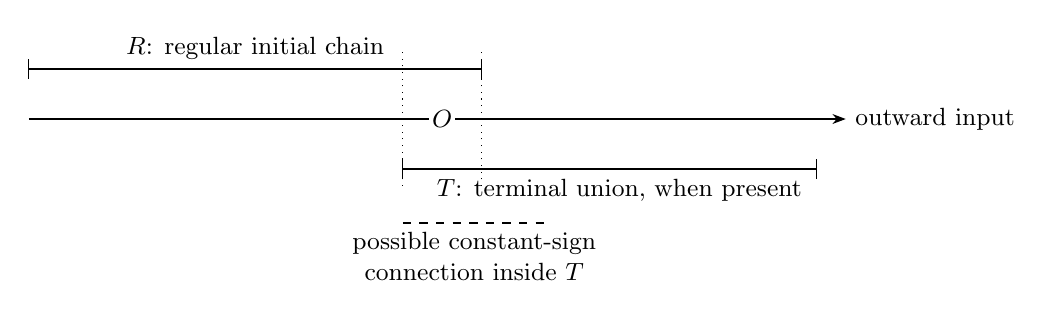
\begin{tikzpicture}[x=1.25cm,y=.85cm,>=Stealth,font=\small]
 \draw[->] (0,0)--(8.3,0) node[right] {outward input};
 \draw[thick] (0,.75)--(4.6,.75);
 \draw (0,.60)--(0,.90) (4.6,.60)--(4.6,.90);
 \node[above] at (2.3,.75) {$R$: regular initial chain};
 \draw[thick] (3.8,-.75)--(8,-.75);
 \draw (3.8,-.90)--(3.8,-.60) (8,-.90)--(8,-.60);
 \node[below] at (6,-.75) {$T$: terminal union, when present};
 \draw[dotted] (3.8,-1.0)--(3.8,1.05);
 \draw[dotted] (4.6,-1.0)--(4.6,1.05);
 \node[fill=white,inner sep=1pt] at (4.2,0) {$O$};
 \draw[thick,dashed] (3.8,-1.55)--(5.25,-1.55);
 \node[below,align=center] at (4.525,-1.55)
    {possible constant-sign\\connection inside $T$};
\end{tikzpicture}
\caption{Schematic intervals on one actual physical fibre with an outer
closing witness. $O$ is an open overlap. Near the parabolic corner $R$
includes the finite connection, wedge and regular secondary part.
The depicted terminal lower-loss connection, when present, remains
inside $T$. The lengths
carry no metric information, and the arrow orders inputs rather than
trajectories. Proposition~\ref{rw:ordered-cover} supplies these domains.}
\label{rw:physical:interval-scheme}
\end{figure}

We use the original and normalized generators
\[
 \tau_0=a+c,\quad \sigma_0=c(B+m),\qquad
 \tau_1=\bar a+\bar c,\quad
 \sigma_1=\bar c(\bar B+\bar m),
\]
so $\tau_0=\rho\tau_1$, $\sigma_0=\rho^3\sigma_1$,
$\epsilon=\rho^2$ and $\ell=\rho\nu$. Except when explicitly
discussing $\rho=0$, all normalized coordinates have $\rho>0$.
Reflect the whole field once, if necessary, to arrange $\ell\ge0$.
The new outgoing endpoint is the old incoming endpoint; reflection
does not preserve a previously selected numerical outgoing cutoff.
It preserves the original generator norms and cycle multiplicities
by Proposition~\ref{rw:geometry:reflection}.

\subsection{Cycle candidates, retained scales, and outer forcing}

Write
\[
 F_\pm(X)=1\pm\bar aX+\bar BX^2,\qquad
 \mathcal P=\{\bar c=\bar m=0,\ \bar B>0,\
           |\bar a|\le2\sqrt{\bar B}\}
\]
on the normalized max-norm face. At $\mathcal P$ one has
$\bar B\ge1/4$. Indeed either $\bar B=1$ or $|\bar a|=1$,
and the latter inequality gives $\bar B\ge1/4$.
The compactified interval $[0,\infty]$ is always given its ordinary
topology through $p\mapsto p/(1+p)$.
We first cover closing orbits, so that an outer orbit can supply a
coefficient inequality. We will extend the cover to the intervening
comparison arcs after proving that all of those arcs return.

\begin{lemma}[Refined candidate space]\label{rw:fibre:candidate-space}
The limiting data of parameter-dominant counted cycles have a compact
refinement with the following properties.
Away from $\mathcal P$ its coordinates are the normalized
coefficients and the two compactified actual endpoints.
Near $\mathcal P$ it additionally retains the secondary direction
$(C,M)$, the secondary scale and actual first-exit tags.
Every point has one of the local descriptions of Sections~7--10,
including their boundary faces. The same compactification can be
applied simultaneously to an outer cycle and any returning upper
arc between fixed positive initial endpoints and its endpoints.
The assertion about such additional arcs is compactness only;
their existence and local classification will be proved below.
\end{lemma}
\begin{proof}
Let $\chi>0$ be the fixed strong-entry constant in
Lemma~\ref{rw:finite:action-order}. For parameter-dominant
cycles, $p\ge\chi/2$, $q\ge\chi$. Take the intersection, as
$r\downarrow0$, of the closures of their data with $0<\rho<r$
in
\[
 \mathcal S\times[\chi/2,\infty]\times[\chi,\infty],
 \qquad
 \mathcal S=\{(\bar B,\bar m,\bar a,\bar c):
          \max(|\bar B|,|\bar m|,|\bar a|,|\bar c|)=1\}.
\]
This is a compact set. Its points satisfy the nonnegative lower
conditions of Lemma~\ref{rw:finite:lower-cones}. The parameter
$\nu$ tends to zero by Proposition~\ref{rw:geometry:flatness}.

Only the corner at $\mathcal P$ needs further coordinates. Put
\[
 \bar d=\bar c+\nu,\qquad
 \lambda=\max(|\bar d|,\sqrt{|\bar m|}),\qquad
 C=\bar d/\lambda,\quad M=\bar m/\lambda^2
 \quad(\lambda>0).
\]
The direction belongs to the compact face
$\mathcal D=\{\max(|C|,\sqrt{|M|})=1\}$. Use the fixed
sections of Lemma~\ref{rw:secondary:routing}. Retain a finite
flag specifying a wedge exit, a secondary exit, or their overlap.
For a wedge intersection retain $H\in[0,H_0]$ and, if
$H+\lambda>0$, the ratio
$\chi_{\rm exit}=H/(H+\lambda)$.
For a secondary intersection retain its actual radial coordinates
$R_{\rm in},R_{\rm out}\in[0,R_{\max}]$ on the sections
$\phi=\pm\lambda L$, together with
\[
 t=1/P,\qquad \widetilde t=1/Q,\qquad
 0\le t,\widetilde t\le1/p_* .
\]
Here $P,Q$ are the auxiliary linear-flow labels of
Lemma~\ref{rw:secondary:tags}, evaluated at those actual section
points; in particular $t=R/\bar x(T)$ on the incoming section.
They are not defined to be $\lambda p,\lambda q$.
Use a fixed placeholder for an inactive coordinate. Allow all the
indicated flags on an overlap, and take the closure of the resulting
actual-data graph in the finite union of these compact products,
also retaining $\lambda\in[0,\lambda_*]$.
Taking the closure retains radial limits without inverting a map
at zero radius. An orbit in an overlap may have two sets of tags;
keeping both copies preserves compactness and suffices for a finite
subcover.

If $H/\lambda$ tends
to infinity, routing is in the wedge and
$|\bar d|/H+|\bar m|/H^2$ tends to zero. For a finite ratio
the first-exit flag is retained: a first wedge exit has
$H/\lambda\ge L$ and hence the fixed wedge inequalities,
whereas a first secondary exit is in the secondary rectangle.
The equality face has the open overlap proved below. Radial escape is
$R=0$, equivalently $1/P=0$ or $1/Q=0$, and is retained in
the secondary infinity charts. The cases of a finite upper
threshold and its repeated limit are retained with their actual
deficits. Proposition~\ref{rw:secondary:exhaustion} classifies the
entire normalized face, including its repeated and weak boundaries,
and excludes another zero corner. For $\lambda=0$ an actual field
uses only the wedge; secondary directions there record limits with
$\lambda>0$. This classification applies to returning upper arcs.

For completeness the primary alternatives follow directly from
the upper linear flow. A finite nonregular pair is $(p_c,q_c)$
with $\bar m>0$. One finite and one infinite endpoint is a
strict real threshold, a repeated threshold with its whole interval
$p\ge P$, or the weak boundary $\bar m=0$; reflection gives
the other orientation. At two infinite endpoints the strict barrier
of Lemma~\ref{rw:finite:strict-barrier} gives
$\bar c^2+4\bar m\le0$. Strict focus, repeated upper root and
the cubic horizontal boundary are covered in Section~8; the joint
repeated center is Section~9. If $\bar m=0$, then $\bar c=0$
and the lower cones put the point in $\mathcal P$.
At a finite lower loss the first root, its double limit, or the
simultaneous pair gives the alternatives of Section~7.
The two-root and one-infinite statements include roots that escape
to infinity, so these faces are not omitted.

For an intermediate arc, take the product with a second set of actual
tags, sharing the coefficients but retaining its own section points
and first-exit flag.
Use independent initial bounds $p\ge p_0>0$, $q\ge q_0>0$ for
this copy; $q_0$ is uniform on the compact regular entrance.
Impose $p\le p^{\rm out}$, $q\le q^{\rm out}$ before
closing the actual-data graph. This remains a closed subset of a
compact product. The independent tags are needed because an
intermediate arc may take a wedge exit although the outer cycle takes
a secondary exit.
\end{proof}

\begin{lemma}[Uniform selection over compact fibres]
\label{rw:fibre:compact-selection}
In a compact metric product $X$ with continuous outer projection
$\pi:X\to B$ to a compact metric space, let
$X_r$ be the actual data with $0<\rho<r$ and put
$X_0=\bigcap_{r>0}\overline{X_r}$. If a finite union
$U$ of prepared open pieces contains the limiting fibre
$X_0\cap\pi^{-1}(\{b\})$, then
an outer neighborhood and a positive original scale cutoff can be
chosen so that every actual datum over that neighborhood belongs to
$U$. If this construction applies at every outer limit, finitely many
such choices give common cutoffs and bounds.
\end{lemma}
\begin{proof}
Choose $V$ with $\overline V$ disjoint from the compact set
$\pi(X_0\setminus U)$. If no scale cutoff worked, excluded actual data
over $V$ at scales tending to zero would have a subsequential limit in
$(X_0\setminus U)\cap\pi^{-1}(\overline V)$, a contradiction.
A finite outer subcover gives the common minimum scale cutoff and
maximum bounds. The same argument applies to the one-copy graph.
\end{proof}

\begin{lemma}[An endpoint cutoff chosen after contraction]
\label{rw:fibre:candidate-cover}
There is $p_\sharp>0$, chosen before the primary scale cutoff,
and finitely many local candidate neighborhoods that contain every
counted cycle with $p\ge p_\sharp/16$ at sufficiently small
original parameter. The regular member contains all sufficiently
small endpoint data with
$p_\sharp/16\le p\le p_\sharp/2$.
Each other member is either separated from its local center set
on its closure or has a common center-comparison domain and a
positive contraction exponent $b_j>p_\sharp^2$.
Secondary center estimates retain any prescribed finite power
of $\lambda$, or of the wedge height, before division.
\end{lemma}
\begin{proof}
Start with the nonregular part of the compact refined limit set
in Lemma~\ref{rw:fibre:candidate-space}. At a noncenter point
shrink the closed coefficient neighborhood away from the center
set. At a center point the classification gives a divided regular,
two-root, finite-saddle, weak, focus or joint chart.
There are no additional unprepared center losses: the exact
quasi-invariant \eqref{rw:finite:quasi-invariant} implies that an
incoming finite root on a center also has an outgoing root; a
one-infinite center has
$\bar a=-\bar c,\bar m=-\bar B$, so its finite lower factor
equals the upper entry factor; and a lower double root in the
secondary corner has $|\bar a|=2\sqrt{\bar B}>0$ and is off
the secondary center. The repeated coincidence is precisely the
joint chart.

On each center neighborhood, first retain a fixed lower subsegment
with positive action. After reducing the coefficient neighborhood,
normal contraction on this subsegment bounds the absolute coefficient
derivatives of the complete central deviations by
$C\epsilon^{-N}e^{-b_j/\epsilon}$, with $b_j>0$.
These are estimates of the absolute deviations; the logarithm of an
input-independent slow contraction may diverge. The large-power
preparation extends the same estimate by zero up to a lost exit.
Section~5 supplies the real center and the whole input domain on which
to divide. Double division uses two ordinary coefficient derivatives
of the absolute difference, and a single component uses one. The
budgets retained in Sections~7--9 include these derivatives; this step
takes no further input derivative.
In the corner use the weighted absolute estimates of
Lemma~\ref{rw:secondary:flat-budget}. For the present argument
retain power two before the coefficient division; if a later local
coordinate requires more, retain its specified finite power first.
The exact exponent in Proposition~\ref{rw:exact-long} makes
these choices uniform without bounding $\epsilon|\log\lambda|$.
For the wedge choose its fixed widths $|\gamma|,|J|<\delta$
inside the regular-lower center box whenever $|\bar a|$ is
small. The remaining wedge data have $|\bar a|$ bounded
below and are primary off-center data. Thus an off-center
secondary direction attached to a first wedge exit is not
used to estimate that exit by a power of $\lambda$; its
actual radial power is a power of $H$.

Take a finite cover of this refined nonregular set, and then choose
$p_\sharp\le\chi/2$ so that $p_\sharp^2<\min_j b_j$,
and decrease it to meet the small-endpoint error bounds in the
source and regular-column preparations. These choices precede
the smallness choice for $\epsilon$.
The compact complement of the chosen open neighborhoods is
strictly regular. Enlarge that compact regular set to contain
$p_\sharp/16\le p\le p_\sharp/2$ and the limits of cycles
in the two initial energy classes with $p\ge p_\sharp/16$.
The latter enlargement is regular: the source endpoints satisfy
$p=\sqrt{2\epsilon h e_+}\le2\sqrt\eta$ and
$q/p=\sqrt{e_-/e_+}=1+O(\eta)$, while the lower and upper
thresholds have a fixed positive lower bound. The compact-energy
class has $p,q\to0$ and causes no further endpoint limit.
The regular upper return and the positive lower polynomials
therefore give a common compact tube for this enlargement.

Apply Lemma~\ref{rw:fibre:compact-selection} to this one-copy
refined graph. Positive endpoint limits from the initial classes lie
in the regular enlargement, with $q$ bounded below when
$p\ge p_\sharp/16$ by the same source estimates. Thus the selected
finite family covers all the asserted cycle data.
\end{proof}

The candidate cover locates each outer closing orbit. To obtain one
sharp count, we next extract its coefficient inequality; saturation
then supplies all intervening comparison paths.

\begin{proposition}[Forcing supplied by an outer closing zero]
\label{rw:outer-forcing}
Choose the field orientation with $\ell\ge0$.
After a common original parameter shrink, a counted cycle with
$p\ge p_\sharp$ either lies in a constant-sign local comparison
whose full remaining physical passing interval is covered by that
same comparison, or supplies the coefficient inequality
\begin{equation}\label{rw:fibre:original-forcing}
 |\ell|\le e^{-p_\sharp^2/(20\epsilon)}
                    (|\tau_0|+|\sigma_0|).
\end{equation}
Equivalently,
\begin{equation}\label{rw:fibre:normalized-forcing}
 |\nu|\le e^{-p_\sharp^2/(20\epsilon)}
                    (|\tau_1|+\epsilon|\sigma_1|).
\end{equation}
An interior constant-sign piece is not sufficient for the first
alternative. On a center fibre with a closing zero there are no
isolated closing zeros.
\end{proposition}
\begin{proof}
Apply the candidate cover to the outer cycle. A constant-sign chart
containing the entire remaining passing interval gives the first
alternative. In every other chart we derive the coefficient inequality,
including on constant-sign pieces separated from the center set.

The nonnegative lower cone and
\eqref{rw:finite:action-budget}, applied at $p_\sharp$, give
\[
 s\le \exp[-p_\sharp^2/(5\epsilon)].
\]
Indeed
$A_+(p_\sharp)\ge
p_\sharp^2/[2(1+p_\sharp+p_\sharp^2)]$ and the error in
the budget is absorbed after $p_\sharp$ is fixed.
Since $|\ell|<3s$,
any closed primary neighborhood on which
$|\tau_1|+|\sigma_1|\ge g_0>0$ satisfies
\eqref{rw:fibre:original-forcing}: use
$|\tau_0|+|\sigma_0|\ge\rho^3g_0$ and absorb this fixed
power of $\rho$ in the strict gap between the two exponents.

At an off-center secondary first exit, the primary action estimate
alone does not retain the vanishing secondary weight. We use the exact
long match to recover it.
Suppose first $|C|\ge g_0/2$, where
$|\bar a|+|C|\ge g_0$ on the chosen closed neighborhood.
The exact long match gives an outgoing horizontal input
$u_+\le C_1\lambda^{k/b}$, with
$b=1-\epsilon\bar B$, $k=1-2\epsilon\bar B$.
The lower common power has exponent $b/(\epsilon\bar B)$.
The bounded scaled action and scaled prefactor, including a
possible additional contracting lower double passage, imply
\begin{equation}\label{rw:fibre:weighted-budget}
 s\le I_{\rm out}
       \le e^{C_0/\epsilon}\lambda^{k/(\epsilon\bar B)}.
\end{equation}
The first inequality uses the actual reference
$s_+=-\ell H_+\le0$. Choose $\kappa_*>0$ with
$k/\bar B\ge\kappa_*$, then $\lambda_0>0$ so that
\[
 (\kappa_*/2)\log(1/\lambda_0)
                    \ge C_0+p_\sharp^2/5,
 \qquad \epsilon\le\kappa_*/4.
\]
For $\lambda\le\lambda_0$,
\eqref{rw:fibre:weighted-budget} yields
$s\le\lambda^2e^{-p_\sharp^2/(5\epsilon)}$.
For $\lambda\ge\lambda_0$ the primary budget gives the same
bound with the fixed factor $\lambda_0^{-2}$. Consequently
$|\nu|\le\lambda|C|/2$ at small scale and
\[
 |\bar c|=|\lambda C-\nu|\ge\lambda g_0/4,\qquad
 |\sigma_0|\ge c\rho^3\lambda g_0 .
\]
The extra factor $\lambda^2$ proves
\eqref{rw:fibre:original-forcing} uniformly, even if
$\epsilon|\log\lambda|$ is arbitrarily large.
If $|C|<g_0/2$, then $|\bar a|\ge g_0/2$; the corner
has $|\bar c|<g_0/4$, so this reduces to the primary
off-center estimate.

On a retained center neighborhood, cancellation on the real center
recovers the generator factor. Write the complete closing function as
$Z-\rho\nu H$, with $H>h_*$ independent of the section input.
The actual center division gives
\[
 |Z|\le C\epsilon^{-N}e^{-b_j/\epsilon}
             (|\tau_1|+|\sigma_1|+|\nu|).
\]
The local inverse charts and the two ideal comparisons in
Proposition~\ref{rw:generator-division} justify the indicated
generators. In secondary variables retain the weighted version
before returning to primary coefficients: a term
$\lambda^2|C|$ is bounded by
$|\bar d|=\lambda|C|$, and the wedge version is identical
with $H^2|\gamma|\le|\bar d|$ and its retained height.
The small-$|\bar a|$ wedge box was included in these center
comparisons independently of its secondary direction. Since
$|\bar d|\le|\bar c|+|\nu|$ and
$\bar B+\bar m>1/8$ here, the resulting bound is again the
displayed primary one. No inverse power of $\lambda$ is
introduced.
At a closing zero Lemma~\ref{rw:centers:relative-forcing}
absorbs the $\nu$ term. Since $b_j>p_\sharp^2$, the fixed
powers of $\epsilon$ needed to return to original generators
are absorbed with room to spare.

Finally consider the compact regular member at $p\ge p_\sharp$.
Retain a slightly larger actual tube with $p\ge p_\sharp/2$.
The regular upper map has $q\ge p(1-p)$ at small endpoints;
hence both retained actions have a lower bound greater than
$p_\sharp^2/10$ after $p_\sharp$ is reduced. The regular
absolute maps and double center division yield
\[
 |\ell|\le C\epsilon^{-N}e^{-p_\sharp^2/(10\epsilon)}
                      (|\tau_0|+|\sigma_0|),
\]
which implies the required exponent $p_\sharp^2/20$.
The finite candidate cover makes these choices uniform. If the
generators vanish, absorption first gives $\nu=0$, and the actual
center identity excludes isolated zeros.
\end{proof}

\subsection{Equilibria and the three returning strips}

To continue the comparison paths between an initial input and an outer
cycle, we must exclude an equilibrium that could trap an intervening
orbit. We do this first, then fill the upper and two lower strips by
trajectories.

\begin{lemma}[Equilibria enclosed by counted cycles]
\label{rw:fibre:enclosed-equilibria}
On a common small original parameter neighborhood, the Jordan disk
of every counted cycle contains the origin and no other equilibrium.
The section points of any two counted cycles belong to one interval
of the actual return domain.
\end{lemma}
\begin{proof}
The origin has index one and remains the only equilibrium in a
fixed inner disk. The fixed regular collar strips remain free of
equilibria. Proposition~\ref{rw:collar} places every counted
cycle essentially in the collar, surrounding that disk. The upper
vertex calculation in that proposition leaves at most one additional
equilibrium in the upper chart, and it is a saddle.
It remains to exclude horizontal equilibria from the cycle's disk.

If $\rho=0$, then $B=m=a=c=0$ and $\dot x=-y$; the
equilibrium equations give only the origin. Suppose $\rho>0$.
In a horizontal chart $x=\sigma/r$, $y=v/r$, $\sigma=\pm1$,
the equation $\dot y=0$ is
\[
 \sigma(r+v)+dv^2+crv=0.
\]
Its unique small solution is $v=rh(r)$ with $h=-1+o(1)$.
Thus $|z|=|1+y|<\delta$ at any horizontal equilibrium.
The other equilibrium equation reads
\[
 1-z+\bar BX^2+\bar aX+\epsilon\bar m(1-z)^2=0.
\]
Choose fixed small $R,\delta>0$ and then small $\epsilon$.
The left side is positive for $|X|\le R$, $|z|\le\delta$,
so the equilibrium lies in one of the two half-strips $|X|>R$.

In the incoming half-strip put $T=1/(-X)$ and use the positive
time change $\dd\tau/\dd\xi=-X$. With
$\eta_\ell=\rho\ell$, the exact equations are
\begin{equation}\label{rw:fibre:horizontal-equilibrium-field}
\begin{split}
 T_\tau&=\epsilon T\bigl[\bar B-\bar aT+
        \{1-z+\epsilon\bar m(1-z)^2\}T^2\bigr],\\
 z_\tau&=-z+\epsilon\bar cTz(z-1)
                             +\eta_\ell T(1-z)^2 .
\end{split}
\end{equation}
On $0\le T\le1/R$, $|z|\le\delta$, the tangential derivatives
are $O(\epsilon)$ and the normal derivative is
$-1+O(\epsilon+|\eta_\ell|)$.
Extend to a slightly larger rectangle, preserving $T=0$ and
these strict margins. The normally contracting graph construction
used in Section~4 gives
\[
 z=g(T)=\eta_\ell T\,O_{C^2}(1),\qquad
 Z=z-g(T),\qquad Z_\tau=-\beta(T,Z)Z,\quad\beta>1/2.
\]
The two factors in $g$ follow by solving on $\eta_\ell=0$
and $T=0$, respectively, and dividing these vanishing factors
in the bounded graph family. Every equilibrium lies on $Z=0$.
The small original quantity is $\rho\ell$; no bound on
$\nu=\ell/\rho$ is used.

A counted cycle has $z>0$ by
Proposition~\ref{rw:geometry:cycle-height}. At $T=1/R$,
$0\le z\le\delta$, one has $T_\tau>0$, while
$|g|<\delta/2$. A cycle point with $Z<0$ cannot leave the
rectangle in backward time through $T=1/R$; it cannot reach
$z=\delta$ because $Z<0$ is preserved and $g<\delta/2$.
It cannot reach $z=0$, and its compact affine orbit stays away
from $T=0$. It would therefore remain in the rectangle for
all backward time, whereas $|Z|$ grows exponentially.
This is impossible. A periodic orbit on $Z=0$ would be a
nonconstant periodic orbit of the scalar equation on that graph,
also impossible. Every cycle point in this half-strip consequently
lies strictly above $g$.

An equilibrium with $0<z=g(T)<\delta$ is joined vertically to
$z=0$ without meeting the cycle: cycle points with that $T$
are above $g$, including any points above the rectangle.
The line $z=0$ is outside the cycle's disk, since the whole
cycle has $z>0$. Thus the equilibrium is outside the disk.
The same holds immediately if its height is nonpositive.
Reflecting the field and reversing time gives the argument on
the outgoing half-strip, for either sign of $\ell$.
The coordinate $T$ includes finite roots and roots escaping
to infinity, so no horizontal escape case remains.

The single upper saddle is now the only possible additional
equilibrium inside the disk. Its index would change the enclosed total
from one to zero, contradicting the index of a periodic orbit. Thus
only the origin is enclosed. Two counted cycles are nested essential
curves and bound an equilibrium-free annulus in the collar. Cut this
annulus at the transverse central section. The compact-limit argument
for the strips below shows that every intermediate section point
returns, placing both cycles in one interval of the actual return
domain.
\end{proof}

\begin{proposition}[Saturation of the physical interval]
\label{rw:saturation}
Assume \eqref{rw:fibre:original-forcing}, fix
$p_0\in[p_\sharp/8,p_\sharp/4]$, and let $\gamma$ be a counted
cycle with $p_\gamma>p_0$. Every input
$p\in[p_0,p_\gamma]$ has an actual upper return $q(p)$
and both actual lower central intersections. They satisfy
\[
 q'(p)>0,\qquad L_+'(p)<0,\qquad L_-'(q)<0,
 \qquad
 L_+(p),\ L_-(q(p))\ge s_\gamma>0.
\]
All three arcs, and the segment joining their central endpoints,
lie in the fixed collar. This statement holds at nonclosing inputs
as well as on periodic orbits.
\end{proposition}
\begin{proof}
At $p_0$ the fixed small-endpoint upper map and both regular
lower maps exist. After reducing $p_\sharp$, their two actions
are at most $p_\sharp^2/31$ uniformly in the stated interval
for $p_0$. Their positive homogeneous amplitudes are bounded
below by a fixed positive prefactor times
$e^{-p_\sharp^2/(31\epsilon)}$.
The actual signed reference contributions are $O(|\ell|)$.
Since the original generator norm is bounded and the forcing
exponent is $p_\sharp^2/20$, both complete central heights are
positive for sufficiently small scale. Their arcs lie in the collar
by the regular construction.

The axis endpoints of the three initial arcs lie inside the
corresponding endpoints of $\gamma$. Since trajectories cannot cross
$\gamma$, the arcs stay in its disk. Join their central endpoints by
the central crosscut. Each lower path stays in its own half-plane until
its first central intersection, so it meets the crosscut only there.
The three arcs and the crosscut form a simple essential curve in the
collar, inside $\gamma$, whether or not its two central values coincide.

The initial and outer upper arcs, joined by the two axis segments,
bound a compact equilibrium-free strip by
Lemma~\ref{rw:fibre:enclosed-equilibria}. Since $\dot y=x$ on
$y=0$, the positive axis segment is an entrance, the negative one
an exit, and the orbit sides cannot be crossed. A nonexiting orbit
would have an equilibrium-free compact $\omega$-limit set, hence a
periodic orbit by Poincar\'e--Bendixson. Its Jordan disk lies in
$y>0$ inside $\gamma$ and contains no equilibrium, contradicting
the periodic-orbit index. Thus every intermediate upper entry returns, with
$q_0\le q(p)\le q_\gamma$. The transverse flow determinant
has a fixed sign and gives $q'(p)>0$.

Construct the right and left lower strips from the corresponding
initial and outer arcs, an axis segment, and a central crosscut.
They are equilibrium-free as well. On the right use backward
time, so the positive axis segment is an entrance; on the left
use forward time and the negative axis segment is an entrance.
The central crosscuts are exits because $\dot x>3/4$ on the
fixed central rectangle. The same compact-limit and index argument
gives both central intersections at every intermediate endpoint.
Transversality and endpoint order give $L_+'(p)<0$, $L_-'(q)<0$;
their minimum heights occur on $\gamma$ and equal $s_\gamma>0$.

The three strips and the joining central segments lie in the annulus
between the two essential curves, hence remain in the fixed collar.
The nonexit contradiction uses compactness for each fixed field;
flight times may diverge as a saddle or slow gap tends to zero.
\end{proof}

On this physical interval keep the actual central height as output.
The fixed weak references give
\[
 F(p)=L_+(p)-L_-(q(p))=U(p)-V(p)-\rho\nu H,\qquad H>0,
\]
where $H$ is independent of $p$ and $U',V'<0$. Consequently
\begin{equation}\label{rw:fibre:physical-log}
 K=\epsilon\log(V'/U'),\qquad
 F'=U'(1-e^{K/\epsilon}).
\end{equation}
A common regular input change and a change of the fixed additive
references preserve $K$ on this orbit interval. We keep the original
central height as output, since a nonlinear output change need not
preserve it. The signed center-comparison domains used to estimate
these functions are auxiliary; the physical interval of
Proposition~\ref{rw:saturation} has positive complete central heights.

\subsection{The ordered cover of all intermediate arcs}

Saturation supplies the intermediate paths. We must now order their
local descriptions so that separate endpoint bounds become a bound
on one interval. The whole-passage tests will give a regular prefix
followed by at most one terminal union. At the parabolic corner this
requires two connections: from the finite family to the wedge, and
from the wedge to the secondary family.

\begin{lemma}[The two parabolic connections]
\label{rw:fibre:parabolic-connections}
Near $\mathcal P$ the finite regular family connects by an actual
open overlap to the wedge, possibly through a constant-sign lower
loss interval. The wedge in turn has an actual open overlap with
the regular secondary family. The construction applies to the
nonperiodic returning arcs in Proposition~\ref{rw:saturation}.
\end{lemma}
\begin{proof}
Consider first the incoming lower double boundary
$\bar a_*=2\sqrt{\bar B_*}$ and put
$r=1/\sqrt{\bar B_*}$. The limiting upper return has $q=p$.
For $0<p<r$,
\[
 A_-(p)-A_+(p)
 =2\bar a_*\int_0^p
               \frac{X^2}{F_+(X)F_-(X)}\,\dd X>0.
\]
Thus $K<0$ on every fixed compact regular initial interval,
uniformly in a smaller off-center neighborhood.
Let $C_w=\sqrt{1+2w_0}/w_0$. The limiting upper parabola
$Y=(p^2-X^2)/2$ meets $w=w_0$ at $H=C_w/p$.
Choose $L_1>2r$ so large that $C_w/L_1<H_0/2$.
The upper arcs for $L_1\le p\le2L_1$ form a compact regular
family; their transverse intersections persist and belong to
the wedge after the coefficients are reduced.

The incoming action tends to infinity as its first double root
is approached from below. Choose $R<r$ with
\[
 A_-(R)>\max_{p\le2L_1}A_+(p)+3,
\]
where the maximum is on the retained regular outgoing interval.
Then choose a fixed $p_1<r$ with $p_1>R+2\zeta$ for some
$\zeta>0$. Uniform convergence of the regular upper map to
$q=p$ on $[p_1,2L_1]$ gives $q(p)>R+\zeta$ there.
Lemma~\ref{rw:finite:incoming-contraction} now gives $K<0$
on its entire physical passing part, even beyond the lower
root where the ordinary regular action formula no longer applies.
This interval overlaps both the regular initial family and the
wedge. The corresponding lower slow action in the wedge has
the same strict sign and dominates its bounded remainder.
Reflection gives the other lower double boundary and reverses
the sign. Away from these boundary neighborhoods the lower
factors have a common positive margin on every retained finite
interval, so the regular family connects directly to the wedge.

For the wedge--secondary overlap, choose the fixed $L$ in secondary
routing large enough before decreasing any scale. Require
$2/L<\delta$ and $4/L^2<\delta$. At
$w=w_0$, $H=k_0\lambda L$, with $1/2<k_0<1$, the exact
secondary coordinates are
\[
 \widehat x=\frac1{k_0Lw_0},\qquad
 \widehat z=\frac1{k_0^2L^2w_0}.
\]
The auxiliary linear flow defining the actual tags gives
$P,Q=O(C_w/L)$ uniformly for bounded $(C,M)$.
At $C=M=0$ the values are $C_w/(k_0L)$; the perturbation
on these short arcs is of higher order in $1/L$.
Increase $L$ so all these tags lie in one compact regular
interval below the finite secondary thresholds.
The wedge inequalities are strict, and the same actual arcs
meet the secondary sections before reaching $w=w_0$.
Transversality persists as $k_0$ varies on a smaller open subinterval
of $(1/2,1)$. Thus an open family of the same returning arcs has both
descriptions, including the nonclosing comparisons.
\end{proof}

\begin{proposition}[An ordered cover on each physical fibre]
\label{rw:ordered-cover}
After a common original parameter shrink, every physical interval
of Proposition~\ref{rw:saturation} is covered by a connected
regular initial part and an ordered union of the local passing
charts of Sections~7--10. Their adjacent members overlap on
actual orbits. At a joint repeated center one contact member and
the full separated member form a single union. Near $\mathcal P$
the initial part includes the finite connection, the wedge and
the regular secondary part.
After grouping overlapping descriptions of the same end, there
is at most one terminal union after this initial part.
It may contain a constant-sign lower-loss connection followed
by a singular upper end; that connection is retained as its
own piece.

The coefficient neighborhoods and all cutoffs can be selected
from a finite family, independently of the chosen outer cycle.
The order includes signed split-root faces and the repeated
one-infinite interval. Each local derivative estimate is applied
on its stated whole-passage domain. This proposition makes no
sum of local zero bounds.
\end{proposition}
\begin{proof}
Fix the finite derivative orders of Sections~7--10 and retain their
larger construction domains before reducing sections or coefficient
neighborhoods. Saturation supplies actual upper and lower returns
with positive central heights on $[p_0,p_\gamma]$.
Since $q'>0$, their endpoints satisfy $p\le p_\gamma$,
$q\le q_\gamma$ and inherit the outer lower cones.

The key ordering fact is that a lost passing component cannot reappear.
The exact lower factor on the fixed phase interval is
\[
 F_I(x)=\bar B-\bar ax+(1+\epsilon\bar m)x^2
 -\epsilon\nu(1+2\epsilon\bar m)x^3H(x)
 +\epsilon^3\nu^2\bar m x^4H(x)^2.
\]
By Proposition~\ref{rw:phase}, it is strictly convex and positive
near the fixed exit $x_R$. Lemma~\ref{rw:transitions:lower-sections}
requires $F_I(s)>0$ at every point between the actual entry and
$x_R$. Thus only the component adjoining $x_R$ passes: if a root
is present, the entry must lie to the right of its last root.
The entry decreases as its actual endpoint increases, since
$T=1/p$ or $1/q$ and $t_T>0$. Its allowed endpoints consequently
form one outward initial interval. Entry positivity in the other
component would not suffice. Also $F_I'(0)=-\bar a$ and its
reflected derivative is $\bar a$; strict convexity permits an
interior positive double minimum on at most one of the two sides.

The primary upper slow tests have the same one-sided form. For a repeated
factor $v^2+\mu_U$, passage to the positive fixed exit requires
$\mu_U>0$ or $v>\sqrt{-\mu_U}$; its actual finite entry decreases
with $p$. This retains the negative entries beyond the repeated
threshold whenever they pass. For the weak factor $u(\gamma+u)$,
the whole domain is $\max(0,-\gamma)<u<u_0$, and
$p=\hat p-t(u)$ with $t'>0$. At joint contact both calibrated
entries decrease, so the two whole-path tests are intersections
of one-sided restrictions. General horizontal factors use the
whole lower test above; a smaller monotone block alone permits
an endpoint test. Signed auxiliary coefficient comparisons do not
remove physical inputs, whose complete central heights are positive
by saturation.

The increasing upper graph and its reflected inverse are those of
Lemma~\ref{rw:finite:upper-return}. Its nonregular ends are classified
in Lemma~\ref{rw:fibre:candidate-space}, with the full repeated
interval $p\ge P$, $q=\infty$ retained. Following the graph outward
gives these terminal templates:
\begin{itemize}
\item At a regular finite upper end, the first lower loss is a
single root or the simultaneous simple-root pair. A simple root
terminates passage; a double retains its signed slow alternatives.
\item At a finite upper saddle, the lower paths are regular, in
one or both contact neighborhoods, or have one incoming double-loss
connection before the saddle. An outgoing double with regular
incoming outer data is excluded by
Lemma~\ref{rw:finite:action-order}, applied to the outer cycle.
The incoming connection is the whole constant-sign interval of
Lemma~\ref{rw:finite:incoming-contraction}.
\item At a one-infinite end, a lower root can precede, coincide
with, or follow the upper threshold. These give respectively the
lower connection, the contact neighborhood, or the upper-tail piece
followed by the lower loss. A root escaping to infinity retains
its finite-root and cubic descriptions in the same family.
\item At two infinite endpoints the lower cones exclude a prior
simple root. Section~8 supplies the strict-focus, one lower-double,
repeated, opposing-slow and cubic alternatives; Section~9 supplies
the joint contact interval and its full separated tail.
\end{itemize}
A finite saddle has one returning quadrant, while the strict,
repeated and weak preparations have the through components just
described. Together with the monotone entry tests, this excludes a
second independent upper end or a return after a split-root
obstruction. The pieces of each listed end therefore form one
terminal union, retaining a preceding constant-sign lower connection
as a separate piece within it.

Near $\mathcal P$, use the actual first exits and tags of
Proposition~\ref{rw:secondary:exhaustion}. Routing confines a
returning arc to the fixed secondary rectangle and uniqueness
excludes another middle excursion. The normalized face
$\max(|C|,\sqrt{|M|})=1$ has the finite-saddle, strict real,
repeated, weak and focus alternatives, including $1/P=0$ and
$1/Q=0$. The repeated row retains its full label interval.
At its weak end the actual tag is $P=P_s-\psi(t(u))$ with
$\psi'>c$; again outward motion decreases $u$.
The preceding lemma inserts the finite connection, wedge and
regular secondary prefix. The same first-threshold reasoning then
gives one secondary terminal family; a lower-double overlay can
add its retained connection but cannot add an opposing double or
another returning quadrant.

Retain actual open seams before reducing the scale: a fixed positive
deficit crosscut between finite regular and singular pieces; the
joint contact/separated overlap $P+d<p<P+2d$ with both gaps
positive; and a fixed reciprocal annulus before either slow block,
using Lemma~\ref{rw:transitions:common-input}. These connectors
are transverse with bounded inverses. The finite lower-double
bridge has the strict action margin of the preceding lemma.
That lemma also supplies the finite--wedge and wedge--secondary
transverse overlaps. Within the secondary family retain its fixed
deficit crosscuts and reciprocal annuli. Adjacent strict, repeated
and weak faces use their own uniform preparations; no estimate at
a fixed positive eigenvalue ratio is extended across zero or infinity.
All seams compare the same original central function.

Apply Lemma~\ref{rw:fibre:compact-selection} to the joint compactification
of Lemma~\ref{rw:fibre:candidate-space}: the intermediate copy has
independent bounds $p\ge p_0$, $q\ge q_0>0$, its own first-exit tags,
and $p\le p^{\rm out}$, $q\le q^{\rm out}$. Each compact limiting
fibre is covered by the ordered pieces and their whole regular prefix.
The retained crosscuts, action margins and transverse seams make this
an open cover, including reciprocal radial ends; the one-sided entry
tests preserve order. Positive endpoint limits from the initial energy
classes use the regular enlargement in
Lemma~\ref{rw:fibre:candidate-cover}. Thus the lemma gives common
cutoffs after all sections, derivative budgets and overlap margins
have been fixed.
\end{proof}

\subsection{Transport in the original coefficient fibre}

We transfer the outer orbit's inequality to the splitting, gap and
saddle-ratio coordinates. The comparisons below may contain $|\nu|$;
the exponential factor absorbs it on the fixed coefficient fibre.

\begin{proposition}[Uniform coefficient and domain transport]
\label{rw:coefficient-transport}
On the ordered cover of Proposition~\ref{rw:ordered-cover},
the fixed original inequality
\eqref{rw:fibre:original-forcing} supplies the relative coefficient
bounds used in the local critical-function estimates, uniformly at
all physical inputs, including
nonclosing inputs. More precisely, for each local center-generator
size $I_{\rm loc}$ used in Sections~7--10 there is a modulus
$\eta_{\rm loc}(\epsilon)\to0$ such that
\[
 |\nu|\le\eta_{\rm loc}(\epsilon)I_{\rm loc}.
\]
The coefficient constants and moduli are common to the finite cover.
The coefficient divisions take place on the larger comparison
domains of Section~5 and the corresponding secondary domains.
The counted inputs remain on the positive-central physical interval.
If a local generator size vanishes, absorption first gives
$\nu=0$ and then the relevant exact center identity.
\end{proposition}
\begin{proof}
Set $\delta_\epsilon=e^{-p_\sharp^2/(20\epsilon)}$.
The original inequality is
\begin{equation}\label{rw:fibre:transport-start}
 |\nu|\le\delta_\epsilon
                 (|\tau_1|+\epsilon|\sigma_1|)
          \le\delta_\epsilon
                 (|\tau_1|+|\sigma_1|).
\end{equation}
We compare the original generators with the local transverse
coefficients in each type of chart.

On regular and strict-focus charts take
$I_{\rm loc}=|\tau_1|+|\sigma_1|$. At a two-lower-root match,
the strict splitting derivative of
Proposition~\ref{rw:finite:two-root-count} makes
$(\bar a,\delta,\nu)$ a bounded inverse chart on a larger box.
Here $\delta$ is the actual strong-intersection splitting.
Single division from its exact reversible axis gives
\[
 |\tau_1|+|\sigma_1|
                 \le C(|\bar a|+|\delta|+|\nu|).
\]
The finite upper saddle uses $(\bar a,\kappa,\nu)$ with the
actual $\kappa=r-1=-\operatorname{tr}/\lambda_+$; the derivative
$\partial_{\bar c}\kappa=-1/\sqrt{\bar m}+O(\epsilon)$ has a
nonzero margin. The same division, already described after
Proposition~\ref{rw:generator-division}, gives
$|\tau_1|+|\sigma_1|\le C(|\bar a|+|\kappa|+|\nu|)$.
Off these center axes the transverse size has a positive lower
bound on each smaller closed chart.

At the finite three-saddle intersection,
\eqref{rw:centers:ideal-comparison} gives
\[
 |\tau_1|+|\sigma_1|+|\nu|
            \asymp |\xi_2|+|\kappa\xi_1|+|\nu|.
\]
Thus take $I_{\rm loc}=|\xi_2|+|\kappa\xi_1|$; the product
retains both intersecting center branches. The double-division
segments and derivative budget are those of Section~5.

At a strict one-infinite simple-root coincidence use the exact
splitting $\delta$ and the actual scaled exponent difference
$g$. On its strict compact row the determinant of this coordinate
change tends to
\[
 \frac{p_c^4}{\bar B(1-\bar Bp_c^2)^3}>0,
\]
up to the positive unit from the regular power coordinate.
The calculation and the equality of the actual leading powers
on the second center are in
Proposition~\ref{rw:infinity:strict-lower-loss}.
Their bounded inverse and single division give
$|\tau_1|+|\sigma_1|\le C(|\delta|+|g|+|\nu|)$.
At the repeated and weak faces use instead the two comparisons
\eqref{rw:centers:single-ideal-comparison}, with local sizes
$|\tau|+|\zeta|$ and $|d_s|+|\varsigma|$, respectively.
Their inverse charts and exact center axes were proved in
Proposition~\ref{rw:center-coordinates}; the repeated comparison
uses \eqref{rw:coordinates:zeta-identity}, rather than the strict-row
determinant. The fixed-mean and lifted-contact comparisons, and the
single weak offset $\bar B+K_*A$ of
Proposition~\ref{rw:domains:weak}, are defined on larger domains
containing every original input and the whole coefficient segments.
At a cubic two-infinite end $\bar B=0,\bar m<0$,
$|\bar B+\bar m|$ has a positive margin. Hence
$|\tau_1|+|\sigma_1|\asymp|\bar a|+|\bar c|$,
the cubic generator size. On other constant-sign pieces
either the same bounded comparison applies or the
transverse size is bounded below; no division at a vanishing
gap is needed.

At the parabolic corner we must retain the scale weights before
comparing generator sizes. Since
$\bar B+\bar m>1/8$, bounded normalized coefficients give
\[
 |\tau_1|+|\sigma_1|
       \le C(|\bar a|+|\bar c|)
       \le C(|\bar a|+|\bar d|+|\nu|).
\]
Inserting this in \eqref{rw:fibre:transport-start} and
absorbing gives
\begin{equation}\label{rw:fibre:weighted-transport}
 |\nu|\le2C\delta_\epsilon(|\bar a|+|\bar d|).
\end{equation}
On the wedge, $\bar d=H\gamma$ with $H\le H_0<1$;
on the secondary charts, $\bar d=\lambda C$ with
$\lambda\le\lambda_*<1$. It follows, uniformly at every
actual input, that the forcing is small relative to the local
sizes $|\bar a|+|\gamma|$ and $|\bar a|+|C|$.
The stronger weighted inequality
\eqref{rw:fibre:weighted-transport} is retained whenever
those local expressions are returned to original coefficients.
The wedge bound in \eqref{rw:secondary:critical-forcing} retains
$|\bar a|+|\bar d|$; the secondary bound uses $|\bar a|+|C|$.
The additional powers in \eqref{rw:secondary:local-forcing} arise
when an actual secondary closing witness supplies its absolute
budget; they are stronger than the bounds used here.

Near a finite secondary upper saddle the exact ratio calculation
\eqref{rw:secondary:saddle-ratio} has a nonzero derivative
in $C$ and yields
\[
 |C|\le C_0\bigl(|\kappa|+
                  \epsilon\lambda|\bar a|
                  +\epsilon\lambda|\nu|\bigr).
\]
Thus the preceding bound implies
$|\nu|\le\widetilde\eta(\epsilon)
 (|\bar a|+|\kappa|)$ after one further absorption.
The estimate therefore uses the actual ratio of the secondary field,
including its coefficient error relative to the limiting linear field.
On the weak and real repeated secondary rows $|C|$ has a
positive margin on the normalized face, so their transverse
size is bounded below. They need no inverse coordinate
division at the vanishing weak eigenvalue. A strict focus
center has its regular division in $(\bar a,C)$, and the
finite saddle center was treated above. These neighborhoods
cover the normalized face with the adjacent strict rows,
so the constants are uniform on their common boundary faces.

In every unweighted comparison we have obtained
$I_{\rm global}\le C(I_{\rm loc}+|\nu|)$.
Choose the common scale with $C\delta_\epsilon<1/2$;
then \eqref{rw:fibre:transport-start} gives
$|\nu|\le2C\delta_\epsilon I_{\rm loc}$.
The weighted comparisons have just given the same conclusion
with their explicitly retained factors. If $I_{\rm loc}=0$,
this inequality gives $\nu=0$ before any division by that
size. The inverse coordinate identity then places the field
on its real center axis, so its actual compared maps agree.
This deals with the zero-size case as well.

These are coefficient inequalities, so they hold also at nonclosing
inputs. All divisions use the larger domains of Section~5, while
saturation supplies positive central heights for the original field.
Taking the largest of the finite coefficient bounds makes the
absorptions and moduli uniform on the whole interval.
\end{proof}


\section{Entrance counts and the uniform upper bound}
\label{rw:upper-section}

The physical interval of Section~11 carries one original-height
derivative logarithm $K$. Its regular pieces have at most one crossing.
The three-saddle and weak endpoint estimates alone allow four closing
zeros, so they cannot give the sharp bound. The terminal arguments
below use the sign left by the regular part to bound $K$ by two zeros
on the whole interval. If a small cycle supplies the stronger entrance
sign, the regular part is zero-free and the bound improves to one.
These are the two counts required by Section~\ref{rw:counting}, in the
fixed-field orientation of Section~2.

We first derive the entrance from a small cycle and carry it along
the regular chain. The primary and secondary terminal arguments then
give the whole-interval count and the uniform upper bound.

\subsection{What a small cycle supplies at the common entrance}

Use the fixed-field orientation $\ell\ge0$ of
Section~\ref{rw:geometry}, with the reflection-symmetric thresholds
of Section~\ref{rw:counting}. The coefficient divisions are those
of the original signed auxiliary maps.
The source representative counts the small cycles and determines the
ratio of the two homogeneous generators. To obtain the entrance sign
of $K$, we then evaluate the regular comparison in the original central
height. This change of representation is necessary because a unit
relating closing functions need not preserve their derivative zeros.

\begin{proposition}\label{rw:small-entrance}
After a common neighborhood restriction, suppose $\rho>0$ and
\eqref{rw:counting:forcing} holds. There is at most one counted
cycle with $p<p_\sharp/4$, and it is simple. A counted cycle with
$p<p_\sharp/8$ implies
\begin{equation}\label{rw:upper:small-ratio}
 \tau_1\sigma_1<0,\qquad
 0<-\tau_1/\sigma_1\le p_\sharp^2/300.
\end{equation}
The actual regular comparison at $p_0=p_\sharp/4$ then satisfies
$\operatorname{sign}K(p_0)=-\operatorname{sign}\sigma_1$.
Thus it supplies the precise signed entrance of hypothesis
\textup{(III)} in Section~\ref{rw:counting}.
\end{proposition}
\begin{proof}
The endpoint action bound of Section~\ref{rw:finite:geometry},
with the fixed primary normalization, places every parameter-dominant
cycle beyond $p>\eta/8\ge p_\sharp$; the same bound is recorded
in the physical cover of Section~11. Hence the small cycles here
belong to the two initial energy classes, and are zeros of the one
function constructed in Proposition~\ref{rw:initial-joint-bound}.
In the source class its outgoing action satisfies
\[
 p^2=2e_+\epsilon h,\qquad |e_+-1|<1/1024.
\]
For a cycle with $p<p_\sharp/4$ this gives
$\epsilon h<p_\sharp^2/31$. On the compact energy class the
same inequality follows from $h\le H_*$ after the scale cutoff
is reduced. Let $J_0$ be the initial-energy interval up to that
upper bound; it contains all these cycles, with their multiplicities.
Its lower energy bound is the fixed $h(z_L)>H_{\rm ECT}+2$.
We do not use any ECT assertion near energy zero.

Write the actual source representative as
\[
 F_{\rm src}=\tau_0 f_1+\sigma_0 f_2+f_3,
 \qquad Q=f_2/f_1,\quad g=f_3/f_1.
\]
The compact overlap and the source derivative estimates in Section~6
give on this single initial-energy interval
\[
 Q\ge q_*>0,\qquad Q'\ge q_0>0,\qquad Q\le C_Qh.
\]
On the compact interval these inequalities follow from the first two
ordered Wronskians and fixed coefficient convergence; on the source
tail they follow from $Q=hC/A$, $Q_h>1/5$. The fixed overlap joins
the same two columns, so their signs can be tested on the union.

On $J_0$ we need the line-breaking contribution and its ordinary
energy derivative to be exponentially smaller than the homogeneous
coefficient norm. The signed compact contribution is $\ell$ times a
bounded coefficient. On the source part it is the exact logarithmic
forcing divided by $h^{3/2}A$.
Since $\widehat\ell=\ell/s$ and $s^{-1}=e^{h+1-s}\le e^{h+1}$,
\eqref{rw:counting:forcing} and the source logarithmic estimates
yield
\begin{equation}\label{rw:upper:small-forcing}
 |g|+|g'|\le C\exp\left(1-\frac{11p_\sharp^2}{620\epsilon}\right)
                      (|\tau_0|+|\sigma_0|)
       =:\vartheta_0(|\tau_0|+|\sigma_0|).
\end{equation}
Here $1/20-1/31=11/620$. The same bound applies to the fixed cutoff
terms on the compact overlap. The source logarithms are evaluated at
$\widehat\ell=o(1)$ on this smaller interval, so their denominators
have fixed margins. The derivative is the actual fixed-coefficient
energy derivative, not an independent source derivative.

If both homogeneous generators vanish, forcing gives $\ell=0$,
and the center identity contributes no isolated zero. Otherwise
\[
 F_{\rm src}/f_1=\tau_0+\sigma_0Q+g,
 \qquad (F_{\rm src}/f_1)'=\sigma_0Q'+g'.
\]
If $|\sigma_0|q_0>\vartheta_0(|\tau_0|+|\sigma_0|)$,
this derivative has a strict sign on all of $J_0$. Every zero is
therefore simple and there is at most one. In the complementary
case $|\sigma_0|\le2\vartheta_0|\tau_0|/q_0$ at small scale,
and
\[
 |F_{\rm src}/f_1|\ge |\tau_0|
 \left(1-\frac{2\vartheta_0 C_Qp_\sharp^2}{31q_0\epsilon}
                         -2\vartheta_0\right)>0.
\]
The exponential absorbs $\epsilon^{-1}$, so there is no zero.
This proves uniqueness and simplicity on the whole small-cycle set.

At the smaller cycle, with energy $h_y$, the same equation gives
\[
 -\frac{\tau_0}{\sigma_0}
 =Q(h_y)+g(h_y)/\sigma_0,
 \qquad |g/\sigma_0|\le\vartheta_0(1+|\tau_0/\sigma_0|).
\]
For small $\vartheta_0$, absorb the ratio on the right. The positive
lower bound $Q\ge q_*$ proves the strict negative sign of
$\tau_0/\sigma_0$. Moreover $\epsilon h_y<p_\sharp^2/127$.
The independent source constants give $C/A\to2/5$. Choose a fixed
$H_1\ge H_*+1$ so that its scale-tail error is below $1/100$,
then choose $p_\sharp$ small so that the coefficient error on this
energy range is below $1/100$. For $h\ge H_1$, $Q\le0.42h$;
below it $Q\le C_QH_1$. Therefore
\[
 \epsilon Q(h_y)\le
 \max(0.42p_\sharp^2/127,\epsilon C_QH_1)
                    \le p_\sharp^2/302
\]
after reducing the primary scale. The strict inequality
$0.42/127<1/302$ and the exponential error leave the margin to
$1/300$. Since $\tau_1/\sigma_1=\epsilon\tau_0/\sigma_0$,
this proves \eqref{rw:upper:small-ratio}.

The generator ratio now determines the entrance sign of the original
central comparison.
The physical-fibre construction in Section~11 includes the regular
point $p_0=p_\sharp/4$. The two regular columns in
Lemma~\ref{rw:regular-columns} satisfy
$C/A=p^2/5+O(p^3)$, uniformly on the normalized compact coefficient
set. Thus at this fixed point $C/A\ge p_\sharp^2/85$ after
choosing $p_\sharp$ small. Let
$w=(\tau_1,\sigma_1)/(|\tau_1|+|\sigma_1|)$.
Equation \eqref{rw:upper:small-ratio} makes
$w_1+w_2C/A$ have sign $\sigma_1$ and modulus at least
$p_\sharp^2/200$. The exact regular representation, divided by
this generator norm, is
\[
 K(p_0)/(|\tau_1|+|\sigma_1|)
          =-A(p_0)(w_1+w_2C(p_0)/A(p_0))+e(p_0).
\]
The positive $A(p_0)$ has a fixed margin, and regular coefficient
convergence together with the fixed-field forcing makes $e(p_0)$
smaller than half the preceding margin. Consequently $K(p_0)$ has
sign $-\sigma_1$, as required. All choices preceded the fixed field
and its cycle. Reflection transfers this statement with its actual
outgoing label and the identity \eqref{rw:counting:reflection}.
\end{proof}

\subsection{The complete regular chain}

The regular primary, wedge and secondary comparisons form one chain.
A common crossing direction on their actual overlaps gives a single
zero bound for $K$. Near the parabolic corner, the primary coefficient
cone shows that the outward direction is $-\operatorname{sign}C$,
with $C=\bar d/\lambda$.

\begin{proposition}\label{rw:regular-chain}
Assume the fixed-field inequality \eqref{rw:counting:forcing}.
The regular initial part of the ordered physical interval has at
most one zero of $K$, and that zero is simple. Near $\mathcal P$
this assertion includes the finite connection, the wedge and the
regular secondary tags, with their actual overlaps.

If a primary regular zero has occurred, its subsequent sign and
outward derivative have sign $-\sigma_1$ on the remaining
regular chain. The same conclusion holds if its initial point
has
\begin{equation}\label{rw:merge:strong-entry}
 \tau_1\sigma_1<0,\qquad
 \operatorname{sign}K=-\operatorname{sign}\sigma_1;
\end{equation}
in that case the regular chain is zero-free.
If the first zero instead occurs in the wedge or in the regular
secondary part, its subsequent sign and outward derivative have
sign $-\bar d$, and $\bar a\bar d<0$.
In particular a secondary terminal after that zero receives
$\bar aC<0$ and $K$ of sign $-C$.
\end{proposition}
\begin{proof}
Saturation and coefficient transport give the positive-central
interval with fixed-fibre forcing. The common-input identity
\eqref{rw:counting:input-change} identifies $K$ on its overlaps.

On the primary compact regular part
Lemma~\ref{rw:finite:regular-direction} gives at most one
simple zero and its outward direction $-\sigma_1$.
At a zero, or under \eqref{rw:merge:strong-entry}, the
positive column quotient on a fixed regular overlap gives
\begin{equation}\label{rw:merge:primary-cone}
 |\tau_1|\le C|\sigma_1|,\qquad
 |\nu|\le C e^{-p_\sharp^2/(20\epsilon)}|\sigma_1|.
\end{equation}
The second inequality involves coefficients only, so it persists
as the input moves along the chain.
Near $\mathcal P$, $\bar B+\bar m$ has a fixed positive
margin. Thus $\bar c$ has the sign of $\sigma_1$,
$|\bar a|\le C|\bar c|$, and
$\bar a\bar c<0$: the latter follows from
$(\bar a+\bar c)\bar c<0$.
Equation \eqref{rw:merge:primary-cone} makes
$\nu=o(|\bar c|)$, so $\bar d=\bar c+\nu$ has that same
sign and $\bar a\bar d<0$.
For $\lambda>0$, $C=\bar d/\lambda$ has that sign too.
No division of the error estimate by $\lambda$ was used.

On the wedge the two columns in
\eqref{rw:secondary:wedge-columns}, after the fixed-fibre
forcing column is absorbed, have negative margins and a
strictly monotone quotient in the actual outward direction.
Hence any zero is simple, requires $\bar a\bar d<0$ and
crosses in direction $-\bar d$. The regular secondary
formula \eqref{rw:secondary:regular-limit} has the same
property: its lower constant has sign $-\bar a$, and
$\log(Q/P)$ has sign $C$, with the derivative margin of
Lemma~\ref{rw:secondary:chain-direction}.
Near the center this follows from its divided columns;
away from the center the nonzero value or derivative margin
proves it directly. A zero with $C=0$ would force the
center identity, so does not give an isolated zero.
The strict-focus reciprocal endpoint uses the stated value
or derivative estimate in that same regular secondary
preparation.

Apply Lemma~\ref{rw:counting:merge} on the actual open overlaps.
After a primary zero, the coefficient cone makes $\bar d$ and
$\sigma_1$ have the same sign, so all later crossings have the
same direction. Without a primary zero, all wedge and secondary
crossings have direction $-\bar d$. This gives one zero on the
union; the local direction lemmas keep $K$ departing once it has
sign $-\bar d$.

The finite lower-double connections in
Lemma~\ref{rw:fibre:parabolic-connections} require a separate
observation. On the lower-cone boundary their regular prefix,
finite bridge, wedge and every retained compact regular
secondary interval have one strict action sign, opposite to
$\bar a$. Their lower action dominates on every retained compact
secondary part, so they contribute no zero; a singular end remains
terminal. On the primary prefix
$\tau_1$ has the sign of $\bar a$. If
$\tau_1\sigma_1<0$, the sign $-\sigma_1$ is therefore
opposite to this actual value of $K$. Thus the strengthened
entrance cannot occur in these boundary neighborhoods.

Under \eqref{rw:merge:strong-entry}, the primary part departs from
zero. Its cone \eqref{rw:merge:primary-cone} carries the same direction
to the later pieces, excluding a first zero there. This proves the
strengthened assertion.
\end{proof}

\subsection{Primary terminal intervals with their regular entrances}
\label{rw:anchors:primary}

Let $R$ be the regular prefix of the physical interval and $T$ its
terminal union. On their actual open overlap, regular changes of input
identify the same original-central $K$.

By Proposition~\ref{rw:regular-chain}, $R$ has at most one simple
zero. After a zero, or under the signed entrance below, it supplies
the departure sign $-\sigma_1$ and the coefficient cone
\eqref{rw:merge:primary-cone}. More generally,
Lemma~\ref{rw:finite:regular-direction} gives that derivative sign
whenever $K$ has sign $-\sigma_1$, without requiring the cone;
if $\sigma_1=0$, $K,K_p$ have sign $-\tau_1$ off the center.
A regular zero requires $\tau_1\sigma_1<0$.
These statements hold on the actual overlap, including nonclosing inputs.

\label{rw:anchors:seam-convention}
If $K$ is constant on a terminal interval, a nonzero constant
contributes no zero; a zero constant extends into its regular overlap
and, by the regular count under forcing, belongs to the exact center
case, contributing no isolated closing zero. Otherwise choose a seam
in the overlap away from zeros of $K$ and the terminal derivative
numerator, after a regular zero if one has occurred. The part of $T$ before the seam is then assigned to $R$,
with every multiplicity retained. We fix this seam before classifying
the terminal critical zeros, and use the same convention for the
secondary anchors and the final union.

\begin{lemma}[Entrance counts]\label{rw:anchors:calculus}
On a tail after this seam, a positive-multiplier numerator with at
most $j$ zeros gives $Z(K)\le j+1$, or $Z(K)\le j$ when
$K K'_{\rm out}>0$ at the seam. On an explicitly constructed
comparison continuation, a two-zero bound and opposite nonzero
endpoint signs give at most one zero on every physical subinterval.
If $u$ decreases outward and a positive-multiplier numerator of
$K_u$ strictly increases in $u$, an entrance with $K<0$ and
$K'_{\rm out}<0$ likewise leaves at most one zero, which is simple.
All counts include multiplicity and apply to finite selections at
excluded endpoints.
\end{lemma}
\begin{proof}
Ordinary and away Rolle in Lemma~\ref{rw:counting:rolle} give the
first assertion. Opposite endpoint signs force odd total multiplicity,
so a two-zero continuation has one zero. In the last assertion the
seam numerator is positive and, moving outward, can become negative
at most once. Thus $K$ first decreases below zero and then strictly
increases, allowing at most one simple crossing.
\end{proof}

\begin{proposition}[Regular lower arcs at an upper saddle]
\label{rw:anchors:regular-saddle}
In the chart of Proposition~\ref{rw:finite:regular-saddle}, the terminal
part has at most two zeros of $K$, with multiplicity. If $R$ has a zero,
its remaining terminal part has at most one. The same improvement holds
when $R$ has no zero but the supplied entrance satisfies
\begin{equation}\label{rw:anchors:signed-entry}
 \tau_1\sigma_1<0,\qquad
 \operatorname{sign}K=-\operatorname{sign}\sigma_1.
\end{equation}
Thus $Z(K;R\cup T)\le2$ without a prescribed entrance and it is
at most one under \eqref{rw:anchors:signed-entry} if the preceding
part has no zero.
\end{proposition}
\begin{proof}
Proposition~\ref{rw:finite:regular-saddle} gives the unanchored bound.
In either improved case, the regular overlap supplies
\eqref{rw:anchors:signed-entry} and the cone
\eqref{rw:merge:primary-cone}; coefficient transport supplies
\eqref{rw:finite:saddle-relative-forcing} on this fixed fibre.
Lemma~\ref{rw:finite:saddle-entry-signs} then gives opposite signs
at the seam and $t=0$ for the same original-central $K$ on its
two-zero comparison continuation. Lemma~\ref{rw:anchors:calculus}
leaves one zero there and hence on its physical part. Add the
possible single regular zero.
\end{proof}

At the three-saddle end the derivative numerator may have two zeros.
Ordinary Rolle would then allow three zeros of $K$. We need the signs
forced by the two-critical-zero case, together with the regular entrance,
to remove this extra possibility.

\begin{proposition}[The three-saddle union at a fixed seam]
\label{rw:anchors:three-saddle}
Suppose $T$ is the three-saddle chart of
Proposition~\ref{rw:finite:three-count}, and impose its relative
forcing on the fixed fibre. Then
\[
 Z(K;R\cup T)\le2.
\]
After a zero in $R$, every seam satisfying the preceding conventions
leaves at most one terminal zero. If there is no regular zero and
\eqref{rw:anchors:signed-entry} holds, the union has at most one zero.
All counts include multiplicity and remain valid when central positivity
or a moving lower boundary truncates the passing interval.
\end{proposition}
\begin{proof}
For the physical interval $J=[p_0,p_\gamma]$ of
Proposition~\ref{rw:saturation}, the outer closing orbit supplies the
local forcing in \eqref{rw:finite:three-forcing}.
Indeed, write the actual seam as $p_s=P_s-\psi_+(t_s)$,
with $\psi_+'>0$. The separatrix input $P_s$ has no finite upper
return. Saturation therefore excludes $p_\gamma\ge P_s$, and hence
\[
 p_s\le p_\gamma<P_s,\qquad 0<t_\gamma\le t_s.
\]
The fixed signed connecting maps constructed in
Section~\ref{rw:finite:three-saddle} contain this smaller upper
passage. Its actual lower returns remain on the passing sides
of the two strong separatrices, by
Proposition~\ref{rw:lower-preparation}; thus
$G_+(t_\gamma)>0$ and $G_-(v(t_\gamma))>0$.
Consequently $\gamma$ is an actual closing zero in the same
three-saddle comparison chart. Equation~\eqref{rw:finite:three-forcing}
holds on its fixed coefficient fibre, including the comparison
continuation used below.

Write $u=G_+(t)$, $z=G_-(v(t))$, $v=t^re^w$ as in
Section~\ref{rw:finite:three-saddle}. On the deficit comparison domain,
\[
 M=tuz K_t,\qquad t>0,\quad u>0,\quad z>0.
\]
The outward coordinate is $p=P_s-\psi_+(t)$ with
$\psi_+'>0$. Let $T_s$ be the actual positive-central tail after
the fixed seam $t_s$, and set
\begin{equation}\label{rw:anchors:fixed-seam-number}
 j_s=Z(M;T_s).
\end{equation}
The local bound gives $j_s\le2$ at this fixed seam.
If $j_s\le1$, Lemma~\ref{rw:anchors:calculus} proves the assertions:
regular departure gives $KK_p>0$ after a regular zero or under the
prescribed signed entry.

Suppose now that $j_s=2$. Apply, if needed, the reflection identity to
the whole union, its coefficients, and its already fixed seam so that
$r>1$. It sends $K$ to its negative composed with the corresponding
input change, and changes the signs of $\tau_1,\sigma_1$ together.
It preserves multiplicity, outward ordering and the signed-entry
condition, and transports the already chosen seam and threshold to
their corresponding actual points. The reflected outgoing label is
the original incoming label; the numerical outgoing cutoff need not
be unchanged.

With this local forcing fixed, apply
Proposition~\ref{rw:finite:three-count} on the same deficit comparison
interval, with the original central function $K=\mathcal K$ and
the already fixed seam. Its two-zero classification gives
\begin{equation}\label{rw:anchors:three-end-signs}
 u_0,z_0>0,\qquad \tau_1>0,\qquad
 M(0+)=\epsilon\kappa u_0z_0>0,\qquad K(0+)=-\infty.
\end{equation}
The actual tail's two zeros exhaust the comparison bound.
The same proposition gives $M(t_s)>0$ and $K_p(t_s)<0$ at its
fixed seam.

The regular overlap determines the remaining sign, $K(t_s)$.
For $\sigma_1\ge0$, $\tau_1>0$ and the positive regular columns
give $K(t_s)<0$, with relative forcing absorbed. For $\sigma_1<0$,
a positive value of $K(t_s)$ would have sign $-\sigma_1$, and
Lemma~\ref{rw:finite:regular-direction} would imply $K_p(t_s)>0$,
a contradiction. The seam avoids a zero, so again $K(t_s)<0$.
Together with \eqref{rw:anchors:three-end-signs}, this gives negative
signs at both ends of the continued tail. Ordinary Rolle bounds its
total multiplicity by three, and parity reduces this to two.
Restricting to the physical subinterval preserves that bound.

There cannot have been a regular zero: since $\tau_1>0$, such a zero
would require $\sigma_1<0$ and would leave $K>0$ at the seam,
contrary to the preceding conclusion. Thus the union has at most two
zeros. Finally the no-zero signed-entry alternative also excludes
$j_s=2$. If $\sigma_1>0$, it contradicts $\tau_1\sigma_1<0$;
if $\sigma_1<0$, it would require a positive seam value of $K$.
Only $j_s\le1$ remains, and the away estimate gives one.
\end{proof}

\begin{proposition}[Primary weak thresholds with their regular part]
\label{rw:anchors:primary-weak}
Let $T$ be either a positive-$\bar B$ weak threshold with a lower
root at $P$, as in Proposition~\ref{rw:infinity:weak-loss}, or the weak-center chart of
Proposition~\ref{rw:infinity:weak-center}. Under the actual overlap
and fixed-fibre forcing hypotheses above,
\[
 Z(K;R\cup T)\le2.
\]
After a zero in $R$, the remaining terminal part has at most one zero.
With no regular zero and \eqref{rw:anchors:signed-entry}, the whole
union has at most one. These statements concern the common physical
passing interval, with all whole-path and central positivity conditions.
\end{proposition}
\begin{proof}
The upper input $u$ decreases outward, so each positive-multiplier
numerator of $K_u$ has sign opposite to $K_p$. Throughout this proof
we restrict the quotients to the physical interval where the lower
whole-path test from $\chi(u)$, $u>\max(0,-\gamma)$, the finite
lower deficit and central positivity all hold.

\textit{The weak center.}
Write $d=d_s$ and $s=\varsigma=\bar B+\bar m$ in this proof.
Use the complete numerator \eqref{rw:infinity:weak-center-numerator},
with the actual moving eigenvalue $\gamma$ and the retained term
$-\epsilon F_I(\chi)A_U$ in $C$. On this fixed fibre,
Proposition~\ref{rw:coefficient-transport} supplies
$|\nu|\le\eta(|d|+|s|)$, $\eta\to0$.
With $e_s=e_\varsigma$, Lemma~\ref{rw:infinity:weak-entry-data}
supplies the divided coefficients
\begin{equation}\label{rw:anchors:weak-columns}
 M=d\overline C-t(se_s+\nu e_\nu),\qquad
 e_s>c,\quad \overline C'>1/2,
\end{equation}
on the same coefficient branch, with bounded $C_u^2$ coefficients
and small $\overline C$. Under that forcing the coordinate norm is
comparable to $|\tau_1|+|\sigma_1|$.

If $|s|<\sqrt\eta(|d|+|s|)$, the small-$s$ alternative of that
lemma gives $M/d$ strictly increasing, so $Z(M)\le1$.
Lemma~\ref{rw:anchors:calculus} gives all the assertions in this case.

Otherwise $s\ne0$ and
$e=e_s+(\nu/s)e_\nu>c/2$. If $d=0$, $M=-tse$ has no zero and
the assertions follow by the same Rolle inequalities. If $d\ne0$, set
\[
 R_0=\frac{\overline C}{te},\qquad
 M=dte(R_0-s/d).
\]
Lemma~\ref{rw:infinity:weak-entry-data} gives unimodality of $R_0$,
interval strict superlevel sets, and strictly increasing crossings
of nonpositive levels. In particular,
if $ds<0$, there is at most one zero of $M$, and the preceding
ordinary and away Rolle arguments apply.

It remains that $d$ and $s$ have the same sign. Since $\bar c>0$,
this is the sign of $\sigma_1$. Suppose first that the seam has
$K$ of sign $-\sigma_1$. Its regular derivative has that same sign,
so the seam numerator has sign $d$. Thus the seam lies in
\[
             \{u:R_0(u)>s/d\}.
\]
Moving outward decreases $u$ and can leave this interval at most once.
Consequently the remaining terminal part has at most one numerator
zero. Its away entrance gives at most one zero of $K$. This argument
applies after the possible regular zero and under the prescribed
signed entrance.

If instead the seam value of $K$ has sign $\sigma_1$, no regular
zero has occurred. If $M$ there has sign $d$, the same superlevel
argument gives at most one numerator zero and ordinary Rolle gives
at most two zeros of $K$. If $M$ has the opposite sign, then $K_p$
has the sign of $K$ at the seam; away Rolle and $Z(M)\le2$ again
give at most two. The seam avoids numerator zeros. If the original
overlap point was such a zero, its initial segment was assigned to $R$
before the seam was fixed, so the count still covers the entire union.

\textit{Positive $\bar B$.}
At a simple threshold $\bar a=-\bar c-\bar B/\bar c$ with
$0<\bar B<\bar c^2$, and at the double threshold
$\bar B=\bar c^2$, $\bar a=-2\bar c$. Hence at either threshold
$\tau_1<0$ and $\sigma_1>0$. Lemma~\ref{rw:infinity:weak-entry-data}
gives $K>0$ on the retained compact regular overlap for this same
original central function.

There was therefore no preceding regular zero, since its outward
sign would be $-\sigma_1<0$. For the same reason the prescribed
signed entry cannot occur on this union. It remains to bound the
unanchored terminal continuation of this positive overlap.
Use the numerator and quotient from
Proposition~\ref{rw:infinity:weak-loss},
\[
 M=AC-tE,\qquad E>c,\qquad R_0=C/(tE).
\]
Here $A=\delta_L$ for a simple lower loss, and
$A=\mu_L+\delta_L^2$ for a double loss.
Lemma~\ref{rw:infinity:weak-entry-data} gives $A>0$ and $C>0$
at every numerator zero and interval strict superlevel sets of $R_0$.
If $A\le0$, $M$ has no
zero and the assertion follows. If $A>0$, an entrance with $M>0$
lies in the interval $\{R_0>1/A\}$ and encounters at most one
numerator zero outward; ordinary Rolle gives at most two zeros of $K$.
An entrance with $M<0$ has $K_p>0$ and is away from zero, so
$Z(M)\le2$ and away Rolle give the same bound.

Reflection transports the union, its signs and multiplicities.
The improvement comes from this entrance; an arbitrary weak-chart
subinterval still has the unanchored four-zero closing estimate of
Section~8.
\end{proof}

\subsection{Secondary terminal intervals with their entrances}
\label{rw:anchors:secondary}

Let $R$ be the regular, wedge and regular-secondary prefix, $T$ its
finite-saddle or weak terminal interval, and $O$ their actual open
overlap. We use the common $\mathcal K$ of
\eqref{rw:secondary:complete-log}, the fixed-fibre forcing of
Section~11 and the seam convention of Section~\ref{rw:anchors:primary}.

By Proposition~\ref{rw:regular-chain}, the chain has at most one
simple zero, after which
\begin{equation}\label{rw:secondary:anchor-entry}
 \bar aC<0,\qquad
 \operatorname{sign}\mathcal K=-\operatorname{sign}C,\qquad
 \operatorname{sign}\partial_{\rm out}\mathcal K
                                      =-\operatorname{sign}C .
\end{equation}
Here $C=\bar d/\lambda$ with $\lambda>0$ fixed on the fibre.
Lemma~\ref{rw:secondary:chain-monotone} gives the same departure
from a supplied signed entrance; the positive column quotient on a
compact regular-secondary overlap gives $|\bar a|\le K_1|C|$.

\begin{proposition}[The finite secondary saddle with an entrance]
\label{rw:secondary:saddle-anchor}
Let $T$ be the finite-saddle interval of
Proposition~\ref{rw:secondary:saddle}, with its fixed-fibre relative
forcing. Without a prescribed entrance it has
$Z(\mathcal K;T)\le2$.
If the preceding chain has a zero, then its remaining terminal part
has at most one zero of $\mathcal K$. The same improvement holds
without a preceding zero when $O$ satisfies
\begin{equation}\label{rw:secondary:saddle-signed-entry}
 \bar aC<0,\qquad
 \operatorname{sign}\mathcal K|_O=-\operatorname{sign}C .
\end{equation}
Thus $Z(\mathcal K;R\cup T)\le2$ without a specified entrance,
and the terminal union after an entrance satisfying
\eqref{rw:secondary:saddle-signed-entry} has at most one zero
if its preceding chain has no zero.
All counts include multiplicities and use the actual passing and
positive-central restrictions.
\end{proposition}

\begin{proof}
First separate the lower-double overlay. On a compact regular overlap
before the saddle, the upper logarithms and the relative lower term
are bounded, whereas \eqref{rw:secondary:lower-constant} has arbitrarily
large modulus and sign $-\operatorname{sign}\bar a$ near
$\bar a=\pm2\sqrt{\bar B}$. Under
\eqref{rw:secondary:saddle-signed-entry} this is
$\operatorname{sign}C$, opposite to the entrance sign, so the anchored
case is excluded. The value-domination argument of
Proposition~\ref{rw:secondary:saddle} already gives at most one
zero in the overlay, all crossings having the same nonzero actual-ratio
sign. This count survives restriction by every lower whole-path test.

On the remaining compact regular-lower block the signed comparison
maps extend along the saddle quadrant to $t=0$, with
\begin{equation}\label{rw:secondary:anchor-saddle-log}
 \mathcal K=K_c+\epsilon\kappa\log t+\mathcal E(t),
 \qquad \mathcal E(t)\longrightarrow0 .
\end{equation}
Here $\kappa=r-1$ is the actual ratio difference. The two central outputs
need not both be positive on this whole continuation.

To determine the endpoint sign of this continuation, we need the sign
of the actual ratio difference $\kappa$.
The overlap cone and the transported forcing give
\[
 |\bar a|\le K_1|C|,\qquad
 |\nu|\le\eta_\epsilon(|\bar a|+|C|)
                    \le (K_1+1)\eta_\epsilon|C|.
\]
Near $C=0$, identity \eqref{rw:secondary:saddle-ratio} now reads
\[
 \kappa=-\alpha_s C+\mathcal R_s,\qquad
 |\mathcal R_s|\le
 C_0\bigl(|C|+\epsilon\lambda K_1+
           \epsilon\lambda(K_1+1)\eta_\epsilon\bigr)|C|,
 \qquad \alpha_s>c_0>0 .
\]
Choose the $C$ neighborhood and then the scale restrictions so that
the coefficient of $|C|$ in this error is less than $c_0/2$.
Thus $\operatorname{sign}\kappa=-\operatorname{sign}C$ and
$|\kappa|\ge c_0|C|/2$. Away from this neighborhood the same sign
follows with a strict margin from
\[
 r_0-1=-\frac{2C}{\sqrt{C^2+4M}+C};
\]
the exact divided field is a uniformly small perturbation on the
compact positive-$M$ block. The case $C=0$ is excluded by
$\bar aC<0$. The retained coefficient error $\epsilon\lambda|\nu|$
is therefore small relative to $|C|$, which gives the ratio sign
uniformly even as $C$ tends to zero.

For $|\bar a|>K_0|\kappa|$ the same value-domination argument
already gives at most one zero. In the complementary cone the
unanchored estimate $Z(\mathcal K)\le2$ holds on the entire
saddle comparison continuation. Equation
\eqref{rw:secondary:anchor-saddle-log} gives its endpoint sign
$\operatorname{sign}C$, opposite to the sign at the fixed seam.
The opposite endpoint signs and Lemma~\ref{rw:anchors:calculus}
give one zero on the continuation and at most one on its physical
subinterval. The departure
\eqref{rw:secondary:anchor-entry} keeps the overlap zero-free after a
chain zero; adding that possible zero gives the union count.
\end{proof}

\begin{proposition}[The weak secondary end with an entrance]
\label{rw:secondary:weak-anchor}
Consider the weak row of Proposition~\ref{rw:secondary:real},
first with $C>0$. Without an entrance condition its terminal
interval has $Z(\mathcal K;T)\le2$.
If the preceding chain has a zero, its remaining terminal part
has at most one zero. This improvement also holds when there is
no chain zero but the open overlap satisfies
\begin{equation}\label{rw:secondary:weak-signed-entry}
 \mathcal K|_O<0,\qquad \partial_{\rm out}\mathcal K|_O<0 .
\end{equation}
Consequently the whole chain and terminal union has at most two
zeros of $K$; with the supplied entrance and no chain zero,
it has at most one. Reflection supplies the $C<0$ statement.
These conclusions permit either lower double root to shorten the
passing interval and permit positive-central truncation.
\end{proposition}

\begin{proof}
On the physical fibre Section~11 supplies
\[
 |\nu|\le C\delta_\epsilon(|\bar a|+|\bar d|),\qquad
 \bar d=\lambda C,
\]
from the outer closing zero. After a chain zero, or under the entrance,
$\mathcal K<0$ and $\partial_{\rm out}\mathcal K<0$ there.
The actual outgoing tag is
$P=P_s-\psi(t(u))$ with $\psi'>c$ and $t'>0$,
so outward motion decreases $u$ and
$\operatorname{sign}\partial_{\rm out}\mathcal K
=-\operatorname{sign}\mathcal M$.
Lemma~\ref{rw:anchors:calculus}, with the increasing numerator of
Proposition~\ref{rw:secondary:real}, leaves at most one simple tail
zero on the lower-passing, positive-central interval. Adding the
possible chain zero gives the assertions; reflection supplies $C<0$.
\end{proof}

\subsection{Joining the one terminal union}

We now join the regular departure to the terminal estimates. Each
terminal union includes its constant-sign connections, so the result
counts $K$ on the whole physical interval.

\begin{proposition}[The logarithmic-ratio count on the physical interval]
\label{rw:anchored-unions}
Assume \eqref{rw:counting:forcing}, and let
$J=[p_0,p_\gamma]$, with
$p_0\in\{p_\sharp/8,p_\sharp/4\}$, be the physical interval
of Proposition~\ref{rw:saturation}. Then
\begin{equation}\label{rw:merge:two}
 Z(K;J)\le2.
\end{equation}
If \eqref{rw:merge:strong-entry} holds at $p_0$, then
\begin{equation}\label{rw:merge:one}
 Z(K;J)\le1.
\end{equation}
All zeros are counted with their full analytic multiplicities.
These assertions verify hypothesis \textup{(III)} of
Section~\ref{rw:counting}.
\end{proposition}
\begin{proof}
Write $J=R\cup T$ by Proposition~\ref{rw:ordered-cover}, with at
most one terminal union and every internal constant-sign connection
retained. Section~11 gives its domains and fixed-fibre forcing.
Use the seam and center convention of Section~\ref{rw:anchors:primary}.
If there is no terminal part, Proposition~\ref{rw:regular-chain}
already gives both conclusions.
For each direct derivative row below,
Lemma~\ref{rw:anchors:calculus} gives two tail zeros, or one after
a regular zero or the supplied strong entrance: Proposition
~\ref{rw:regular-chain} gives $KK_p>0$ at that seam.
A direct bound $Z(K;T)\le1$ gives the same union conclusions;
a constant-sign piece contributes no zero.

The following table records the terminal estimates used in the proof.
Every derivative numerator has a positive multiplier on its actual
passing interval.
\begin{center}\small
\begin{tabularx}{\linewidth}{@{}p{.42\linewidth}X@{}}
\toprule
 Terminal description & Estimate or entrance result used\\ \midrule
 Two finite lower roots
       &$Z(K')\le1$; \ref{rw:finite:two-root-count}\\
 One incoming loss at a finite saddle
       &$K<0$ if $r\ge1$, or $Z(K')\le1$ if $r<1$;
                         \ref{rw:finite:upper-loss}\\
 Strict or repeated one-infinite lower contact
       &$Z(K')\le1$; \ref{rw:infinity:strict-lower-loss},
                         \ref{rw:infinity:repeated-lower-loss}\\
 Signed horizontal finite root or cubic end
       &$Z(K')\le1$; signed-horizontal calculation in
          Section~\ref{rw:infinity:signed-horizontal}, or
          Proposition~\ref{rw:infinity:cubic}\\
 Strict focus or nonjoint opposing tail
       &$Z(K)\le1$; \ref{rw:infinity:strict-focus},
                         \ref{rw:infinity:opposing}\\
 Joint contact and separated tail
       &$Z(K')\le1$ on the whole union;
                         \ref{rw:joint:one-critical}\\
 Finite saddle with regular lower legs
       &Anchored result \ref{rw:anchors:regular-saddle}\\
 Primary three-saddle
       &Fixed-seam union result \ref{rw:anchors:three-saddle}\\
 Regular outgoing lower arc at a primary weak upper end
       &$Z(K')\le1$; \ref{rw:infinity:weak-regular}\\
 Primary weak contact or weak center
       &Union result \ref{rw:anchors:primary-weak}\\
 Secondary finite saddle or weak end
       &\ref{rw:secondary:saddle-anchor},
                         \ref{rw:secondary:weak-anchor}\\
 Other secondary end
       &$Z(K)\le1$ or a strict derivative;
                         \ref{rw:secondary:regular},
                         \ref{rw:secondary:real}\\
\bottomrule
\end{tabularx}
\end{center}
The constant-sign lower or upper slow pieces are those of
Lemma~\ref{rw:finite:incoming-contraction} and
Propositions~\ref{rw:infinity:negative-regular},
\ref{rw:infinity:slow-domination}, together with their
reflections and secondary lower-double overlays.
The joint estimate applies to its whole contact--separated union.
At a cubic end the multiplier is $F_+(t)F_-(f(t))>0$ on passage.
It remains to treat interior connections and the entrance-dependent
anchors.

\emph{A lower loss before a finite saddle.}
Suppose an incoming double root precedes a finite upper
saddle. Write its lower parameters as
$\bar B=b_0^2,\bar a=2b_0$ and the upper eigenvalues
as $\alpha_0,-d_0$, with $\alpha_0,d_0>0$.
The root inequality $1/b_0<q_c=1/d_0$ gives
\[
 \tau_1=2b_0+\alpha_0-d_0>b_0+\alpha_0>0 .
\]
The regular action difference is positive at small input
and tends to $+\infty$ at the incoming lower root.
The regular one-simple-zero result therefore makes
$K<0$ throughout the intervening limiting regular
interval. Compact convergence gives its actual sign
on the retained overlaps, and incoming contraction
continues it through the finite connection.
There was no regular zero. The remaining saddle interval
has at most two zeros of $K$ by
Proposition~\ref{rw:finite:upper-loss}; for $r\ge1$
it has none. Hence the complete union has at most two.
If the strong entrance held, $\tau_1>0$ would force
$\sigma_1<0$ and a positive initial value of $K$,
contradicting the negative regular sign.
Thus this configuration cannot occur under that entrance.
The coincident incoming loss needs no intervening
connection and its derivative bound is applied directly.
Reflection proves the opposite orientation with its
corresponding interval and signs.

\emph{A lower root before or after a one-infinite threshold.}
A simple root before the threshold ends passage and
cannot be followed by a second counted part.
For a double outgoing root $r$ strictly before a strict
or repeated upper threshold $P$, the inverse incoming
contraction estimate gives $K>0$ through its finite
connection. The outgoing action diverges while the
incoming action there is regular; the small-input sign
is positive as well, so the regular one-zero result
excludes a preceding regular zero.
For example at the repeated field
$\bar a=-2/r,\bar B=r^{-2},\bar c=2/P,
\bar m=-P^{-2}$, $r<P$ gives
$\tau_1<0$ and $\sigma_1>0$. At a strict threshold
write the positive roots of the upper characteristic
polynomial as $\gamma_+>\gamma_->0$.
The inequality $r<1/\gamma_+$ gives
$\tau_1=\gamma_++\gamma_--2/r<0$ and
$\sigma_1>0$ again.
Thus the strong entrance would require a negative
initial value and is excluded.
The upper contact and separated tail after that connection
have the same strictly negative $K_p$ on their open
overlap: this is the double-before-threshold numerator
in Section~8 and, at a repeated tail, the sign in
\eqref{rw:infinity:opposing-slope}.
Their union has at most one zero. Its preceding positive
connection does not increase this bound.

At a repeated upper threshold with a first lower root
$r>P$, the intervening returning tail is the
constant-sign piece $K<0$ of
Proposition~\ref{rw:infinity:negative-regular}.
The finite-root derivative and its infinite limiting
description are alternative overlapping charts of the
same end, as in Proposition~\ref{rw:ordered-cover}.
For a first simple root
$\bar a=-1/r-\bar Br$ and $\bar Br^2\le1$; hence
\[
 \sigma_1=2P^{-1}(\bar B-P^{-2})<0,\qquad
 \tau_1=2/P-1/r-\bar Br>0.
\]
The same inequalities hold at a double root $r>P$.
The small-input value and the last regular value are
both negative, so again the regular prefix is zero-free.
The strong entrance would have positive sign and is
excluded. The final finite-root piece has a strict
derivative, or the signed horizontal/cubic numerator
has at most one zero. It consequently contributes at
most two zeros, with no count from the preceding
constant-sign connection. Root coincidence with $P$
is one contact case already listed above.

The weak boundary with a lower double strictly before
its threshold uses its constant-sign connection and the
weak-regular numerator of
Proposition~\ref{rw:infinity:weak-regular}.
For an outgoing double, $r<P=1/\bar c$ gives
$\tau_1=\bar c-2/r<0$, $\sigma_1=\bar c/r^2>0$
and a positive initial/connection sign.
For an incoming double, $\bar a=2/r$ gives
$\tau_1=\bar c+2/r>0$ and $\sigma_1=\bar c/r^2>0$;
the incoming action gives the negative connection sign,
and the strong coefficient condition is itself impossible.
In either case the primary
regular prefix has no zero, its value is incompatible
with the strong entrance, and the final numerator has
at most one zero. This gives at most two zeros on the
union. The weak contact exactly at the threshold is
the anchored weak case below.

\emph{Primary anchors.}
Apply the three primary entrance propositions listed in the table.
Coefficient transport supplies their fixed-fibre forcing, including
the primary order-one $\nu$ term; the three-saddle proposition derives
its stronger \eqref{rw:finite:three-forcing} from the same outer cycle.
Their union counts already include the regular prefix and exclude
the incompatible entrances in the two-critical three-saddle and
positive-$\bar B$ weak branches.

\emph{Secondary anchors.}
The complete regular chain supplies
\eqref{rw:secondary:anchor-entry}, either after its zero or from
\eqref{rw:merge:strong-entry}. Together with coefficient transport,
these are the saddle-anchor hypotheses. At the weak end, reflection
to $C>0$ gives $K,K_p<0$, the weak-anchor entrance. The two
propositions give the asserted union counts, retaining lower-double
overlays and their incompatible signs. The other secondary rows use
the table; their regular/focus pieces have already been counted in $R$.

Exhaustion in Section~11 completes the proof: a regular zero leaves
at most one terminal zero; without one the union has at most two.
Under \eqref{rw:merge:strong-entry} the chain is zero-free, each
compatible terminal case leaves at most one zero, and the sign
arguments above exclude the remaining connections.

Physical truncation restricts the counted interval. The endpoint
signs used above belong to the stated comparison continuations.
Under reflection the original central logarithm transforms as
$K_{\rm ref}(q)=-K(p)$ and
$K_{\rm ref}\partial_qK_{\rm ref}=KK_p/q'(p)$.
Thus multiplicities and outward departure are preserved at the
corresponding seam and threshold, while both generator signs reverse.
The reflected outgoing label is the original incoming label.
All noncompact counts use the finite-selection convention of Section~3.
\end{proof}


\subsection{Verification of the four hypotheses}

\begin{theorem}[Uniform upper bound]\label{rw:upper-bound}
There are a fixed open spherical neighborhood $\mathscr U$ of
$\Gamma$ and an open coefficient neighborhood $\mathscr V$ of
$X_0$ in the twelve-dimensional space of quadratic vector fields
such that every field in $\mathscr V$ has total Poincar\'e
multiplicity at most three among its isolated affine periodic
orbits contained in $\mathscr U$.
\end{theorem}
\begin{proof}
First work in the five-parameter family \eqref{rw:family}.
We check the four hypotheses with one common choice of constants.
Choose the independent base-energy threshold and collar of Section~2.
Fix the primitive finite derivative orders before choosing the slow
sections and the larger comparison coefficient boxes of Sections~4--5.
The endpoint preparations of Sections~7--10 and the refined compact
cover of Section~11 then supply finitely many positive margins and
section widths. Choose $p_\sharp\le\eta/8$ smaller than the finitely
many bounds required there and in Proposition~\ref{rw:small-entrance}.
Finally reduce the original coefficient neighborhood so that all
scale cutoffs, relative errors, strict margins and absorptions hold.
These choices precede both the field and any selection of its cycles.
They are made on a reflection-symmetric neighborhood.

Hypothesis \textup{(I)} is Proposition~\ref{rw:initial-joint-bound}
together with the endpoint action bound of Section~7: the two initial
classes have one joint bound two, and every parameter-dominant cycle
has $p>\eta/8$. The branch $\rho=0$ belongs entirely to the initial
classes. No scale quotient is used on that branch.

For $\rho>0$ choose the fixed-field orientation $\ell\ge0$.
Proposition~\ref{rw:outer-forcing} gives the original coefficient
inequality \eqref{rw:counting:forcing} whenever its single monotone
alternative does not already settle the remaining interval.
Proposition~\ref{rw:saturation} then supplies the entire physical
segment from either prescribed entrance to any selected outer cycle.
It includes every intermediate nonperiodic comparison point and
extends to neighborhoods of its regular endpoints. The central
section construction of Section~2 identifies closing-zero orders
with Poincar\'e multiplicities. This verifies \textup{(II)}.

Propositions~\ref{rw:ordered-cover} and
\ref{rw:coefficient-transport} put those same segments in the local
comparison domains with the same fixed coefficient inequality.
Proposition~\ref{rw:anchored-unions} bounds $K$ by two zeros on the
whole union, and by one when the specified coefficient signs and
entrance sign hold. This verifies \textup{(III)}. The count on this
segment already includes the initial-class cycles lying there.
Proposition~\ref{rw:small-entrance} proves the uniqueness, simplicity,
coefficient ratio and regular-section sign required by \textup{(IV)}.

Proposition~\ref{rw:conditional-three} now applies to every finite
selection of counted cycles. Its proof adds actual outer and small
witnesses when needed and does not assume that an outermost cycle
among all cycles exists. Thus every finite selection has total
multiplicity at most three. A larger or infinite isolated collection
would contain a finite selection violating that bound.
Identity returns contribute no isolated cycles.

The exact reflection identities in Section~3 transfer the result
back to the original orientation, using $p_{\rm ref}=q$ and the
inverse return germ. They preserve multiplicity and the actual
entrance condition; an unchanged original $p$ threshold is not
required. Finally Proposition~\ref{rw:slice} supplies one smaller
fixed spherical collar and one open neighborhood in the full
coefficient space. Its near-identity affine conjugacies and positive
time changes preserve isolated-cycle multiplicity. The resulting
$\mathscr U,\mathscr V$ prove the theorem.
\end{proof}

\section{Three simple cycles in every collar}\label{rw:lower-bound-section}

We construct three cycles in one field on the regular block
$\bar B=0$, $\bar m=1$. A variation at a reversible center gives a
three-root closing profile. We first fix the scale and then choose a
finite coefficient perturbation that preserves all three roots and
their actual return paths. Finally, a sequence of scales makes each
cycle converge to the entire hemicycle. This construction is independent
of the upper bound.

\subsection{The fixed-scale center and its actual saddle ratio}

For $0<\epsilon\ll1$ take the original coefficients
$B=0$, $m=\epsilon$ and $a=c=d=0$. The exact first integral is
\begin{equation}\label{rw:lower:center-energy}
 \mathscr H_\epsilon(x,y)=\frac{x^2}{2}+V_\epsilon(y),\qquad
 V_\epsilon(y)=(1+\epsilon)y-\frac{\epsilon y^2}{2}
                    -(1+\epsilon)\log(1+y),\quad y>-1.
\end{equation}
Indeed $V_\epsilon'=y(1-\epsilon y)/(1+y)$, so its Lie derivative
cancels $x\dot x=-xy+\epsilon xy^2$.
The potential decreases from infinity to zero on $(-1,0)$ and
increases from zero to a nondegenerate maximum at $y=1/\epsilon$.
Consequently the bounded well consists of periodic ovals with
$0<\mathscr H_\epsilon<H_s$, where
\begin{equation}\label{rw:lower:saddle-energy}
 H_s=\frac1{2\epsilon}+1
                  -(1+\epsilon)\log(1+1/\epsilon).
\end{equation}
Its boundary is the homoclinic loop through $(0,1/\epsilon)$,
as in Proposition~\ref{rw:centers:reversible}.
The two loop intersections with $y=0$ have normalized coordinates
$P_s=Q_s=\sqrt{2\epsilon H_s}\to1$.

We keep $\bar B=0$, $\bar m=1$ and use
$(\bar a,\kappa,\nu)$ as local coefficient variables, where
$\kappa=r-1$ and $r$ is the actual upper saddle ratio.
For the finite-order constructions of Section~\ref{rw:transitions},
reserve at least six total input, coefficient and Euler scale orders
before choosing the common neighborhoods. The variation below uses
ordinary coefficient derivatives at a fixed positive scale.
The exact upper field before division by $Y+\epsilon$ is
\[
 X_\xi=Y(Y-1)+\epsilon\bar aX,\qquad
 Y_\xi=(Y+\epsilon)(X+\bar cY)+\nu Y^2.
\]
At the center the saddle is $(0,1)$ and its Jacobian is
$\left(\begin{smallmatrix}0&1\\1+\epsilon&0\end{smallmatrix}\right)$.
Let $S$ be the moving saddle and $T$ the trace of its Jacobian.
Differentiating both equilibrium equations gives
\[
 S_{\bar a}=(0,0),\qquad S_{\bar c}=(-1,0),\qquad
 S_\nu=(-1/(1+\epsilon),0),
\]
and, including this motion in the trace,
\[
 T_{\bar a}=\epsilon,\qquad T_{\bar c}=1+\epsilon,\qquad
 T_\nu=\frac{1+2\epsilon}{1+\epsilon}.
\]
Since $\kappa=-T/\lambda_u$ and $\lambda_u=\sqrt{1+\epsilon}$
at the center, the parameter inverse
$\bar c=\bar c_\epsilon(\bar a,\kappa,\nu)$ satisfies exactly
\begin{equation}\label{rw:lower:actual-ratio}
 \bar c_{\bar a}=-\frac{\epsilon}{1+\epsilon},\qquad
 \bar c_\kappa=-\frac1{\sqrt{1+\epsilon}},\qquad
 \bar c_\nu=-\frac{1+2\epsilon}{(1+\epsilon)^2}.
\end{equation}
The equilibrium and parameter Jacobians have uniform nonzero
margins on a fixed positive-height box. The implicit function
theorem therefore supplies this inverse with the finite coefficient
jets used below on a common neighborhood.

Choose the symmetric local saddle sections and coordinates of
Section~\ref{rw:upper-resonance}. Its passage is
\[
 v=t^{1+\kappa}e^{w(t)},\qquad t>0,
\]
and at the reversible center it is exactly $v=t$.
The two regular outer legs reach $Y=0$ with positive labels $p(t)$
and $q(v)$ near one. Increasing $t$ or $v$ moves into the period
annulus, giving $p_t,q_v<-c<0$ on smaller fixed intervals.

\begin{lemma}[The regular lower block]\label{rw:lower:regular-block}
With one fixed weak reference on each side, the two complete central
maps have the form $s_++U(t)$ and $s_-+V(v)$, where
\begin{equation}\label{rw:lower:regular-amplitudes}
 U(t)=e^{-S_+(t)/\epsilon+\ell_+(t)},\qquad
 V(v)=e^{-S_-(v)/\epsilon+\ell_-(v)}.
\end{equation}
On the indicated coefficient block the functions $S_\pm,\ell_\pm$
have bounded prescribed finite ordinary input, coefficient and Euler
scale jets. Moreover $S_\pm>s_*>0$ and
$-S_+',-S_-'>c>0$. The reference values are independent of input,
and
\begin{equation}\label{rw:lower:reference-gap}
 s_--s_+=\sqrt\epsilon\,\nu H,\qquad H>h_*>0,\qquad
 H|_{\bar a=\kappa=\nu=0}\longrightarrow\sqrt{2\pi}.
\end{equation}
Thus $U',V'>0$, and the rates
\[
 \mathsf A_+=\epsilon U''/U',\qquad
 \mathsf A_-=\epsilon V''/V'
\]
have positive margins and bounded finite mixed jets.
For each of the finitely many coefficient derivatives used here,
\begin{equation}\label{rw:lower:absolute-flat}
 |\partial_{\mathbf b}^{\alpha}U(0)|
 +|\partial_{\mathbf b}^{\alpha}V(0)|+u_\epsilon'(0)
 \le C\epsilon^{-M}e^{-c/\epsilon},
 \qquad u_\epsilon(t)=U(t;0)=V(t;0).
\end{equation}
At the center set
$A_\epsilon=\epsilon u_\epsilon''(0)/u_\epsilon'(0)$;
then $0<c\le A_\epsilon\le C$.
\end{lemma}

\begin{proof}
Both axis labels lie in $(3/4,5/4)$, and $1\pm\bar aX$ have
positive margins on a larger fixed interval. On the regular layer
from $z=1$ to a fixed small $z=d_0>0$, the normal speed has a
nonzero margin. The original graph equation with independent variable
$z$ gives $P=p+\epsilon R(p,\mathbf b,\epsilon)$ with bounded
finite jets, and likewise on the reflected side.

Choose one weak graph and keep it fixed as $p$ varies.
Proposition~\ref{rw:phase}
and $w=\epsilon zT$ give its height as $\epsilon\nu$ times a
function with bounded ordinary endpoint and coefficient jets on this
compact positive $X$ interval. Its restriction at each $P$ has the
same central reference. Apply Proposition~\ref{rw:transitions:central-core}
with $P$ as an independent regular endpoint: $X=Py$ puts its weighted
reference equation on a fixed interval, and $P$ has a positive lower
margin. Its relative amplitude and the positive input deviation
$d_0-z_b(P)$ therefore have bounded ordinary $P$ jets.
With
\[
 A_\pm(p)=\int_0^p\frac{X}{1\pm\bar aX}\,\dd X,
\]
the outgoing deviation is $a_+(p)e^{-A_+(p)/\epsilon}$, with
bounded mixed jets of $\log a_+$, since the layer correction
\[
 \frac{A_+(P)-A_+(p)}{\epsilon}
   =R(p,\mathbf b,\epsilon)
       \int_0^1 A_+'(p+s\epsilon R)\,\dd s
\]
has those bounds. Reflection gives the incoming statement. Composing
with the two regular upper legs gives \eqref{rw:lower:regular-amplitudes};
their jets and inverse margins are supplied by the low-layer estimate
of Section~\ref{rw:upper-resonance}, whose scale carrier has integral
$\epsilon\log(1+\delta/\epsilon)$. These connections exclude the
saddle transit. The signs $A_\pm'>c$ and $p_t,q_v<-c$ give the
action derivative margins.

For the reference difference, both references vanish when $\nu=0$.
Their Gaussian variational equations give a factor $\nu$ directly.
At the center, the first $\nu$ variation $\eta$ on the outgoing
core satisfies
\[
 \eta_X=\frac{X}{\epsilon(1+\epsilon)}\eta+\frac1{1+\epsilon}.
\]
A fixed positive endpoint contributes only an exponentially small
terminal term at $X=0$. Thus
\[
 \eta(0)=-\frac1{1+\epsilon}
       \int_0^{R_0}e^{-X^2/(2\epsilon(1+\epsilon))}\,\dd X
       +O(\epsilon^{-M}e^{-c/\epsilon}).
\]
The reflected reference has the opposite derivative. The change
$X=\sqrt\epsilon\,u$, with its Gaussian integrable majorant, proves
the limit in \eqref{rw:lower:reference-gap}.
On the larger small coefficient box the same kernel argument for
the exact difference quotient in $\nu$ retains this leading positive
term, with an error $O(\sqrt\epsilon)$ after division by
$\sqrt\epsilon$. More explicitly, put $X=\sqrt\epsilon\,u$ and
$z_b=\sqrt\epsilon\,\nu\zeta$ in
\eqref{rw:relative:core-field}, using the continuous quotient at
$\nu=0$. On each bounded $u$ interval its equation tends uniformly
to $\zeta_u=u\zeta+1$; the weighted reference estimate and Gaussian
kernel control the remaining tail. The outgoing value tends to
$-\sqrt{\pi/2}$ and the reflected value to $\sqrt{\pi/2}$,
uniformly in this coefficient box. This gives the uniform positive
margin for $H$.
These estimates use the weighted reference equation and its kernel,
without requiring ordinary high-order $X$ derivatives at the Gaussian
center.

Finally put $Z_\pm=-S_\pm'+\epsilon\ell_\pm'>c$.
Direct differentiation of \eqref{rw:lower:regular-amplitudes} gives
\[
 \epsilon U''/U'=Z_++\epsilon Z_+' /Z_+,
\]
and the corresponding identity for $V$. All required rate jets are
therefore bounded and positive after reducing the scale.
Each fixed coefficient derivative of the amplitudes costs only a
finite inverse power of $\epsilon$, multiplying $e^{-s_*/\epsilon}$.
This proves \eqref{rw:lower:absolute-flat} and the center rate bound.
\end{proof}

\subsection{A first variation with three simple closing zeros}

The actual closing difference in these coordinates is
\begin{equation}\label{rw:lower:closing}
 F(t)=\mathscr D(t)-\sqrt\epsilon\,\nu H,\qquad
 \mathscr D(t)=U(t)-V(v(t)).
\end{equation}
Define
\[
 K(t)=\epsilon\log\frac{V'(v(t))v'(t)}{U'(t)},\qquad D=t\partial_t.
\]
Integration of the lower logarithmic rates gives the exact formula
\begin{equation}\label{rw:lower:exact-logarithm}
\begin{aligned}
 K(t)&=K_c+\epsilon\kappa\log t+\mathcal E(t),\\
 K_c&=\epsilon\log\frac{(1+\kappa)V'(0)}{U'(0)},\\
 \mathcal E(t)&=\int_0^{v(t)}\mathsf A_-(s)\,\dd s
       -\int_0^t\mathsf A_+(s)\,\dd s
       +\epsilon\left[w+\log\frac{1+\kappa+Dw}{1+\kappa}\right].
\end{aligned}
\end{equation}
The constant term $K_c$ has the selected bounded coefficient jets.
Write, at the center and in the actual parameters,
\[
 a_c(\epsilon)=\partial_{\bar a}K_c,\qquad
 b_c(\epsilon)=\partial_\kappa K_c.
\]
Their limits are
\begin{equation}\label{rw:lower:constant-columns}
 a_c\longrightarrow-2/3,\qquad b_c\longrightarrow1.
\end{equation}
Indeed Lemma~\ref{rw:lower:regular-block} gives
$K_c=A_+(p_c)-A_-(q_c)+O_{C_{\mathbf b}^2}
(\epsilon(1+|\log\epsilon|))$ on $\nu=0$.
At zero scale,
\[
 p_c=\frac{\sqrt{\bar c^2+4}-\bar c}{2},\qquad
 q_c=\frac{\sqrt{\bar c^2+4}+\bar c}{2},
\]
and
\[
 A_+(p)=p^2/2-\bar ap^3/3+O(\bar a^2),\qquad
 A_-(q)=q^2/2+\bar aq^3/3+O(\bar a^2).
\]
Use \eqref{rw:lower:actual-ratio} to differentiate these expressions
at fixed $\kappa$ or fixed $\bar a$, respectively.
The first derivative is $-2\int_0^1X^2\,\dd X=-2/3$.
For the second,
$p_{c,\bar c}=-1/2$, $q_{c,\bar c}=1/2$ and
$\bar c_\kappa\to-1$, giving one.

We also record directly the upper first variation needed here.
In the prepared upper rectangle the orbital equation is
\[
 V_U=-rV/U-\sigma V^2-UV^3\mathcal R(U,V).
\]
At the center $V=t/U$, $r=1$ and $\sigma=\mathcal R=0$.
For any bounded coefficient direction, the derivatives
$\dot\sigma$ and $\dot{\mathcal R}$ are $O(\epsilon)$ with their
needed finite state jets, by the original-field construction in
Section~\ref{rw:upper-resonance}. Set $\dot V=(t/U)\eta(U)$.
Linearization of this equation, with its fixed input, gives
\[
 \eta_U=-\dot r/U-\dot\sigma\,t/U
                     -t^2\dot{\mathcal R}(U,t/U)/U,\qquad \eta(t)=0.
\]
At $U=1$, after removing $\dot r\log t$, this is
\begin{equation}\label{rw:lower:upper-linearization}
 \dot w(t)=\dot\sigma\,t\log t
     -t^2\int_t^1\dot{\mathcal R}(u,t/u)\,\frac{\dd u}{u},
 \qquad |D^j\dot w|\le C\epsilon t(1+|\log t|)\quad(0\le j\le3).
\end{equation}
Euler differentiation keeps $u,t/u$ bounded and adds bounded endpoint
terms, proving the displayed estimates for the true saddle variation.

The ratio variation supplies the logarithmic term in $K$. We choose
the $\bar a$ direction to balance its constant term at a smaller input
scale, and then use $\nu$ to shift the closing difference. These three
choices produce the following profile.

\begin{proposition}[The closing profile]\label{rw:lower-variation}
For every sufficiently small $\epsilon>0$, there is a bounded
direction $h_\epsilon\to3/2$, an exponentially small
$\beta_\epsilon$, and positive numbers $\delta_\epsilon,S_\epsilon$
such that along the original coefficient curve determined by
\[
 (\bar a,\kappa,\nu)=(h_\epsilon\theta,\theta,\beta_\epsilon\theta)
\]
the first variation $f_\epsilon=\partial_\theta F|_{\theta=0}$ obeys
\begin{equation}\label{rw:lower:profile-limit}
 \frac{f_\epsilon(\delta_\epsilon x)}{S_\epsilon}
 \longrightarrow
 P(x)=\frac{x^2}{2}-x\log x-x-\frac1{20}.
\end{equation}
The convergence is uniform on $[0,10]$ after continuous extension
of the values at zero, and is $C^1$ on every compact subinterval
of $(0,10]$. The curve uses the actual ratio inverse
\eqref{rw:lower:actual-ratio}. This proposition requires no bound on
the number of cycles of other fields.
\end{proposition}

\begin{proof}
Put $L=\log(1/\epsilon)$ and choose
\begin{equation}\label{rw:lower:direction-and-scale}
 h_\epsilon=
 \frac{\epsilon(L+\log L+\log A_\epsilon+2)-b_c}{a_c},\qquad
 \delta_\epsilon=\frac{\epsilon}{A_\epsilon L},\qquad
 S_\epsilon=u_\epsilon'(0)\delta_\epsilon>0.
\end{equation}
The limits \eqref{rw:lower:constant-columns} prove the assertion
about $h_\epsilon$. First vary
$(\bar a,\kappa,\nu)=(h_\epsilon\theta,\theta,0)$, and write
$k_\epsilon=\dot K$ and $d_\epsilon=\dot{\mathscr D}$.
At the center let $\mathsf A$ be the common lower rate;
$\mathsf A(t)=A_\epsilon+O(t)$ with bounded finite derivatives.
The variation of the endpoint is
$\dot v=t(\log t+\dot w)$. Differentiating every term in
\eqref{rw:lower:exact-logarithm} gives
\[
 \dot{\mathcal E}(t)
 =\int_0^t(\dot{\mathsf A}_--\dot{\mathsf A}_+)(s)\,\dd s
    +\mathsf A(t)t(\log t+\dot w)
    +\epsilon(\dot w+D\dot w).
\]
The explicit $\kappa$ derivatives in the logarithm's numerator and
denominator cancel, leaving the displayed moving-endpoint term.
The mixed rate bounds and \eqref{rw:lower:upper-linearization} imply
\begin{equation}\label{rw:lower:critical-error}
\begin{aligned}
 k_\epsilon(t)&=\epsilon(L+\log L+\log A_\epsilon+2)
                 +\epsilon\log t+A_\epsilon t\log t+R_\epsilon(t),\\
 |R_\epsilon(t)|&\le C\{t+t^2|\log t|
                  +\epsilon^2t(1+|\log t|)\},\\
 |R_\epsilon'(t)|&\le C\{1+t(1+|\log t|)
                  +\epsilon^2(1+|\log t|)\}.
\end{aligned}
\end{equation}
Here the rate-difference integral contributes $O(t)$, the error
$\mathsf A(t)-A_\epsilon$ contributes $O(t^2|\log t|)$, and
the upper relative terms give the last term in each bound.

The identity $\log\delta_\epsilon=-L-\log L-\log A_\epsilon$
now gives exactly
\[
 \frac{k_\epsilon(\delta_\epsilon x)}{\epsilon}
 -(2+\log x-x)
 =\frac{x}{L}(\log x-\log L-\log A_\epsilon)
       +\frac{R_\epsilon(\delta_\epsilon x)}{\epsilon}.
\]
It proves $C^1$ convergence to $G(x)=2+\log x-x$ on compact positive
intervals. The value error also tends to zero in $L^1(0,10)$:
\eqref{rw:lower:critical-error} supplies an integrable majorant
$C(1+|\log x|+x|\log x|)$ there, and quantitative integration gives
an error $O((1+\log L)/L)$.

The exact identity
$\mathscr D'=U'(1-e^{K/\epsilon})$, differentiated at the center,
is
\begin{equation}\label{rw:lower:derivative-identity}
 d_\epsilon'(t)=-u_\epsilon'(t)k_\epsilon(t)/\epsilon.
\end{equation}
Furthermore
\[
 \log\frac{u_\epsilon'(\delta_\epsilon x)}{u_\epsilon'(0)}
 =\frac1\epsilon\int_0^{\delta_\epsilon x}\mathsf A(s)\,\dd s
 =\frac{x}{L}+O(\epsilon/L^2),\qquad 0\le x\le10.
\]
The value $d_\epsilon(0)$ exists: the regular lower maps at the
separatrix inputs are smooth in coefficients, and $t\log t\to0$.
Integrating \eqref{rw:lower:derivative-identity} from zero gives
\begin{equation}\label{rw:lower:integrated-profile}
 \frac{d_\epsilon(\delta_\epsilon x)-d_\epsilon(0)}{S_\epsilon}
 \longrightarrow J(x)=\frac{x^2}{2}-x\log x-x.
\end{equation}
The integrable majorant proves uniform convergence of values on
$[0,10]$; the same identity proves $C^1$ convergence on compact
positive intervals, with error $O((1+\log L)/L)$.

It remains to realize the constant shift by an actual line-breaking
parameter. At fixed $(\bar a,\kappa)$ put
$e_\epsilon(t)=\partial_\nu\mathscr D(t)|_0$ and $H_\epsilon=H|_0$,
and define
\begin{equation}\label{rw:lower:line-breaking-direction}
 \beta_\epsilon=
  \frac{d_\epsilon(0)+S_\epsilon/20}
       {\sqrt\epsilon\,H_\epsilon-e_\epsilon(0)}.
\end{equation}
Lemma~\ref{rw:lower:regular-block} implies
\[
 \sqrt\epsilon\,H_\epsilon-e_\epsilon(0)
       \ge (h_*/2)\sqrt\epsilon,\qquad
 |\beta_\epsilon|\le C\epsilon^{-M}e^{-c/\epsilon}.
\]
On the curve in the statement, the first variation satisfies exactly
\[
 \frac{f_\epsilon(t)}{S_\epsilon}
 =\frac{d_\epsilon(t)-d_\epsilon(0)}{S_\epsilon}-\frac1{20}
       +\beta_\epsilon
          \frac{e_\epsilon(t)-e_\epsilon(0)}{S_\epsilon}.
\]
An absolute bound for the last difference would lose the exponentially
small normalization $S_\epsilon$. Instead we use the differentiated
closing identity. At fixed $\kappa$ the $\nu$ derivative of
\eqref{rw:lower:exact-logarithm} has no $\epsilon\log t$ term.
Its constant, rate-integral and upper terms are bounded, so
$|K_\nu(t)|\le C$ for $0<t\le10\delta_\epsilon$.
The differentiated exact identity gives
\[
 e_\epsilon'=-u_\epsilon'K_\nu/\epsilon,\qquad
 \left\|\frac{e_\epsilon(\delta_\epsilon x)-e_\epsilon(0)}
                    {S_\epsilon}\right\|_{C^1([a,b])}
       \le C_{a,b}/\epsilon
 \quad(0<a<b\le10).
\]
The value bound also holds on $[0,10]$. The derivative identity
cancels the common factor $u_\epsilon'(0)$; the exponentially small
$\beta_\epsilon$ then sends both normalized errors to zero.
Since $\nu=0$ at the center, differentiation of $\nu H$ introduces
only $\beta_\epsilon H_\epsilon$.
Combining these facts with \eqref{rw:lower:integrated-profile}
proves \eqref{rw:lower:profile-limit}; on each $[a,b]$ its error is
at most
\[
 C_{a,b}\left(\frac{1+\log L}{L}
                     +\frac{|\beta_\epsilon|}{\epsilon}\right).
\]
\end{proof}

\subsection{Finite perturbations and localization}

\begin{theorem}\label{rw:three-simple-cycles}
For every open neighborhood $\mathscr U$ of the hemicycle $\Gamma$
on the northern Poincare sphere, there is a sequence of quadratic
fields tending to the base field, each with three distinct simple
limit cycles whose northern images lie in $\mathscr U$.
Each of the three sequences of cycles can be chosen to converge to
the entire $\Gamma$ in Hausdorff distance.
Consequently the quadratic cyclicity of $\Gamma$ is at least three.
\end{theorem}

\begin{proof}
The profile has signs $-,+,-,+$ at $10^{-3},10^{-1},1,10$, and
\[
 P'(x)=x-\log x-2,\qquad P''(x)=1-1/x.
\]
Thus $P'$ has exactly two simple zeros, one on each side of one.
Rolle's theorem and the four signs give exactly three simple positive
zeros. Choose disjoint compact root intervals with $P'$ bounded
away from zero and opposite endpoint signs.

First choose $\epsilon$ so that Proposition~\ref{rw:lower-variation}
preserves these margins. At this fixed scale, smooth coefficient
dependence at positive section inputs gives
\[
 \frac{F(\delta_\epsilon x;\theta)}
                 {\theta S_\epsilon}
 \longrightarrow
 \frac{f_\epsilon(\delta_\epsilon x)}{S_\epsilon}
 \quad\hbox{in }C^1
\]
on the three intervals as $\theta\to0$, preserving one simple
closing zero in each for every sufficiently small positive $\theta$.

At the fixed scale, the center ovals with
$10^{-3}\delta_\epsilon\le t\le10\delta_\epsilon$ form a compact
family inside the bounded period annulus, with finite flights,
transverse section crossings and a positive minimum central height.
Continuous dependence preserves these properties for small $\theta$,
so all three closing zeros compare actual positive outputs for the
same field. The forward first return on the incoming saddle section is
\[
 \mathcal R(t)=U^{-1}\bigl(s_--s_++V(v(t))\bigr).
\]
Transversality preserves the center's single-turn itinerary.
At a closing zero,
\begin{equation}\label{rw:lower:actual-return-multiplier}
 \mathcal R'(t)=\frac{V'(v(t))v'(t)}{U'(t)}=e^{K(t)/\epsilon},
 \qquad F'(t)=U'(t)\bigl(1-\mathcal R'(t)\bigr).
\end{equation}
Since $U'>0$ and $F'\ne0$, the three zeros give three distinct
hyperbolic cycles, each of multiplicity one. The admissible $\theta$
may depend on $\epsilon$.

We next locate the center ovals before making the final perturbation.
At $\bar B=0$, $\bar m=1$, the saddle first integral used in the
upper coordinates is
\[
 \mathcal H=X^2-\int_1^Y\frac{2s(s-1)}{s+\epsilon}\,\dd s
       =2\epsilon(\mathscr H_\epsilon-H_s).
\]
The symmetric product coordinates satisfy $\mathcal H=-4UV$.
On the normalized local sections,
$UV=\chi_{\rm loc}^2t$, where the fixed section factor
$\chi_{\rm loc}$ and its reciprocal are bounded.
Thus, uniformly for the selected ovals,
\begin{equation}\label{rw:lower:energy-localization}
 H_s-\mathscr H_\epsilon
          =\frac{2\chi_{\rm loc}^2t}{\epsilon},
 \qquad \epsilon\mathscr H_\epsilon\longrightarrow\frac12.
\end{equation}
At the central section $x=0$, $z=s$, the identity
\[
 \mathscr H_\epsilon(0,s-1)
     =(1+\epsilon)(s-1-\log s)
                          -\epsilon(s-1)^2/2
\]
also shows $\epsilon(s-1-\log s)\to1/2$.

Write $C_{\epsilon,t}$ for the center oval with section input $t$.
We prove
\begin{equation}\label{rw:lower:hausdorff}
 \sup_{10^{-3}\delta_\epsilon\le t\le10\delta_\epsilon}
 d_H\bigl(\iota(C_{\epsilon,t}),\Gamma\bigr)\longrightarrow0,
\end{equation}
where $d_H$ is spherical Hausdorff distance. We prove both distance
estimates, so that the limit is the entire hemicycle.
First take any sequence of points on selected ovals
with $\epsilon\to0$. A bounded affine subsequence with a limit in
$y>-1$ is impossible: \eqref{rw:lower:center-energy} stays bounded
on compact subsets there, whereas the energies diverge uniformly.
A bounded affine limit must therefore lie on $y=-1$.
An unbounded sequence has $y>-1$, so every spherical accumulation
point lies on the upper equatorial semicircle. Both types lie in
$\Gamma$. Compactness proves that the maximum distance from the
selected ovals to $\Gamma$ tends to zero.

Conversely, let $E$ range over the selected energies, so that
$\epsilon E\to1/2$ uniformly. For every fixed $M$, the lower branch
of $V_\epsilon(y)=E-x^2/2$, $|x|\le M$, exists in $-1<y<0$.
The potential is uniformly bounded on compact subintervals of
$(-1,0]$, whereas $E-x^2/2\to\infty$. Hence this branch tends
uniformly to $y=-1$, covering every finite point of the lower arc.
At $y=0$ the two points $x=\pm\sqrt{2E}$ approach the horizontal
equatorial endpoints.

Fix an upper equatorial direction $(\cos\phi,\sin\phi)$ with
$0<\phi<\pi$ and $\cos\phi\ne0$. On its ray take
$(x,y)=c\epsilon^{-1/2}(\cos\phi,\sin\phi)$. Uniformly for $c$
in a fixed compact positive interval,
\[
 \epsilon\mathscr H_\epsilon(x,y)
     =\frac{c^2\cos^2\phi}{2}+o(1),
 \qquad 0<y<1/\epsilon.
\]
Values of $c$ on opposite sides of $1/|\cos\phi|$ bracket every
selected $E$. The intermediate value theorem supplies an intersection
on the bounded-well component, tending to that equatorial direction.
For the vertical direction, its upper turning point $y_+$ satisfies
$V_\epsilon(y_+)=E$ and
$y_+\ge E/(1+\epsilon)\to\infty$, since
$V_\epsilon(y)\le(1+\epsilon)y$ for $y\ge0$.
Every point of $\Gamma$ is therefore approached uniformly over the
selected energy band. Applying these pointwise estimates to a finite
net of the compact curve $\Gamma$ gives the reverse distance estimate
and proves \eqref{rw:lower:hausdorff}.

Choose $\epsilon_n\downarrow0$ so that the compact center families
lie in smaller neighborhoods whose closures lie in $\mathscr U$.
At each fixed $\epsilon_n$, choose one $\theta_n>0$ below the
root-persistence and path-positivity cutoffs for all three intervals,
small enough that the three perturbed cycles remain in $\mathscr U$,
and also $\theta_n<1/n$. Finite-time dependence over the compact
transverse center family lets us require, at the same time, that each
perturbed cycle have spherical Hausdorff distance less than $1/n$
from its corresponding center oval. Equation~\eqref{rw:lower:hausdorff}
then gives convergence of each of the three cycles to the entire
$\Gamma$.
In original coefficients this sequence is
\[
 \begin{gathered}
 B=0,\qquad m=\epsilon_n,\qquad
 a=\sqrt{\epsilon_n}\,h_{\epsilon_n}\theta_n,\\
 c=\sqrt{\epsilon_n}\,
   \bar c_{\epsilon_n}(h_{\epsilon_n}\theta_n,\theta_n,
                              \beta_{\epsilon_n}\theta_n),\qquad
 d=c+\sqrt{\epsilon_n}\,\beta_{\epsilon_n}\theta_n .
 \end{gathered}
\]
Reduce $\theta_n$ further so that $|\bar a|,|\bar c|<1$.
The primary scale remains exactly $\rho=\sqrt{\epsilon_n}$,
and all original coefficients tend to zero.
These fields lie in the original five-parameter family and hence
prove the lower bound in the full quadratic family, independently
of the upper bound and its forcing theorem.
\end{proof}

\begin{corollary}[Stability of the three cycles]\label{rw:lower:stability}
For the positive perturbation amplitudes in the construction of
Theorem~\ref{rw:three-simple-cycles}, the three selected cycles are,
in their nesting order, attracting, repelling and attracting.
\end{corollary}
\begin{proof}
At the three increasing simple roots of $P$, its derivative has
signs $+,-,+$. The two $C^1$ limits used above preserve these signs
for $F'(t)$, since $\theta,S_\epsilon,\delta_\epsilon>0$.
Equation~\eqref{rw:lower:actual-return-multiplier} and $U'>0$ then
give forward return multipliers less than one, greater than one,
and less than one. All are positive. Increasing $t$ moves inward
in the period annulus; reversing the order leaves this alternating
pattern unchanged.
\end{proof}

\clearpage
\appendix
\section{The base annulus and its three coefficient functions}
\label{rw:appendix-base-ect}

The collar in Proposition~\ref{rw:collar} must lie beyond an energy
threshold where three coefficient functions form an extended complete
Chebyshev system.  We obtain this threshold from the base field
\eqref{rw:base-field}.  Put $y=z-1$ and denote time by $\theta$.
The first integral is
\begin{equation}\label{rw:base-energy}
 H_0(x,z)=\frac{x^2}{2}+z-1-\log z.
\end{equation}
As shown in Section~\ref{rw:geometry}, every level $H_0=h>0$ is
a regular oval with two simple turning points. Its lower intersection
with $x=0$ has height $s(h)\in(0,1)$, where
$s(h)-1-\log s(h)=h$.

The coefficient functions are derivatives of the energy displacement,
so we first fix its parameter coordinates.  In this appendix $t=B+m$
is a coefficient coordinate, whereas $\theta$ denotes time.
Put $p=(\tau_0,\ell,a,t,B)$ and consider
\begin{equation}\label{rw:ect-family}
 \begin{aligned}
 \frac{\dd x}{\dd\theta}
   &=-y+Bx^2+(t-B)y^2+ax,\\
 \frac{\dd z}{\dd\theta}
   &=xz+(\tau_0-a+\ell)y^2+(\tau_0-a)y.
 \end{aligned}
\end{equation}
Thus $c=\tau_0-a$, $d=c+\ell$ and $m=t-B$.
On a compact energy interval $J\subset(0,\infty)$, the base flights
are compact in $z>0$ and their two $x=0$ crossings are transverse,
with the other crossing above $z=1$. The finite-flight argument in
Lemma~\ref{rw:geometry:return-domains}, now on these compact ovals,
gives a positive first lower return $P(h,p)$, jointly analytic near
$J\times\{0\}$ after a finite covering of $J$.

Define the energy displacement and its three coefficients by
\begin{equation}\label{rw:ect-coefficients}
 \begin{gathered}
 \Delta(h,p)=P(h,p)-1-\log P(h,p)-h,\\
 \mathfrak a(h)=\partial_{\tau_0}\Delta(h,0),\qquad
 \mathfrak b(h)=\partial_\ell\Delta(h,0),\qquad
 \mathfrak c(h)=-\partial_a\partial_t\Delta(h,0).
 \end{gathered}
\end{equation}
Uniqueness of the local return identifies these definitions on
overlapping compact intervals. Consequently the three functions are
real analytic on $(0,\infty)$.

For functions $f_1,\ldots,f_k$, we use the Wronskian convention
\[
 W[f_1,\ldots,f_k]
   =\det\bigl(f_j^{(i-1)}\bigr)_{1\leq i,j\leq k}.
\]
An ordered family is an extended complete Chebyshev system on an
interval if every nonzero linear combination of its first $k$
members has at most $k-1$ zeros there, counted with multiplicity,
for each $k$.

\begin{proposition}[An independent Chebyshev threshold]
\label{rw:base-ect}
Put $u=\log z$ and $g(u)=e^u-1-u$. For $h>0$, let
$u_-(h)<0<u_+(h)$ be the two roots of $g(u)=h$, and set
$X_h(u)=\sqrt{2(h-g(u))}$ between them. The coefficients in
\eqref{rw:ect-coefficients} satisfy
\begin{equation}\label{rw:ect-integrals}
 \begin{aligned}
 \mathfrak a(h)&=2\int_{u_-(h)}^{u_+(h)}X_h(u)\,\dd u,\\
 \mathfrak c(h)&=2\int_{u_-(h)}^{u_+(h)}X_h(u)(e^u-1)^2\,\dd u,\\
 \mathfrak b(h)&=2\int_{u_-(h)}^{u_+(h)}X_h(u)(e^u-e^{-u})\,\dd u.
 \end{aligned}
\end{equation}
There is a constant $H_{\rm ECT}>1$, depending only on the base field,
such that on $(H_{\rm ECT},\infty)$
\begin{equation}\label{rw:ect-wronskian-signs}
 W[\mathfrak a]>0,\qquad
 W[\mathfrak a,\mathfrak c]>0,\qquad
 W[\mathfrak a,\mathfrak c,\mathfrak b]<0.
\end{equation}
In particular $(\mathfrak a,\mathfrak c,\mathfrak b)$ is an extended
complete Chebyshev system on that interval.
\end{proposition}

\begin{proof}
We first express the three variations as integrals over the base oval.
Two exact differential identities then express $\mathfrak c$ and
$\mathfrak b$ in terms of the area integral $\mathfrak a$.
The Wronskian signs follow from the large-energy estimates for
$\mathfrak a,\mathfrak a',\mathfrak a''$.

\smallskip
\noindent\emph{First and mixed variations.}
Along \eqref{rw:ect-family}, differentiation of \eqref{rw:base-energy}
gives the exact identity
\begin{equation}\label{rw:ect-energy-variation}
 \frac{\dd H_0}{\dd\theta}
 =\tau_0y^2+\ell\frac{y^3}{z}
     +a(x^2-y^2)+txy^2+B(x^3-xy^2).
\end{equation}
Its integral between successive lower intersections is $\Delta$.
The right-hand side vanishes identically at $p=0$. Hence its first
parameter derivatives are obtained by integrating the displayed
coefficients along the base oval: derivatives of the flight and its
endpoints give no first-order term. On the base field,
\[
 \frac{\dd}{\dd\theta}\left(xy+\frac{x^3}{3}\right)=x^2-y^2,
 \qquad \frac{\dd u}{\dd\theta}=x.
\]
It follows that $\partial_a\Delta(h,0)=0$ and
\[
 \mathfrak a=\oint y^2\,\dd\theta
             =\oint x^2\,\dd\theta=2\int_{u_-}^{u_+}X_h\,\dd u.
\]
The first $t$ and $B$ derivatives vanish as well: after
$x\,\dd\theta=\dd u$, the integrands $y^2$ and $x^2-y^2$
have equal values on the two branches, which are traversed in
opposite $u$ directions.
For the $\ell$ derivative, use $(X_h)_u=-(e^u-1)/X_h$ to obtain
\[
 \begin{aligned}
 \mathfrak b
 &=2\int_{u_-}^{u_+}\frac{(e^u-1)^3e^{-u}}{X_h}\,\dd u\\
 &=-2\int_{u_-}^{u_+}(e^u-1)^2e^{-u}(X_h)_u\,\dd u
   =2\int_{u_-}^{u_+}(e^u-e^{-u})X_h\,\dd u.
 \end{aligned}
\]
The boundary terms vanish because $X_h$ vanishes at both endpoints.

To compute the mixed derivative, restrict to $\tau_0=\ell=B=0$.
At $a=0$ the field has the first integral
\[
 H_t(x,z)=H_0(x,z)-t\kappa(z-1),\qquad
 \kappa(y)=\int_0^y\frac{v^2}{1+v}\,\dd v.
\]
In $(x,u)$ coordinates it is the Hamiltonian field
$\dot x=-\partial_uH_t$, $\dot u=\partial_xH_t$, and the
$a$ perturbation is $(x,-y)$. For $t$ sufficiently small on a fixed
compact energy interval, the continued regular ovals $H_t=k$
therefore have the first $a$-variation
\begin{equation}\label{rw:ect-melnikov}
 \begin{aligned}
 M(k,t)&=\oint_{H_t=k}(x\,\dd u+y\,\dd x)\\
       &=2\int_{u_-(k,t)}^{u_+(k,t)}
          X_t(u,k)(1-e^u)\,\dd u,\qquad
 X_t(u,k)=\sqrt{2\bigl(k-g(u)+t\kappa(e^u-1)\bigr)}.
 \end{aligned}
\end{equation}
Here the dot refers to $\theta$, and $u_\pm(k,t)$ are the continued
simple turning points. The first equality follows directly by
integrating $\partial_a(\dd H_t/\dd\theta)$ on the unperturbed
$a=0$ oval. In the second equality we integrated $y\,\dd x$ by
parts.

The mixed variation is defined using the original energy $H_0$.
We must therefore convert both the incoming label and the outgoing
energy in this Hamiltonian calculation back to $H_0$.  On the lower
section,
\[
 H_t(0,s(h))=h-t\kappa(s(h)-1),\qquad
 \frac{\partial_zH_0(0,s)}{\partial_zH_t(0,s)}
     =\frac{1}{1-t(s-1)}.
\]
Since at $a=0$ the lower return is the identity, these formulas give
\begin{equation}\label{rw:ect-energy-conversion}
 \left.\partial_a\Delta(h,p)\right|_{\tau_0=\ell=a=B=0}
 =\frac{M\bigl(h-t\kappa(s(h)-1),t\bigr)}{1-t(s(h)-1)}.
\end{equation}
At $t=0$, $M(k,0)=-2\int X_k g'\,\dd u=0$, because
$X_k g'=-(X_k^3)_u/3$. Thus $M(k,0)$ and its $k$ derivative
vanish for every $k>0$. Differentiating
\eqref{rw:ect-energy-conversion} at $t=0$ leaves only $M_t(h,0)$.
It follows that
\[
 \begin{aligned}
 \mathfrak c(h)
 &=-M_t(h,0)
   =2\int_{u_-}^{u_+}\frac{\kappa(e^u-1)g'(u)}{X_h(u)}\,\dd u\\
 &=-2\int_{u_-}^{u_+}\kappa(e^u-1)(X_h)_u\,\dd u
   =2\int_{u_-}^{u_+}X_h(u)(e^u-1)^2\,\dd u.
 \end{aligned}
\]
The differentiations of \eqref{rw:ect-melnikov} are legitimate on
every fixed compact energy interval: a square-root coordinate at
each simple turning point removes the moving endpoint, and the
first derivative in the original coordinate has an integrable
inverse-square-root singularity. This proves all three formulas
in \eqref{rw:ect-integrals}.

\smallskip
\noindent\emph{Two Abel differential identities.}
The same endpoint argument permits one energy derivative in
\eqref{rw:ect-integrals}. Since $g''=1+g'$,
\[
 \mathfrak c'
 =2\int_{u_-}^{u_+}\frac{(g')^2}{X_h}\,\dd u
 =2\int_{u_-}^{u_+}g''X_h\,\dd u
 =\mathfrak a,
 \qquad
 \int_{u_-}^{u_+}g'X_h\,\dd u=0.
\]
In particular $2\int e^uX_h\,\dd u=\mathfrak a$.
Set $J_-(h)=2\int_{u_-}^{u_+}e^{-u}X_h\,\dd u$, so that
$\mathfrak b=\mathfrak a-J_-$. Integrating
\[
 (e^{-u}X_h)_u=-e^{-u}X_h-\frac{1-e^{-u}}{X_h}
\]
between the turning points gives $J_-'=J_-+\mathfrak a'$.
We have therefore proved
\begin{equation}\label{rw:ect-abel-identities}
 \mathfrak c'=\mathfrak a,\qquad
 \mathfrak b'=\mathfrak b-\mathfrak a.
\end{equation}
As $h\downarrow0$, the ovals shrink to the nondegenerate minimum
of $g$ and all three integrals tend to zero. Integrating
\eqref{rw:ect-abel-identities} with these initial values yields
\begin{equation}\label{rw:ect-abel-primitives}
 \mathfrak c(h)=\int_0^h\mathfrak a(v)\,\dd v,\qquad
 \mathfrak b(h)=-e^h\int_0^h e^{-v}\mathfrak a(v)\,\dd v.
\end{equation}

\smallskip
\noindent\emph{The area integral through two derivatives.}
Let $\omega(v)=u_+'(v)-u_-'(v)$ for $v>0$. Changing variables
$v=g(u)$ on the two branches gives
\begin{equation}\label{rw:ect-abel-density}
 \mathfrak a(h)=2\sqrt2\int_0^h(h-v)^{1/2}\omega(v)\,\dd v.
\end{equation}
Write $E_\pm(v)=e^{u_\pm(v)}$. The defining equations imply
\[
 u_-=-v-1+E_-,\qquad E_+-\log E_+=v+1.
\]
For large $v$ they give $E_-=O(e^{-v})$ and
$E_+=v+O(\log v)$. For the latter estimate, one first bounds
$v<E_+<2v$ and then substitutes in $E_+=v+1+\log E_+$.
The exact inverse derivative formulas
\[
 u_\pm'=(E_\pm-1)^{-1},\qquad
 u_\pm''=-E_\pm(E_\pm-1)^{-3}
\]
consequently imply
\begin{equation}\label{rw:ect-density-tail}
 \omega(v)=1+v^{-1}+O(v^{-2}\log v),\qquad
 \omega'(v)=-v^{-2}+O(v^{-3}\log v).
\end{equation}
Near zero, $q=\operatorname{sgn}(u)\sqrt{2g(u)}$ is an analytic
coordinate with derivative one. Its analytic inverse gives
$\omega(v)=\sqrt2\,v^{-1/2}+O(v^{1/2})$.

Choose once a smooth cutoff equal to one near zero and zero for
$v\geq V$, with a fixed $V>1$. Decompose
$\omega-1=r_0+r_\infty$, where $r_0$ is the cutoff part. Then
$r_0\in L^1(0,\infty)$ has support in $[0,V]$, whereas
$r_\infty$ is smooth, vanishes near zero, and satisfies
\[
 |r_\infty(v)|\leq\frac{C}{1+v},\qquad
 |r_\infty'(v)|\leq\frac{C}{(1+v)^2}.
\]
For $h>2V$, the compactly supported part contributes
$O(h^{1/2-j})$ to the $j$th derivative, $0\le j\le2$.
For $r_\infty$, a split at $v=h/2$ gives
\[
 \left|\frac{\dd^j}{\dd h^j}
       \int_0^h(h-v)^{1/2}r_\infty(v)\,\dd v\right|
       \leq Ch^{1/2-j}\log h,\qquad j=0,1.
\]
To obtain the second derivative, first transfer a derivative to
$r_\infty$ by integration by parts:
\[
 \int_0^h(h-v)^{-1/2}r_\infty(v)\,\dd v
 =2\int_0^h(h-v)^{1/2}r_\infty'(v)\,\dd v.
\]
The lower boundary term is zero since $r_\infty$ vanishes near
zero. Differentiating this identity now gives
\[
 \frac{\dd^2}{\dd h^2}
 \left(2\sqrt2\int_0^h(h-v)^{1/2}r_\infty(v)\,\dd v\right)
 =\sqrt2\int_0^h(h-v)^{-1/2}r_\infty'(v)\,\dd v.
\]
Subtracting the constant kernel $h^{-1/2}$ on the right writes it as
\[
 \sqrt2\,h^{-1/2}r_\infty(h)
 +\sqrt2\int_0^h\bigl((h-v)^{-1/2}-h^{-1/2}\bigr)
                      r_\infty'(v)\,\dd v.
\]
On $[0,h/2]$ the kernel difference is at most $Cvh^{-3/2}$,
which gives $Ch^{-3/2}\log h$. On $[h/2,h]$ the derivative
$r_\infty'$ is bounded by $Ch^{-2}$, which gives $Ch^{-3/2}$;
the boundary term has that same bound. Adding the explicit
convolution with the constant density one proves
\begin{equation}\label{rw:ect-area-tail}
 \begin{aligned}
 \mathfrak a(h)&=\frac{4\sqrt2}{3}h^{3/2}
                    +O(h^{1/2}\log h),\\
 \mathfrak a'(h)&=2\sqrt2\,h^{1/2}
                    +O(h^{-1/2}\log h),\\
 \mathfrak a''(h)&=\sqrt2\,h^{-1/2}
                    +O(h^{-3/2}\log h).
 \end{aligned}
\end{equation}
The convolution estimates establish each derivative bound directly,
with constants fixed by $g$ and the chosen cutoff.

\smallskip
\noindent\emph{The three initial Wronskians.}
The positive area integral gives $W[\mathfrak a]=\mathfrak a>0$
for all $h>0$. Equations \eqref{rw:ect-abel-primitives} and
\eqref{rw:ect-area-tail} give
\[
 \mathfrak c(h)=\frac{8\sqrt2}{15}h^{5/2}
                   +O(h^{3/2}\log h),\qquad
 \mathfrak c'=\mathfrak a,\qquad \mathfrak c''=\mathfrak a'.
\]
It follows that
\begin{equation}\label{rw:ect-second-wronskian}
 W[\mathfrak a,\mathfrak c]
   =\mathfrak a^2-\mathfrak a'\mathfrak c
   =\frac{64}{45}h^3+O(h^2\log h).
\end{equation}
To estimate the third column, evaluate the positive Laplace moment
of $\mathfrak a$. Changing the order of integration is justified
by nonnegativity, and gives
\begin{equation}\label{rw:ect-laplace-moment}
 \begin{aligned}
 K_0:=\int_0^\infty e^{-h}\mathfrak a(h)\,\dd h
 &=2\sqrt2\int_{-\infty}^{\infty}e^{-g(u)}\,\dd u
                       \int_0^\infty e^{-v}v^{1/2}\,\dd v\\
 &=\sqrt{2\pi}\int_{-\infty}^{\infty}e^{1+u-e^u}\,\dd u
   =e\sqrt{2\pi}.
 \end{aligned}
\end{equation}
The last integral uses $z=e^u$. Thus
\[
 \mathfrak b(h)=-K_0e^h
                 +e^h\int_h^\infty e^{-v}\mathfrak a(v)\,\dd v
              =-K_0e^h+O(h^{3/2}).
\]
The exact identities $\mathfrak b'=\mathfrak b-\mathfrak a$ and
$\mathfrak b''=\mathfrak b-\mathfrak a-\mathfrak a'$ now show that
\begin{equation}\label{rw:ect-third-column-tail}
 \mathfrak b^{(j)}(h)=-K_0e^h+O(h^{3/2}),\qquad j=0,1,2.
\end{equation}
In the expansion along the third column, the $\mathfrak b''$
minor is \eqref{rw:ect-second-wronskian}, while the other two minors
are $O(h^2)$ and $O(h)$. Equation~\eqref{rw:ect-third-column-tail}
therefore yields
\begin{equation}\label{rw:ect-third-wronskian}
 W[\mathfrak a,\mathfrak c,\mathfrak b]
 =-\frac{64e\sqrt{2\pi}}{45}e^hh^3
       \left(1+O\left(\frac{\log h}{h}\right)\right).
\end{equation}
Choose $H_{\rm ECT}>\max\{1,2V\}$ so large that the relative
errors in \eqref{rw:ect-second-wronskian} and
\eqref{rw:ect-third-wronskian} are at most $1/2$ for every
$h>H_{\rm ECT}$. This choice involves only the base integral.
It proves all signs in \eqref{rw:ect-wronskian-signs}.

For completeness, the initial-Wronskian criterion
\cite[Lemma~2.3(b)]{GMV2011} reduces here to the following two
quotient identities. Put $r=\mathfrak c/\mathfrak a$ and
$v=\mathfrak b/\mathfrak a$. Then
\[
 r'=\frac{W[\mathfrak a,\mathfrak c]}{\mathfrak a^2}>0,
 \qquad
 \left(\frac{v'}{r'}\right)'
   =\frac{W[\mathfrak a,\mathfrak c,\mathfrak b]}
          {\mathfrak a^3(r')^2}<0.
\]
After division by $\mathfrak a>0$, a three-function combination is
$G=A+Cr+Dv$. If $D\ne0$, then $G'/r'=C+Dv'/r'$ is strictly
monotone; otherwise $G=A+Cr$. Rolle's inequality with multiplicity
(Lemma~\ref{rw:counting:rolle}) gives the bounds two, one and zero
for the three initial subfamilies. This argument also applies to
finite selections on the open tail and to included regular endpoints.
\end{proof}

\begin{corollary}[Stability on a fixed compact energy interval]
\label{rw:base-ect-compact}
Let $J=[h_1,h_2]\subset(H_{\rm ECT},\infty)$ with $h_1<h_2$.
There is a number $\delta_J>0$ such that any three real analytic
functions $(a_*,c_*,b_*)$ defined on a neighborhood of $J$ and
satisfying
\[
 \|a_*-\mathfrak a\|_{C^2(J)}
 +\|c_*-\mathfrak c\|_{C^2(J)}
 +\|b_*-\mathfrak b\|_{C^2(J)}<\delta_J
\]
form an extended complete Chebyshev system on $J$. The permitted
size $\delta_J$ depends on the fixed interval.
\end{corollary}
\begin{proof}
Compactness gives nonzero margins for all three Wronskians on $J$.
Their signs persist under a small $C^2(J)$ perturbation, and the same
quotient argument gives the count, including the endpoint germs.
\end{proof}

\clearpage
\section{Common domains and parameter-dependent coordinates}
\label{rw:app:domains}

Coefficient division compares a local map with its center value while
holding a common input fixed. A coefficient-dependent input change
therefore enters the coefficient derivative. We record this rule,
then check that phase changes preserve the whole passage and regular
connections preserve flat outputs. The physical domain is the
intersection of the scalar whole-path conditions, regular connection
domains, positive central heights and the chosen collar. The integral
comparisons use larger signed domains before this physical restriction.

\begin{lemma}[A fixed input under coefficient division]
\label{rw:app:fixed-input-division}
Let $b=(b_0,\eta)\in B_0\times\R^k$, and let a parameterized
input change $x=\phi(s,b)$ be defined on a common product $J\times B$.
Assume its inverse exists on a slightly larger common interval and both
maps have bounded derivatives through total order $N+1$.
Suppose $F(x,b)$ has those bounds on the entire image and
$F(x,b_0,0)=0$ for every represented center input. Define
$G(s,b)=F(\phi(s,b),b)$ and suppose
$(s,b_0,t\eta)$ remains in the common domain for $0\le t\le1$.
Then the actual divided columns are
\[
 G_i(s,b)=\int_0^1\partial_{\eta_i}G(s,b_0,t\eta)\,\dd t,
 \qquad G=\sum_i\eta_iG_i.
\]
They have bounded total order $N$ on $J\times B$. In general these
columns are not obtained by composing previously divided columns of $F$
with $\phi(s,b)$.
\end{lemma}
\begin{proof}
Apply the fundamental theorem of calculus to
$t\mapsto G(s,b_0,t\eta)$ with $s$ fixed. Its value at zero
vanishes by the center identity on the entire represented interval.
At each coefficient point the chain rule reads
\[
 \partial_{\eta_i}G
 =F_{\eta_i}(\phi,b)+F_x(\phi,b)\phi_{\eta_i}(s,b).
\]
Even though $F_x=0$ at the center, the second term need not vanish
along the coefficient segment. It must be retained in the divided
column.
Repeated chain and product rules through order $N$ use only the
bounded $N+1$ jets of $F$ and $\phi$ on the stated image. Integration
proves the bounds, and the prescribed inverse margins make this a
common coordinate on every open overlap.
\end{proof}

In Section~\ref{rw:joint-section}, form the separated columns only
after fixing the actual common input. Two input derivatives of these
columns use three input and one coefficient derivatives of the
nonconstant critical logarithm. Their coefficient Lipschitz bounds use
two of each. Both requirements have total order four and follow from
the order-five primitive estimate. Counting only derivatives at a fixed
coefficient would miss the second chain-rule term.

\begin{lemma}[Changing a scalar phase]
\label{rw:app:scalar-phase}
Suppose $x'=qg_1(x,b)$ and $y=\Phi(x,b)$ is an increasing regular
phase change, with positive bounded derivative and inverse derivative,
on a common entry-to-exit interval. Allow also a time change
$d\widetilde t/dt=a(x,b)>0$, with bounded positive unit $a$.
The exact new scalar factor is
\[
 g_2(\Phi(x,b),b)=\frac{\Phi_x(x,b)}{a(x,b)}g_1(x,b).
\]
The whole-path passing conditions are equivalent in the two phases.
For a normally contracting equation $Z'=-Z\beta(x,Z,b)$, the
linear normal action and the nonlinear relative integral are unchanged
when their time and phase factors are transformed together.
\end{lemma}
\begin{proof}
Differentiate $y=\Phi(x,b)$. Its positive multiplier and increasing
$\Phi$ preserve positivity on the whole closed entry-to-exit interval;
corresponding scalar zeros cannot be crossed in finite time. The normal
rate becomes $\widetilde\beta=\beta/a$, so change of variables gives
\[
 \int_{x_e}^{x_R}\frac{\beta(x,0,b)}{qg_1(x,b)}\,\dd x
 =\int_{\Phi(x_e)}^{\Phi(x_R)}
       \frac{\widetilde\beta(y,0,b)}{qg_2(y,b)}\,\dd y.
\]
The same substitution applies to the relative integral along the
actual orbit. At a separated lost exit, the normal domination and
integrable-tail bound of Appendix~\ref{rw:app:relative} justify taking
the infinite-time limit.
\end{proof}

The positive phase factors in Section~5 identify the entire passages
and their contractions.
For a quadratic factor a nonpositive gap retains only entries above
the positive root, toward the fixed right exit. For a weak factor
$u(\gamma+u)$ it retains $u>\max(0,-\gamma)$. For the cubic raw
factor $xF_I(x)$ one uses the positive component of $F_I$ adjoining
the fixed exit. Each condition must hold on the whole entry-to-exit
path; two endpoint values do not determine passage.

\begin{lemma}[Regular maps and flat outputs]
\label{rw:app:flat-composition}
Suppose a normally contracting transition has the form
$G(r,b)=L(b)r e^{j(r,b)}$, with bounded selected mixed derivatives
of $j$ and of the absolute factor $L$, while derivatives of
$\log L$ may be unbounded. Let two regular maps fixing zero have
positive bounded units
$\Phi_{\rm in}(r,b)=r a(r,b)$ and
$\Phi_{\rm out}(z,b)=z c(z,b)$. Their composition has the exact form
\[
 \Phi_{\rm out}\circ G\circ\Phi_{\rm in}
       =L a(0,b)c(0,b)r e^{\psi(r,b)},
\]
where the selected jets of $\psi$ are bounded on the common domain.
They extend to a lost passage whenever the relative unit and absolute
factor have the corresponding extensions. This statement supplies no
uniform inverse derivative for the composite map.
\end{lemma}
\begin{proof}
The exact relative logarithm is
\[
 \psi=\log\frac{a(r,b)}{a(0,b)}+j(ra(r,b),b)
 +\log\frac{c(Lra(r,b)e^{j(ra(r,b),b)},b)}{c(0,b)}.
\]
Every denominator has a fixed positive margin. The mixed derivatives
use absolute derivatives of $L$, so no factor $L^{-1}$ or coefficient
derivative of $\log L$ occurs. The chain rule gives the bounds and
extensions. At $L=0$ the composite and its input derivative vanish,
so the assertion gives no uniform inverse bound.
\end{proof}

For the contact and weak-center arguments, a displacement such as
$\delta\mapsto\delta+3(|\tau|+|\zeta|+|\nu|)$ chooses a center
with the original coefficient vector held fixed. Apply Taylor's formula
on that prescribed segment in the larger domain; the absolute values
are not differentiated. The center identity holds on an open passing
neighborhood of each retained input, so its passive center-gap
derivative vanishes. This gives the linear transverse term and the
quadratic remainder used in those arguments.

\clearpage
\section{Endpoint calculations}
\label{rw:app:endpoints}

The first calculation determines the resonant sign used at an upper
saddle. The second computes the exact linear return and its transverse
columns on the closed radial interval needed at the joint center.

\subsection{The resonant sign from the original upper field}
\label{rw:app:upper-resonant-sign}

The incoming lower-loss chart uses the sign of the first orbital
resonant coefficient of the original upper field. We compute it from
\eqref{rw:upper:divided-field}, beginning on $\nu=0$.
Its equilibrium satisfies
\[
 X_s=-\bar cY_s,\qquad
 Y_s=\frac{1+\epsilon\bar a\bar c}
           {\bar m+\epsilon\bar B\bar c^2}.
\]
The trace is zero precisely when
\begin{equation}\label{rw:finite:zero-trace}
 0=\bar c[1+\epsilon(\bar m-2\bar B)]
 +\epsilon\bar a\bar m
 +\epsilon\bar a\bar c^2(1-\epsilon\bar B)
 +\epsilon^2\bar B\bar c^3.
\end{equation}
Indeed the trace, multiplied by $Y_s+\epsilon$, is
$\bar cY_s(1-2\epsilon\bar B)+\epsilon(\bar a+\bar c)$;
substitution of $Y_s$ gives the displayed polynomial. The implicit
function theorem yields
$\bar c=-\epsilon\bar a\bar m+O(\epsilon^2)$.
Thus $X_s=\epsilon\bar a+O(\epsilon^2)$ and
$Y_s=1/\bar m+O(\epsilon^2)$.

Put $x=X-X_s$, $y=Y-Y_s$. To first order in $\epsilon$,
expansion of $1/(Y+\epsilon)$ in the first component gives the
quadratic and cubic terms
\begin{align*}
 \epsilon P_2&=\epsilon(\bar B\bar mx^2
               -\bar a\bar m^2xy+\bar m^3y^2),\\
 \epsilon P_3&=\epsilon(-\bar B\bar m^2x^2y
               +\bar a\bar m^3xy^2-\bar m^4y^3).
\end{align*}
The second component is affine, and the omitted coefficients are
$O(\epsilon^2)$ in the reserved finite coefficient jets.
At zero scale use $x=\sqrt{\bar m}(u-v)$, $y=u+v$.
The linear part is $(\sqrt{\bar m}u,-\sqrt{\bar m}v)$.
The coefficients of $u^2v$ and $uv^2$ in $P_3$ are respectively
\[
 \bar B\bar m^3+\bar a\bar m^{7/2}-3\bar m^4,
 \qquad
 \bar B\bar m^3-\bar a\bar m^{7/2}-3\bar m^4.
\]
Since $\dot u=(\dot y+\dot x/\sqrt{\bar m})/2$ and
$\dot v=(\dot y-\dot x/\sqrt{\bar m})/2$, the sum of the two
resonant vector-field coefficients is
$\epsilon\bar a\bar m^3+O(\epsilon^2)$.
The quadratic terms affect this coefficient only at
$O(\epsilon^2)$: their coefficients and normalizing changes are
$O(\epsilon)$, since the nonresonant denominators have fixed margins.
The $O(\epsilon)$ change of linear eigenvectors applied to $P_3$
has the same order of effect.

Dividing the two components to form the orbital equation changes
this sum by the factor $-1/\lambda_u$. Thus its $V^2$ coefficient
in the notation of \eqref{rw:upper:axis-equation} is
$-\epsilon\bar a\bar m^{5/2}+O(\epsilon^2)$.
The analytic construction of Section~\ref{rw:upper-resonance}
vanishes exactly both at $\epsilon=0$ and on the reversible face.
Restricting to $\kappa=\nu=0$ and applying these two divisions
therefore strengthens the remainder to
\begin{equation}\label{rw:finite:resonant-sign-formula}
 \sigma=-\chi_{\rm loc}^2\epsilon\bar a
                 [\bar m^{5/2}+O(\epsilon)].
\end{equation}
Here $\chi_{\rm loc}>0$ is the common local section scale.
The two axis shears have no quadratic terms affecting this constant
coefficient; the common section rescaling multiplies it by
$\chi_{\rm loc}^2$. The sign is unchanged by the common reversal
$U=-u,V=-v$ that selects the returning quadrant.
On a compact block $\bar a>a_*>0$, analyticity of $\sigma/\epsilon$
then gives $\sigma<-c\epsilon$ for small
$|\kappa|+|\nu|+\epsilon$. This supplies the sign for the prepared
original field on that compact block.

\subsection{The exact linear return and the radial joint columns}
\label{rw:app:joint}

In this subsection $B,m,a,c$ denote the barred coefficients and
$M=-m>0$. At zero primary scale and zero line breaking the upper
orbital field is
\begin{equation}\label{rw:joint:linear-upper}
 X'=-1-MY,\qquad Y'=X+cY,\qquad c>0.
\end{equation}
Put $g=M-c^2/4>0$, $\Omega=2\sqrt g$ and
\[
 F_U(p)=1-cp+Mp^2,\qquad F_L(p)=1+ap+Bp^2.
\]
For the first upper return $(p,0)\mapsto(-q,0)$, the reciprocal
ratio $\eta=p/q$ becomes exponentially small as the repeated limit
is approached. We factor out that exponential to retain mixed gap
derivatives on the closed radial interval. An exact determinant
identity then gives the principal rate without differentiating the
divergent transit time.

\begin{lemma}\label{rw:joint:exact-linear-rate}
Fix $\gamma>0$ and $0<d<\gamma$. On
$0\le s\le\gamma-d$, with coefficients close to
$(c,M)=(2\gamma,\gamma^2)$ and $g>0$, the reciprocal return ratio
$\eta=p/q$, $p=1/s$, has the form
\begin{equation}\label{rw:joint:eta-unit}
 \eta(s,c,g)=\Lambda\,\mathcal B(s,c,g,\Lambda),\qquad
 \Lambda=e^{-\pi c/\Omega}.
\end{equation}
The function $\mathcal B$ is a positive analytic unit on a common
neighborhood including $s=g=\Lambda=0$, and $\eta(0)=\Lambda$.
For each fixed $N$ there are $a_N,C_N>0$ such that
\[
 |\partial_s^i\partial_c^j\partial_g^k\eta|
 \le C_Ne^{-a_N/\sqrt g},\qquad i+j+k\le N.
\]
Zero extension for $g\le0$ has these finite jets; it is an auxiliary
extension, not a return through a missing upper passage. At every
actual finite return,
\begin{equation}\label{rw:joint:linear-rate}
 \frac{q_p}{q}
   =\frac p{F_U(p)}\left(M+\frac cq+\frac1{q^2}\right).
\end{equation}
\end{lemma}

\begin{proof}
Set $Z=Y+1/M$ and $V=Y'=X+cY$. The quadratic expression
$E=V^2-cZV+MZ^2$ satisfies $E'=cE$. Thus at the return time $T$,
\[
 1+cq+Mq^2=e^{cT}F_U(p).
\]
The transverse determinant formula gives $q_p=pe^{cT}/q$.
Eliminate $e^{cT}$ between these two identities to obtain
\eqref{rw:joint:linear-rate}.

For the uniform formula put
\[
 a_0=2M-cs,\quad F_s=s^2-cs+M,\quad
 d_0=(a_0^2+\Omega^2s^2)^{1/2}=2\sqrt{MF_s},
\]
\[
 R=\exp\left[\frac c\Omega
                    \arctan\frac{\Omega s}{a_0}\right],
 \qquad k=\Lambda R.
\]
The first three quantities have positive margins on the chosen
interval. The even power series of $\arctan z/z$ shows that $R$
and $d_0$ are analytic in $(s,c,g)$ on a common neighborhood of
$g=0$. In the explicit solution, with $z=\Omega T/2$, the return
equation is
\[
 e^{cz/\Omega}
       \left(\cos z+\frac{2Mp-c}{\Omega}\sin z\right)=1.
\]
Its homogeneous zero is
$z_0=\pi-\arctan(\Omega s/a_0)$. Write
$z=z_0-\Omega h$ and $h=skW$. The equation becomes
\begin{equation}\label{rw:joint:implicit-radial}
 d_0W\,\operatorname{sinc}(\Omega skW)=e^{cskW}.
\end{equation}
Here $\operatorname{sinc}(0)=1$. At $k=0$, $W=1/d_0$, and
the $W$ derivative has the positive margin $d_0$. The analytic
implicit function theorem therefore gives a common $W$.
Only even powers of $\Omega$ occur in this equation.

It remains to verify that this implicit solution is the first
positive upper return. On the preceding interval $0<z<z_0$, the
bracket in the return equation is positive.
The derivative of its product with the exponential has the sign of
\[
 2Mp\cos z+\frac{2M(cp-2)}{\Omega}\sin z.
\]
Both coefficients are positive in the present separated block:
$cp>2$ after a fixed shrink. It changes sign exactly once before
$z_0$. The product first increases from one and then decreases to
zero, so it meets one once more, at the solution just constructed.
Along the preceding segment $Y>0$.

Differentiating the explicit solution in time and using
\eqref{rw:joint:implicit-radial} gives
\[
 \eta=\frac{2Mk e^{ch}}
                  {d_0\cos(\Omega h)-csk e^{ch}}.
\]
The denominator has a positive margin. This proves
\eqref{rw:joint:eta-unit}; at $s=0$, $R=1$, $h=0$ and
$d_0=2M$, giving its exact endpoint value. Every fixed number of
$c,g$ derivatives of $\Lambda$ costs only finite inverse powers of
$g$, absorbed by its exponential. The chain rule proves the stated
mixed bounds and the finite-order zero extension.
\end{proof}

The lower principal actions satisfy
\[
 A_+'(p)=p/F_L(p),\qquad
 A_-'(q)=q/(1-aq+Bq^2).
\]
The joint-center comparison uses the derivative of
$K^0=A_+(p)-A_-(q(p))$. Differentiation removes the input-independent
divergent actions. To express the remaining rate in the radial input,
define
\[
 L_s=s^2+as+B,\qquad U_s=s^2-cs+M,\qquad
 D_s=B-as\eta+s^2\eta^2,\qquad
 \tau=a+c,\quad\varsigma=B-M.
\]
They have fixed positive margins on the separated interval and its
slightly larger coefficient box.

\begin{lemma}[Exact principal columns on the closed radial interval]
\label{rw:joint:principal-columns}
On the entire interval of Lemma~\ref{rw:joint:exact-linear-rate},
\begin{equation}\label{rw:joint:principal-H}
 \partial_sK^0
 =\frac{M\tau+\varsigma(c-s)}{B L_s U_s}
  +\frac{(M\tau+c\varsigma)\eta+\varsigma s\eta^2}
           {B U_s D_s}.
\end{equation}
The right side, with the auxiliary extension of $\eta$, has bounded
mixed jets of each prescribed finite order on the common coefficient
box. At the center $a=-c$, $M=B$, put
$F=s^2-cs+B$ and $D=B+cs\eta+s^2\eta^2$. Its transverse columns
in $(\tau,\varsigma)$ are exactly
\begin{equation}\label{rw:joint:principal-original-columns}
 \mathsf A=\frac1{F^2}+\frac{\eta}{FD},\qquad
 \mathsf V=\frac{c-s}{BF^2}
                      +\frac{c\eta+s\eta^2}{BFD}.
\end{equation}
In the actual gap coordinates at zero scale, with $B,\delta$ fixed,
the center columns are
\[
 U_g=\mathsf A-\frac c2\mathsf V,\qquad V_g=-2\mathsf V.
\]
As $B\to\gamma^2$ and the common gap $g=\delta\downarrow0$,
they converge in every prescribed finite $C^k$ norm on the entire
closed interval to
\begin{equation}\label{rw:joint:limit-columns}
 U_0(s)=-\frac1{\gamma(\gamma-s)^3},\qquad
 V_0(s)=-\frac{2(2\gamma-s)}{\gamma^2(\gamma-s)^4}.
\end{equation}
\end{lemma}

\begin{proof}
Insert \eqref{rw:joint:linear-rate} in
$(K^0)_p=p/F_L-q q_p/(1-aq+Bq^2)$, substitute
$p=1/s$, $q=1/(s\eta)$, and use
$\partial_s=-p^2\partial_p$. Clearing the three displayed
positive denominators gives \eqref{rw:joint:principal-H}.
It has no pole at $s=0$; indeed its value there is
\[
 (1+\Lambda)\frac{M\tau+c\varsigma}{B^2M}.
\]
Thus the reciprocal-return term in
\eqref{rw:joint:principal-H} contributes at the radial endpoint even
when the center gap is fixed and positive.

Both numerators vanish at the center through their exact factors
$\tau,\varsigma$. Derivatives of $\eta$ therefore contribute no
additional center column. Differentiating the remaining factors gives
\eqref{rw:joint:principal-original-columns}.
The zero-scale form of
\eqref{rw:coordinates:zeta-identity} gives
$d\varsigma=-(c/2)d\tau-2d\zeta$ at fixed $B,\delta$.
A passive $c$ variation makes no contribution because the whole
center function is zero. Finally
$c=2\sqrt{B-g}$ on that center, and Lemma
\ref{rw:joint:exact-linear-rate} absorbs the reciprocal-return
terms with their required derivatives. Direct substitution gives
\eqref{rw:joint:limit-columns}. For fixed $B=\gamma^2$ the error
is $O(g)+O(e^{-a/\sqrt g})$; varying $B$ adds
$O(|B-\gamma^2|)$. All these estimates include $s=0$.
\end{proof}


\clearpage
\section{Uniform estimates for relative transition maps}
\label{rw:app:relative}
\subsection{Mixed variations and a disappearing exit}
\label{rw:app:relative-variations}

The proof of Proposition~\ref{rw:relative-core} has two parts.  Normal
variational equations give decay of mixed jets at fixed time; the
fixed transverse exit then controls the hitting-time jets.  Normal
decay dominates their growth, so differentiated endpoint terms vanish
at a lost exit and the relative integral extends to infinite time.
We work on one common real domain and choose the derivative order
before reducing it.  Retaining $N+2$ joint derivatives of the
triangular field, initial sections and coefficient changes gives
relative jets through total order $N$.  Any two derivatives spent
later on a logarithmic rate must already be included in $N$ here.

Let $w(t;a,\mathbf b)$ be the scalar solution starting at $a$ and
let $Z(t;z,a,\mathbf b)$ be its normal solution. A selected derivative
means a product of ordinary $a,z,\mathbf b$ derivatives and, in the
lower case, $E_\epsilon$. Euler derivatives obey the same product
rule as ordinary derivatives; when commuting them through the vector
field, derivatives of $q=\epsilon$ retain its factor $\epsilon$.
In the upper case $q=1$.  Differentiation in frozen parameters gives
inhomogeneous variational equations and hence polynomial factors in
time.  We estimate these equations directly, using the scalar-flow
bounds.

For a normal jet of positive total order, differentiating
$\dot Z=-g(w,Z)$ gives
\begin{equation}\label{rw:app:normal-induction}
 \frac{\dd}{\dd t}D^\alpha Z
 =-g_Z(w,Z)D^\alpha Z+\mathcal R_\alpha(t).
\end{equation}
Terms in $\mathcal R_\alpha$ containing only scalar and coefficient
variations still contain $Z$: all derivatives of $g(w,0)$ in those
variables vanish. Every other term contains a lower normal variation.
The scalar variations satisfy
\eqref{rw:relative:slow-growth}. At order one, variation of constants
in \eqref{rw:app:normal-induction} gives a polynomial time factor
times $e^{-(b_*-c_1\varpi)t}$. At order $k$, products of previously
bounded variations have the same form with a larger polynomial and
a larger constant multiplying $\varpi$. The convolution estimate
\[
 \int_0^t e^{-b_*(t-s)}(1+s)^m
                 e^{-(b_*-c\varpi)s}\,\dd s
 \le C(1+t)^{m+1}e^{-(b_*-c\varpi)t}
\]
closes the induction. Include the finitely many constants needed
through order $N+1$ in $c_N$ before choosing $\varpi$. We obtain
\begin{equation}\label{rw:app:normal-jets}
 |D^\alpha Z(t)|\le
 C_N(1+t)^{M_N}e^{-(b_*-c_N\varpi)t},\qquad |\alpha|\le N+1.
\end{equation}
For $\alpha=0$, the stronger estimate
$|Z(t)|\le|z|e^{-b_*t}$ holds. At normal input zero, normal-input
variations in \eqref{rw:app:normal-jets} need not vanish; they still
decay.  Their decay makes the relative integral differentiable at zero
normal input as well.

The identity
\[
 \beta(w,Z)-\beta(w,0)
 =Z\int_0^1\beta_Z(w,\theta Z)\,\dd\theta
\]
and \eqref{rw:app:normal-jets} now bound every derivative of its
left-hand side by \eqref{rw:relative:majorant}. Replacing $\beta$
by $g_Z$ proves the corresponding estimate for the logarithm of the
normal derivative.  The estimate is uniform through $z=0$.

Write the fixed-exit equation as
$H(T,\theta)=\phi_T(a(\theta);\mathbf b(\theta))-v_R(\theta)=0$.
Its time derivative has magnitude at least $cq$.
At order $k$, the chain rule separates $H_tD^\alpha T$ from
products
$(\partial_t^mD^\gamma H)(T)\prod_{\ell=1}^mD^{\beta_\ell}T$,
where $|\gamma|+\sum|\beta_\ell|=k$ and every remaining time jet
has order below $k$. Mixed time derivatives of the flow follow
from its equation with the same finite-order slow-growth bounds.
Dividing by the fixed-exit velocity proves
\eqref{rw:relative:time-jets} by induction. Regular parameter
dependence of either section is included in $H$. The identity
$\partial_a\phi_T=f(v_R)/f(a)$ already places any reciprocal
entry speed in the scalar variational bound; no entry-speed margin
is required.

For a quadratic passage from $-v_R$ to $v_R$, the more explicit
calculation is useful. With $f(v)=\mu+v^2$ and $\mu>0$,
\[
 T=q^{-1}\int_{-v_R}^{v_R}\frac{\dd v}{\mu+v^2},\qquad
 |\partial_\mu^jT|\le C_jq^{-1}\mu^{-j-1/2}
 \le C_jq^{2j}(1+T)^{2j+1}.
\]
Thus a vanishing interior gap costs only a fixed power of the transit
time in this case. At a split root, the preceding implicit-flow
argument supplies the appropriate slow exponential bound instead.

At total order $k$, differentiating an integral with endpoint $T$
gives its fixed-time differentiated integral and a finite sum of terms
\begin{equation}\label{rw:app:endpoint-term}
 (\partial_t^{m-1}D^\gamma\mathcal I)(T)
       \prod_{\ell=1}^mD^{\beta_\ell}T,
 \qquad m\ge1,\quad |\beta_\ell|\ge1,\quad
 |\gamma|+\sum_\ell|\beta_\ell|=k.
\end{equation}
The integrand in each product uses total order at most $k-1$.
Its normal factor, the time-jet bounds, and the combined slow exponent
reserved before choosing $\varpi$ bound every term by
$C_Nq^{-M_N}(1+T)^{M_N}e^{-(b_*-2c_N\varpi)T}$.
When $q\to0$, separated sections give $q^{-1}\le T/c$; the
remaining polynomial is absorbed by the positive normal margin.
Thus all endpoint terms vanish uniformly at a disappearing exit.

For the absolute factor $L=e^{-I_0}$, differentiate
$I_0=\int_0^T\beta(w(t),0)\,\dd t$ only at finite $T$.
Its derivatives have polynomial and slow-exponential bounds from the
same flow and time equations. The chain rule for $e^{-I_0}$ then
multiplies finite products of these derivatives by
$L\le e^{-b_*T}$. This proves absolute exponential bounds for all
selected derivatives of $L$.  The action $I_0$ itself may diverge.

At the separated-section slow-root boundaries of
Proposition~\ref{rw:relative-core}, the transit time tends to infinity.
On the complete auxiliary flow define
$j_\infty=-\int_0^\infty\mathcal I(t)\,\dd t$.
The integrable majorant permits differentiation through the integral.
The difference $j_T-j_\infty$ is a tail, and its selected derivatives,
including \eqref{rw:app:endpoint-term}, tend to zero. Define $j=j_T$
on the passing side and $j=j_\infty$ on the nonpassing side. These
derivatives agree at the lost-exit boundary; induction on derivative
order, or the one-variable fundamental theorem along coordinate
segments, proves the resulting $C^N$ extension in the selected ordinary
variables, together with the selected Euler scale bounds. Define the absolute
factor to be zero on the nonpassing side. Its jets tend to zero by
the absolute estimate, giving a separate extension in the same derivative
class.  Both extensions are defined on the prescribed auxiliary domain.
Their restriction to real passing orbits gives the transition maps
used in the comparison.

\subsection{The central kernel on a real coefficient domain}
\label{rw:app:relative-core}

The central connection requires a different estimate: the reference
is controlled with a Gaussian weight rather than by ordinary
high-order state derivatives.  We prove the mixed bounds asserted in
Proposition~\ref{rw:transitions:central-core}.  All integrals may be
rescaled by $X=Ry$ to the fixed interval $0\le y\le1$. Write
$F_\epsilon=F_++\epsilon\bar m$ and split the exact graph field as
\[
 \mathfrak f(X,z)=a_0(X)z+\frac{\nu}{F_\epsilon(X)}+\mathcal N(X,z),
 \qquad a_0=\frac{X}{\epsilon F_\epsilon}-\frac{\bar c}{F_\epsilon}.
\]
Direct differentiation of \eqref{rw:relative:core-field} on its
signed tube gives
\begin{equation}\label{rw:app:core-nonlinearity}
 |\mathcal N_z(X,z)|\le C[(X/\epsilon+1)|z|+|\nu|],
 \qquad \mathcal N(X,0)=0.
\end{equation}
The backward kernel
$K(X,S)=\exp[-\int_X^S a_0(u)\,\dd u]$ satisfies
\begin{equation}\label{rw:app:gaussian-kernel}
 |K(X,S)|\le Ce^{-c(S^2-X^2)/\epsilon},\qquad
 \int_X^R|K(X,S)|\,\dd S
          \le\frac{C\epsilon}{X+\sqrt\epsilon}.
\end{equation}
For the last inequality, split at $X=\sqrt\epsilon$ and use
$S^2-X^2\ge(S-X)^2$ in the first case and
$S^2-X^2\ge X(S-X)$ in the second. The terminal term
$K(X,R)\epsilon\nu h_b$ has the same weight, since $R\ge R_0$.

In the norm
$\|z\|_*:=\sup_X(X+\sqrt\epsilon)|z(X)|/\epsilon$,
the integral of the forcing in the backward equation has size
$C|\nu|$. On $\|z\|_*\le C_0|\nu|$,
$(X/\epsilon)|z|\le C_0|\nu|$; hence
\eqref{rw:app:core-nonlinearity} and
\eqref{rw:app:gaussian-kernel} make its nonlinear part a contraction
after $|\nu|$ and the tube have been reduced. This proves existence,
uniqueness and the first bound in
\eqref{rw:relative:reference-weight} for the continuation of the
given terminal graph. Its uniqueness identifies it with that graph
on the overlap with the lower phase construction.

For each selected coefficient or Euler derivative, differentiating
the kernel introduces at most a fixed polynomial in
$(S^2-X^2)/\epsilon$; the differentiated $R$ endpoint is treated
in the fixed $y$ coordinate. Such polynomials are absorbed by a
smaller positive Gaussian exponent. The terminal data retain their
$\epsilon$ weight, as do their Euler derivatives. Differentiate the
contracting equation. Its highest unknown derivative occurs through
the same integral operator of norm less than $1/2$, while its other
terms involve lower reference jets and the differentiated kernels.
Induction yields the second bound in
\eqref{rw:relative:reference-weight}. The identity $z_b=0$ at
$\nu=0$ and one additional $\nu$ derivative restore its $\nu$
factor whenever no $\nu$ derivative was prescribed. Accordingly,
retain one extra coefficient order when that divided bound is needed.
All of these arguments use real differentiation and the weighted
integral norm.

The linear coefficient about this reference is
$a=\mathfrak f_z(X,z_b)$. The exact identity
\[
 D-zD_z=F_\epsilon-\epsilon\bar m z^2
\]
shows that
$a-X/(\epsilon F_+)$ and its selected coefficient and Euler
jets are bounded pointwise. The term $F_\epsilon-F_+=\epsilon\bar m$
removes the apparent inverse scale in that difference; every remaining
dangerous term contains $(X/\epsilon)z_b$, which the weighted bound
controls. Taylor division of the nonlinear difference gives
\[
 B_c(X,v)=\int_0^1(1-\theta)
           \mathfrak f_{zz}(X,z_b+\theta v)\,\dd\theta.
\]
Its ordinary $v$ derivatives and selected coefficient derivatives
have bounds $C_N(X/\epsilon+1)$ on the fixed signed input tube.
Retaining $N+2$ derivatives of the graph field supplies these $N$
orders; the reference construction may retain $N+3$ when its divided
$\nu$ bound is also used.

The exact kernel $E(X)=\exp[-\int_X^R a]$ has the same Gaussian
bound. Its selected derivatives have that bound times a fixed
polynomial in $(R^2-X^2)/\epsilon$. Consequently,
\begin{equation}\label{rw:app:normalized-kernel-bound}
 \int_0^R (X/\epsilon+1)|D^\alpha E(X)|\,\dd X\le C_N.
\end{equation}
For the principal term, the substitution
$u=(R^2-X^2)/\epsilon$ evaluates the integral with weight
$X/\epsilon$ directly; the remaining term follows from the same
Gaussian estimate and $R\ge R_0$.

Equation \eqref{rw:relative:normalized-volterra} is therefore a
contraction for $Q$ in a fixed small ball and for $W$ in a fixed
interval independent of the scale. Differentiate it successively in
$W$, the coefficients and $E_\epsilon$. The highest $Q$ jet always
appears with its original contracting linearization. All other terms
are integrals of products of lower jets, derivatives of $B_c$, and
at least one kernel factor $E$. Equation
\eqref{rw:app:normalized-kernel-bound} bounds them. Solving at each
order by the inverse of $I-\mathcal T_Q$, whose norm is at most two,
proves the required mixed bounds. This argument works at $W=0$ as
well as at nonzero input. Finally $a_r$ has bounded selected jets,
so its integral supplies the bounds for $\log a_c$ and its positive
upper and lower margins.

These estimates hold at any finite order chosen in advance, with
constants that may depend on that order.  They control ordinary
section and coefficient derivatives and Euler scale derivatives of
the integrated relative functions.  At the Gaussian center the
reference has the stated weighted bound; uniform high-order
$X$ derivatives and ordinary $\epsilon$ derivatives of the final
relative maps remain outside these estimates.

\subsection{Estimates for the independent source maps}
\label{rw:app:source-estimates}

Fix every derivative order before the coefficient box and scale bound.
Use the selected jets of Section~\ref{rw:source:construction}, retaining
two extra coefficient orders for divided coefficients. We construct the
core, tail inverse and upper return on independent common domains before
imposing physical scale relations; constants may depend on the finite
order.

\begin{proof}[Core estimate in Proposition~\ref{rw:source-maps}]
Put $H=\vartheta^{-2}$ at a real base point. Complexify the independent
parameters in the product
\[
 |\widetilde\vartheta/\vartheta-1|<1/32,\quad
 |\widetilde\beta_i|<2b_0,\quad |\widetilde{\widehat\ell}|<4,
 \quad |\widetilde s|<\tfrac32e^{-H}.
\]
The integration variable $X$ remains real. With tildes suppressed in
the functions, the elementary estimates
\[
 |F-1|<5b_0,\quad
 |(\vartheta/\widetilde\vartheta)^2/F-1|<1/10,
 \quad |\widetilde\beta_c/F|<3b_0
\]
hold after fixing $b_0$ small. Integration of the real part of the
exponent of $J$ gives
\begin{equation}\label{rw:app:source-Gaussian}
 \frac9{20}HX^2-3b_0X\le\log|J(X)|
            \le\frac{11}{20}HX^2+3b_0X.
\end{equation}
In particular $|J|\le e^{3H/5}$, whereas
$|J^{-1}|\le e^{3b_0}e^{-9HX^2/20}$. Consequently
\[
 |I(X)|\le\frac{32e^{3b_0}}{31(1-5b_0)}
                    \int_0^\infty e^{-9t^2/20}\,dt<2.
\]
Rescaling the reciprocal Gaussian by $\widetilde\vartheta$ therefore
bounds $I$ uniformly as the scale vanishes.

The normalized equation can be continued through signed zeros of $U$
because its remainder contains no division by $U$. Write
$m_* =\widetilde\vartheta^2\widetilde\beta_m$,
$c_* =\widetilde\vartheta\widetilde\beta_c$,
$A_X=X/\widetilde\vartheta-c_*$ and $H_z=1+2m_*-m_*z$.
Direct substitution into \eqref{rw:source:core-equation} gives
\[
 U_X=\frac{\widetilde{\widehat\ell}}{\widetilde\vartheta FJ}
       +\mathcal R_c,\qquad U(0)=1,
\]
where
\[
 \mathcal R_c=\frac{\widetilde s}{\widetilde\vartheta}
 \left\{\frac{\widetilde{\widehat\ell} UH_z}{DF}
 -\frac{2\widetilde{\widehat\ell} U}{D}
 +JU^2\left(\frac{A_XH_z}{DF}
                    +\frac{c_*+\widetilde s\widetilde{\widehat\ell}}{D}\right)
 \right\}.
\]
This equation is holomorphic also at $\widetilde s=0$. On a
provisional tube $|U|\le16$ one has
$|z|\le24e^{-2H/5}<1/8$, $|F|>3/4$ and $|D|>1/2$.
It follows, with an absolute constant $C$, that
\[
 |\mathcal R_c|\le C|\widetilde s|H(1+|J|),\qquad
 \sup_{0\le X\le1}\left|\int_0^X\mathcal R_c\,dt\right|
                              \le CH e^{-2H/5}.
\]
For large $H$ this last quantity is less than $1/48$.
The integral equation now improves the tube to
$|U|\le1+4\cdot2+1/48<10$. Continuation on the compact
integration interval proves existence on the entire product and the
same bound for $R=U-1-\widetilde{\widehat\ell} I$.

At a real point, Cauchy radii $\vartheta/64,s/4,b_0/2,1/2$
lie in this product. They bound every weighted ordinary derivative
of $R$ by $C_NH e^{-2H/5}$, and hence every selected Euler word
by $C_Ne^{-H/3}$. The same argument applied to $I$ bounds its
selected jets. The independent neighborhoods around individual real
points also cover the boundary $s=e^{-H}$. On the real slice
$D\ge7/8-3b_0>27/32$.
On $0\le X\le\vartheta$ one has $J<2$ and $F<9/8$, so
$I(1)>4/9$. Thus $U_{\widehat\ell}(1)>1/4$, after another increase of
$H$. At $\widehat\ell=-3$ the endpoint is negative, whereas at zero it
is positive. Strict monotonicity gives the unique simple threshold;
in fact
\[
 \widehat\ell_c=-I(1)^{-1}+O(e^{-H/3}),\qquad
 U(1)=(\widehat\ell-\widehat\ell_c)G_c,\quad 1/4<G_c<3.
\]
The threshold and the factor inherit the finite parameter jets by
the implicit function theorem and its mean-value formula.

Finally, at any real zero of $z$ its derivative has the sign of
$\widehat\ell$. If $\widehat\ell<0$, all such zeros cross downwards, so a
second zero is impossible; its endpoint sign determines passage.
If $\widehat\ell>0$, a positive solution cannot cross downwards; if
$\widehat\ell=0$, uniqueness prevents a zero. These observations give
the whole-path threshold assertion, including its equality case.
\end{proof}

\begin{proof}[Independent tail and inverse estimates]
Keep the preceding complex neighborhoods and take, around each real
$v\in[7/16,9/16]$, a complex disc of radius $1/32$.
Decrease the scale radius if necessary so that
\[
 H/3<\operatorname{Re}(\widetilde v/\widetilde\vartheta^2)<2H/3,
 \qquad |\widetilde v|<3/5.
\]
Hence the exponential in \eqref{rw:source:tail-equation} satisfies
\[
 |z|\le e^{-(1-r)H/3},\quad
 |z^{-1}|\le e^{2(1-r)H/3},\quad
 \int_0^1|z|\,dr\le3/H.
\]
Writing its denominator as $X+\eta_d$, one obtains
\[
 |\eta_d|\le Cb_0\vartheta^2+C\vartheta e^{-H/3}.
\]
The second term uses $|s/z|\le(3/2)e^{-H/3}$ and therefore
holds before any physical entry is inserted.

Use $E=X^2/2$. On a provisional tube
$\operatorname{Re}X>3/4$, $|X|<2$, its equation has denominator
bounded away from zero. Integration of the equation and the preceding
integral of $|z|$ give
\[
 |E(r)-(1/2+r\widetilde v)|\le C(b_0+\vartheta^2),
 \qquad 0\le r\le1.
\]
Indeed the contributions of $\beta_BX^2+\beta_aX$ are $O(b_0)$;
those of $z,\vartheta^2\beta_m$ and $\eta_d/X$ have integrals
$O(\vartheta^2)+O(b_0\vartheta^2)+O(\vartheta e^{-H/3})$.
For small fixed $b_0$, then small $\vartheta_0$, the right side
improves the tube, for example to $\operatorname{Re}X>9/10$,
$|X|<3/2$. The branch of the square root containing $X(0)=1$
therefore continues to $r=1$.

Cauchy estimates on smaller fixed entry discs bound all entry jets,
and those on the parameter product bound the selected jets. In
particular $|T_v-1|<1/64$ after the same fixed choices. The endpoint
values at $v=7/16,9/16$ enclose $[31/32,33/32]$ strictly, since
their limits are $15/16,17/16$. The implicit function theorem on
this fixed interval, with $T_v>63/64$, supplies the inverse and its
finite mixed jets. On the real slice the original time satisfies
$r'=\vartheta(X+\eta_d)/v>0$; this is positive on the closed
$r$-interval for every fixed field and scale, so the passage takes
finite positive time.

At the same state, the difference of the tail vector fields for
$\widehat\ell$ and zero is $\widehat\ell$ times
$O(\vartheta e^{-H/3})$. Their state derivatives are bounded on
the tube. Variation of constants and analytic division in $\widehat\ell$
therefore give the divided estimate
\eqref{rw:source:tail-forcing}, including its selected jets by the
same complex neighborhoods. To divide the inverses, use
\[
 T_{\widehat\ell}^{-1}(e)-T_0^{-1}(e)
 =-\frac{T_{\widehat\ell}(T_0^{-1}(e))-e}
 {\displaystyle\int_0^1T_{\widehat\ell}'
       (T_0^{-1}(e)+t[T_{\widehat\ell}^{-1}(e)-T_0^{-1}(e)])\,dt}.
\]
The real denominator is uniformly positive; differentiation of this
identity gives the same finite jet bounds for the divided inverse.
\end{proof}

\begin{proof}[The upper passage and its endpoint layers]
Set $g(Y)=\beta_mY-1$, $f(X)=\beta_BX^2+\beta_aX$,
$G(X,Y)=X+\beta_cY$ and
\[
 Q=\frac{\lambda}{Y+\lambda},\qquad
 r_u=\frac{Y^2}{Y+\lambda}.
\]
On either endpoint layer the exact graph equation is
\begin{equation}\label{rw:app:source-upper-graph}
 \frac{dX}{dY}=\frac{(1-Q)g+Qf}{G+\alpha r_u}.
\end{equation}
Fix the layer height $d=1/8$. On the right tube $1<X<2$,
and the left tube $-2<X<-1$, $0\le Y\le d$, the denominator
has absolute value at least $7/8$. For $E=X^2/2+Y$ one has
\[
 \frac{dE}{dY}
 =\frac{Y(\beta_c+\beta_mX)+QX(f-g)+\alpha r_u}
                {G+\alpha r_u}.
\]
Since
$\int_0^d Q\,dY=\lambda\log(1+d/\lambda)$,
the energy variation on each layer is made less than $1/512$
by the fixed choices. The resulting energy bounds improve the assumed
$X$ tubes: at the most restrictive endpoint,
$X^2/2\ge3/4-d-1/512>1/2$.

In the middle $Y\ge d$, divide the field by $Y$ to obtain
\[
 \dot X=g+\lambda f/Y<-7/8,\qquad
 \dot Y=(1+\lambda/Y)G+\alpha Y.
\]
On $|X|\le2$, $d\le Y\le3/2$, the energy derivative is bounded
by $C(|\beta|+\lambda+|\alpha|)$ and the travel time by a fixed
constant. The total energy variation is less than $1/128$ after
shrinking the parameters. As long as $|X|\le1$, the energy lower
bound implies $Y>d$; on $X<-1$ the vertical derivative is strictly
negative. The arc therefore reaches the left layer transversely,
before leaving this tube. On that layer $Y$ decreases to zero and
the original vertical velocity there is $\lambda X<0$. The analogous
right-layer velocity starts positive. These signs prove that the
constructed passage is the first upper passage and has positive time.

Use \eqref{rw:app:source-upper-graph} on the two fixed $Y$-intervals.
Every $E_\lambda$ derivative of
$Q$ is $Q$ times a polynomial in $Q$; also
$E_\lambda r_u=-Qr_u$, with the same property after iteration.
Thus all selected graph-field derivatives are bounded on the tube.
For a mixed jet of order $k$, the variational equation has the form
\begin{equation}\label{rw:app:bounded-variation}
 Z_k'=AZ_k+P_k,\qquad \|A\|\le C,
\end{equation}
where $P_k$ contains bounded lower jets. Variation of constants on the
fixed layer intervals, followed by the transverse middle exit, proves
the mixed bounds by induction. Subtracting two such equations bounds
their jet differences by the integrated field-error carrier and lower
jet differences. This also proves a bounded analytic divided difference
$(\mathcal U_\alpha-\mathcal U_0)/\alpha$.
\end{proof}

\subsection{Principal maps and their differentiated errors}
\label{rw:app:source-principal}

We compare the three unforced maps with their limits in the reserved
mixed jets. This gives the divided source coefficients and their
$O(r_s)$ errors on the full contraction cube.
At $\widehat\ell=0$ the core expansion yields
\[
 v_{\pm,0}=1-\int_0^1
       \frac{t}{1+\beta_{a,\pm}t+\beta_Bt^2}\,dt+O(\vartheta^2)
\]
in every prescribed selected jet after the physical $s(\vartheta)$
is substituted. The exponential remainder absorbs the polynomial
factors introduced by $E_\vartheta s=2hs/(1-s)$.
For the unforced tail, its limiting energy equation is
\[
 E_r=v(1+2\beta_BE+\beta_a\sqrt{2E}),\qquad E(0)=1/2.
\]
The integral of the difference from the exact equation is
$O(\vartheta^2)$ on the common tube. This follows term by term
from $\int|z|\,dr=O(\vartheta^2)$ and the explicit
$\vartheta^2\beta_m,\vartheta^2\beta_c$ terms. Selected
Euler derivatives of $z$ have the form $P((1-r)/\vartheta^2)z$,
whose integrals have the same bound. Use
\eqref{rw:app:bounded-variation} on the fixed $r$-interval with this
$O(\vartheta^2)$ carrier and bounded coefficient and entry jets.
Induction gives the comparison in every reserved mixed derivative.
In the limit, $dS_\beta(X)/dr=v$, so inserting the
principal core entry gives $S_\beta(\xi_\pm)=1$.

For the upper unforced passage the limiting field is
$\dot X=-1+\beta_mY$, $\dot Y=X+\beta_cY$.
On its endpoint layers the difference of the exact graph equation
from the limiting equation is exactly $Q(f-g)/G$.
Every selected Euler derivative of this difference is bounded by
$C_NQ$ after coefficient and state derivatives. Thus the integral
carrier is $O(\lambda(1+|\log\lambda|))$.
In the middle the field error and its jets are $O(\lambda)$.
Equation~\eqref{rw:app:bounded-variation}, with these carriers on the
two fixed layers and the compact transverse middle arc, gives
\[
 |\mathcal U_0-\mathcal U_{\rm pr}|_N
             \le C_N\vartheta^2(1+|\log\vartheta|).
\]
The implicit middle exit is differentiated only at its uniformly
transverse section. Combining the three comparisons with the common
tail inverse gives the claimed $O(r_s)$ error for the unforced
shooting function on the entire contraction cube. The specified
Hadamard integrals consume two coefficient derivatives and preserve
that error. Hence they prove the error assertion for $A,C$ without
changing their normalization.

At $\beta=0$ the principal tail is $1/2+v$ and the principal upper
action is the identity; consequently $\mathcal M_{\rm pr}=\mathrm{id}$.
On a small coefficient box analyticity and the differentiated error
therefore give, at an independent entry,
\[
 |\partial_v\mathcal M-1|+|\partial_v^2\mathcal M|
 +|\partial_v^3\mathcal M|
 +h|D_{L,\mathrm{ind}}\partial_v\mathcal M|
 +h|D_{L,\mathrm{ind}}\partial_v^2\mathcal M|
 +h^2|D_{L,\mathrm{ind}}^2\partial_v\mathcal M|
 \le C(|\beta|+r_s).
\]
The unforced entry has the corresponding bounds
$h|D_Lv_{+,0}|+h^2|D_L^2v_{+,0}|\le C(|\beta|+r_s)$.
Here $D_{L,\mathrm{ind}}$ is the fixed-original-coefficient operator
\eqref{rw:source:physical-D}, with the entry independent until its
composition with the logarithmic entries below.

\subsection{Moving logarithmic entries and relative second derivatives}
\label{rw:app:source-moving-entry}

Write $D=D_L$, $\zeta=\zeta_+$ and
$w_t=v_{+,0}-t\zeta/h$. Let $\varepsilon_1$ bound the preceding
small principal-map and unforced-entry quantities. Since $Dh=1-s$,
$D^2h=s$ and $s\le1/h$,
\[
 |D(\zeta/h)|\le|D\zeta|/h+|\zeta|/h^2,
 \qquad
 |D^2(\zeta/h)|\le|D^2\zeta|/h
                     +2|D\zeta|/h^2+3|\zeta|/h^3.
\]
Uniformly in $0\le t\le1$, it follows that
\[
 \begin{aligned}
 |Dw_t|&\le\varepsilon_1/h+|D\zeta|/h+|\zeta|/h^2=:W_1,\\
 |D^2w_t|&\le\varepsilon_1/h^2+|D^2\zeta|/h
              +2|D\zeta|/h^2+3|\zeta|/h^3=:W_2.
 \end{aligned}
\]
Differentiating $S=\int_0^1\mathcal M_v(w_t)\,dt$ gives
\[
 |S-1|\le\varepsilon_1,\quad
 |DS|\le\varepsilon_1/h+\varepsilon_1W_1,
 \quad
 |D^2S|\le\varepsilon_1/h^2+2\varepsilon_1W_1/h
                      +\varepsilon_1W_2+\varepsilon_1W_1^2.
\]
The last term includes the full
$\mathcal M_{vvv}(Dw_t)^2$ contribution. The product rule and
\eqref{rw:source:log-comparison}, together with
$|\zeta|/h\le1$, imply
\[
 |D^j\{\zeta(S-1)\}|\le C\varepsilon_1|D^j\zeta|,
 \qquad j=0,1,2.
\]
For example, at order two the terms containing $(D\zeta)^2$
are bounded by $C|D^2\zeta|$; factors $|\zeta|/h$ are at
most one; the remaining terms reduce to the inequalities
$|\zeta|\le C|D\zeta|\le C^2|D^2\zeta|$.
Thus the relative estimate remains uniform as either normalized core
approaches zero within its retained domain.

Finally, the independent forced error $\mathcal E$ has all the
reserved jets bounded by $C_Ne^{-h/3}$. Two physical derivatives
after insertion of $v_\pm$ introduce at most two inverse core
factors, since each differentiation of a logarithm adds one such
factor. On the retained positive-core domain their product is at
most $s^{-4\delta_0}$. All other losses are fixed powers of $h$
from physical substitution and the leading factor $h\widehat\ell$.
Because $s=e^{-h-1+s}$ and $1/3-4\delta_0>1/4$, these losses
are absorbed in $C\widehat\ell e^{-h/4}$. Analytic division by
$\widehat\ell$ before differentiation preserves the explicit factor
$\widehat\ell$ even at zero. This proves \eqref{rw:source:forced-error}
and completes the estimates needed for the source curvature.

\subsection{Finite-order estimates for the exact long passage}
\label{rw:app:secondary-long}

The exact saddle power accounts for the nonintegrable part of the long
flight. Its remaining correction is integrable, and differentiating
that correction proves Proposition~\ref{rw:exact-long}, including the
ordinary terminal-height jets at zero. Fix the total order $N$ first.
The constants may depend on $N$ and the fixed heights and sections,
but are independent of the long time.

Use the terminal variables of \eqref{rw:secondary:long-scalar}.
The rectangle is chosen with $W<-c$ and $Q>1/2$, so
$0\le w(t)\le w_e e^{-t/2}$. The exact subtraction of the saddle
ratio gives
\begin{equation}\label{rw:secondary:integrable-carriers}
 |Q-\beta_\epsilon|\le C\left(
 |\gamma|e^{-t}+|J|e^{-2t}+w+
 \epsilon(|\bar a|+|\nu|)\varphi w+\epsilon\varphi^2w\right).
\end{equation}
A coefficient derivative may remove the small coefficient multiplying
a term, but leaves its exponential or weighted factor. These factors
control the differentiated integral: for every fixed integer $i$,
\[
 \int_0^L(1+t)^iw(t)\,\dd t\le C_i,\qquad
 \int_0^L(1+t)^i(\varphi+\varphi^2)w(t)\,\dd t
       \le C_iH^{1/2}(1+L)^i .
\]
Indeed $\varphi=He^t$ and $e^L=\varphi_0/H$; integration of
$He^{t/2}$ and $H^2e^{3t/2}$ proves the second estimate.

Write
\[
 w=w_e e^{-\beta_\epsilon t}e^{R(t)},\qquad R(0)=0,\qquad
 R_t=-(Q-\beta_\epsilon).
\]
The zeroth-order bound follows by integrating
\eqref{rw:secondary:integrable-carriers}.
At each derivative order, the highest variation of $R$ solves a linear
inhomogeneous equation with coefficient $-wQ_w$. Its absolute integral
is bounded independently of $L$, so variation of constants has a common
bound. A $\gamma$ or $J$ derivative introduces $e^{-t}$ or $e^{-2t}$;
an $\bar a$ or $\nu$ derivative introduces $\epsilon\varphi w$.
An $H\partial_H$ derivative of an explicit coefficient retains
$\varphi w$ or $\varphi^2w$. A $\theta$ derivative of the removed
power introduces a factor $t$, always accompanied by one of these
integrable carriers.

The same variation-of-constants induction, with these carriers and
finite polynomial factors in $t$, bounds all lower-jet products through
the fixed order $N$. At the moving endpoint, $H\partial_HL=-1$;
the boundary terms retain
$e^{-L/2}$, $e^{-L}$, or $(\varphi_0+\varphi_0^2)w(L)$, so the same
induction includes them.

For ordinary terminal-height derivatives, use the equation for $R$
rather than $\log w_e$. Its explicit height dependence is
$w_e e^{-\beta_\epsilon t}e^R$, smooth also at $w_e=0$.
Each resulting source contains $e^{-\beta_\epsilon t}$ times
controlled lower variations. Thus every reserved ordinary height
derivative is bounded jointly with all auxiliary coefficient
derivatives. The original map keeps its exact front factor $w_e$.

To construct the limiting unit, set $H=0$, hence $\varphi=0$, in
the equation for $R$ and integrate on $[0,\infty)$. The convergent
integral defines
$\Psi_0(\gamma,J,w_e;\theta)$. Comparing its solution on $[0,L]$
with the positive-$H$ solution uses only the last two carriers in
\eqref{rw:secondary:integrable-carriers}; the omitted infinite tail
is $O(e^{-L/2})$. Variation of constants proves an $O(H^{1/2})$
difference at order zero. The differentiated comparisons add finitely
many powers of $|\log H|$. Choose one $q\in(0,1/2)$ to absorb all
of them after $N$ has been fixed. This proves the stated mixed
$O(H^q)$ limits.

For $x\in\{\bar a,\nu\}$ put $Y_x=\partial_xR$. Since
$\beta_\epsilon$ is independent of $x$, the exact coefficient
variations satisfy
\[
 (Y_x)_t+wQ_wY_x=\epsilon F_x,\qquad Y_x(0)=0,\qquad
 F_{\bar a}=\frac{G\varphi w}{W^2},\quad
 F_\nu=\frac{\varphi w(1-e)(W+G)}{W^2}.
\]
Dividing this equation by $\epsilon$ gives
\[
 (Z_x)_t+wQ_wZ_x=F_x,\qquad Z_x(0)=0.
\]
This equation defines $Z_x$ also at $\epsilon=0$, and uniqueness gives
$Y_x=\epsilon Z_x$. Both forcing terms have the carrier $\varphi w$.
Their auxiliary derivatives are bounded by
$C(1+t)^{M_N}\varphi e^{-t/2}$; ordinary height derivatives replace
the factor $w_e$ by bounded variations. The other differentiated
sources contain a lower variation of $Z_x$ multiplied by an integrable
variation of $wQ_w$. The same variation-of-constants induction through
total order $N-1$, including ordinary $\epsilon$ derivatives and the
moving endpoint, therefore gives
\[
 S_x:=Z_x(L),\qquad
 \|S_x\|_{N-1}^{\rm aux}
 \le C H^{1/2}(1+L)^{M_N}\le C H^q.
\]
Thus the coefficient variations have the stated factorization with
the full auxiliary derivative budget.

The terminal-height limit is nonconstant. At $\gamma=J=0$ the
limiting equation has $Q=(k+2w)/(b+w)$; direct separation gives
\[
 t=\frac bk\log\frac{w_e}{w}
       +\frac1{2k}\log\frac{k+2w}{k+2w_e},\qquad
 \Psi_0(0,0,w_e;\theta)
       =-\frac1{2b}\log(1+2w_e/k).
\]
This also verifies its ordinary smoothness at zero height.
No assertion here concerns an ordinary $C^2$ extension in $H$ at zero.

\subsection{Arrival and confinement for returning upper arcs}
\label{rw:app:secondary-barriers}

To connect the original axis input to the long map, use
$t=1/X$, $v=Z/X$ and divide the field by $X>0$.
The exact equations are
\[
\begin{aligned}
 t'/t={}&-\theta-\bar m v^2+
 t[(1+2\epsilon\bar m)v-\epsilon\bar a]
                  -\epsilon(1+\epsilon\bar m)t^2,\\
 v'={}&bv+\bar d v^2-\bar m v^3
 +t[(1+2\epsilon\bar m)v^2
                -\epsilon(\bar d+\nu+\bar a)v]\\
 &+t^2[-\epsilon(1+\epsilon\bar m)v+\epsilon^2\nu].
\end{aligned}
\]
The upper half-plane has $v\ge\epsilon t$. Fix
$V=1/\varphi_0$. For $0<v\le V$ and sufficiently small entering
$t,\epsilon,\bar d,\bar m,\nu$, these equations give $v'\ge v/2$.
The apparent constant forcing, divided by $v$, is bounded by
$\epsilon|\nu|t$. In the first equation discard the favorable
$-\theta$ and use $\epsilon|\bar a|t/v\le|\bar a|$.
Then
\[
 \frac{\dd\log t}{\dd v}\le C(1+|\bar m|v+t).
\]
Integrate on a small fixed $t$ strip and use first exit: an entry
$t=1/p$ has $t\le C_V/p$ up to $v=V$. It cannot exit through
$Y=0$, since $Y_\xi=\epsilon X>0$ there, and cannot stay forever
below $V$ because $v'\ge v/2$. Thus it reaches the fixed section
with $w=vt\to0$ as $p\to\infty$. The flight time is finite for
each entry and need not be uniformly bounded. Reflection gives
the incoming assertion.

For the middle passage choose $w_1=w_0+12$ and then $L\ge10$,
large enough for the reflected adjoining signs on $0\le w\le w_1$.
Only after these choices reduce the coefficient and scale bounds.
Put
\[
 R_0=L^2w_0,\quad K_0=L+2,\quad A_0=3(L+2),\quad
 R_*=4(L^2+L+2),\quad
 R_{\max}=R_0+2A_0L+R_*+2 .
\]
Then $R_{\max}/L^2=w_0+10+16/L+10/L^2<w_1$.
On $-L\le\hat\varphi\le L$, $0\le R\le R_{\max}$ the exact
projective field \eqref{rw:secondary:projective} converges to
\[
 \hat\varphi'=M-\hat\varphi^2-C\hat\varphi-R,\qquad
 R'=-R(\hat\varphi+C).
\]
For the normalized faces $|C|,|M|\le1$, a common scale restriction
therefore gives
\[
 R'\le K_0R,\qquad \hat\varphi'\le-R/2\quad(R\ge R_*).
\]
For $\mathcal V=R+A_0(\hat\varphi+L)$ it follows that
$\mathcal V'\le-K_0R/2<0$ when $R\ge R_*$.
At a first crossing of
$\mathcal V=R_0+2A_0L+R_*+1$, one would have $R>R_*$ and a
negative crossing derivative, a contradiction. This barrier lies
strictly below the previously fixed radial boundary.
The field points inward at $\hat\varphi=L$, and $R=0$ is invariant.
Hence an arc stays in this compact rectangle until its first meeting
with $\hat\varphi=-L$.

This is a spatial statement. A given returning upper arc must make
that meeting, because its later incoming endpoint has
$\hat\varphi=-q/(\epsilon\lambda)<-L$. It is not asserted that
every initial point in the rectangle returns. At the meeting,
$w=R/L^2<w_1$. The reflected adjoining signs then continue the
same arc outward to the fixed horizontal section with decreasing
$w$; uniqueness excludes a second middle excursion. No upper bound
for the intervening time is used.

\subsection{Relative repeated-root limits at reciprocal input zero}
\label{rw:app:secondary-tails}

The repeated upper action may diverge, while the input derivatives of
its logarithmic comparison retain ordinary limits in the actual
reciprocal tag $t=1/P$. We separate this constant action from the
relative units. In the horizontal matching $H=\lambda L$ is fixed
and the terminal height varies, so the ordinary height estimates above
apply at reciprocal zero.

Apply Corollary~\ref{rw:transitions:relative-continuity} to
\eqref{rw:secondary:repeated}, with $q=1$, $f(v)=\mu_u+v^2$ and
the normal margins of Section~\ref{rw:upper-degenerate-preparation}.
Fix all needed orders before choosing the strip so that
$C_N\varpi<\beta_*/8$. At its fixed positive exit $v_R$ the scalar
velocity has a positive margin. The full strip between $\pm v_R$
passes only for $\mu_u>0$; its time tends to infinity as the gap
vanishes. Its time derivatives have polynomial bounds in $1+T$,
and moving entries satisfy the same fixed-exit jet estimate, by
Appendix~\ref{rw:app:relative-variations}. The prepared field,
sections and reserved flow jets converge on bounded time intervals.
The corollary therefore gives convergence of the relative amplitudes
and their ordinary radial derivatives through normal input zero and
a lost exit. The absolute action remains in its constant multiplier.
For $C=2g$, $M=-g^2$, put
\[
 V=\hat z+g^{-2},\qquad Z_1=\hat x+g\hat z-g^{-1},\qquad r=Z_1/V.
\]
The limiting affine equations give
$V'=gV+Z_1$, $Z_1'=gZ_1$, $r'=-r^2$, and the first integral
$\log(Vr)-g/r$ on the relevant positive branch.
At $(P,0)$ it is
$\log(P-P_c)-P_c/(P-P_c)$, $P_c=1/g$.
The incoming and outgoing relative logarithmic derivatives are
$-P/(P-P_c)^2$ and $-1/P$. These are the limits used in
\eqref{rw:secondary:repeated-limit}.
To extend the derivative limit to reciprocal zero we need an ordinary
input bound. In the two-infinite repeated row, $\mu_u>0$ and the slow
sections are fixed.
Reserve four ordinary input orders in the tag and fixed connecting maps.
Lemma~\ref{rw:secondary:tags} gives a regular change between the actual
radial section coordinate and $t=1/P$, through zero. The connections
to the fixed slow sections stay away from the angular root. Their
normal entry is therefore $t$ times a positive unit with three bounded
ordinary derivatives. Proposition~\ref{rw:relative-core}, including
normal input zero, gives the same relative bounds across the long slow
strip. At the horizontal connections use Proposition~\ref{rw:exact-long}
with $H=\lambda L$ fixed while the terminal height varies. Its ordinary
height jets through zero supply the remaining relative units. Thus
the inputs in this row are
\[
 u_+=c_+tV_+(t),\qquad u_-=c_-tV_-(t),\qquad
 c_+=\Lambda,\quad c_-=\Lambda e^{-A_u},\quad
 0<c_-\le c_+\le1,
\]
where $V_\pm$ have common ordinary $C^3$ bounds and positive lower
margins. These bounds remain uniform as $\mu_u\downarrow0$.
Put $l_\pm=1+tV_\pm'/V_\pm\ge1/2$ on a common small interval.
Apply Lemma~\ref{rw:joint-jet-budget} with $N=2$ on the fixed coefficient
fibre, using $s=tV_+(t)$, $s'=V_+l_+>c$,
$k=(V_-/V_+)\circ t(s)$ and $1+sk'/k=l_-/l_+>c$.
The two lower inputs are $c_+s$ and
$c_-sk(s)$. Absorb $c_\pm^{h_I/\epsilon}$ into their constant
multipliers; $P_\pm(c_\pm s)$ have the required ordinary $C^3$ bounds,
and $H_\pm=h_I+uP_\pm'>c$. The lemma bounds
$\mathcal K-[\epsilon\log(K_-/K_+)-h_IA_u]$ in ordinary $C^2$,
so it bounds $\mathcal K(t)-\mathcal K(0)$ in the same norm.
Only input derivatives are taken: $A_u$ and the divergent lower actions
remain in the constants. The estimate holds on
the passing side, then restricts to the lower whole-path and
positive-central interval; the varying terminal height requires no
ordinary $C^2$ extension in $H$. The common $C^2$ bound makes the
first derivatives at $t=0$ and at a fixed small $t=\eta$ differ by
at most $C\eta$. Convergence at $\eta>0$, followed by
$\eta\downarrow0$, gives the endpoint derivative limit.


\begin{thebibliography}{99}
\bibitem{GMV2011}
M.~Grau, F.~Ma\~nosas and J.~Villadelprat,
A Chebyshev criterion for Abelian integrals,
\emph{Trans. Amer. Math. Soc.} \textbf{363} (2011), 109--129.
\href{https://doi.org/10.1090/S0002-9947-2010-05007-X}{doi:10.1090/S0002-9947-2010-05007-X}.

\bibitem{DRR1994}
F.~Dumortier, R.~Roussarie and C.~Rousseau,
Hilbert's 16th problem for quadratic vector fields,
\emph{J. Differential Equations} \textbf{110} (1994), 86--133.
\href{https://doi.org/10.1006/jdeq.1994.1061}{doi:10.1006/jdeq.1994.1061}.

\bibitem{RoussarieRousseau2015}
R.~Roussarie and C.~Rousseau,
Finite cyclicity of some center graphics through a nilpotent point
inside quadratic systems,
\emph{Trans. Moscow Math. Soc.} \textbf{76} (2015), 181--218.
\href{https://doi.org/10.1090/mosc/248}{doi:10.1090/mosc/248}.

\bibitem{MarinVilladelprat2025}
D.~Mar\'in and J.~Villadelprat,
The cyclicity of hyperbolic hemicycles,
\emph{J. Differential Equations} \textbf{433} (2025), article 113281.
\href{https://doi.org/10.1016/j.jde.2025.113281}{doi:10.1016/j.jde.2025.113281}.

\bibitem{Teschl2012}
G.~Teschl,
\emph{Ordinary Differential Equations and Dynamical Systems},
Graduate Studies in Mathematics, vol.~140,
American Mathematical Society, Providence, RI, 2012.
\href{https://www.mat.univie.ac.at/~gerald/ftp/book-ode/ode.pdf}{Author's preliminary version}.
\end{thebibliography}

\end{document}
